\documentclass{dissertation}
%\documentclass[print]{dissertation}
%\documentclass[print,draft]{dissertation}

% Packages
\usepackage{threeparttable}
\usepackage{booktabs}
\usepackage{graphicx}
\usepackage{amsmath}
\usepackage{geometry}
\usepackage{subcaption}
\usepackage[most]{tcolorbox}
\usepackage{pdfpages}


% General commands
\NewDocumentCommand\tool{+m}{{\small\scshape #1}\xspace}
\NewDocumentCommand\code{+m}{\texttt{#1}}

\hyphenation{Ma-chine Learn-ing-as-sis-ted Soft-ware Anal-y-sis}
\newcommand{\sparkline}[1]{$\vcenter{\hbox{\includegraphics[scale=0.04]{#1}}}$}

\makeglossaries

\newcommand*{\origrightarrow}{}
\let\oldarrow\textrightarrow
\renewcommand*{\textrightarrow}{\fontfamily{cmr}\selectfont\origrightarrow}
\loadglsentries[main]{glossary}

\usepackage{xspace}

% abbreviations for programs
\newcommand\maven{\textsc{Maven}\xspace}
\newcommand\gradle{\textsc{Gradle}\xspace}
\newcommand\ant{\textsc{Ant}\xspace}
\newcommand\junit{\textsc{JUnit}\xspace}
\newcommand\testng{\textsc{TestNG}\xspace}
\newcommand\rspec{\textsc{RSpec}\xspace}

\newcommand\git{\textsc{git}\xspace}

\newcommand\travis{\textsc{Travis CI}\xspace}
\newcommand\docker{\textsc{Docker}\xspace}
\newcommand\github{\textsc{GitHub}\xspace}
\newcommand\ghtorrent{\textsc{GHTorrent}\xspace}
\newcommand\mongo{\textsc{MongoDB}\xspace}

\newcommand\testroots{\textsc{TestRoots}\xspace}
\newcommand\watchdog{\textsc{Watch\-Dog}\xspace}
\newcommand\wdog{\textsc{WD}\xspace}
\newcommand\watchdogt{\textsc{Watch\-Dog 2.0}\xspace}

\newcommand\feedbag{\textsc{Feed\-BaG++}\xspace}
\newcommand\fbag{\textsc{FB}\xspace}

\newcommand\gnuparallel{\textsc{GNU Parallel}\xspace}

\newcommand\buildanalyzer{\textsc{Buildlog Analyzer}\xspace}
\newcommand\travispoker{\textsc{Travis Poker}\xspace}
\newcommand\travisharvester{\textsc{Travis Harvester}\xspace}
\newcommand\ghanalyzer{\textsc{GitHub Analyzer}\xspace}


\newcommand\rubocop{\textsc{RuboCop}\xspace}
\newcommand\findbugs{\textsc{FindBugs}\xspace}
\newcommand\pmd{\textsc{PMD}\xspace}
\newcommand\jscs{\textsc{JSCS}\xspace}
\newcommand\jshint{\textsc{JSHint}\xspace}
\newcommand\eslint{\textsc{ESLint}\xspace}
\newcommand\jsl{\textsc{JSL}\xspace}
\newcommand\pylint{\textsc{Pylint}\xspace}
\newcommand\checkstyle{\textsc{Checkstyle}\xspace}
\newcommand\coverity{\textsc{Coverity}\xspace}

\newcommand\eclipse{\textsc{Eclipse}\xspace}
\newcommand\intellij{\textsc{IntelliJ}\xspace}
\newcommand\visualstudio{\textsc{Visual Studio}\xspace}
\newcommand\netbeans{\textsc{Netbeans}\xspace}

\newcommand\travistorrent{\textsc{TravisTorrent}\xspace}

\newcommand\uav{\textsc{UAV}\xspace}


\begin{document}
%% Specify the title and author of the thesis. This information will be used on
%% the title page (in title/title.tex) and in the metadata of the final PDF.
\title{Machine Learning-assisted Software Analysis}

\author{Amir M.}{Mir}

%% Use Roman numerals for the page numbers of the title pages and table of
%% contents.
\frontmatter

\setcounter{page}{0}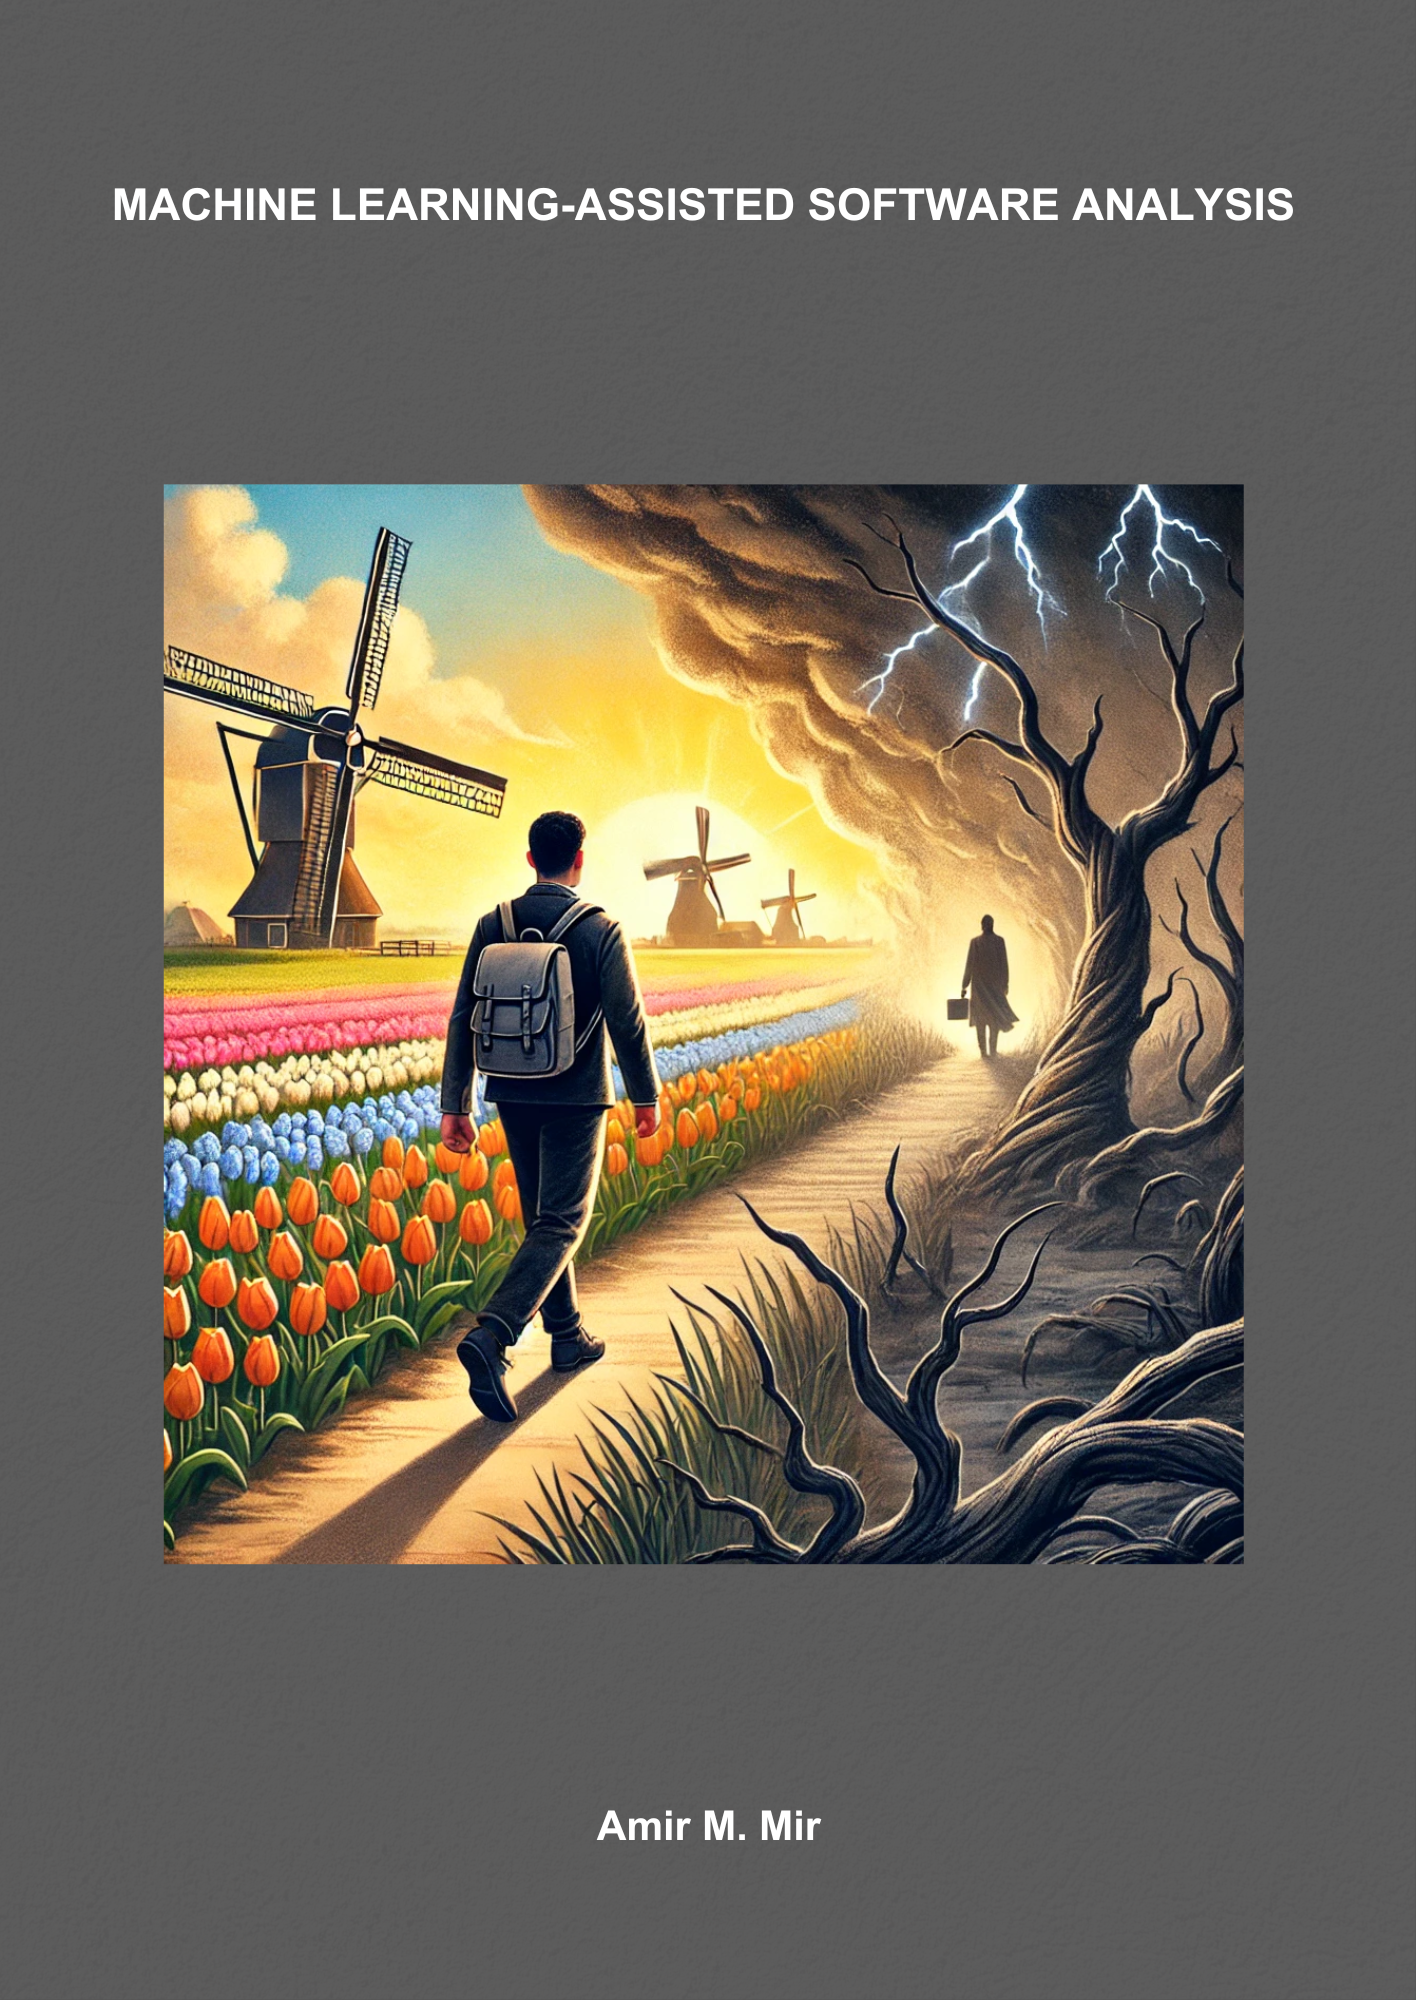
\includepdf{cover/cover-front.pdf}
\begin{titlepage}

\begin{center}

%% Extra whitespace at the top.
\vspace*{2\bigskipamount}

%% Print the title.
{\makeatletter
\titlestyle\bfseries\LARGE\@title
\makeatother}

%% Print the optional subtitle.
{\makeatletter
\ifx\@subtitle\undefined\else
    \bigskip
    \titlefont\titleshape\Large\@subtitle
\fi
\makeatother}

\end{center}

\cleardoublepage
\thispagestyle{empty}

\begin{center}

%% The following lines repeat the previous page exactly.

\vspace*{2\bigskipamount}

%% Print the title.
{\makeatletter
\titlestyle\bfseries\LARGE\@title
\makeatother}

%% Print the optional subtitle.
{\makeatletter
\ifx\@subtitle\undefined\else
    \bigskip
    \titlefont\titleshape\Large\@subtitle
\fi
\makeatother}

%% Uncomment the following lines to insert a vertically centered picture into
%% the title page.
%\vfill
%\includegraphics{title}
\vfill

%% Apart from the names and dates, the following text is dictated by the
%% promotieregelement.

{\Large\titlefont\bfseries Dissertation}

\bigskip
\bigskip

for the purpose of obtaining the degree of doctor

at Delft University of Technology,

by the authority of the Rector Magnificus Prof.dr.ir. T.H.J.J. van der Hagen,

Chair of the Board for Doctorates,

to be defended in a public ceremony

on Thursday, 6 February 2025 at 15:00 o'clock

\bigskip
\bigskip

by

\bigskip
\bigskip

%% Print the full name of the author.
\makeatletter
{\Large\titlefont\bfseries\@firstname\ \titleshape{\MakeUppercase{\@lastname}}}
\makeatother

\bigskip
\bigskip

Master of Science in Computer Engineering - Artificial Intelligence, \\
Azad University (North Tehran Branch), Tehran, Iran \\
Born in Tehran, Iran
%% Extra whitespace at the bottom.
\vspace*{2\bigskipamount}

\end{center}

\clearpage
\thispagestyle{empty}

%% The following line is dictated by the promotieregelement.
\noindent This dissertation has been approved by the promotors.

%% List the promotors (supervisors).
\medskip\noindent
\begin{tabular}{l}
    % Promotor: Prof.\ dr.\ A.\ van Deursen \\
    % Copromotor: Dr.\ ir.\ ing.\ S.\ Proksch \\
    % Copromotor: Dr.\ ir.\ G.\ Gousios
\end{tabular}

\bigskip
% \noindent Independent members:

%% List the committee members, starting with the Rector Magnificus and the
%% promotor(s) and ending with the reserve members.
% \medskip
\noindent
\begin{tabular}{p{4.5cm}l}
    % Rector Magnificus, & Chairperson \\
    % Prof.\ dr.\ A.\ van Deursen, & Technische Universiteit Delft \\
    % Dr.\ ir.\ S.\ Proksch, & Technische Universiteit Delft \\
    % Dr.\ ir.\ G.\ Gousios, & Technische Universiteit Delft \\

    % \medskip
    % External committee members
    % \emph{Onafhankelijke leden:}
    \mbox{\emph{Composition of the doctoral committee:}} & \\
    Rector Magnificus, & Chairperson \\
    Prof.\ dr.\ A.\ van Deursen & Delft University of Technology, promotor \\
    Dr.\ ir.\ S.\ Proksch & Delft University of Technology, copromotor \\
    \mbox{\emph{Independent members:}} & \\
    Prof.\ dr.\ ir.\ F.\ A.\ Kuipers, & Delft University of Technology \\
    Prof.\ dr.\ M.\ Pradel, & University of Stuttgart, Germany \\
    Prof.\ dr.\ P.\ Devanbu, & University of California at Davis, USA \\
    Dr.\ B.\ Ray, & Columbia University, USA \\
    Prof.\ dr.\ A.\ E.\  Zaidman & Delft University of Technology, reserve member \\
    \mbox{\emph{Non-independent members:}} & \\
    Dr.\ ir.\ G.\ Gousios & Delft University of Technology \\
    
    % Prof.\ dr.\ ir.\ E.\ Visser, & Technische Universiteit Delft, reservelid \\ \\

    % \multicolumn{2}{l}{Prof. dr. D. Spinellis has contributed to the end
    % phase of writing \ldots} \\
\end{tabular}

%% Include the following disclaimer for committee members who have contributed
%% to this dissertation. Its formulation is again dictated by the
%% promotieregelement.
%\medskip
%\noindent  %Prof.\ Dr.\ D.\ Spinellis has contributed to the creation of this thesis.

\medskip
\medskip
% TODO Include http://www.win.tue.nl/ipa/?page_id=309
\noindent The work in the thesis has been carried out under the auspices of the research school IPA (Institute for Programming Research and Algorithmics) and was funded by the FASTEN project, a European Union’s Horizon 2020 research and innovation program under grant agreement number 825328.

\medskip
%% Here you can include the logos of any institute that contributed financially
%% to this dissertation.
\vfill
\begin{center}
    
\includegraphics[height=0.5in]{title/logos/tudelft}
    \hspace{2em}
    %\includegraphics[height=0.5in]{title/logos/casimir} \\
    
\includegraphics[height=0.5in]{title/logos/fasten_logo.png}
    \\ \vspace{0.5cm}
    
\includegraphics[height=0.5in]{title/logos/ipa}
    \hspace{2em}
    
\includegraphics[height=0.75in]{title/logos/eu_h2020_logo.png}
\end{center}
\vfill

\noindent
\begin{tabular}{@{}p{0.2\textwidth}@{}p{0.8\textwidth}}
  \textit{Keywords:}  & Machine Learning, Software Analysis, Software Engineering \\[\medskipamount]
      \textit{Printed by:} & ProefschriftMaken (www.proefschriftmaken.nl) \\[\medskipamount]
      \textit{Cover:} & Open AI's DALL·E 3 \\[\medskipamount]
      \textit{Style:} & TU Delft House Style, with modifications by Moritz Beller \\& \url{https://github.com/Inventitech/phd-thesis-template} \\[\medskipamount]
\end{tabular}

\medskip
\medskip
\noindent The author set this thesis in \LaTeX\xspace using the Libertinus and Inconsolata fonts.

\vspace{\bigskipamount}

% Copyrighting this is stupid, questionable, and probably illegal, because large parts of the
% thesis have already been published with the copyright resigning with the publisher.
%\noindent Copyright \textcopyright\ 2015 by A.~Einstein

%% Uncomment the following lines if this dissertation is part of the Casimir PhD
%% Series, or a similar research school.
%\medskip
%\noindent Casimir PhD Series, Delft-Leiden 2015-01

%\medskip
\noindent ISBN 978-94-6518-015-1

\medskip
\noindent An electronic version of this dissertation is available at \\
\url{http://repository.tudelft.nl/}.

\end{titlepage}



%% The (optional) dedication can be used to thank someone or display a
%% significant quotation.
\dedication{\centering \textit{I dedicate my PhD thesis to my mother who unexpectedly passed away at the end of my PhD journey.}}

\tableofcontents

\chapter*{Summary}
\addcontentsline{toc}{chapter}{Summary}
\setheader{Summary}

Software engineering, fundamental to modern technological advancement, profoundly influences various aspects of society by enhancing efficiency, accessibility, and security. This discipline involves systematically applying engineering principles to software systems' design, development, testing, and maintenance. Innovations in software engineering have revolutionized industries such as communication, finance, healthcare, and education, democratizing access to information and connecting global communities. As software systems become increasingly complex, the need for efficient, secure, and reliable software analysis tools becomes paramount.

The thesis focuses on improving the actionability and scalability of software analysis by integrating machine learning (ML) techniques. Traditional static analysis tools often struggle with large codebases, leading to high false positive rates and high computational costs. Machine learning, particularly deep learning architectures like Transformers, offers a promising solution by capturing long-range dependencies in code and learning hierarchical representations. This capability enables ML models to automate tasks such as bug detection, source code summarization, and program repair, providing developers with actionable insights and improving overall productivity and code quality.

A significant contribution of this thesis is the development of ML-based techniques for type inference in Python and call graph pruning. An ML-based type inference approach, namely Type4Py, was proposed, which accurately predicts type annotations for Python code, enhancing code quality and reducing runtime errors. ML models with conservative pruning strategies were proposed for call graph pruning, which learns from dynamic traces obtained by executing programs to identify and eliminate false edges, thereby minimizing false positives and improving precision. Additionally, the thesis explores the application of call graphs in vulnerability analysis, demonstrating that granular assessments provide more accurate and actionable insights than more straightforward, dependency-level analyses.

In summary, this thesis advances the field of software analysis by harnessing machine learning to address two important issues related to the actionability and scalability of software analysis tools. The proposed ML-driven tools and techniques enhance the precision and reliability of software analysis and support developers in maintaining robust, secure, and maintainable software systems. These contributions pave the way for future research in applying ML techniques to various aspects of software engineering, promising further improvements in software development practices.


\chapter*{Samenvatting}
\addcontentsline{toc}{chapter}{Samenvatting}
\setheader{Samenvatting}

{\selectlanguage{dutch}
Software engineering, fundamenteel voor moderne technologische vooruitgang, beïnvloedt diepgaand verschillende aspecten van de samenleving door efficiëntie, toegankelijkheid en veiligheid te verbeteren. Deze discipline omvat het systematisch toepassen van technische principes op het ontwerp, de ontwikkeling, het testen en het onderhoud van softwaresystemen. Innovaties in software engineering hebben industrieën zoals communicatie, financiën, gezondheidszorg en onderwijs gerevolutioneerd, toegang tot informatie gedemocratiseerd en wereldwijde gemeenschappen verbonden. Naarmate softwaresystemen steeds complexer worden, wordt de behoefte aan efficiënte, veilige en betrouwbare software-analysetools steeds belangrijker.

De scriptie richt zich op het verbeteren van de bruikbaarheid en schaalbaarheid van software-analyse door integratie van machine learning (ML) technieken. Traditionele statische analysetools hebben vaak moeite met grote codebases, wat leidt tot hoge foutpositieve percentages en hoge computatiekosten. Machine learning, met name deep learning-architecturen zoals Transformers, biedt een veelbelovende oplossing door langeafstandsafhankelijkheden in code vast te leggen en hiërarchische representaties te leren. Deze mogelijkheid stelt ML-modellen in staat om taken zoals bugdetectie, broncode-samenvatting en programmareparatie te automatiseren, waardoor ontwikkelaars bruikbare inzichten krijgen en de productiviteit en codekwaliteit in het algemeen verbeteren.

Een belangrijke bijdrage van deze scriptie is de ontwikkeling van ML-gebaseerde technieken voor type-inferentie in Python en call graph pruning. Een ML-gebaseerde type-inferentiebenadering, namelijk Type4Py, werd voorgesteld, die nauwkeurig typeannotaties voor Python-code voorspelt, de codekwaliteit verbetert en runtime-fouten vermindert. ML-modellen met conservatieve snoeistrategieën werden voorgesteld voor call graph pruning, die leren van dynamische traceringen verkregen door programma's uit te voeren om valse randen te identificeren en te elimineren, waardoor foutpositieven worden geminimaliseerd en de precisie wordt verbeterd. Daarnaast onderzoekt de scriptie de toepassing van call graphs in kwetsbaarheidsanalyse, waarbij wordt aangetoond dat gedetailleerde beoordelingen nauwkeurigere en bruikbaardere inzichten bieden dan eenvoudigere, afhankelijkheidsniveau-analyses.

Samenvattend, deze scriptie bevordert het veld van software-analyse door machine learning te gebruiken om twee belangrijke problemen met betrekking tot de bruikbaarheid en schaalbaarheid van software-analysetools aan te pakken. De voorgestelde ML-gedreven tools en technieken verbeteren de precisie en betrouwbaarheid van software-analyse en ondersteunen ontwikkelaars bij het onderhouden van robuuste, veilige en onderhoudbare softwaresystemen. Deze bijdragen effenen het pad voor toekomstig onderzoek naar de toepassing van ML-technieken op verschillende aspecten van software engineering, wat verdere verbeteringen in softwareontwikkelingspraktijken belooft.
}




\chapter*{Acknowledgments}
\addcontentsline{toc}{chapter}{Acknowledgments}
\setheader{Acknowledgments}

I am writing an unusually long acknowledgments page in an informal manner, unlike the rest of the thesis. I'll mention the names of many people who have/had been part of my PhD journey and with whom I shared so many memories and nice moments. When writing this page, I'm both happy and sad at the same time. I'm happy because I finished my PhD after 5 years, which is quite an accomplishment for me considering where I come from and the cards I had in my hand to play with. I'm sad because this chapter of my life, my PhD journey, came to an end. If I write a book about my life someday, this will be one of the best chapters to read. I've had a long PhD journey with a mixed bag of successes, failures, tears, laughs, and fears. If I could rewind time, I'd go back to live this chapter 100 times. Anyway, let's talk about my PhD journey and how it began!

In June 2019, I applied for a PhD position at the Software Engineering Research Group (SERG) of TU Delft. \textbf{Georgios Gousios} invited me for an interview. Later, he said Prof. Arie van Deursen would like to talk to you. I spoke to \textbf{Arie}. I never forget this interview in my life. He saw my Master's thesis on GitHub and asked a question about my personal blog. Suddenly, during the interview, a man driving a truck outside our apartment in Tehran was yelling with a big speaker to sell fruits. Arie asked what is this noise and I couldn't really explain it. Thankfully, they both trusted me and offered a PhD position to a young guy from thousands of kilometers away whom they had never met. In the summer of 2019, I did all the paperwork and sold my gaming PC so I could travel to the Netherlands and start my PhD journey there. After getting a temporary visa, on Oct. 10th, 2019 at around 2:20 PM, I arrived in the Netherlands and all I had was small luggage, my master's degree certificate, and a few thousand euros in my pocket.

In my first week, I met \textbf{Pouria Derakhshanfar}, a PhD student at the time, who helped me a lot with onboarding and basic things like even getting lunch since I was coming from a highly sanctioned third-world country, Iran, and I didn't have a debit/credit card to pay. I remember, one day, Pouria was wearing the Last of Us shirt, which made me play this masterpiece game later. Thank you, Pouria, for all the help in the beginning, and you are one of the few people who understand what hardships we have as an international student/immigrant. In late Oct. '19, I met \textbf{Mehdi Keshani} who became my best friend/colleague at TU Delft. I think it's kinda a life miracle that we both ended up working in the same room although Mehdi is just 3 days older than me and he's from a different city, but somehow we never crossed a path in our country but met each other in NL. Mehdi and I shared a lot of moments during our PhD at TU Delft. We laughed, joked, traveled to conferences, had fruitful collaborations, and shared painful times. Thank you, Mehdi, for all the support, understanding, and kindness, especially during the pandemic. In the first two months, I was living with some talented students, \textbf{Mehdi Asadi}, \textbf{Saieed}, \textbf{Hamid}, \textbf{Pouriya Alinaghi}. They helped me a lot in finding a place to live and settle down in Delft.

In the first few months of my PhD, everything was going nicely and I was so excited to start doing a PhD and meeting new people from all around the world. Sadly, in March 2020, a global pandemic happened and we all had to start working from home. During the pandemic, I was one of the very few people who still came to the office to work. At that time, \textbf{Joseph} was my lab/office mate. I was lucky to have him in the office so that I could chat with someone in person during the COVID lockdown. Many thanks to Joseph for all the coffee chats, lunch times, and fun discussions we had during my PhD journey. In 2020, I worked with Georgios, my daily supervisor at the time, and I was part of the Software Analytics lab (SAL). I learned many things from Georgios, including professionalism, pragmatism, efficient communication, and problem-solving. Thanks to Georgios, during the pandemic, I had the chance to hang out with the members of SAL and share good memories with them, namely, \textbf{Ayushi}, \textbf{Elvan}, Mehdi Keshani, \textbf{Maliheh (Mali)}, Joseph, and \textbf{Enrique}.

In March 2021, I started working with \textbf{Sebastian Proksch} who became my main supervisor for the rest of my PhD journey. I spent many hours with Sebastian and we had good chemistry and common interests outside work, which is kinda unusual in a typical supervisor/student relationship. We not only discussed research ideas but also talked about our hobbies like cryptocurrency mining, the latest PC games, and hardware during our coffee chats/breaks. Honestly, I was fortunate to have a supervisor like him who is a PC gamer like myself. Special Thanks to Sebastian for all his direct in-depth feedback and helpful discussions. I hope he'll forget my complaints, laments, and arguments, especially at the end of my PhD journey. Though, I still have one complaint, which is he didn't fulfill my wish, an Nvidia RTX 5090 as a graduation gift. Joking aside, without his massive support and guidance, I would never finish this PhD. 

In 2021, I also met PhD students, \textbf{Ali Khatami}, \textbf{Aru}, \textbf{Mark}, and \textbf{Imara} who joined SERG. I chatted with them many times during our breaks and we shared many good memories at conferences and summer schools. I remember Ali Khatami once approached me to help him with an issue on Linux and I almost erased the whole root filesystem! This is how I also became a Linux admin during my PhD! Ali Khatami is also a cool person to hang out with but, unfortunately, we never went to a concert/festival together, maybe, one day, we'll go somewhere. I know Aru was probably tired of me doing hand hugs with him every time we saw each other at the office. Also, I'm looking forward to having a coffee/drink again with Aru someday in Amsterdam. I know Mark for being very social and keen to learn about other different cultures. I remember walking fast with Imara to the TUD library to grab a "premium" coffee and it was certainly good sport during the working day!

In 2022, I met \textbf{Amir Deljouyi}, \textbf{Shujun}, \textbf{Ali Al-kaswan}, \textbf{Baris}, \textbf{June}, and \textbf{Lorena}. All of them are nice supportive colleagues I had at SERG. Amir is humble and we made jokes and laughed many times at the office. Also, Amir is good at EA FIFA and he annihilated my team several times in this game. One day, I will take revenge! I remember Shujun as one of my office/lab mates and she is very polite and was a Dota 2 player like myself. Ali Al-kaswan was also one of my office mates and friends who tolerated my corny jokes and random chats. Ali and I talked a lot about PC gaming and hardware, and we traveled to very far places in the world like Australia and we shared many nice memories. I definitely miss Ali Al-kaswan as my office mate. I'd like to mention Baris with whom I had good times in Delft. He is a funny cool person, a gamer like myself, had fun at his place several times, and made me laugh many times. If I wanted to invite people to my place, he would be number one on the list. I owe him a nice dinner. June was a very supportive and nice colleague of mine at SERG. She was exactly the postdoc a PhD student needs in hard times to motivate them. She was also great at cracking harsh jokes. Also, I know Lorena for being super polite and her warm personality. I still miss the special Romanian drink she used to share with us.

In 2023, I became colleagues with \textbf{Jonathan}, \textbf{Berkay}, \textbf{Anthony}, \textbf{Aral}, and \textbf{Sara Regali}. Jonathan was also my former Master's student and we became an office mate. He is a humble, dedicated hard-working person and an ML enthusiast. I know Anthony for talking about souls-like games like Elden Ring and how to beat these games. He's also a cool hard-working person, whom I'd like to hang out with. Berkay was one of the few PC gamers at SERG with whom I had coffee chats about games. Yet, I don't know why Berkay is a bit hesitant to say hi to me when we see each other outside the university. Aral was one of the brilliant bachelor students I met at TUD. Aral and I were office mates and we used to play Nintendo games together during our break time. I never had a chance to win a game against Aral. Sara was also visiting SERG to finish her Master's thesis. She was funny and cool. I hope she still remembers what I told her, "Don't forget your former colleague after getting a job in Amsterdam!". I want to mention \textbf{Roham} who is a smart and dedicated bachelor student like Aral. If you, Roham, are reading this, keep up the good work and be consistent. You can achieve 10x what I've done in my life so far when you reach my age, given your solid foundation and the circle of people around you. 

I'd like to mention \textbf{Mitchell}, \textbf{Carol}, \textbf{Leonhard}, the former PhD students at SERG, whom I've known since 2020. I had good memories with all of them, from the summer school in Cordoba, the IPA events, and the SE conferences we attended. During our PhD journeys, we talked about various things and laughed in different places, at coffee machines, bars, restaurants, and zoo. I remember convincing Leonhard that Cyberpunk 2077 was not that buggy at launch! Unfortunately, I haven't talked to him over the past two years but I wish him the best with his new adventure in Singapore. 

After mentioning my peers, I'd like to thank the professors during my time at SERG. First, I thank \textbf{Andy} who, at times, used to challenge me with his critical questions during my presentations. Also, Andy supported my content and posts on social media many times, although he had no obligation to do so. \textbf{Annibale} might be the coolest professor I've ever met in my academic career. I can't count how many times he made us laugh and he was one of the few colleagues I could talk to at the office during the COVID pandemic. Also, his brother, \textbf{Sebastiano} is a great researcher and he was one of the cool people I used to hang out with at the SE conferences/events.  I remember \textbf{Luis} also arrived in NL one month before me and we both knew how it feels to start a new job in another country where you barely know anyone. Although Luis' jokes made me feel a little bit embarrassed at times, he was definitely supportive in hard times. Also, thanks to \textbf{Diomodis} for his great online course on Unix and for inviting me to become a social media co-chair at the MSR'24 conference. I remember \textbf{Thomas} for the coffee chats, grabbing lunch outside, and we also built a PC together at the office. \textbf{Maurício} was always kind and he is also one of the stars in the industry I look up to. Together, we also supervised Jonathan's Master's thesis. I remember \textbf{Burcu} for being super polite, coffee chats, and delicious Turkish delights. Also, many thanks to \textbf{Mali} for inviting me to her research lab's social events. I’ve met very few ambitious hard-working people like Mali. Unfortunately, I didn't have the chance to work with her given that we have similar research interests. Maybe, we'll collaborate in the future.

Also, I'd like to mention the people I know at JetBrains, \textbf{Vladimir}, \textbf{Yaroslav}, and Pouria. They are all very nice and cool people and I hung out with them at the SE conferences. They're so kind to answer my messages quickly on social media despite being super busy. If I had a chance to work at JetBrains, I'd try to join their teams. During my PhD, I worked on the FASTEN project and I had the pleasure of collaborating with SIG, namely, \textbf{Magiel}, \textbf{Chushu}, and \textbf{Miroslav}. They are all professional people, competent industry practitioners, and good at doing business. I also thank \textbf{Paige Bailey} (then-Product Manager of GitHub) for promoting the VSCode extension of Type4Py on X (Twitter), discussing it with her team at Microsoft, and giving us feedback. This helped us to attract Python developers to try the extension before submitting Type4Py's paper to ICSE'22.

I'd like to thank \textbf{Ashwin} whom I first met at the SANER'23 conf. in Macau. We collaborated on ML and software analysis and published two papers. Aside from research, he's also a cool person to hang out with. I'm still looking forward to smoking a cigar with him to celebrate our collaboration. 

Also, I had the pleasure of supervising two wonderful students, \textbf{Evaldas} (bachelor) and \textbf{Lang} (master). I didn't just supervise them but I learned things from them. I'm happy that they're both working on fancy stuff at big tech companies.

A big shout out to the management assistance people at SERG, \textbf{Minaksi} and \textbf{Kim}. They were both kind and handled my inquiries smoothly and efficiently like visa extensions, business travels, paperwork, etc. I still remember Minaksie knocking hard on our door and asking us to join her for a coffee break. Many thanks to both of them.

During my PhD, I was still in touch with my high school friends, \textbf{Morteza} and \textbf{Farzan}. We laughed, yelled, cried, and fought while playing Dota 2. They won't forget the infamous moment I died as Wraith King three times in a row during a match of Dota 2 and I said whatever bad words I knew in Persian! I remember coming back home from work but these two guys never let me feel tired with their jokes and memes. If I go back to Iran one day, I'll visit them to have a high school reunion. Also, shout out to \textbf{Pouya}, a friend of mine, with whom I played Counter Strike 2 and God knows how many players we bothered with our nonsense sayings in the game. People won't forget our ridiculous fights over looting stuff in Arena: Breakout Infinite on your live stream. I remember my "old" friends, \textbf{Ramin} and \textbf{Vahid}, for their emotional support and our daily chats about tech and PC overclocking/benchmarking.

I was also part of the IPA PhD council during my PhD and I would like to thank my peers there, namely, \textbf{Niels}, \textbf{Tom}, \textbf{Ivo}, \textbf{Philip}, \textbf{Christopher}, and \textbf{Lieuwe}. We organized fun social events for the IPA Fall Days. I thank \textbf{Loek}, the then-managing director of the IPA research school for his support and participation in our social games.

I shall mention my aunt, \textbf{Azadeh}, whom I visited many times in Germany during my PhD. It was great to have my aunt close to me and she was like my mother outside Iran. She cooked my favorite Iranian food and was so kind to give me gifts and money, which I didn't need. Also, shout to my cousins \textbf{Sarah} and \textbf{Hossien} with whom I grew up and it was always nice to see them in Germany. It's very sad that my relationship with my aunt was recently sabotaged by some impulsive people in our family.

I can't finish this acknowledgment without thanking \textbf{Arie}, my big boss at TUD. I never forget his massive support during my PhD such as contract extensions and funding my travels. He's a great example of leadership for me. It would've been awesome if I could work with him as a postdoc researcher. 

I'd like to mention the names of my former colleagues at SERG with whom I shared nice moments, from a short coffee chat, to attending local events in NL, and traveling to conferences. I can write sentences about every one of them, but this acknowledgment will become a book in itself. Thanks to \textbf{Fabio}, \textbf{Dimitri}, \textbf{Jean}, \textbf{Vivek}, \textbf{Marielli}, \textbf{Wouter}, \textbf{Xavier}, \textbf{Davide}, \textbf{Xunhui}, \textbf{Gemma}, \textbf{Luca}, \textbf{Anand}, \textbf{Moritz}, \textbf{Quentin}, \textbf{João}, \textbf{Eileen}.

At the end, I'd like to mention the names of the cool PhD students whom I met and hung out with at SE conferences and summer schools. They were doing interesting research. Thanks to \textbf{Sajad}, \textbf{Kevin}, \textbf{Nafiseh}, \textbf{Nathan}, \textbf{Satrio}, \textbf{Cezar}, \textbf{Mahtab (Mattie)}, \textbf{Christian}, \textbf{Pooya Rostami}, \textbf{Gunnar}.

To wrap this up, I thank the independent members of my PhD committee, \textbf{Fernando Kuipers}, \textbf{
Michael Pradel}, \textbf{Prem Devanbu}, and \textbf{Baishakhi Ray} for examining my PhD thesis and their invaluable feedback.

Wait a second! I thanked many people here but myself! I worked hard to reach this point in my life where I have the luxury of obtaining a PhD degree. But this is not the end of the movie (I hope!). The next chapter has already begun for me. However, the picture I have for my future in my mind is not crystal clear. In life, you never truly know where your boat might crash or arrive in one piece in a stormy ocean. Life is generally way more complex than the research problems I addressed in this thesis. Although one may do every step perfectly, life can still surprise them in a way that they didn't expect. I'm not a perfect human and had "mistakes" that I could probably avoid (you're never gonna find a mistake in this thesis!). I should probably "punish" myself for the things I did wrong, instead of blaming others or expecting people to do me a favor! As the cliché goes, your biggest "enemy" is the person in the mirror. There are many aspects in doing a PhD and one of them is doing novel research. Some say doing a PhD is a lonely journey but it's not! I can't deny that the people around you will have an influence on you (in)directly and little or big. I don't wanna lecture you here about what you should do right in a PhD journey. It's just beyond the scope of this thesis. In the near future, I should write a blog post about my mistakes and failures during this journey. On the other hand, If the concept of destiny exists, there were probably no mistakes in things I did in my life. Maybe, I was supposed to do whatever I did and there are no alternative life paths for me. If I could go back in time, I'd probably end up writing this sentence again. This is also a reason why I'm not really jealous of anyone. They may live their own life path and I do mine. I'm genuinely happy that I met all of these people mentioned in this section. There are billions of other people on the Earth whom I'm never gonna meet. Somehow, my life path crossed theirs. All of them have their own story and certainly, they have something to teach me. Regardless of destiny, I hope you won't see me soon saying "How the heck I ended up here! This ain't supposed to be my future!". Anyhow, these are some of my thoughts on life, and thanks for reading my ramblings/rants. Of course, you can ignore whatever I said. Perhaps, the most important lesson I learned by doing a PhD was to think critically for myself before accepting blindly whatever I read or hear.

\begin{flushright}
{\makeatletter\itshape
    Amir \\
    Delft,  January 2025
\makeatother}
\end{flushright}




%% Use Arabic numerals for the page numbers of the chapters.
\mainmatter

%% Turn on thumb indices.
\thumbtrue

\NewDocumentCommand\RQ{+m}{{\bf RQ$_{#1}$}}

\chapter{Introduction}
\label{ch:intro}

% \begin{abstract}
% Sample Abstract.
% \end{abstract}

Software engineering, a cornerstone of modern technological advancement, plays a pivotal role in shaping society. It involves the systematic application of engineering principles to the design, development, testing, and maintenance of software~\cite{ianbook}. This discipline not only focuses on functionality and performance but also on ensuring the reliability and security of software systems. As a result, software engineers have created complex systems that power everything from global communication networks and financial systems to personal computing devices and medical equipment~\cite{ke2012software, rausch2013software}.

The impact of software engineering on society is profound and multifaceted. It has drastically transformed how we work, communicate, and live, making processes more efficient and information more accessible~\cite{ianbook}. Innovations such as the internet, mobile applications, and cloud computing, all software engineering products, have revolutionized industries such as
computer games, music, and film and television~\cite{vaudour2020software}. Moreover, these advances have democratized access to information, connected global communities, and facilitated advancements in other fields such as healthcare, education, and transportation~\cite{xu2018industry}.

Building on the foundational aspects of software engineering, software analysis is a critical component that ensures software systems are efficient, secure, and error-free. This analytical process includes analyses such as type inference and call graph construction, which help optimize code and enhance its performance~\cite{nielson2015principles}. Type inference automatically determines the types of expressions in a programming language without explicit type annotations, simplifying code maintenance and improving readability. Call graph construction, meanwhile, focuses on finding all possible function calls within a program, providing a visual and analytical map that developers use to optimize execution paths and enhance performance~\cite{ryder1979constructing}.

The actionability of software analysis tools is a critical factor influencing their adoption and effectiveness in software development. Actionability refers to the tool's ability to provide developers with clear, practical steps to resolve detected issues. This is vital because actionable warnings help developers quickly understand and address problems, thus enhancing productivity and code quality. Conversely, false warnings, or false positives, are instances where the tool incorrectly flags non-issues as problems. High rates of false positives can lead to "alert fatigue," where developers become desensitized to warnings and may start ignoring or turning off the analysis tools altogether. Minimizing false warnings and maximizing actionability are prominent. Tools that produce too many false positives are seen as unreliable and can erode trust among developers, leading to decreased usage and effectiveness. On the other hand, tools with high actionability support developers in maintaining and improving code quality. Balancing these factors is crucial for the practical adoption of static analysis tools in real-world software development environments~\cite{christakis2016developers, johnson2013don}.

Scalability is a significant problem in software analysis due to large-scale software systems' increasing complexity and resource demands. Larger codebases mean more lines of code, more functions, and more intricate interdependencies to analyze, all requiring considerable processing power and time. Also, maintaining up-to-date analysis in the face of frequent incremental changes, such as new features and bug fixes, poses another scalability challenge. Ensuring accurate analysis without reprocessing the entire codebase necessitates sophisticated techniques for partial analysis and data caching. Balancing precision and performance becomes increasingly difficult as more detailed analyses demand significant computation. 

Recently, machine learning has shown impressive performance in tackling various tasks in software analysis, particularly those involving the examination and manipulation of source code. Over recent years, the use of ML techniques for software analysis tasks has expanded and diversified significantly. These tasks include but are not limited to automated testing, bug detection, source code summarization, program repair, and type inference~\cite{sharma2024}. The success of ML in software analysis largely derives from its ability to learn from vast datasets of source code, which subsequently facilitates the automation of traditionally manual and error-prone tasks. For instance, ML methods have been applied to enhance software testing by automating the generation of test cases and optimizing testing workflows~\cite{schafer2023empirical}. Additionally, in the area of program repair, ML models are trained to predict and rectify bugs automatically, significantly reducing the manual effort required in debugging.

A key advantage of ML in this domain is its ability to provide actionable predictions that directly aid developers. For instance, in bug detection, ML models can be trained on large codebases to learn patterns associated with common bugs. When analyzing a new program, these models do not just flag potential issues but can pinpoint specific lines or methods likely containing bugs or vulnerabilities~\cite {fu2022linevul}, offering developers concrete starting points for debugging. Similarly, in program repair tasks, ML models trained on pairs of buggy and corrected code can suggest exact changes, such as modifying a condition in an if-statement or adding a null check—providing developers with ready-to-implement fixes~\cite{zhang2023survey}.

Moreover, ML models scale better with the size and complexity of programs. As mentioned, traditional static analysis tools often struggle with large codebases, as their rule-based approaches lead to exponential growth in analysis time or a surge in false positives. In contrast, ML models, particularly those based on deep learning architectures like transformers, excel at capturing long-range dependencies in code~\cite{maunveiling}. When trained on diverse, large-scale datasets, these models learn hierarchical representations, from token-level patterns to class-level structures, enabling them to understand the context of a given code snippet within its broader class or module. This hierarchical learning allows ML models to maintain high accuracy even when analyzing large programs. 

In this thesis, we aim to improve the actionability and scalability of software analysis by leveraging the power of machine learning. Our primary focus is on addressing two significant challenges: improving type inference for Python and refining call graph construction. These areas present substantial uncertainty, particularly in the realms of predicting type annotations accurately and constructing call graphs precisely. Python's dynamic nature and flexibility can lead to ambiguous type information, making traditional static analysis methods less effective. This ambiguity can cause issues such as missed type errors and less efficient code analysis, ultimately impacting code quality. To mitigate these uncertainties, we seek to explore ML-based techniques to predict type annotations in Python code. Machine learning models can learn from vast amounts of code corpus to identify patterns and infer types more accurately than traditional heuristic-based methods. By doing so, we aim to improve code quality, reduce runtime errors, and enhance the developer experience through more accurate code analysis and features like auto-completion.

Similarly, call graph construction faces challenges due to dynamic method calls and runtime behavior that static analysis may over-approximate. Traditional static analysis can result in call graphs with unnecessary or false edges, leading to false positives and reduced trust in the analysis tools. We propose employing machine learning models to analyze dynamic traces from program executions. By integrating insights from these dynamic traces, we can refine static call graphs, pruning unnecessary or false edges, and thereby reducing false positives. Our approach aims to align with developer preferences for fewer false alerts, increasing the trust and reliance on software analysis tools. We anticipate that enhancing the precision of call graphs will positively impact various downstream analyses, such as security assessments, making them more efficient and actionable. Machine learning offers a promising solution to handle the inherent uncertainties in software analysis, providing a more robust and scalable approach to improving type inference and call graph construction.

Additionally, we explore the application of call graphs in vulnerability analysis. Our approach involves adopting a granular methodology to identify at-risk Maven packages accurately, demonstrating that the value of granular vulnerability assessments over simpler, dependency-level analyses. Through this work, we aim to highlight the value of fine-grained vulnerability assessments in offering actionable insights for improving security practices in software development. Overall, this thesis aspires to push the boundaries of software analysis by developing powerful, ML-driven tools. These tools are intended to empower developers to build robust, secure, and maintainable software systems, addressing the pressing challenges of modern software development with promising solutions.

\section{Background}
Software analysis is a critical phase in the software development lifecycle that involves examining and evaluating a software product to understand its structure, functionality, and behavior. This process is essential for identifying potential issues, ensuring compliance with specifications, and verifying that the software meets its intended objectives. Software analysis can be divided into various forms, including static, dynamic, and formal methods, each serving unique purposes and providing different insights into the software system.

Static analysis refers to examining the software's behavior without executing the program. This type of analysis is conducted using tools that inspect the source code to detect possible vulnerabilities, coding errors, and style issues. It is beneficial for finding syntax errors, type mismatches, and other anomalies that could lead to software failure, all of which can be identified without running the program. Static analysis tools automate much of the review process, enabling developers to identify issues early in the development cycle. This not only helps in improving code quality but also reduces the time and cost associated with later stages of testing and maintenance.

On the other hand, dynamic analysis involves analyzing the software while it is running. This method checks the software's behavior in a real-time environment and validates its output against expected results. Dynamic analysis is crucial for identifying issues that may not be evident through static analysis alone, such as memory leaks, performance bottlenecks, and concurrency issues~\cite{orton2022dynamic}. Tools used for dynamic analysis can simulate a range of conditions under which the software might operate. They can help verify the software's functional correctness, ensuring it behaves as expected under different scenarios.

Together, these two methods form a comprehensive approach to software evaluation, each contributing uniquely to the overall quality and reliability of the final product. By integrating static and dynamic analysis, developers can better understand the software’s operational characteristics and potential weaknesses, leading to more robust and error-free software.

\subsection{Call Graph Construction}
A call graph is a crucial compile-time abstraction in software analysis, representing the calling relationships among the procedures or methods in a program. It comprises nodes (procedures or methods) and directed edges (calls from one procedure to another). Constructing call graphs involves analyzing the program’s source code to determine these relationships. While this is straightforward in procedural languages where calls are explicit, this task becomes complex in object-oriented languages due to dynamic dispatch or first-class functions~\cite{grove1997call}.

Control Flow Analysis (CFA) is integral to constructing call graphs in these complex scenarios. CFA assesses the flow of calls and the potential value expressions that might be taken at various program points. In languages that support dynamic features, determining the targets of calls involves sophisticated inference of possible function or method targets dynamically determined by runtime data. The level of CFA can vary from simple, context-insensitive analyses (0-CFA) to more detailed but computationally intensive context-sensitive analyses (k-CFA)~\cite{shivers1991control}.

The construction of call graphs often involves a trade-off between precision and soundness. Call graphs are over-approximated to include potential calls that may never actually occur in any execution of the program, ensuring that all actual calls are represented but possibly including false positives, harming precision. A sound call graph guarantees that it accurately reflects all potential executions of the program, which is particularly critical in security-focused applications~\cite{sui2020recall}.

The applications of call graphs extend across several domains. Compilers use them to optimize code by enabling function inlining, dead code elimination, and recursion optimization. They are also used in software maintenance to aid in understanding and modifying code, in security to identify potential vulnerabilities, and in generating automated documentation to aid in program understanding. However, the construction and use of call graphs in dynamic or complex environments pose ongoing challenges. Balancing the precision of call graphs without significantly impacting performance and adapting call graph analyses to modern programming paradigms like asynchronous programming and microservices are areas of active research~\cite{luo2022depth}. New algorithms that effectively balance precision, scalability, and computational overhead are continually explored to improve call graph generation.

% \begin{tcolorbox}
% \textbf{Research Problem}: Over-approximation in call graphs involves including more potential calls than might actually occur during the execution of a program. This hampers precision in call graphs and leads to false positives or warnings in client analyses. 
% \end{tcolorbox}

\subsection{Type Inference}
Type inference is used in programming languages to determine the types of expressions without explicit type annotations automatically. This technique is fundamental in statically typed languages, where every variable and expression type must be known at compile-time. It is also increasingly applied in dynamically typed languages, such as Python's PEP 484~\cite{van2014pep}, TypeScript~\cite{bierman2014understanding}, and PHP~\cite{phptd}, to improve performance and provide early error detection. Type inference enhances language usability by reducing code verbosity and facilitating generic programming, allowing developers to write more abstract and flexible code without the overhead of constant type declarations.

The challenges of type inference stem from the complexity and diversity of programming language features. One primary challenge is balancing type inference precision with complexity. More sophisticated type systems, which include features like generics, union types, or intersection types, require more complex inference algorithms, impacting the compiler's performance and the clarity of error messages. Additionally, features such as polymorphism, higher-order functions, and implicit conversions can complicate the inference process, necessitating advanced algorithms like constraint-based type inference or type hints to guide the process effectively~\cite{agesen1995cartesian}.

In dynamically typed languages, the challenges of type inference are amplified by their flexible type systems. For example, Python supports features such as duck typing, where an object's operations are determined by its current attributes rather than its type. This flexibility complicates type inference, as a variable's type can change over its lifetime, and mixed-type containers can further obscure type flows. Python also allows runtime behaviors like dynamically adding attributes to objects and supports first-class functions~\cite{peng2021empirical}, which can be created and passed around at runtime like other objects. Similarly, TypeScript and PHP introduce complexities with their dynamic typing and runtime behaviors. These characteristics make static type inference particularly challenging because type information can change during execution.

\subsection{Machine learning for software analysis}
Machine learning has advanced the state-of-the-art in various domains~\cite{dargan2020survey}, namely, image, text, and speech, including software engineering, where it significantly enhances source code analysis. Integrating ML techniques into software analysis tasks utilizes the ability of these models to recognize patterns and make predictions based on big code corpus. This intersection of ML and software engineering, known as Machine Learning for Software Engineering (ML4SE), has recently experienced considerable growth due to advancements in ML algorithms, the increased availability of open-source code, and improvements in compute resources~\cite{sharma2024}.

One primary motivation for incorporating ML into software analysis is the complexity and size of modern software systems, which render traditional analysis methods less effective and scalable. ML techniques can automate various tasks such as bug detection, code completion, refactoring, and vulnerability analysis by learning from historical code data and identifying patterns that indicate potential issues. For instance, deep learning models, a specialized subset of ML, have demonstrated significant potential in understanding and generating code, thereby assisting in tasks like code summarization and synthesis~\cite{le2020deep}.

A crucial concept within ML4SE is software naturalness. Traditional software analysis relies on rigorous, logical approaches, such as gathering and resolving constraints related to a program. This method is particularly effective for proving that certain parts of the code are unreachable and can thus be eliminated. However, only some problems fit into this structured approach. Issues involving human factors or lacking a definitive correct solution are often more amenable to statistical techniques~\cite{pradel2021neural}. For instance, determining the most "natural" name for a specific variable is a task better suited for these methods. Recently, deep neural networks have become a potent tool in this realm, leading to the development of neural software analysis. In this context, machine learning models are trained using vast quantities of program data annotated with the desired analysis results. These models are then applied to new, unseen problems, effectively leveraging the concept of software naturalness to improve code readability, maintainability, and overall quality. This approach complements traditional methods and addresses their limitations by providing more flexible and adaptive solutions for complex, real-world software engineering challenges.

The advantages of ML for source code analysis are evident in the improvements in efficiency and accuracy reported in numerous studies. By automating routine tasks, ML allows developers to concentrate on more creative aspects of software development. Furthermore, the predictive capabilities of ML models facilitate the early detection of defects and vulnerabilities, thereby enhancing software quality and security. To this end, researchers have employed various ML techniques, ranging from traditional models like Decision Trees and Support Vector Machines to advanced neural networks such as Convolutional Neural Networks (CNNs) and Recurrent Neural Networks (RNNs), Large Language Models (LLMs), each tailored to specific analysis tasks. Despite these advancements, the field faces several challenges, including the necessity for large, labeled datasets, the interpretability of ML models, and integrating these models into existing development workflows~\cite{gao2023interpretability}.

\subsection{Software Ecosystem}
Software ecosystems encompass an interconnected network of software components, libraries, and tools that developers use to build and maintain applications~\cite{mensbook}. A common approach to software reuse within these ecosystems involves incorporating open-source software (OSS) libraries from centralized code repositories like Maven or PyPI. Developers simply list the third-party libraries on which their project depends, and automated tools fetch these libraries into the project’s development environment. However, significant incidents like the LeftPad event~\cite{leftpad}, which caused numerous websites to malfunction, the Equifax security breach, which compromised vast numbers of credit card details, the Log4j incident in 2021~\cite{log4j}, which exposed millions of systems to potential cyberattacks, and the newly discovered vulnerability in XZ utils identified in 2024~\cite{xz}, have shown that relying on external software libraries can pose considerable operational and compliance risks. These incidents also highlight the challenges in assessing the security risks associated with these dependencies.

Addressing these challenges is crucial for software development firms to deliver high-quality products rapidly. By tackling the issues associated with OSS dependencies, companies can confidently leverage the benefits of open-source code, such as reduced development costs and faster time-to-market, without compromising on security and compliance. In response to these pressing needs, the FASTEN project~\cite{fasten}, Fine-Grained Analysis of Software Ecosystems as Networks, has developed a comprehensive solution by providing fine-grained, method-level tracking of dependencies, going beyond the capabilities of existing dependency management systems. By offering a more granular and robust approach to managing OSS dependencies securely, FASTEN empowers software development firms to mitigate the risks associated with external libraries while reaping open-source software's benefits. This solution has the potential to revolutionize the way companies handle OSS dependencies, ensuring a more secure and efficient software development process.

The FASTEN project funds this thesis, a European
Union’s Horizon 2020 (Grant No. 825328). The core idea of FASTEN is to make dependency management more robust and intelligent by tracking program dependencies at the call graph level. Specifically, the project performs more sophisticated analyses of i) security vulnerability propagation, ii) licensing compliance, and iii) dependency risk profiles. To accommodate adoption, FASTEN integrates those analyses into popular package managers, namely, Maven, PyPi, and Debian, to help developers manage their program's dependencies more confidently. More specifically, The FASTEN approach goes beyond the capabilities of existing dependency management systems by:

\begin{itemize}
    \item Creating sound call graphs that show exactly which methods in external libraries or dependencies are being used by the project.
    \item Enabling more accurate vulnerability propagation analysis by tracing the call paths to which vulnerabilities could affect the methods.
    \item Allowing for more nuanced dependency risk profiles based on the actual usage patterns of code from third-party libraries.
    \item Facilitating more precise licensing compliance checks by identifying which library files are in use.
\end{itemize}

% \begin{tcolorbox}
% \textbf{Research Problem}: Python's support for features like duck typing and dynamic attribute addition introduces significant complexity to static type inference, as types can potentially change throughout a variable's lifetime, and operations are determined more by present attributes than by fixed types. Furthermore, Python’s use of mixed-type containers and first-class functions, which can be dynamically created and manipulated, adds layers of uncertainty to the process of accurately inferring types.
% \end{tcolorbox}

\section{Research Direction}
% \subsection{Research Hypotheses}
% Given the enormous success of machine learning in natural language tasks~\cite{otter2020survey, min2023recent}, we form two research hypotheses that machine learning is promising in solving software analysis tasks like inferring type annotations for Python and pruning edges in static call graphs. As mentioned, software is also natural, meaning it has predictable and regular patterns that machine learning models can learn.

% \subsection{Research Questions}
% The main objectives of this thesis are:

% \begin{enumerate}
%     \item Use machine learning techniques to overcome challenges of type inference for dynamic languages such as Python.
%     \item Investigate the effectiveness of machine learning techniques for pruning call graph edges and propose a conservative solution to minimize the loss in soundness after pruning.
%     \item Propose a non-learning-based CG pruning technique based on class hierarchy and compare it with the ML-based techniques.
%     \item Investigate the applicability of learning-based CG pruning techniques to security applications such as vulnerability propagation.
%     \item Compare the dependency- and call graph-level vulnerability assessment in the Maven ecosystem.
% \end{enumerate}

In this thesis, we explore two main research directions, type inference for Python and call graph pruning as follows:

\paragraph{Machine learning-based type inference for Python}
Machine learning can help infer type annotations for Python by learning from large codebases that contain explicit type annotations or inferred types. ML models trained on these annotations can predict the types of variables, function return values, and arguments in code. This helps reduce runtime errors by enabling early detection of type mismatches. It enhances programming environments through features like auto-completion and more accurate code analysis, making the development process more efficient and less error-prone.

\paragraph{Machine learning-based call graph pruning}
Machine learning offers a promising solution for pruning call graphs by analyzing dynamic traces from program executions to identify unnecessary or false edges in statically constructed call graphs. By doing so, ML can help reduce the over-approximation typically seen in static call graph constructions, thereby minimizing the number of false positives. This reduction is critical as it aligns with developer preferences for fewer false alerts~\cite{christakis2016developers}, which can enhance trust and reliance on software analysis tools. Enhanced precision in call graphs would also benefit downstream analyses like security analysis, making it faster and more actionable.

In this thesis, we also aim to answer the following high-level research questions:

\begin{description}
    \item[\RQ{1}] How effective is call graph pruning for security-focused applications?
\end{description}

\noindent
The motivation for exploring the effectiveness of call graph pruning in security-focused applications arises from the need to enhance the efficiency and scalability of security analyses in software systems. Call graphs are fundamental in various security-related analyses, such as vulnerability detection and malware analysis. However, these graphs can become exceedingly big and complex, especially in large software systems, leading to significant computational overhead and slower analysis time. By employing call graph pruning techniques, which strategically remove irrelevant or less critical nodes and edges from the graph, it is hypothesized that the resulting simplified graph will retain essential information for security tasks while being significantly smaller. This reduction could also speed up security analyses considerably.

\begin{description}
     \item[\RQ{2}] How does the call graph-based approach aid in reducing false positives in the vulnerability propagation analysis?
\end{description}

\noindent
While helpful in identifying potential security risks, traditional dependency analyses often lack the precision and context needed to accurately trace how vulnerabilities might propagate through actual execution paths in software. This inherent limitation in naive dependency-level analyses has motivated us to study how call graph-based approaches can reduce false positives in vulnerability propagation analysis. Call graphs provide a more nuanced and accurate representation by mapping the potential interactions between functions within an application as they occur during execution. This fine-grained approach allows for a more targeted analysis, potentially distinguishing between genuine vulnerabilities and benign code behaviors. By leveraging call graphs, security analysts can more effectively pinpoint the paths that a vulnerability may actually traverse, thereby reducing the incidence of false positives, which are common in broader, dependency-based approaches. The fine-grained approach enhances the effectiveness of security measures and optimizes the allocation of resources toward addressing the most critical vulnerabilities first.
    
\begin{description}
    \item[\RQ{3}] How effective is machine learning in inferring type annotations for Python?
\end{description}

\noindent
 While flexible, Python's dynamic typing system can lead to ambiguities that need to be clarified for the intent and correctness of code, particularly in large and complex codebases. As mentioned previously, type annotations in Python help programmers to explicitly declare the intended data type of variables and function parameters, thus enhancing code clarity, reducing errors, and facilitating better tooling for static analysis such as code completion. However, manually annotating types can be laborious and prone to human errors. We hypothesize that machine learning presents a promising solution to this challenge by potentially automating the inference of type annotations. By analyzing a large Python code corpus, machine learning models could learn patterns and contexts that dictate variable types, aiding in automatically generating type annotations with high accuracy. This can ultimately boost developers' productivity, improve code quality, and bolster the overall robustness of Python applications.

% TODO: vulnerability propagation analysis 
\section{Research Methodology}
This thesis adapts the common research methodology used in (machine learning for) software engineering papers, which often involves three main steps: mining software repositories, training ML models, and performance evaluation. We explain each of these steps as follows.

\paragraph{Mining software repositories} Mining software repositories involves extracting and analyzing data from version control systems like GitHub to understand software development practices and trends. This process includes collecting information such as code commits, issues, pull requests, and other metadata. By analyzing this data, researchers and developers can identify patterns, detect bugs, measure productivity, and gain insights into software evolution~\cite{kalliamvakou2016depth}. Tools and techniques used for mining can range from simple scripts to advanced machine learning algorithms, which help in automating the extraction and analysis of large volumes of data efficiently.

For this thesis, we will specifically create datasets for training ML models by either analyzing Abstract Syntax Trees (ASTs) or dynamic call graphs, which involves parsing the source code into its syntactic structure or execution flow. ASTs represent the hierarchical structure of the code, capturing the syntactic relationships between different code elements, which can be used to understand code semantics and identify potential patterns for machine learning models. On the other hand, dynamic call graphs represent the runtime interactions between different parts of the code, providing insights into the actual execution paths and dependencies. These representations can be transformed into feature sets suitable for machine learning, enabling the training of models for tasks such as type inference and call graph pruning.

\paragraph{Training machine learning models} Training deep learning techniques for software analysis tasks involves leveraging (large-scale) datasets of source code to teach models to understand and generate code. Deep learning models, particularly those based on architectures like Transformers~\cite{vaswani2017attention}, can be pre-trained on extensive corpora of code from repositories such as GitHub. These models learn code's syntactic and semantic patterns, enabling them to perform various tasks~\cite{maunveiling}. Fine-tuning these pre-trained models on specific tasks, such as type inference or call graph pruning, requires additional task-specific data. For type inference, the model learns to predict the data types of variables in dynamically typed languages, improving code comprehension. Fine-tuning for this task involves providing examples of code with explicit type annotations.

Dynamic call graphs represent the execution behavior of a program at runtime by capturing the interactions between different functions or methods during execution (i.e., running unit tests). Fine-tuning code language models to prune edges in these call graphs involves training the models to identify and remove irrelevant calls. This pruning enhances the precision of downstream analysis and reduces computational overhead. The process involves feeding the model examples of dynamic call graphs with annotated edges indicating which calls are essential and which are false. By learning these patterns, the model can accurately predict and prune unnecessary edges in unseen call graphs, thus improving the overall usability of program analysis tools. This approach leverages transfer learning, where a pre-trained model is adapted to new, related tasks, resulting in fine-tuned models that aid significantly in the aforementioned code-related tasks.

\paragraph{Performance evaluation} We will assess trained ML models for tasks like type inference and call graph pruning from two key perspectives: \textit{accuracy} and \textit{scalability}. Accuracy refers to the model's ability to perform the task for which it was trained correctly. For type inference, accuracy is measured by how effectively the model predicts the data types of variables in dynamically typed languages, often benchmarked against a labeled dataset with known type annotations. High accuracy in type inference translates to fewer errors in predicted types, leading to more robust and maintainable code. For call graph pruning, accuracy is evaluated based on the model’s ability to correctly identify and remove irrelevant or false calls, ensuring that the essential execution paths are preserved while unnecessary calls are removed. Precision, recall, and F1 score are standard metrics that quantify accuracy in these contexts.

Scalability, on the other hand, examines how fast the model performs as the size of the input data increases. A scalable model for type inference should reasonably be fast even when analyzing large codebases with thousands of lines of code. Similarly, for call graph pruning, scalability is assessed by the model's ability to handle large static call graphs. This includes the model's computational requirements and how effectively it can process and prune large call graphs within a reasonable time frame. Evaluating both accuracy and scalability ensures that the ML-based software analysis techniques are accurate in their predictions and practical for real-world applications involving large-scale software systems.

\section{Thesis Overview}
Figure~\ref{intro:fig:overall} shows an overview of the work presented in this thesis, which is divided into two parts, proposed techniques and explored applications. The thesis is organized as follows.

\begin{figure}[!t]
 \centering
 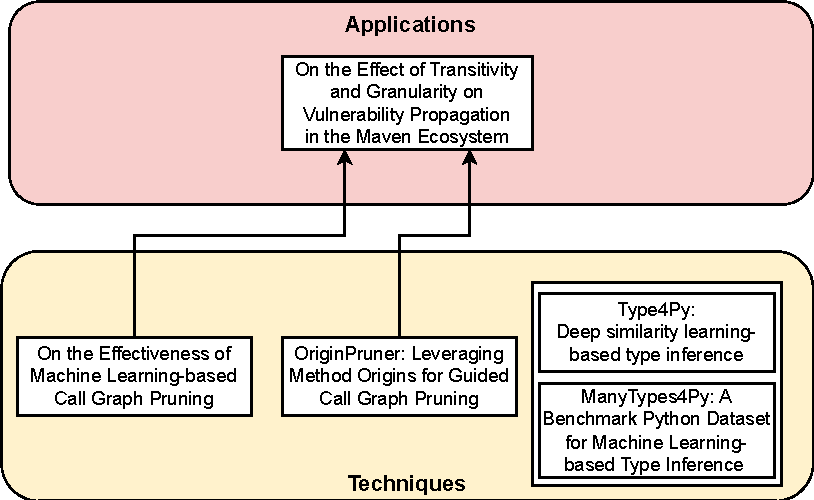
\includegraphics[width=\linewidth]{introduction/figs/thesis_overview.pdf}
 \caption{Overview of this PhD thesis.}
 \label{intro:fig:overall}
\end{figure}

\begin{itemize}
     \item In Chapter~\ref{ch:effect_ml_cg_pruning}, we addressed the RQ1 and conducted an empirical study on the effectiveness of ML-based call graph pruning. We addressed the limitations of previous research, such as a lack of a benchmark dataset, imbalanced training data, and reduced recall, which impacts practical downstream applications. To overcome these challenges, the study introduces the NYXCorpus, a new dataset comprising real-world Java programs with comprehensive test coverage. Our work also explores conservative pruning strategies during both the training and inference phases of ML-based CG pruners to improve the balance between recall and precision. Findings reveal the inherent difficulties of CG pruning in real-world Java projects, showing substantial improvements in precision at the cost of reduced recall. Despite these challenges, pruned CGs demonstrate comparable quality to those produced by context-sensitive 1-CFA analysis but are significantly smaller and faster to generate, offering nearly identical outcomes in downstream analyses. Using the proposed conservative strategies, ML-based CG pruning can achieve a more efficient balance between precision and recall, thereby enhancing the utility of static CGs in practical downstream applications.
    
    \item In Chapter~\ref{ch:origin_pruner}, we also addressed RQ1 and presented \tool{OriginPruner}, a novel technique for pruning edges in static call graphs. Static CGs commonly face challenges like over-approximation, which compromises their utility by inflating their size and introducing imprecision. \tool{OriginPruner} leverages the concept of method origin, identifying methods that introduce a signature within a class hierarchy and are often overridden to prune false edges effectively. Additionally, by integrating localness analysis, which assesses the scope of method interactions, \tool{OriginPruner} can confidently identify and eliminate edges related to origin methods, thereby enhancing CG precision. Key findings show that specific dominant origin methods, such as \texttt{Iterator.next}, significantly influence CG sizes; the derivatives of such origin methods are predominantly local, allowing for their safe pruning without detrimentally impacting downstream inter-procedural analyses. Also, \tool{OriginPruner} can significantly reduce CG size while preserving the soundness required for security applications like vulnerability propagation analysis, and it achieves these improvements with minimal computational overhead. These findings imply that incorporating domain knowledge about the type system into CG pruning strategies offers a viable and promising path for enhancing the performance of static program analysis.
    
    \item In Chapter~\ref{ch:effect_trans_gran}, we addressed RQ2 and explored the application of call graphs in vulnerability analysis and studied the effect of transitivity and granularity on vulnerability propagation in the Maven ecosystem. Past studies assess vulnerability impact at the dependency level, which arguably overestimates the actual risk to projects. Focusing on the Maven ecosystem, we adopt a more granular approach by analyzing a dataset of 3 million recent Maven packages, including their full transitive dependencies, to construct call graphs and perform reachability analysis. This allows for a more accurate identification of genuinely at-risk Maven packages. The findings reveal that while a significant portion of packages appears vulnerable when considering all transitive dependencies, a small percentage have reachable paths to vulnerable code, indicating a lower risk than previously found. Also, limiting dependency tree depth could efficiently reduce the computational load of a granular analysis. The chapter concludes with implications for software engineering, highlighting the value of granular vulnerability assessments over simpler, dependency-level analyses, providing actionable insights for improving security practices in software development. 

    \item In Chapter~\ref{ch:t4py}, we addressed RQ3 and proposed \tool{Type4Py}, a deep similarity learning-based hierarchical neural network model. While enhancing developer flexibility and productivity, the lack of static typing in dynamic languages like Python can lead to runtime exceptions. Python's PEP 484 introduced optional type annotations as a means to address these issues. However, it is a daunting task to retrofit types into existing codebases manually. \tool{Type4Py} learns to distinguish between similar and dissimilar types in high-dimensional space, facilitating type inference through the nearest-neighbor search. Unlike the previous work, which relied on potentially unsound human-provided type annotations, \tool{Type4Py} is trained and evaluated on a type-checked dataset, offering a more reliable assessment of its practicality through mean reciprocal rank (MRR). Empirical results show that \tool{Type4Py} significantly outperforms state-of-the-art approaches, achieving a substantial increase in MRR, therefore indicating its effectiveness in inferring type annotations. Additionally, the chapter discusses the development of a Visual Studio Code extension that employs \tool{Type4Py} to assist developers with ML-based type auto-completion for Python, further aiding in retrofitting types into existing codebases and enhancing productivity and code quality. \tool{Type4Py}'s inferred types can be used to aid applications like call graph construction and unit test generation for Python. In this thesis, we have not explored these applications. 
\end{itemize}

Also, Table~\ref{tab:chap-methods} shows research methods used in each chapter.

\begin{table}[ht]
\centering
\resizebox{\textwidth}{!}{\begin{tabular}{@{}lccc@{}}
\toprule
\textbf{Chapter} & \textbf{Mining Software Repositories} & \textbf{Training ML Models} & \textbf{Performance Evaluation} \\ \midrule
Chapter~\ref{ch:effect_ml_cg_pruning} & \checkmark & \checkmark & \checkmark \\ 
Chapter~\ref{ch:origin_pruner} & \checkmark & & \checkmark \\ 
Chapter~\ref{ch:effect_trans_gran} & \checkmark &  &  \\ 
Chapter~\ref{ch:t4py} & \checkmark & \checkmark & \checkmark \\ \bottomrule
\end{tabular}}
\caption{Chapters and the research method used}
\label{tab:chap-methods}
\end{table}

% \section{Thesis Contributions}
% This thesis presents several novel contributions aiming at enhancing software analysis tasks such as type inference and call graph pruning using machine learning.

% \begin{itemize}
%     \item We conducted an empirical study on the effectiveness of ML-based call graph pruning. We created the NYXCorpus dataset to evaluate ML-based call graph pruners. Also, we proposed conservative strategies to improve soundness or recall after CG pruning. Our empirical results show the efficacy of our proposed conservative strategy for the vulnerability propagation analysis, i.e., faster analysis time and tiny loss in soundness.

%     \item We proposed \tool{OriginPruner}, a novel approach for pruning edges in static call graphs. To prune false edges, the proposed approach is based on the concept of method origin and localness analysis. The experimental results show that \tool{OriginPruner} effectively makes CGs smaller while maintaining the soundness required for the vulnerability analysis. 

%     \item We conducted an empirical study on the effect of transitivity and granularity on vulnerability propagation in
% the Maven ecosystem. For this study, we employed both dependency- and method-level analysis to study security vulnerabilities in 3 million Maven packages. Our empirical findings reveal that a method-level analysis provides more accurate vulnerability assessments compared to a naive dependency-level analysis.

%     \item Finally, we proposed \tool{Type4Py}, a deep similarity learning-based hierarchical neural network model to infer type annotations for Python. Specifically, the proposed model learns to distinguish between similar and dissimilar types in high-dimensional space, namely, \textit{type clusters}. For evaluating ML-based type inference tools, we also proposed a benchmark dataset, ManyTypes4Py~\cite{mt4py2021}. The experimental results show \tool{Type4Py} outperforms the state-of-the-art ML-based type inference approaches and is effective at assisting developers to retrofit type annotations to their Python codebases.

% \end{itemize}

\section{Origins of Chapters}
Except for Chapter~\ref{ch:origin_pruner} currently under submission, all chapters of this thesis have been published in software engineering conferences (ICSE, MSR, and SANER). Each chapter of this thesis is self-contained and has its introduction, related work, and evaluation.

\begin{itemize}
    \item \textbf{Chapter}~\ref{ch:effect_ml_cg_pruning} is based on the published paper On the Effectiveness of Machine Learning-based Call Graph Pruning: An Empirical Study by Amir M. Mir, Mehdi Keshani, and Sebastian Proksch at the 21st International Conference on Mining Software Repositories (MSR) 2024.

    \item \textbf{Chapter}~\ref{ch:origin_pruner} is based on the paper OriginPruner: Leveraging Method Origins for Guided Call Graph Pruning by Amir M. Mir, Mehdi Keshani, and Sebastian Proksch. We are planning to submit this work to a software engineering conference by the end of 2024.

    \item \textbf{Chapter}~\ref{ch:effect_trans_gran} is based on the published paper On the Effect of Transitivity and Granularity on Vulnerability Propagation in the Maven Ecosystem by Amir M. Mir, Mehdi Keshani, and Sebastian Proksch at IEEE International
Conference on Software Analysis, Evolution and Reengineering (SANER) 2023.

    \item \textbf{Chapter}~\ref{ch:t4py} is based on the published paper Type4Py: Practical Deep Similarity Learning-Based Type Inference for Python by Amir M. Mir, Evaldas Latoškinas, Sebastian Proksch, and Georgios Gousios at the 44th International Conference on Software Engineering (ICSE) 2022. Also, the \tool{Type4Py} model was trained and evaluated on the published dataset paper ManyTypes4Py: A Benchmark Python Dataset for Machine Learning-based Type Inference by Amir M. Mir, Evaldas Latoškinas, and Georgios Gousios at the 18th International Conference on Mining Software Repositories (MSR) 2022.
\end{itemize}



% Chapters
\chapter{On the Effectiveness of Machine Learning-based Call Graph Pruning}
\label{ch:effect_ml_cg_pruning}

\NewDocumentCommand\RQ{+m}{{\bf RQ$_{#1}$}}
\NewDocumentCommand{\mypm}{mm}{#1 {\color{gray}$\pm$ #2}}

\blfootnote{This chapter is based on the paper, Mir, A. M., Keshani, M., \& Proksch, S. (2024). On the Effectiveness of Machine Learning-based Call Graph Pruning: An Empirical Study. In the 21st International Conference on Mining Software Repositories (MSR'24).~\cite{mir2024effectiveness}.
}

\begin{abstract}
Static call graph (CG) construction often over-approximates call relations, leading to sound, but imprecise results.
Recent research has explored machine learning (ML)-based CG pruning as a means to enhance precision by eliminating false edges.
However, current methods suffer from a limited evaluation dataset, imbalanced training data, and reduced recall, which affects practical downstream analyses.
Prior results were also not compared with advanced static CG construction techniques yet.
This study tackles these issues.
We introduce the NYXCorpus, a dataset of real-world Java programs with high test coverage and we collect traces from test executions and build a ground truth of dynamic CGs.
We leverage these CGs to explore conservative pruning strategies during the training and inference of ML-based CG pruners.
%, allowing for much better recall and precision balance.
We conduct a comparative analysis of static CGs generated using zero control flow analysis (0-CFA) and those produced by a context-sensitive 1-CFA algorithm, evaluating both with and without pruning. 
% The study compares Zero Control Flow Analysis (0-CFA)-based static CGs with a context-sensitive 1-CFA algorithm, evaluating both with and without pruning.
We find that CG pruning is a difficult task for real-world Java projects and substantial improvements in the CG precision (+25\%) meet reduced recall (-9\%).
However, our experiments show promising results: even when we favor recall over precision by using an F2 metric in our experiments, we can show that pruned CGs have comparable quality to a context-sensitive 1-CFA analysis while being computationally less demanding.
Resulting CGs are much smaller (69\%), and substantially faster (3.5x speed-up), with virtually unchanged results in our downstream analysis.
\end{abstract}

\newpage

\section{Introduction}
Call graphs (CG) represent function invocations within programs~\cite{ryder1979constructing, callahan1990constructing}.
Their construction is a crucial component of static program analysis, like security analysis, dead code identification, performance profiling, and more.
An ideal CG would be both \emph{sound}, i.e., not missing any legitimate function call, and \emph{precise}, i.e., not containing unnecessary function calls.
However, constructing a sound and precise CG is challenging even for small programs~\cite{ali2012application}.
In practice, static CG construction will over-approximate the call relations to boost soundness at the cost of precision: popular tools like WALA~\cite{fink2012wala} or Petablox~\cite{mangal2015user} create imprecise CGs with up to 76\% false edges~\cite{utture2022striking}.
%A balanced approach between soundness and precision should be taken in call graph analysis.
To address this imprecision, previous work~\cite{bravenboer2009strictly, mangal2015user, tan2016making} have enhanced pointer analysis, which builds the backbone of numerous CG construction algorithms, by improving the context-sensitivity or flow-sensitivity.
Unfortunately, a flawless pointer analysis is principally infeasible~\cite{rice1953classes}, and pointer analyses often require a tradeoff between scalability and precision~\cite{li2018scalability}.
For instance, WALA's context-sensitive analysis only reduces the false positive rate by 8.6\% compared to a context-insensitive analysis, despite significantly slowing down performance~\cite{utture2022striking}.

Recent work has introduced Machine Learning (ML)-based call graph pruning approaches to improve the precision of call graphs by pruning false edges in call graphs as a post-processing step.
Techniques like CGPruner~\cite{utture2022striking} and AutoPruner~\cite{le2022autopruner} learn from dynamic traces that are collected in actual program executions to identify unnecessary edges in a static CG.
CGPruner only leverages features of the CG structure, while AutoPruner combines structural features with automatically extracted semantic features from the source code that are encoded with the code language model (CLM), CodeBERT~\cite{feng2020codebert}.
Although these previous approaches show intriguing results, they suffer from several limitations:
%
(1) Both have been trained and evaluated on the NJR-1 dataset~\cite{palsberg2018njr}, which lacks real-world projects and suffers from a notoriously low branch coverage (68\%).
%
(2)
The over-approximation of static call graph construction results in many unnecessary edges~\cite{reif2021novel} while dynamic CGs contain much fewer edges.
As a result, the training and evaluation of the ML models have to deal with a highly imbalanced dataset.
%
(3) After CG pruning, the recall drops substantially by more than 25\%~\cite{le2022autopruner}, which makes the pruned CGs impractical for client analyses, especially for security-focused applications.
%
(4) The previous work used a 0-CFA algorithm to generate static CGs, which is context-insensitive and less precise.
It is unclear how advanced, context-sensitive CG algorithms like $k$-CFA algorithms~\cite{shivers1991control} perform in comparison.

In this chapter, we will address these issues by
(1)~introducing a meta dataset, NYXCorpus, which includes the existing datasets NJR-1~\cite{palsberg2018njr}, and XCorpus~\cite{dietrich2017xcorpus}.
We also added YCorpus, which is based on another dataset of projects with a high test coverage of 88\%~\cite{khatami2023state}.
In contrast to NJR-1, both XCorpus and YCorpus contain real-world projects.
We combined these three datasets and generated dynamic traces through test execution to create a unified benchmark.
(2)~To address the second and third issues, we explore a conservative pruning strategy during the learning phase and different confidence levels for the inference of ML models to prune CG edges. These two strategies help to deal with an imbalanced dataset and mitigate the recall drop after pruning.
(3)~In addition to 0-CFA, we also use 1-CFA to generate static CGs and compare both algorithms with and without pruning in terms of quality and scalability.
% We expect that this makes it easier to justify the use of 0-CFA with pruning instead of using more advanced CG algorithms.

\NewDocumentCommand{\rqOne}{}{How do ML-based CG pruning models generally perform at a CG pruning task?}
\NewDocumentCommand{\rqTwo}{}{Can conservative training/pruning strategies improve the results?}
\NewDocumentCommand{\rqThree}{}{How do context-sensitive CG generators compare in terms of quality and scalability?}
\NewDocumentCommand{\rqFour}{}{Is CG pruning practical for a security application like vulnerability analysis?}

We will answer the following research questions to investigate the impact of these three improvements:

\begin{description}
%
\item[\RQ{1}] \rqOne
%
\item[\RQ{2}] \rqTwo
%
\item[\RQ{3}] \rqThree
%
\item[\RQ{4}] \rqFour
\end{description}

Our main results show that CG pruning is difficult on real-world Java projects.
Although ML-based call graph pruning techniques are effective at boosting the precision of static CGs, the recall drops as a result.
Our experiments report F2 values to prioritize recall over precision, but even then the tradeoff is in favor of the ML pruners.
Pruned CGs have comparable quality to a context-sensitive 1-CFA analysis, while their creation is computationally less demanding.

Our pruners can be configured by incorporating weights in the learning process or confidence levels when pruning to control the resulting precision and recall.
Our experiments show that a well-configured pruner can improve the quality of a 0-CFA CG more than running a more advanced 1-CFA analysis would.
We will show that both have a similar execution time, but that the pruned CG has a higher quality and is smaller.
We use the resulting CGs in a use case analysis of a security-focused application, in which we investigate the reachability of vulnerable methods.
We can show that analyses using pruned CGs generate very minimal false negatives (less than 2\%) while benefiting from a faster analysis time of up to 5 times due to the reduced size of pruned CGs. 

\noindent
Overall, this paper makes the following main contributions.
\begin{itemize}
\item We created a new benchmark dataset, NYXCorpus, from pre-existing datasets and tailored it to the call graph pruning task. It has Java programs of various sizes including real-world ones.
\item We adapt existing ML models to support weighted training and customizable pruning through confidence levels.
\item We present an empirical study on the effectiveness of ML-based call graph pruning, which studies current issues, proposes solutions, and evaluates their effects.
\end{itemize}

The rest of this chapter is organized as follows. We describe related work in section~\ref{ch1:sec:related-work}. We explain our research methodology in section~\ref{ch1:sec:approach}. The evaluation setup for this study is described in section~\ref{ch1:sec:eval-setup}. We present the obtained empirical results in section~\ref{ch1:sec:eval}. We discuss the implications of the obtained results in section~\ref{ch1:sec:discuss}. We describe threats to validity and limitations in section~\ref{ch1:sec:ttv}. Finally, we conclude our empirical study in section~\ref{ch1:sec:summary}.

\newpage

\section{Related Work}\label{ch1:sec:related-work}
\paragraph{Call Graph Construction}
Call graph construction has been widely studied. ML-based call graph pruner
does not utilize run-time information and hence it falls into the category of
static approaches~\cite{murphy1998empirical, reif2019judge, sui2020recall} for constructing call graphs. Approaches that use dynamic analysis~\cite{xie2002empirical, hejderup2018software} result in fewer false positives and higher precision, but they are less scalable.

Also, research has been conducted to enhance the precision of call graphs. Lhotak~\cite{lhotak2007comparing} created an interactive tool to help understand the root cause of discrepancies between different static and dynamic analysis tools. Sawin and Rountev~\cite{sawin2011assumption} proposed specific heuristics to manage dynamic features like reflection, dynamic class loading, and native method calls in Java. This approach improved the precision of the Class Hierarchy Analysis (CHA) algorithm~\cite{dean1995optimization} while maintaining decent recall levels. Moreover, Zhang and Ryder~\cite{zhang2007automatic} worked on generating precise application-only call graphs by distinguishing false-positive edges between the standard library and the application. 
%
Similar to the described work, ML-based CG pruners~\cite{utture2022striking, le2022autopruner} aim to improve CG precision as a data-driven post-processing approach by removing false edges.

\paragraph{Call graph comparison}
Xie and Notkin~\cite{xie2002empirical} quantitatively and qualitatively compared dynamic and static call graphs from two Java micro-benchmarks. They found that static call graphs tend to be conservative but imprecise due to computational complexity. Dynamic call graphs, on the other hand, are more straightforward and reflect the actual invocations.
Lhotak~\cite{lhotak2007comparing} presented a technique to find the root causes of call graph differences and the PROBE framework. PROBE facilitates comparing dynamic and static call graphs to identify sources of imprecision.
In this study, we compare pruned static call graphs for Java programs to their dynamic call graphs, and we analyze the differences between them in terms of precision and soundness. 

\paragraph{Machine learning-based call graph pruning}
As of this writing, there are currently two ML-based call graph pruning models, CGPruner~\cite{utture2022striking} and AutoPruner~\cite{le2022autopruner}. Utture et al.~\cite{utture2022striking} introduced an ML-based technique called CGPruner, with the goal of reducing the false-positive rate of static analysis tools, making them more attractive to developers. CGPruner prunes the static call graph, which is at the core of many static analyses, by removing false-positive edges while retaining true edges. The technique achieves this balance using an ahead-of-time learning process involving executing static and dynamic call-graph constructors. The dynamic call graphs were only used during a training phase on a training set of programs. CGPruner was shown to significantly decrease the false-positive rate, in one case, from 73\% to 23\%.

CGPruner does not consider source code semantics. To address this limitation, Le-Cong et al. proposed AutoPruner~\cite{le2022autopruner} to prune false positives in call graphs by leveraging both structural and statistical semantic information. The semantic features extracted from the caller and callee functions' source code. Specifically, AutoPruner uses CodeBERT~\cite{feng2020codebert}, a pre-trained Transformer model~\cite{vaswani2017attention} for code, fine-tuning it to capture semantic features for each edge and combines them with handcrafted structural features, and employs a neural classifier to classify each edge as true or false-positive.

\paragraph{Machine Learning for Software Engineering}
In recent years, the application of machine learning for software engineering has been a hot topic of research~\cite{allamanis2018survey, sharma2021survey}. ML models have been used to perform various tasks, such as code completion, code summarization, defect prediction, code classification, and code translation tasks. Recently, large-scale code language models (CLMs)~\cite{zan2022neural} such as CodeBERT~\cite{feng2020codebert} and CodeT5~\cite{wang2021codet5} have achieved state-of-the-art performance on numerous SE tasks mentioned above. In general, ML can offer opportunities to improve or automate several aspects of the traditional software development process. The scale of software artifact data, automated feature engineering provided by ML techniques, robustness and scalability of optimization techniques, and transferability of traditional ML applications to SE artifacts all indicate the potential of ML to improve the traditional software development process. This research area is called Machine Learning for Software Engineering (ML4SE).

\section{Approach}\label{ch1:sec:approach}
In this section, we first define the research problem under study. Then, we introduce the various ingredients of our research methodology: the \emph{datasets} that we use in our experiments, a description of the \emph{call-graph generation} (both static and dynamic), an explanation of ML models used in previous works~\cite{utture2022striking, le2022autopruner}, and recent suitable code language models for this task; lastly, we describe the different code features that we use for training call graph pruners. Figure~\ref{fig:overall} shows an overview of our research methodology used in this empirical study. Overall, our proposed methodology consists of three datasets, static/dynamic CG construction, post-processing like filtering/sampling edges, training of ML models, and empirical evaluation. All these steps are presented later in the paper.

\subsection{Problem definition}
This paper studies CG pruning, which takes a static call graph $\mathbb{G}$ as initial input. A CG is a directed graph created using a static analysis tool.
The vertices $V$ of the graph represent defined functions, which are identified by a function signature (name, parameters, return type).
The edges $E$ represent calls from one function to another.
Each edge within $E$ is defined as a tuple, that consists of the calling function (caller), the function being called (callee), and the site within the caller where the call is made (offset).

The output $\mathbb{G}^\prime$ is a refined version of the original CG, where $\mathbb{G}^\prime = (V^\prime, E^\prime)$, $V^\prime=V$, and $E^\prime$ is a subset of $E$.
The reduction is achieved through a binary classifier, $C$, which is designed to decide per edge $e \in E$, whether the edge should be copied to $\mathbb{G}^\prime$ or pruned.
Our validation is based on dynamic CGs that we construct from traces of actual program and test executions and that we use to validate the pruned call graph $\mathbb{G}^\prime$.

% Link to the figure for editing: https://drive.google.com/file/d/1ttIGfBJfFTe7oC8LezrBTKqke5pRI9q-/view?usp=sharing
\begin{figure}[!t]
 \centering
 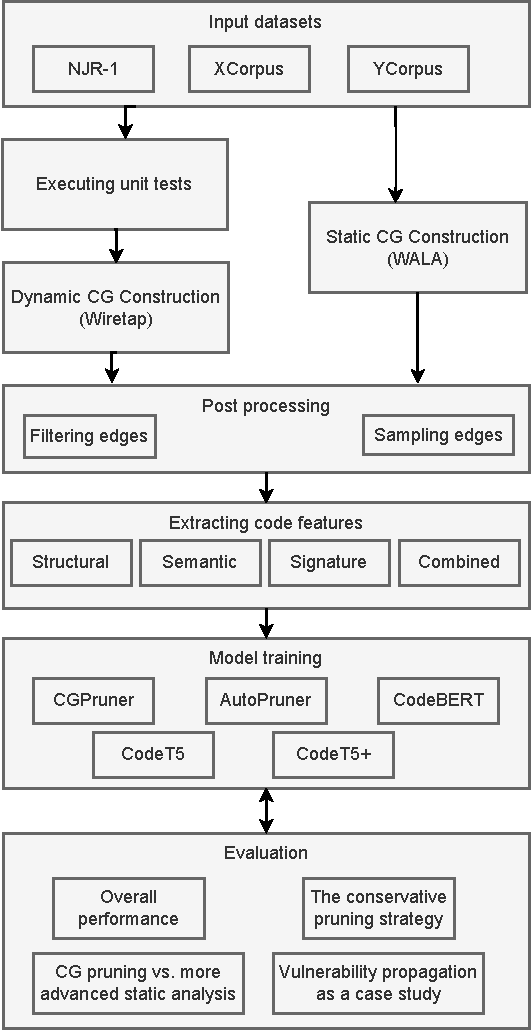
\includegraphics[width=.4\linewidth]{chapters/ch1/figs/overall-study.pdf}
 \caption{Overview of our approach used in this study}
 \label{fig:overall}
\end{figure}

\subsection{Datasets}\label{subsec:datasets}
In this section, we describe the three datasets of our study, that we use to train and evaluate the ML-based CG pruning models.

\paragraph{NJR-1}
Normalized Java Resource (NJR)~\cite{palsberg2018njr} is an infrastructure to leverage the potential of Big Code. The normalization enables searchability, scriptability, and reproducibility. The NJR comprises 100,000 executable Java programs, a set of pre-existing tools, which facilitate the development of novel research tools. For evaluating the ML-based call graph pruning models, we use a subset of the NJR1 dataset, created by the work of Utture et al.~\cite{utture2022striking}. The subset contains 141 programs from the NJR-1 benchmark suite, of which 100 programs are used for training the models and 41 programs for evaluation. The selection of 141 programs from NJR-1 programs was based on criteria such as each program having at least 1,000 methods and 2,000 static call graph edges as per Wala, executing a minimum of 100 distinct methods during runtime, and exhibiting high coverage, i.e., executing a large portion of the methods that can be reached from the main method (with an average coverage of 68\%). On average, each selected program comprises around 560,000 lines of code, excluding the standard library~\cite{utture2022striking}. 

\paragraph{XCorpus}
The XCorpus dataset~\cite{dietrich2017xcorpus} contains a set of 76 executable Java programs, which includes 70 from the Qualitas Corpus~\cite{tempero2010qualitas}. This corpus combines both built-in and generated test cases, offering better branch coverage than the DaCapo benchmark~\cite{blackburn2006dacapo}. While the DaCapo benchmark and Qualitas Corpus are curated datasets for benchmarking and static analysis, respectively, XCorpus combines the strengths of both—being executable (like DaCapo) and diverse and extensive (like Qualitas Corpus). Such a dataset is useful for research on program analysis, studies combining static and dynamic analyses, or studies on program transformations that evaluate impact through program execution pre- and post-transformation. The average coverage for XCorpus' programs is moderate, with 62.35\% for built-in and 60.25\% for
generated tests by Evosuite~\cite{fraser2011evosuite}. On average, each program has an average of around 36K lines of code. XCorpus has been used in the empirical studies on the soundness of Java call graphs~\cite{sui2020recall, reif2019judge}.

\paragraph{YCorpus}
For this work, we created a new dataset, namely, YCorpus, based on an existing dataset used in a recent empirical study by Khatami and Zaidman~\cite{khatami2023state}, which investigates state-of-the-practice in quality assurance in Java-based open source software development. Specifically, they have studied 1,454 popular Java projects on GitHub with more than 100 stars. Given this, we selected 40 Java projects with the criteria that each project has higher than 80\% test coverage. These 40 projects have 88\% test coverage on average, which is substantially higher than that of XCorpus and NJR-1.
Also, YCorpus contains real-world Java projects such as Apache Commons IO, AssertJ, and MyBatis 3, and each project has an average of around 50K lines of code.
Both XCorpus and YCorpus have been reduced to the programs that we could build and for which we were able to construct both static and dynamic CGs.

\paragraph{NYXCorpus}
In the remainder of the paper, we will refer to NYXCorpus as a dataset to indicate that we have based our experiments on the joined data of all three corpora.

\paragraph{Source Code Recovery}
The original NJR-1 dataset lacks source code for the dependencies of its programs.
However, call graphs contain nodes/methods related to dependencies and code language models need source code to learn the call graph pruning task.
We have identified dependencies in the NJR-1 dataset, located their respective repositories (often on platforms like GitHub), and downloaded the necessary source code to extend the dataset with the original code, including comments, for deeper code understanding.
For XCorpus and YCorpus, we downloaded sources JARs for their programs via the Maven or Ant command-line tools.

\subsection{Call-Graph Generation}\label{ch1:subsec:CGG}
This subsection describes our dynamic and static CG generation and explains our filter and sampling criteria for program edges.

\paragraph{Dynamic Call Graphs} 
To evaluate (pruned) static call graphs, we need to establish an "oracle", a known ground truth that represents actual program behavior. In this context, the oracle refers to vertices in a call graph which represents methods. These methods are recognized using a mix of the class name where the method is defined, the method's name, and a descriptor, as per the Java language specification~\cite{lindholm2021java}, to account for overloading. The edges in call graphs are formed by pairs of source and target methods.
To obtain such an oracle, we utilize unit tests that are commonly available and can be an effective way to initiate program executions. In fact, built-in test cases offer a unique insight as they represent the \textit{intended} behavior of a program, mirroring the experience an end-user might have when using the software in a real-world setting~\cite{sui2020recall}.

To collect the method calls of a program, we have instrumented it via Wiretap~\cite{kalhauge2018sound}, a tool to trace information from a running Java program. Specifically, we wrote a recorder to insert probes at Java method entries and exits to record call relationships.
We then ran all available unit tests to gather execution paths, creating dynamic call graphs for the actual execution paths, serving as an oracle or "ground truth" for evaluating ML-based call graph models.
We use this \emph{dynamic} data to train a model for detecting and pruning irrelevant or infeasible paths in \emph{static} CGs.

\paragraph{Static Call Graphs}
We employ the WALA framework~\cite{fink2012wala} to generate static CGs using both context-insensitive and context-sensitive control flow analysis (CFA). Control flow analysis is essential for understanding how functions call each other in a program and this is required for program analysis and optimization. Specifically, we use \emph{context-insensitive} 0-CFA (Zeroth-order Control Flow Analysis)~\cite{shivers1991control}, which creates call graphs by tracking function calls without considering their calling context or parameter values, providing a basic but imprecise approximation of runtime behavior. We also employ the \emph{context-sensitive} 1-CFA algorithm, which improves precision by distinguishing function calls based on their most recent calling context, allowing for more accurate interprocedural analysis than 0-CFA~\cite{shivers1991control}. However, the improvement in precision comes at a computational cost, as 1-CFA requires significantly more resources and time to analyze programs compared to 0-CFA.

For this study, we chose WALA over alternatives like DOOP~\cite{smaragdakis2021doop} and Soot~\cite{vallee2010soot} as it has better support for Java language features such as lambda expressions and, as of this writing, it supports Java bytecode up to JDK 17~\cite{wala}. We follow prior research work~\cite{utture2022striking, le2022autopruner} and do not use WALA's handler for Java reflection, which can potentially miss some execution paths that involve reflective calls. In short, given a Java program, we perform the following steps to construct a static CG using the WALA framework:

\begin{itemize}
    \item We consider each project's main JAR file as the application scope and its transitive dependencies as the extension scope.
    \item We perform a \emph{Class Hierarchy Analysis}~\cite{dean1995optimization}, which involves constructing the class inheritance hierarchy to facilitate the resolution of method call targets.
    \item All non-private methods within all public classes are used as entry points for WALA's call graph builder.
    \item The obtained entry points and the CHA structure are used to construct 0/1-CFA static CGs.
\end{itemize}

\paragraph{Filtering edges} Considering the call graph pruning problem, we are interested in call graph edges related to the application itself and its dependencies.
We follow previous work and opt for removing edges to/from the Java standard library as its enormous size would dominate the dataset and skew the evaluation~\cite{utture2022striking}.
Specifically, we remove all call edges that start with the following prefixes: 
\code{java/}, \code{javax/}, \code{sun/}, \code{com/sun/}, \code{jdk/}.

\paragraph{Large Programs} Utture et al.~\cite{utture2022striking} observed that a few programs in the NJR-1 dataset have a very large number of call-graph edges (over 20K), and they randomly sampled 20K edges from the edge sets of those programs. Following this, we also randomly sampled 20K edges from the edge sets of 5 programs in the XCorpus and YCorpus datasets to alleviate the skewness in the dataset distribution. This also prevents bias towards large programs when training a model/classifier. Also, we do not remove or sample edges where they exist in both dynamic and static call graphs, as fewer of these true edges exist.
A removal of true edges would harm the performance of the ML models at retaining true edges, i.e., recall.

\subsection{Call-Graph Pruning Models}\label{ch1:sec:models}
In this subsection, we describe several machine learning techniques, including code language models, which we extend and employ for our CG pruning task.

\paragraph{Random Forest~\cite{ho1995random}} An ensemble learning method, constructs decision trees on bootstrapped datasets using Bagging~\cite{breiman1996bagging}, considering a random feature subset at each node. Predictions are derived from majority voting for classification or averaging for regression tasks. The algorithm is versatile and adept at handling numerous inputs, missing values, and errors in unbalanced datasets. However, it can be a "black box" model and may overfit noisy datasets.

\paragraph{CodeBERT~\cite{feng2020codebert}} A bimodal pre-trained model for programming language (PL) and natural language (NL) tasks, leverages a Trans\-former-based architecture~\cite{vaswani2017attention} and a hybrid objective function inclusive of replaced token detection during pre-training. It utilizes both bimodal and unimodal data, helping to learn better generators. Trained on CodeSearchNet~\cite{husain2019codesearchnet}, which contains GitHub repositories in six languages, it is similar to multilingual BERT without explicit language markers. Empirical results show that fined-tuned CodeBERT has superior performance on natural language code search and code documentation generation tasks. Without parameter fine-tuning, zero-shot setting tests also indicate the superiority of RoBERTa~\cite{liu2019roberta}, suggesting its effective learning and application in NL-PL tasks. CodeBERT has a parameter size of 125M.

\paragraph{CodeT5~\cite{wang2021codet5}} Built on the T5 architecture~\cite{raffel2020exploring}, utilizes denoising sequence-to-sequence pre-training for both understanding and generation tasks in natural language. A novel identifier-aware pre-training task is introduced for better leveraging code semantics. Similar to CodeBERT, it is pre-trained on CodeSearchNet~\cite{husain2019codesearchnet} data and additional data from open-source GitHub  C/C\# repositories. It is fine-tuned on most CodeXGLUE benchmark tasks and supports multi-task learning. Experimental results reveal that CodeT5 outperforms CodeBERT on various tasks, demonstrating enhanced capture of semantic information from code. The CodeT5 base model has a parameter size of 220M.

\paragraph{CodeT5+~\cite{wang2023codet5+}} An adaptable family of encoder-decoder Large Language Models (LLMs) designed for code tasks, combining different pre-training objectives, including span denoising, contrastive learning, text-code matching, and causal language modeling, for flexible applications in various modes. Initiated with frozen off-the-shelf LLMs~\cite{nijkamp2022codegen}, it circumvents training from scratch, promoting efficient scaling. Upon evaluating 20+ code-related benchmarks, CodeT5+ exhibits superior performance in tasks including code generation, completion, and text-to-code retrieval. The CodeT5+ base model has a parameter size of 770M.

\subsection{Code Features}\label{ch1:sec:feat}
We use the following features or code representations to train our ML-based CG pruning models.
The intuition behind all features is to provide information about the usefulness of an edge.

% NOTE: We don't use this table to save space in the paper.
% \begin{table}
% \centering
% \caption{Structural features for pruning call graphs}
% \vspace{-6pt}
% \begin{tabular}{@{}ll@{}}
% \toprule
% \textbf{Feature} & \textbf{Description} \\ 
% \midrule
% % \small
% src-node-in-deg & number of edges ending in caller \\
% src-node-out-deg & number of edges out of caller \\
% dest-node-in-deg & number of edges ending in callee \\
% dest-node-out-deg & number of edges out of callee \\
% depth & length of shortest path from main to caller \\
% repeated-edges & number of edges from caller to callee \\
% L-fanout & number of edges from the same call-site \\
% node-count & number of nodes in call graph \\
% edge-count & number of edges in call graph \\
% avg-degree & average src-node-out-deg in call graph \\
% avg-L-fanout & average L-fanout value in call graph \\
% \bottomrule
% \end{tabular}
% \label{tab:struct-feat}
% \end{table}

\paragraph{Structural}
Utture et al. \cite{utture2022striking} engineered a set of structural features encapsulating vital contextual and semantic call edge details, adhering to three criteria: linear-time computational complexity, interpretability/generalizability, and black-box nature. The proposed feature set is a combination of local and global information extracted from static call graphs (more info in~\cite{utture2022striking}). The structural features, $f_{struct}$, build a $k_{s}$-dimensional vector ($k_{s}=11$):
\begin{equation}
\mathbf{f}_{struct} = [x_{1}^{struct}, x_{2}^{struct}, ..., x_{k_{s}}^{struct}]
\end{equation}

% The proposed feature set for a static call graph edge, shown in Table\ref{tab:struct-feat}, combines local and global details, with the first seven features providing local information and the last four offering global information. 

\paragraph{Semantic}
Semantic features are extracted from the source code of the caller and callee functions, which is also used in the work of Le-Cong et al.~\cite{le2022autopruner}. Unlike hand-crafted structural features, semantic features are automatically learned by using code language models. They can generate a high-dimensional vector that captures the statistical relationships between caller and callee functions. Thus, each edge in the call graph has an associated embedding that represents the semantic relationship between the caller and the callee. Conceptually, semantic features are represented as follows:
\begin{equation}
\small
\texttt{[CLS]} \langle \texttt{caller's source} \rangle \texttt{[SEP]} \langle \texttt{callee's source} \rangle \texttt{[EOS]}
\end{equation}
The semantic features, $f_{sem}$, are represented as a $k_{c}$-dimensional vector ($k_{c} = 768$), which are the output embeddings of a code language model such as CodeT5.
\begin{equation}
\mathbf{f}_{sem} = [x_{1}^{sem}, x_{2}^{sem}, ..., x_{k_{c}}^{sem}]
\end{equation}

\paragraph{Signature-based}
AutoPruner~\cite{le2022autopruner} extracts features from caller and callee method signatures to supplement CG nodes without source code~\cite{apimp}, namely, \emph{class \& method name}, \emph{parameters}, and \emph{return types}.
This code feature provides minimal code context but is helpful when source code is unavailable.
Signature-based features, $f_{sig}$, are represented as a $k_{c}$-dimensional vector:
\begin{equation}
\mathbf{f}_{sig} = [x_{1}^{sig}, x_{2}^{sig}, ..., x_{k_{c}}^{sig}]
\end{equation}

\paragraph{Combined}
Le-Cong et al.~\cite{le2022autopruner} proposed a combined feature set, which takes advantage of both structural and semantic features, to prune call graph edges effectively. It has empirically shown that AutoPruner~\cite{le2022autopruner}, CodeBERT, with the combined feature set, outperforms a RandomForest model trained on structural features. The combined features, $f_{comb}$, are represented as the concatenation of two vectors $\mathbf{x}_{sem}$ and $\mathbf{x}_{struct}$:
\begin{equation}
\mathbf{f}_{comb} = \mathbf{x}_{struct} \oplus \mathbf{x}_{sem}
\end{equation}

\subsection{Model Training}
We fine-tune our code language models %, described in section~\ref{sec:models},
for two epochs. Specifically, only the encoder module of the CLMs is fine-tuned, which generates embedding for code features mentioned in subsection~\ref{ch1:sec:feat}. To speed up training, we utilized mixed precision training with a floating point precision of 16-bit, which effectively reduces the GPU memory consumption without sacrificing the model's performance. We used an initial learning rate of $1 \times 10^{-5}$, which was found to be effective for training such models without causing instability in the learning process~\cite{le2022autopruner}.
We use cross-entropy loss as the loss function, which is suitable for binary classification problems:
%
\begin{equation}\label{eq:cross-entropy}
L(y, \hat{y}) = -\frac{1}{N} \sum_{i=1}^{N} [w_{1} * y_{i} * log(\hat{y}_{i}) + w_{2} * (1-y_{i}) * log(1-\hat{y}_{i})]
\end{equation}
%
Where $L(y, \hat{y})$ is the loss function comparing the true labels $y$ and the predicted labels $\hat{y}$. $N$ is the total number of samples. $w_{1}$ and $w_{2}$ are the weights associated with the positive and negative classes, respectively. This allows us to define pruning strategies like "conservative" by giving a higher weight to the positive class. The conservative strategy prioritizes high recall by maintaining as many edges as possible and only prunes when certain. We study the effect of these weights on pruning call graphs in RQ2.

We used the AdamW optimizer~\cite{loshchilov2017decoupled}, a variant of the Adam optimizer that corrects its weight decay regularization, boosting generalization and controlling over-fitting. A dropout rate of 0.25 was applied to the models' encoder output to prevent overfitting further~\cite{srivastava2014dropout}. Also, we adopted a linear scheduling policy~\cite{goyal2017accurate} with a warmup phase of 100 steps. This method gradually ramps up the learning rate from zero to the specified maximum ($1 \times 10^{-5}$ in this case) during the warmup phase to avoid large gradient updates early in training, thus aiding in better convergence.

\subsection{Model Inference}\label{ch1:subsec:model-inf}
Given a fine-tuned code language model, we prune CG edges as follows. Let \( \mathbf{x} \) be an input to the CLM and the linear neural network (NN) produces raw scores for the two classes, \( z_0 \) and \( z_1 \). Then, the softmax function converts these raw scores into probabilities.% for each class.
\begin{equation}
p(y = i | \mathbf{x}) = \frac{e^{z_i}}{e^{z_0} + e^{z_1}}
\end{equation}
Where \( i \) is the class label which can take values 0 or 1 and $p(y = i | \mathbf{x})$ is the probability of class $i$. Finally, we use a decision function with a threshold (e.g., \( \tau = 0.5 \)) to decide the predicted class as follows.
\begin{equation}\label{eq:decision_func}
\hat{y} = 
\begin{cases} 
1 & \text{if } p(y = 1 | \mathbf{x}) > \tau \\
0 & \text{otherwise}
\end{cases}
\end{equation}
In many cases with NNs having two output neurons, since the probabilities produced by the softmax function for both classes sum to 1, a threshold of 0.5 is commonly used. If \( p(y = 1 | \mathbf{x}) > 0.5 \), it automatically implies \( p(y = 0 | \mathbf{x}) < 0.5 \) and vice versa.

\begin{table}
\centering
\caption{Stats for the datasets used in evaluation}
\label{ch1:tab:data-stats}
\small
\begin{threeparttable}
\begin{tabular}{@{}l rr c rr r@{}}
\toprule
\multirow{2}{*}{\textbf{Dataset}} & \multicolumn{2}{c}{\textbf{Num. Edges}} && \multicolumn{2}{c}{\textbf{Num. Tokens}} & \multirow{2}{*}{\textbf{P/R Ratio}}\tnote{1} \\
\cmidrule{2-3} \cmidrule{5-6}
 & \textbf{Train} & \textbf{Test} && \textbf{Train} & \textbf{Test} & \\
\midrule
NJR-1 & 859K & 405K && 262M & 124M & 18.7 \\
XCorpus & 269K & 57K && 22M & 8M & 2.4 \\
YCorpus & 242K & 72K && 35M & 9M & 3.7 \\
NYXCorpus & 1.37M & 534K && 319M & 141M & 7.6 \\
\bottomrule
\end{tabular}
\begin{tablenotes}
\item[1] Ratio of to-be-pruned and to-be-retained edges.
\end{tablenotes}
\end{threeparttable}
\end{table}

\newpage
\section{Evaluation Setup}\label{ch1:sec:eval-setup}
In this section, we explain the evaluation metrics for evaluating (pruned) call graphs, the implementation details, model training, and the characteristics of the datasets used in this study. 

\paragraph{Evaluation Metrics}\label{ch1:sec:eval-metrics}
Similar to the previous work~\cite{utture2022striking, le2022autopruner}, to assess the accuracy of a static call graph, we use the common evaluation metrics, precision and recall. We denote the edge set generated by a static call-graph constructor as $E_S$, and the edge set created by Wiretap as $E_D$. The proportion of incorrect identifications is represented by (1-Precision). To obtain the average precision and recall values for the complete test set, we calculate the mean precision and recall values of individual programs and the $F_{\beta}$ measure.
%
\begin{align*}
\text{Precision} = \frac{|E_S \cap E_D|}{|E_S|} \quad \quad \text{Recall} = \frac{|E_S \cap E_D|}{|E_D|}
\end{align*}
\begin{equation*}
F_\beta = \frac{(1 + \beta^2) \times Precision \times Recall}{\beta^2 \times Precision + Recall}
% F1-measure = \frac{2 \times Precision \times Recall}{Precision + Recall}
\end{equation*}

where $\beta$ determines the weight of precision in the combined score. $\beta < 1$ gives more weight to precision, while $\beta > 1$ favors recall. We report $F_1$ and $F_2$ in our evaluation.

\paragraph{Implementation and Environmental setup}
To parse and extract Java methods' source code, we utilized a Java parser~\cite{javap}. We used PyTorch 2.0~\cite{paszke2019pytorch, pt2} with PyTorch Lightning 2.0~\cite{ptl2} to train and evaluate code language models described in section~\ref{ch1:sec:models}. We used the pre-trained code language models from HuggingFace's transformers library~\cite{wolf2019huggingface}. To implement the CGPruner model, i.e., RandomForest, we employed the scikit-learn library~\cite{pedregosa2011scikit}. We used NetworKit~\cite{angriman2022}, a toolkit for large-scale network analysis with optimized algorithms to process graph data and extract structural features. We also used JGraphT~\cite{jgrapht} in Java to do graph traversals and reachability analysis. We performed all the experiments on a Linux workstation (Ubuntu 22.04 LTS) with Intel Core i9 13900KS@6GHz, an RTX 4090 24GB, and 2x48GB (96GB) DDR5 RAM.

\paragraph{Datasets characteristics} Table~\ref{ch1:tab:data-stats} shows the characteristics of the NJR-1, XCorpus, and YCorpus datasets. NJR-1 has 1.2M samples/edges, whereas XCorpus and YCorpus have 326K and 314K edges, respectively. We also have a "meta" dataset, namely, \textit{NYXCorpus}, by combining the training and test sets of the three datasets. This allows us to compare the performance of the models across all datasets and their programs.

In Table~\ref{ch1:tab:data-stats}, we also reported the P/R ratio for each dataset, representing the number of to-be-pruned edges divided by the number of true edges. It can be seen that NJR-1 has a P/R ratio of 18.7, which is much higher than that of XCorpus and YCorpus. This means that the NJR-1 dataset is massively imbalanced. For XCorpus and YCorpus, a lower P/R ratio means that more static edges are observed during test execution at run-time. Also, as expected, NYXCorpus is placed between NJR-1 and Y/XCorpus given its P/R ratio.

\section{Evaluation}\label{ch1:sec:eval}
This section presents the motivation, methodology, and empirical results for all research questions that were defined before. 

%%%%%%%%%%%%%%%%%%%%%%%%%%%%%%%%%%%%%%%%%%%%%%
\subsection{\textbf{RQ}$_{1}$: How do ML-based CG pruning models generally perform at a CG pruning task?}
As the first step of our evaluation, we want to explore the overall performance of the different ML models and their capacity to prune static CGs.
This first assessment provides insights into their abilities and allows us to reduce the list to the most promising candidates for the rest of the paper.
 
\paragraph{Methodology} We used our three datasets (NJR-1, XCorpus, and YCorpus) for this experiment.
Specifically, for the NJR-1 dataset, we trained and evaluated the models in the same way prior work did~\cite{utture2022striking}, using 100 programs for training and 41 for evaluation.
For XCorpus/YCorpus, we trained the models on 12/15 programs and evaluated them on 4/3 programs, respectively.
The results also list NYXCorpus, which is a combination of the three datasets that helps us with choosing the overall best-performing models.
For all datasets, Wala's static CGs were constructed using 0-CFA and there is no overlap of programs in the training and test sets. We should also point out that, for the CLMs, we use semantic features if source code is available for an edge/sample. Otherwise, we use the signature-based feature as a fallback.

To find the optimal hyper-parameters for CGPruner (i.e., RandomForest), similar to the work of Utture et al.~\cite{utture2022striking}, we performed 4-fold cross-validation with grid search. In addition to the all models described in subsection~\ref{ch1:sec:models}, we also considered a random binary classifier, which prunes/retains edges with an equal probability, i.e., $0.5$. To assess the quality of pruned static call graphs by the ML models, we used the evaluation metrics described in section~\ref{ch1:sec:eval-setup}.

\begin{table*}
\centering
\caption{Comparison of the models on the NJR-1, XCorpus, YCorpus, and NYXCorpus datasets}
\label{ch1:tab:general-perf}
\resizebox{\columnwidth}{!}{\begin{tabular}{@{}lc@{\quad}c@{\quad}c@{\quad}c@{\quad}c@{\quad}c@{\quad}c@{\quad}c@{\quad}c@{\quad}c@{\quad}c@{\quad}c@{\quad}c@{\quad}c@{\quad}c@{\quad}c@{}}
\toprule
& \multicolumn{4}{c}{\textbf{NJR-1}} & \multicolumn{4}{c}{\textbf{XCorpus}} & \multicolumn{4}{c}{\textbf{YCorpus}} & \multicolumn{4}{c}{\textbf{NYXCorpus}} \\
\cmidrule(lr){2-5} \cmidrule(lr){6-9} \cmidrule(lr){10-13} \cmidrule(lr){14-17}
{\bf Models} & P & R & F1 & F2 & P & R & F1 & F2 & P & R & F1 & F2 & P & R & F1 & F2 \\
\midrule
\textbf{Random Classifier}  & 0.23 & 0.47 & 0.31 & 0.39 & 0.39 & \textbf{0.48} & 0.43 & 0.46 & 0.22 & 0.45 & 0.29 & 0.37 & 0.25 & 0.47 & 0.33 & 0.40 \\       
\textbf{CGPruner}  & \textbf{0.66} & 0.48 & 0.56 & 0.51 & 0.49 & 0.28 & 0.36 & 0.30 & \textbf{0.71} & 0.24 & 0.36 & 0.28 & 0.61 & 0.43 & 0.50 & 0.46 \\
\textbf{AutoPruner}  & 0.62 & 0.66 & 0.64 & 0.65 & 0.53 & 0.41 & 0.46 & 0.43 & 0.50 & \textbf{0.51} & \textbf{0.50} & \textbf{0.51} & 0.60 & \textbf{0.61} & 0.60 & \textbf{0.60} \\
\textbf{CodeBERT}  & 0.62 & 0.68 & 0.65 & 0.67 & 0.52 & 0.47 & \textbf{0.50} & \textbf{0.48} & 0.50 & 0.48 & 0.49 & 0.49 & 0.59 & 0.60 & 0.60 & \textbf{0.60} \\
\textbf{CodeT5}  & 0.65 & 0.69 & \textbf{0.67} & 0.68 & 0.54 & 0.31 & 0.39 & 0.34 & 0.50 & 0.48 & 0.49 & 0.48 & 0.63 & 0.58 & \textbf{0.61} & 0.59 \\
\textbf{CodeT5+}  & 0.63 & \textbf{0.73} & \textbf{0.67} & \textbf{0.70} & \textbf{0.61} & 0.23 & 0.34 & 0.27 & 0.54 & 0.46 & \textbf{0.50} & 0.48 & \textbf{0.65} & 0.57 & \textbf{0.61} & 0.58 \\
\midrule
\textbf{Average} & 0.57 & 0.62 & 0.58 & 0.60 & 0.51 & 0.36 & 0.41 & 0.38 & 0.49 & 0.44 & 0.44 & 0.43 & 0.55 & 0.54 & 0.54 & 0.54 \\
\midrule
\textbf{Wala} & 0.24 & 0.95 & 0.38 & 0.59 & 0.39 & 0.95 & 0.55 & 0.73 & 0.22 & 0.90 & 0.35 & 0.55 & 0.25 & 0.95 & 0.39 & 0.60 \\
\bottomrule
\end{tabular}}
\end{table*}

\paragraph{Results} Table~\ref{ch1:tab:general-perf} shows the general performance of all the models on four datasets, namely, NJR-1, XCorpus, YCorpus, and NYXCorpus.
In addition to the traditional F1 score, we have also included the F2 score in our evaluation, which puts a higher importance on the recall of an approach.
The results show that all the ML models substantially outperform the random classifier across all datasets and all metrics, with the exception of the \emph{recall} in the XCorpus, which seems to be an outlier.
The code language models (i.e., AutoPruner, CodeBERT, and CodeT5(+)) generally perform better than CGPruner at the CG pruning task.
This is expected as the CLMs leverage code semantics whereas CGPruner only relies on structural features.

From Table~\ref{ch1:tab:general-perf}, we also observe that all the models perform better on the NJR-1 dataset compared to XCorpus and YCorpus. This is because both XCorpus and YCorpus contain popular real-world Java projects in contrast to NJR-1, which focused on automation over popularity when selecting Java projects~\cite{palsberg2018njr} and popular projects seem to be more difficult for the models. In addition, the ML models perform best on NYXCorpus after NJR-1 with an F2 score of 0.54.
This score shows that the gained precision comes at the price of a reduced recall when compared to Wala.
While the average F2 score is only 0.54 on NYXCorpus, the best models can match the quality of Wala's 0-CFA analysis.
Based on these results, we decided to use CodeBERT and CodeT5 for the subsequent RQs.
These two models perform better than others concerning the F2 score and they do not require structural features, unlike AutoPruner. Also, they are faster compared to CodeT5+ considering both training and inference.

However, these results also bring two follow-up questions.
First, the comparatively low recall and many missing edges can prove impractical for client analyses.
We will explore the effect of more conservative training and pruning strategies in \RQ{2}.
Second, a context-sensitive CG generator might achieve the same performance gain with better soundness.
As such, we will compare the quality and scalability of the results when using a 1-CFA analysis in \RQ{3}.

\subsection{\textbf{RQ}$_{2}$: Can conservative training/pruning strategies improve the results?}

The three datasets of our evaluation are imbalanced, especially NJR-1, as can be seen from the P/R ratio in Table~\ref{ch1:tab:data-stats}. There are substantially more edges that need to be pruned than edges to be kept.
If both true and false edges are treated equally in the training phase, the ML models will get biased towards pruning.
Indeed, the results of RQ1 have shown that the recall drops significantly, so we will experiment with more conservative strategies during training and pruning to limit the effects of the imbalance.
The goal is to keep as many edges as possible to minimize the false pruning decisions.

\paragraph{Methodology} We use the two most suitable ML-based CGs pruners from \RQ{1}, i.e., CodeBERT and CodeT5, and experiment with two conservative enhancements.
First, we assign a weight $w$ during the learning process to the positive class (i.e., retaining edges) in the cross-entropy loss function (see Equation ~\ref{eq:cross-entropy}) to fine-tune two models separately.
Second, we consider the confidence of the pruning decision and require reaching a configurable threshold $\tau$, before an edge gets pruned.
We investigate the effects in two separate experiments.
In the first experiment, we perform a grid search over the training weights $\{0,6, 0.7, 0.8, 0.9, 0.95, 0.99\}$ to investigate the effect of the weighted loss function.
In the second experiment, we used the unweighted version of the two models that have been used in \RQ{1} already, and performed another grid search over the confidence threshold values $\{0,6, 0.7, 0.8, 0.9, 0.95\}$ in the decision function defined in Equation~\ref{eq:decision_func} to find the best-performing confidence level.
The higher the value of $\tau$, the more conservative we are when pruning CG edges.
Both experiments use 0-CFA-based static CGs.

\paragraph{Results} 
Figure~\ref{ch1:fig:weighting-models} shows the performance of the models while fine-tuning them with different weights to the positive and negative classes. For instance, a weight of $0.70$ to the positive class means that the negative class is given a weight of $0.30$. Overall, for both CodeBERT and CodeT5, we observe that the F2 score increases and precision decreases by giving higher weight to the positive class.

The results suggest that the weights of $0.95$ and $0.99$ are the most interesting configurations.
While the F2 score drops slightly when moving from $0.95$ to $0.99$, it is to be expected that the resulting CG is also larger.
It seems that $0.95$ can be considered as the "sweet spot" to achieve a recall close to Wala's while gaining higher precision. The use case for $0.99$ is the application where soundness is essential, like vulnerability analysis.
In short, with weights given to the classes, it is possible to maintain a relatively high recall while having better precision compared to Wala's static call graphs. 

Figure~\ref{ch1:fig:models-threshold} indicates the performance of the models considering different confidence levels for pruning call graph edges.
It can be seen that the higher the confidence level, the higher the F2 score is, which is expected as the model is more confident when pruning edges.
Overall, it becomes obvious that the differences to the unweighted results in Figure~\ref{ch1:fig:models-threshold} are minimal, and also here, the $0.95$ and $0.99$ levels are the best-performing configurations.
The confidence-based filtering seems to be as effective as using weights in the loss function, while not requiring the additional overhead of fine-tuning.

The similar F2 scores of the original and the pruned CG beg the question of how large the effect of the pruning is in practice.
We will investigate the impact on a client analysis and the performance implication of a substantially reduced CG on runtimes in \RQ{4}.

\NewDocumentCommand{\imgSize}{}{.9\columnwidth}
\begin{figure}[]
    \centering
    \begin{subfigure}[b]{\imgSize}  % Adjust width as needed
        \centering
        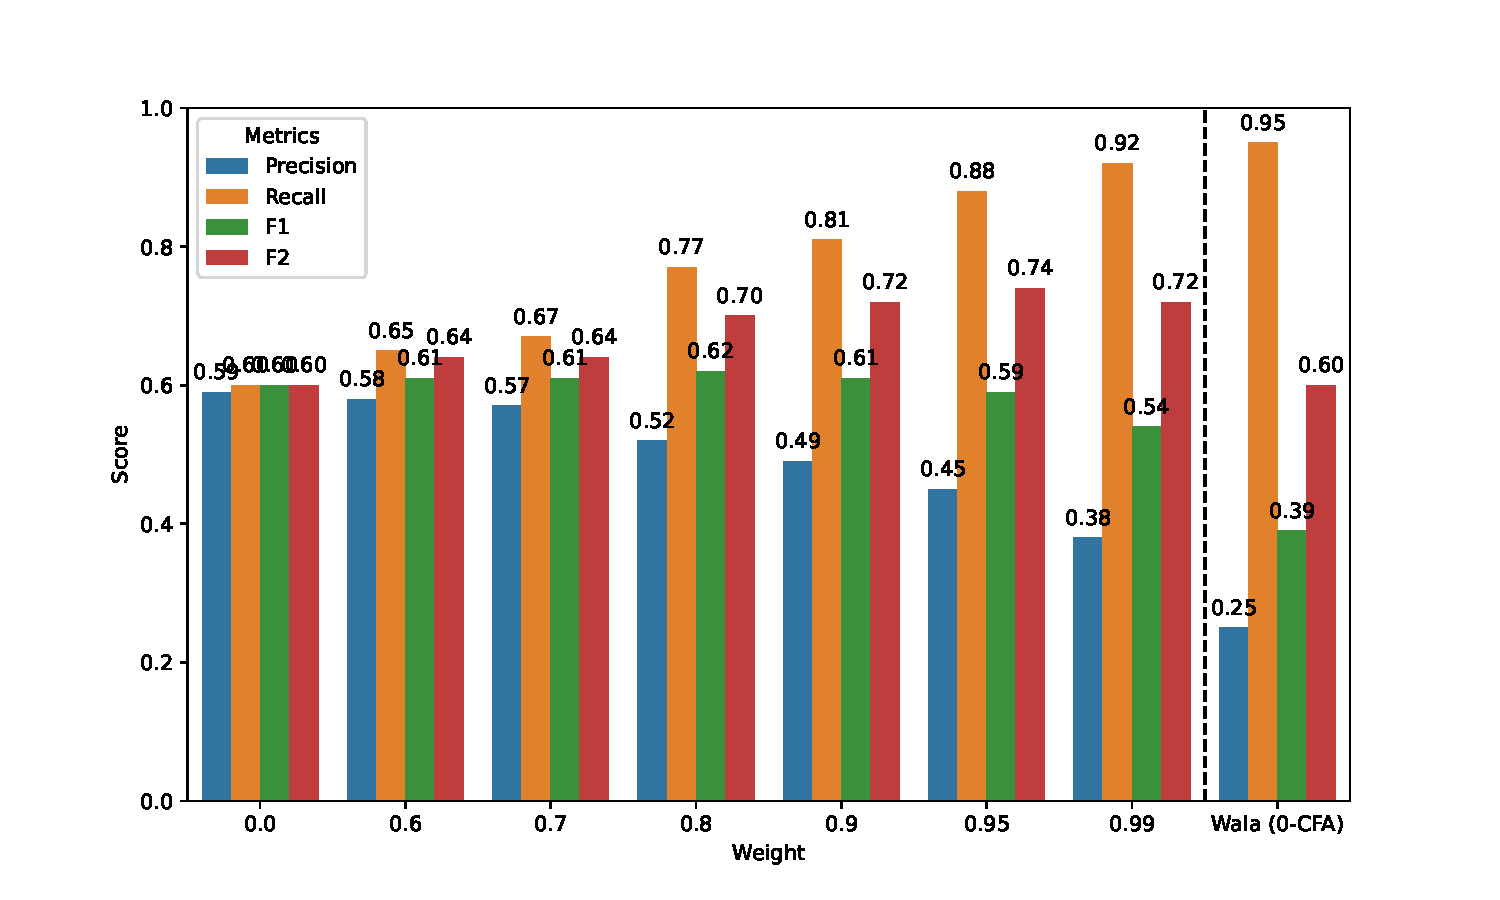
\includegraphics[width=\linewidth]{chapters/ch1/figs/codebert_rq2_fig.pdf}  % \linewidth to fit the subfigure's width
        % \vspace{\imgToCap}  % Uncomment if vertical spacing adjustment is needed
        \caption{CodeBERT}
        \label{ch1:fig:sub1}
    \end{subfigure}
    % Add some vertical space between the figures if needed
    \vspace{1em}  % Adjust the space as needed
    
    \begin{subfigure}[b]{\imgSize}  % Adjust width as needed
        \centering
        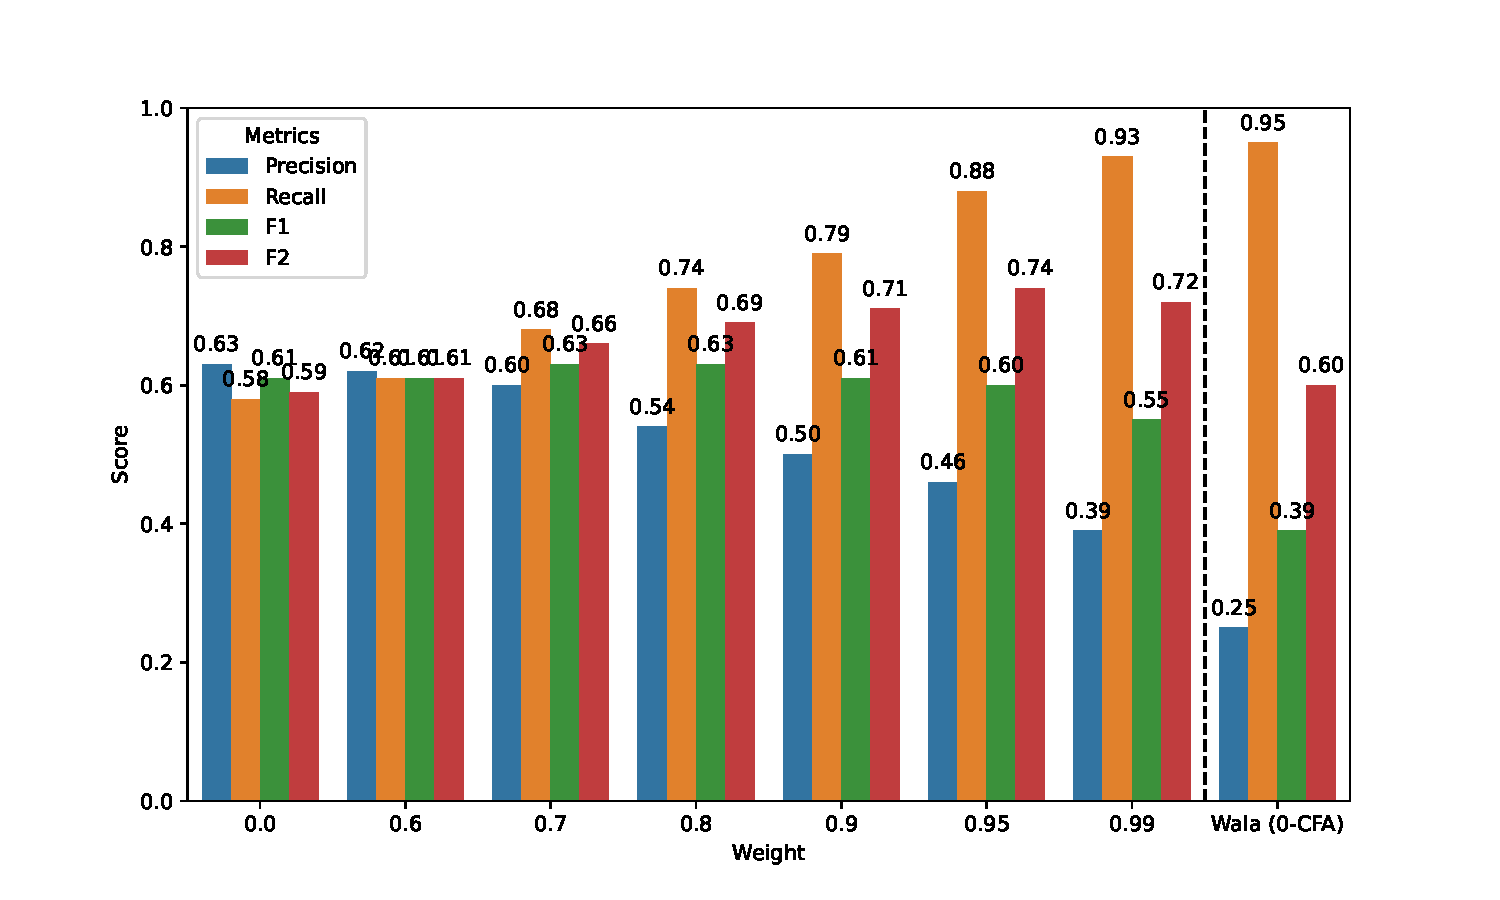
\includegraphics[width=\linewidth]{chapters/ch1/figs/codet5_rq2_fig.pdf}  % \linewidth to fit the subfigure's width
        \caption{CodeT5}
        \label{ch1:fig:sub2}
    \end{subfigure}
    
    \caption{Performance of the models with different weights to the positive class (retaining edges)}
    \label{ch1:fig:weighting-models}
\end{figure}

\begin{figure}
    \begin{subfigure}[b]{\imgSize}
        \centering
        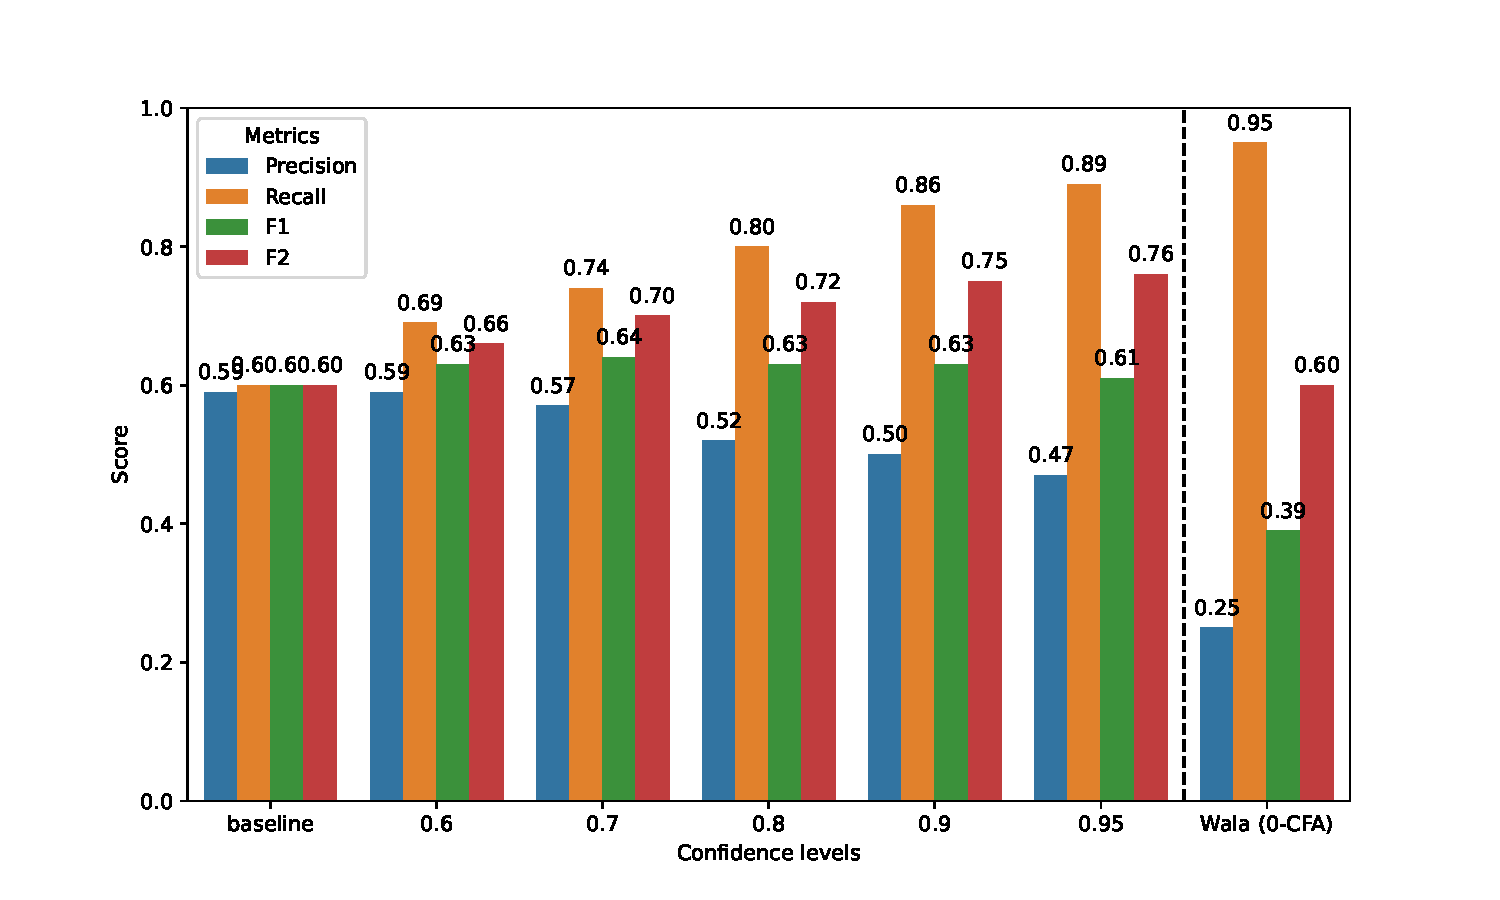
\includegraphics[width=\textwidth]{chapters/ch1/figs/codebert_rq2_1_fig.pdf}
        \caption{CodeBERT}
        \label{ch1:fig:cb-conf-lvl}
    \end{subfigure}
    \vspace{1em}
    
    \begin{subfigure}[b]{\imgSize}
        \centering
        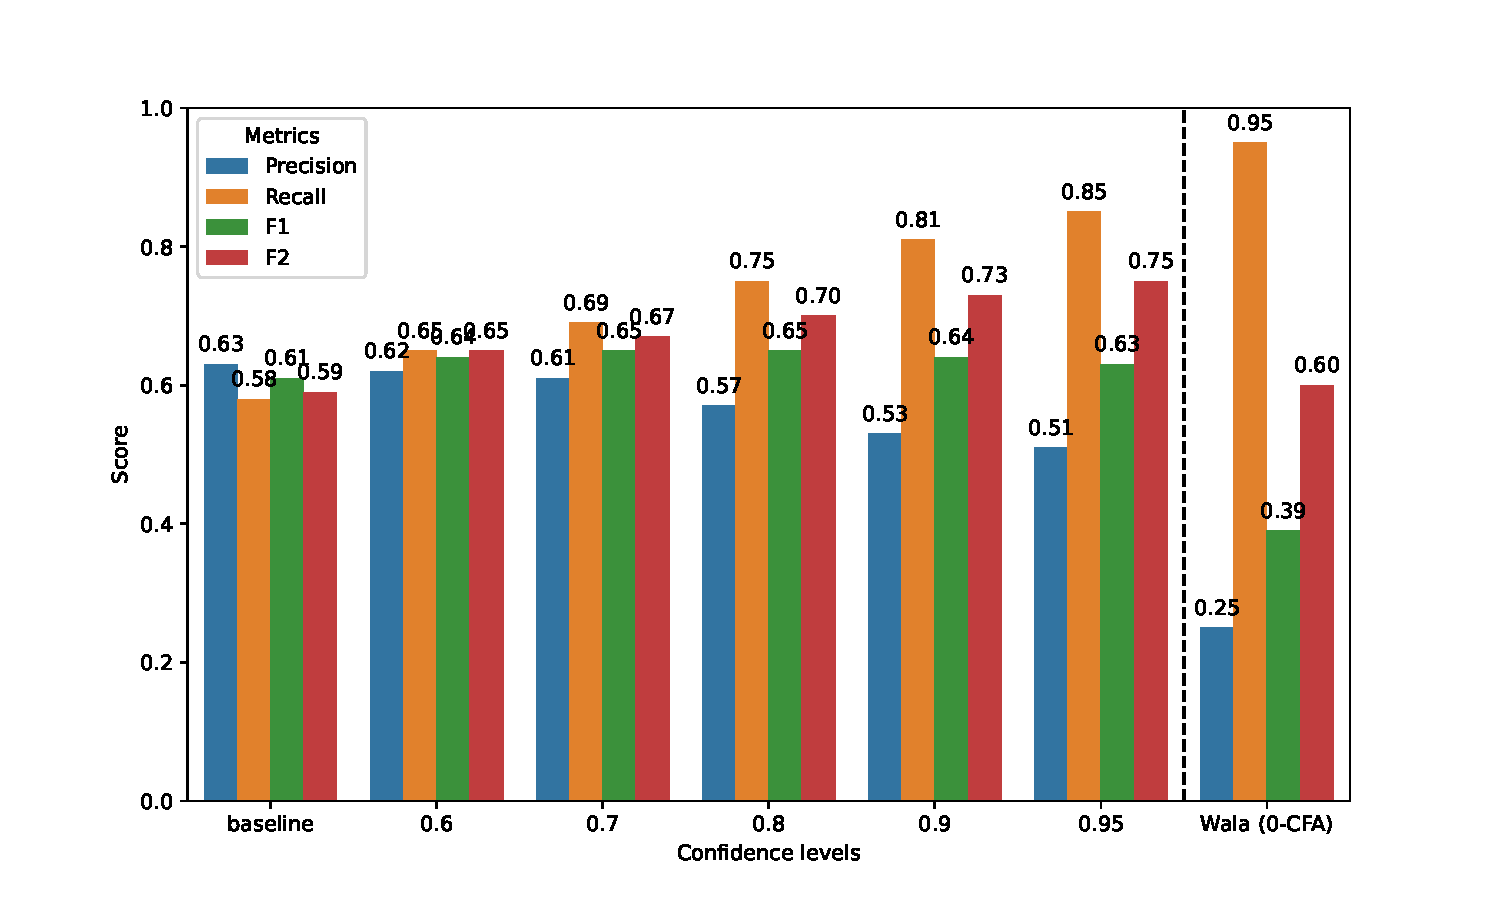
\includegraphics[width=\textwidth]{chapters/ch1/figs/codet5_rq2_1_fig.pdf}
        \caption{CodeT5}
        \label{ch1:fig:models-threshold-t5}
    \end{subfigure}
	
    \caption{Performance of the models by considering different confidence thresholds}
    \label{ch1:fig:models-threshold}
\end{figure}

\subsection{\textbf{RQ}$_{3}$: How do context-sensitive CG generators compare in terms of quality and scalability?}

The results of \RQ{1} have shown that ML-based CG pruning can improve a 0-CFA-based CG with a small computational overhead.
The interesting question is how this overhead compares to running more advanced, context-sensitive CG algorithms like k-CFA (i.e., 1-CFA), which has higher precision but is also computationally more expensive.
In this section, we will investigate how using a 1-CFA analysis in the CG generation compares to 0-CFA (with and without pruning) in terms of performance and scalability.

\paragraph{Methodology}
First, we generate static CGs using both 0-CFA and 1-CFA algorithms for the training and test programs in the NYXCorpus dataset.
We reused the CodeBERT and CodeT5 models that have been fine-tuned on the 0-CFA CGs in \RQ{1}.
We also fine-tuned both CLM models on 1-CFA CGs of the NYXCorpus training set with no weight given to the loss function.
When pruning static CGs, we use a confidence threshold of $0.95$, which we found to be an effective configuration in \RQ{2}.

In our second experiment, we measure the CPU time for generating a static call graph using 0-CFA and 1-CFA. In addition, we show how long it takes to prune call graphs by measuring feature extraction and model inference time separately. Lastly, we sum up the CPU time for both static CG generation and CG pruning to show the total computational time of the whole process.
For each measurement, we report the average and the standard deviation across the NYXCorpus programs. 

\paragraph{Results}
Table~\ref{ch1:tab:0-1cfa-perf} shows the performance of the CodeBERT and CodeT5 models when fine-tuned on 0-CFA and 1-CFA call graphs for the call graph pruning task. The first observation is that, unsurprisingly, Wala's context-sensitive 1-CFA CGs have a 9\% higher precision than Wala's 0-CFA CGs.
Also, the achieved recall is higher, which in combination results in a substantial increase of both F1 and F2 scores by 11\%.
It is interesting to see that this CG improvement is barely visible in the pruned CGs, which only see a 1-2\% improvement in their F1 and F2 scores.

Table~\ref{ch1:tab:run-time-0-1-cfa} provides an overview of the runtimes of the different configurations of 0/1-CFA with and without pruning to allow an assessment of the results in terms of scalability.
CG pruning consists of feature extraction, i.e., tokenizing code sequences and creating semantic features, and model inference, i.e., querying the CLM model to prune call graph edges.
Clearly, the CG pruning task adds additional computational overhead on top of the static CG generation.
The table therefore splits the different stages and shows the averages and standard deviations for static CG generation, feature extraction and inference, and the total runtime in seconds.

The results show that a 1-CFA-based static CG generation takes 42.3s, which is almost twice as long as the 0-CFA algorithm without pruning (21.4s).
The 1-CFA alternative is therefore as expensive as 0-CFA with pruning ($\approx 42$s), however, its standard deviation is much higher (120s vs. 65s).
This is likely caused by the computational complexity of static analysis, which, unlike ML models that have a constant runtime per query, does not scale linearly with the program size.
The results suggest that context-sensitive analysis can be beneficial for small programs, while ML-based approaches scale better.
It is worth noting that the improved CGs of the 1-CFA analysis also have a positive impact on the runtime of the ML approaches.
As the CGs are smaller and contain fewer edges, the runtime of the pruner goes down and deviates less.

\begin{table}[t]
\centering
\caption{Model Performance with 0/1-CFA algorithm}
\label{ch1:tab:0-1cfa-perf}
\begin{tabular}{@{}l@{\quad}c@{\quad}c@{\quad}c@{\quad}c@{}}
\toprule
\multirow{2}{*}{\textbf{Models}} & \multicolumn{4}{c}{\textbf{NYXCorpus}} \\
\cmidrule(lr){2-5}
 & P & R & F1 & F2 \\
\midrule
\multicolumn{5}{@{}l}{\it 0-CFA} \\ 
\midrule
\textbf{CodeBERT}  & 0.47 & 0.89 & 0.61 & \textbf{0.76} \\                                                                
\textbf{CodeT5}  & \textbf{0.51} & 0.85 & \textbf{0.63} & 0.75 \\
\textbf{Wala} & 0.25 & {\bf 0.95} & 0.39 & 0.60 \\
\midrule
\multicolumn{5}{@{}l}{\it 1-CFA} \\ 
\midrule
\textbf{CodeBERT}  & 0.49 & 0.91 & 0.64 & \textbf{0.78} \\                                                                
\textbf{CodeT5}  & \textbf{0.53} & 0.86 & \textbf{0.65} & 0.76 \\
\textbf{Wala} & 0.34 & {\bf 0.97} & 0.50 & 0.71 \\
\bottomrule
\end{tabular}
\end{table}

\begin{table}[t]
\centering
\caption{Runtime of 0/1-CFA algorithms with CG pruning}
\label{ch1:tab:run-time-0-1-cfa}
\begin{tabular}{@{}lccccc@{}}
\toprule
\multirow{2}{*}{\textbf{Models}} & \multirow{2}{*}{\textbf{CG Gen. [s]}} & \multicolumn{2}{c}{\textbf{Pruning [s]}} & \multirow{2}{*}{\textbf{Total Time [s]}} \\
\cmidrule(lr){3-4}
&    & Feature & Infer. &    \\ 
\midrule
\multicolumn{5}{@{}l}{\it 0-CFA} \\ 
\midrule
\textbf{CodeBERT} & \multirow{2}{*}{\mypm{21.4}{57.0}} & \multirow{2}{*}{\mypm{2.8}{3.5}} & \mypm{18.6}{30.9} & \mypm{42.7}{65.2}\\
\textbf{CodeT5} & & & \mypm{18.9}{31.4} & \mypm{43.0}{65.4} \\
\midrule
\multicolumn{5}{@{}l}{\it 1-CFA} \\ 
\midrule
\textbf{CodeBERT} & \multirow{2}{*}{\mypm{42.3}{120.5}} & \multirow{2}{*}{\mypm{1.4}{0.8}} & \mypm{11.7}{11.2} & \mypm{55.1}{122.6} \\
\textbf{CodeT5} & & & \mypm{14.5}{20.0} & \mypm{57.9}{123.9} \\
\bottomrule
\end{tabular}
\end{table}

\subsection{\textbf{RQ}$_{4}$: Is CG pruning practical for a security application like vulnerability analysis?}

All previous experiments have used statistical means to assess the pruning performance of the ML models by comparing ground truth and pruned CG through metrics such as F2-score.
%Retaining high recall, i.e., soundness is essential when using call graphs for critical applications like the analysis of software vulnerabilities.
Previous works have employed client analyses on the pruned CGs, like null pointer exceptions (NPE), to show the effects of the pruning on static analyses in practice~\cite{utture2022striking, le2022autopruner}.
We follow this example and study the effects of CG pruning on vulnerability propagation, a security-sensitive analysis that requires the traversal of call graphs~\cite{mir2023effect}.
We will report on the resulting CG sizes and the runtime of the client analysis.
We expect a significant speed-up in finding vulnerable call paths using pruned static call graphs, though pruned CGs may be susceptible to false negatives, which needs to be investigated.

\paragraph{Methodology} 
We used WALAs 0-CFA static CGs as the baseline and we employ the CodeBERT and CodeT5 models that have been fine-tuned on the training set of NYXCorpus.
We use two configurations for the comparison.
The \emph{conservative} configuration does not add weights to the loss function but uses a $0.95$ confidence threshold.
The \emph{paranoid} configuration reuses the CodeBERT and CodeT5 models that have been fine-tuned with a weight of $0.99$ to the positive class and applies a confidence level of $>0.95$ for pruning.

Our experimental design builds upon the availability of method-level vulnerability information, which is provided by tools like Prospector~\cite{ponta2019msr}.
We did not use real-world vulnerabilities for programs in NYXCorpus though, as the NJR-1 dataset does not include Maven coordinates for its dependencies, plus many projects without vulnerabilities would have to be filtered.
As such, we decided to randomly mark 100 methods as vulnerable in each program of the NYXCorpus test set.
All marked CG nodes represent non-application nodes that are defined in the dependencies of a program.
Our experimental goal is then to measure how long it takes to compute all paths that start in the application and reach a vulnerability with a simple reachability analysis through a Breadth-first-search (BFS).
We calculate the fraction of vulnerable methods that are reachable in a given CG, before and after pruning.
Also, there is no reason to believe that our artificial vulnerabilities are easier to reach than actual vulnerabilities.
To accurately measure the analysis time, we first run the code three times to warm up the JVM and let the JIT compilation do its optimization.
We then compute the reachability another three times and average the required execution time.

It is worth pointing out that while the absolute number of identified paths is lower in a pruned CG, we believe that the crucial information is whether a vulnerable method is reached at all.
Moreover, it is irrelevant for the actionability of the results, whether 1 or 10 affected paths can be found for a given vulnerability.

\begin{table}
\centering
\caption{Vulnerability Propagation Analysis on (pruned) CGs}
\label{ch1:tab:vuln-analysis-results}
\begin{threeparttable}
\begin{tabular}{@{}lrrrrr@{}} % Six columns
\toprule
\multirow{2}{*}{\bf Models} & \multicolumn{2}{c}{\bf CG Size} & \multicolumn{2}{c}{\bf Reachable ...} & \multirow{2}{*}{\bf Time (ms)} \\
\cmidrule(lr){2-3} \cmidrule(lr){4-5}
 & Edges& Nodes\tnote{1} & .. Paths & .. Nodes & \\
\midrule
\textbf{Wala} & 5227.1 & 1420.2 & 853.9 & 99.8\% & \mypm{8.1}{26.6} \\
\midrule
\multicolumn{6}{@{}c@{}}{{\it Conservative Pruning} \hfill ($>0.95$ confidence)} \\ 
\midrule
\textbf{CodeBERT} & 1736.4 & 1048.2 & 515.3 & 86.0\% & \mypm{2.3}{8.1} \\
\textbf{CodeT5} & 1498.2 & 950.5 & 388.6 & 82.0\% & \mypm{1.5}{4.8} \\
\midrule
\multicolumn{6}{@{}c@{}}{{\it Paranoid Pruning} \hfill ($0.99$ weight, $>0.95$ confidence)} \\ 
\midrule
\textbf{CodeBERT} & 3728.4 & 1392.2 & 778.9 & 98.4\% & \mypm{6.6}{23.0} \\
\textbf{CodeT5} & 3503.5 & 1337.3 & 832.5 & 96.9\% & \mypm{6.7}{23.0} \\
\bottomrule
\end{tabular}
\begin{tablenotes}
    \item[1] \#Nodes with at least an incoming and/or out-going edge
\end{tablenotes}
\end{threeparttable}

\end{table}

\paragraph{Results}  
Table~\ref{ch1:tab:vuln-analysis-results} shows the results of vulnerability propagation for both 0-CFA-based static CGs and their pruned version. Note that the reported numbers for CG size, the number of reachable vulnerable paths and nodes are average per test program in NYXCorpus.

WALA is the baseline for the comparison.
It is obvious that both pruning strategies are able to substantially reduce the original CG size from 5.2K edges to 1.5-1.7K ($\approx 33$\%) with the \emph{conservative} setting and 3.5-3.7K ($\approx 69$\%) in the \emph{paranoid} setting.
This results in substantial reductions in the runtime of the client analysis to only 1.5ms (5.4x speedup) in CodeT5 and 2.3ms (3.5x speedup) in CodeBERT.
While the concrete reachability analysis is very fast even on the original CG, we have already seen earlier in the paper that static analyses scale non-linearly, so every reduction in the size of a CG will have a substantial impact in more advanced analyses. 

The substantial reduction of the \emph{conservative} setup comes at the price of only reaching 86\% of the vulnerable nodes.
However, the \emph{paranoid} setup is able to retain the reachability of 96-98\% of the vulnerable nodes, which comes very close to the WALA baseline.
We find that the reduced size and substantial speedup make this result very attractive for large-scale analyses, but the best CG choice always depends on the task and the context.
A security-focused application might accept the slower execution time of an unpruned 1-CFA-based CG analysis to gain a sound result.
For other use cases, a \emph{paranoid} setup might be all that is required, or even a \emph{conservative} analysis could work, when performance is the main issue.
It is noteworthy that, at least in the presented analysis, the pruning does not introduce any false positives and only introduces a small fraction of false negatives. 

\section{Discussion}\label{ch1:sec:discuss}
When reflecting on the obtained evaluation results, we believe that several points are noteworthy and should be considered by researchers and practitioners.

%%%%%%%%%%%
\paragraph{Call graph pruning is an open problem}
As shown throughout the paper, code language models like CodeBERT and CodeT5 have the potential to substantially improve the precision of static CGs.
However, we have also seen that CG pruning is challenging, especially for the real-world programs in the XCorpus and YCorpus.
While the precision is good, the main challenge is achieving a reasonably good recall as well.
The probabilistic nature of CLM models makes it easy to introduce pruning thresholds, however, the parameters of our current approaches must be fine-tuned in a small range at the extremes.
Our models can present a promising step in the right direction, but they do not give an exhaustive answer to the larger problem.
More work is required to find a more robust approach with a more differentiated confidence measure and better results overall.
Future work could explore hybrid approaches that combine heuristic (non-) pruning rules with a CLM model.

%%%%%%%%%%%
\paragraph{Data Imbalance}
We believe that the main limitation that we have faced in our experiments is the massive imbalance of the dataset, as seen in the P/R ratio in Table~\ref{ch1:tab:data-stats}).
Naturally, trained ML models will be biased towards pruning edges rather than retaining them.
We believe that future work should continue to emphasize \emph{recall} over \emph{precision}, as we have done by using the \emph{F2} measure when optimizing their models.
However, this is only the first step and further approaches need to be taken to counter the imbalance.
Our technique for building the ground truth was executing test suites for collecting relevant edges.
Future work could extend this endeavor and trace more extensive program executions and build more complete dynamic CGs.

%%%%%%%%%%%
\paragraph{Hybrid Static Analysis}
Recent works have introduced advancements in ML-based CG pruning, but also advanced program analysis approaches that consider call site sensitivity and more context to improve the precision of static CGs~\cite{ma2023context, jeon2022return}.
Unfortunately, the ML-based approaches and advanced static analyses are still often seen as related, but separate solutions to the CG generation problem.
Likely, because both are very advanced topics in their respective fields and because it is hard to find researchers who are experts in both areas.
We strongly believe though that a hybrid static analysis that integrates ML-based approaches into the static analysis instead of running it as a separate step would be very promising.
Our experiments have shown that even the best static CG generator that we included could not reach 100\% of the vulnerable nodes.
This is, for example, caused by calls through the Java reflection API, which could be suggested through complementing probabilistic approaches.
Another potential combination would be the use of ML to improve the performance of advanced static analyses, which would otherwise not scale to large programs, for example, by accepting unsound results for less important parts of the program.

%%%%%%%%%%%
\paragraph{Feature Engineering}
In contrast to mostly structural features and graph metrics that have been used in previous work, we used semantic features that are based on the source code that surrounds the potential call site.
Overall, we believe that the obtained results are positive, but the feature engineering idea should be investigated more closely.
It is likely that considering full methods for sources and targets exceeds the attention of ML models, therefore important information is not taken into consideration by the model.
Future work could investigate new ways to encode the surrounding context of a method call to find better, semantic features, which might carry more relevant information about the likelihood of a call relation between two methods.

\section{Threats to Validity and Limitations}\label{ch1:sec:ttv}
In this section, we describe the limitations of our work, possible threats to the validity of our empirical findings, and how we address them. We have picked F2 as the main metric to judge the CG quality of our pruned CGs. While it could be possible that the metric still does not emphasize the importance of recall enough, we believe that our results in the vulnerability analysis confirm the suitability of the metric in our experiments.

Our experimental result rests on the ground truth that we have generated through the instrumentation and execution of test suites, which might not be complete or representative of other programs.
We selected programs with a high test coverage, which makes us confident that the results are reliable. Larger benchmark datasets will certainly contain more cases that might be missed in this work, but they would also provide more data to train the ML models.
Overall, we are confident about the representativeness of our data, confirming the data with larger datasets will be left for future work.

We have chosen a vulnerability analysis as a client analysis that is built upon a CG. We do not even start to object that this choice might not be representative of other analysis tasks. However, we think that the generated results and the insights still hold, as the described downsides of static analyses only get worse with larger programs or more advanced static analysis algorithms.

Lastly, we filter call graph edges based on package names as described in subsection~\ref{ch1:subsec:CGG}. This may cause the exclusion of call graph edges related to Graphical User Interface (GUI) components or event-driven programming aspects from the evaluation. This is not a threat but a limitation of the filtering strategy we used, following the previous work~\cite{le2022autopruner, utture2022striking}, which filters such edges if their CG node's URI starts with any of those filtered packages like \texttt{java/}. Future work should propose a more robust approach to filtering call graph edges before the training phase.

\section{Summary}\label{ch1:sec:summary}
This chapter presents an empirical study on the effectiveness of machine learning-based call graph pruning. We identified several key issues in the current state of research on ML-based call graph pruning such as a lack of a suitable benchmark dataset, data imbalance due to static analysis over-approximation, significant recall drop in CG pruning, and no comparison between pruned 0-CFA-based call graphs with context-sensitive algorithms like $k$-CFA.
To address these challenges, we have introduced
(1) the NYXCorpus dataset, combining NJR-1, XCorpus, and YCorpus.
(2) and a conservative strategy to prune CG edges more confidently, which can be tuned by giving weights to classes in the learning process or considering different confidence levels when pruning.
Our empirical findings show substantial improvement in CG precision.
Specifically, ML-based CG pruning can boost precision by 24-34\% while reducing the recall by 2-10\%.
Even though our experiments favor recall over precision, we can show through a comparison with a more advanced 1-CFA-based CG generation that the overall tradeoff is in favor of the ML-based approaches.
We show in a client analysis that by tweaking our model parameters to a \emph{paranoid} setup, it is possible to achieve virtually identical results to a static analysis while being 3.5x faster and operating on a reduced CG with 69\% of its original size.
\chapter{OriginPruner: Leveraging Method Origins for Guided Call Graph Pruning}
\label{ch:origin_pruner}

\NewDocumentCommand\OP{m}{OriginPruner$_{#1}$}

\blfootnote{We are planning to submit this chapter to a software engineering conference by the end of 2024.}

\begin{abstract}
In static program analysis, Call Graphs (CGs) are essential for various tasks, including security vulnerability. Static CGs often suffer from over-approximation to ensure soundness, resulting in inflated sizes and imprecision. Recent research has employed machine learning (ML) models, aiming to prune false edges and enhance CG precision. However, these models have limitations. They require real-world programs with high test coverage to generalize effectively and a lofty inference cost. Motivated by this, in this chapter, we present \tool{OriginPruner}, a novel call graph pruning technique that leverages method origin, which is a method that first introduces a signature within a class hierarchy and is often overridden. Also, by incorporating insights from a localness analysis, finding the scope of method interactions,  into our approach, OriginPruner confidently identifies and prunes edges related to these origin methods.
Our key findings reveal that (1) dominant origin methods, such as \code{Iterator.next}, which significantly impact CG sizes; (2) derivatives of these origin methods are primarily local, enabling safe pruning without affecting downstream inter-procedural analyses; (3) \tool{OriginPruner} achieves a significant reduction in CG size while maintaining the soundness of CGs for security applications like vulnerability propagation analysis; and (4) \tool{OriginPruner} introduces minimal computational overhead. These findings underscore the potential of leveraging domain knowledge about the type system for more effective CG pruning, offering a promising direction for future work in static program analysis.
\end{abstract}

\newpage
\section{Introduction}
In the realm of program analysis, call graphs (CGs) are essential for various tasks, including static program analysis, performance profiling, and security vulnerability assessment.
Call graphs representing function invocations within programs~\cite{ryder1979constructing, callahan1990constructing}.
Creating this representation poses a significant challenge, even for small-scale programs~\cite{ali2012application}, as it is necessary to achieve a balance between \emph{soundness}, i.e., ensuring no legitimate function calls are missed, and \emph{precision}, i.e.,  avoiding the inclusion of superfluous calls.
Despite recent initiatives towards more practical static analyses~\cite{keshani2024frankenstein}, this trade-off is usually decided in favor of soundness, and CGs are typically over-approximated and imprecise~\cite{utture2022striking, antal2023javascript, mir2024effectiveness}.

This leads to a major issue, especially in object-oriented programming languages, where the scalability of CGs suffers from ubiquitous subtyping.
For every call site in a program, a CG generator has to identify all possible target types through a \emph{class-hierarchy analysis}.
For example, a single call to the target method \code{Object.toString} will be expanded by adding several edges to all overridden variants of this method that have been created in subtypes.
This will add a huge \emph{fan out} to every call-graph node that contains such a call, which is a major limiting factor to the scalability of analyses.
As a result, CGs are very big, which affects the performance of downstream static analyses.
Research on static analysis tries to improve the precision by pruning unreachable types, for example, using enhanced pointer analysis based on context-sensitivity or flow-sensitivity~\cite{bravenboer2009strictly, mangal2015user, tan2016making}.
However, such techniques are very computationally expensive even for small improvements~\cite{mir2023effect}.

Recent efforts have introduced novel machine-learning-based pruning techniques that can reduce the size of call graphs by eliminating false edges, e.g., \tool{CGPruner}~\cite{utture2022striking} and \tool{AutoPruner}~\cite{le2022autopruner}.
These approaches learn to prune false CG edges from dynamic traces of actual program executions.
\tool{CGPruner} uses structural features while AutoPruner learns from a combination of structural and semantic features. ML-based CG pruning approaches greatly enhance CG precision by up to 45\%, though they cause a substantial loss in the recall/soundness of call graphs, which renders these approaches impractical for security-focused applications like vulnerability propagation. To alleviate this, very recently, Mir et al.~\cite{mir2023effect} conducted an empirical study on the effectiveness of ML-based CG pruning approaches. Essentially, they proposed a conservative strategy to have a slight loss in recall while benefiting from higher precision. 

While ML-based CG pruning approaches offer promising results, we believe that their quality is conceptually limited by the choice of features that are used to model the CG.
In this chapter, we will approach the pruning problem from a different perspective.
In contrast to existing approaches that are based on basic graph features (like in-degree of a node) or \emph{pseudo-semantic} features (source code as plain text), we propose to base the pruning decision on domain knowledge about the type system.
We will investigate in this chapter, whether a novel CG-pruning approach can use \emph{actual} semantic knowledge about the type system to improve its pruning decisions.
The idea is rooted in \emph{object-oriented programming}, where methods can be overridden in subclasses.
We extract the first definition of each method signature, the \emph{origin method}, and find that, in practice, a small number of origin methods like \code{Object.hashCode} or \code{Iterator.next} are frequently subtyped and used so often throughout typical code bases that they are responsible for a large fraction of the overall CG size.
We believe that instead of investigating general CG pruners, it is more promising to identify and prune only those problematic edges.
We evaluate our intuition through four research questions:
\NewDocumentCommand\rqOneOP{}{Which origin methods impact CG sizes the most?}
\NewDocumentCommand\rqTwoOP{}{How local are the derivatives of the most common origin methods?}
\NewDocumentCommand\rqThreeOP{}{What are the effects of \tool{OriginPruner} on the size and usefulness of CGs?}
\NewDocumentCommand\rqFourOP{}{What is the computational overhead of \tool{OriginPruner}?}

\begin{description}
\item[\RQ{1}] \rqOneOP
\item[\RQ{2}] \rqTwoOP
\item[\RQ{3}] \rqThreeOP
\item[\RQ{4}] \rqFourOP
\end{description}

By answering these research questions, we found several dominating origin methods, most of which are related to the Java object type or the collection API.
%\code{Iterator.next} is the Top-1 most frequent origin method in call graphs and has many unique derivatives.
We found that origin methods are mostly local and seem to be prunable without affecting compatible downstream analyses. % that are based on inter-procedural data flow analyses.
We have implemented a vulnerability propagation analysis as one particular client analysis to investigate the effect of CG pruning on its result.
Using \tool{OriginPruner} we can reduce the CG size by 14-58\%, which translates to a substantial boost in the analysis time of the vulnerability propagation, while only observing a marginal effect on the vulnerability results of vulnerability analysis.
Our results show that an ML-based approach is on par with a simple heuristic, which can be computed much faster, which is a promising direction for future research.

\smallskip
\noindent
Overall, this paper presents the following main contributions:

\begin{itemize}
%
\item We propose a novel CG pruning approach that leverages the method origin.
%
\item We show that the origin methods with the most significant effects on CG sizes are usually local and typically have low effects on inter-procedural analysis, making them a good candidate for pruning.
%
\item Through our evaluation of a vulnerability propagation analysis, we illustrate the need for better feature engineering for ML-based pruning models, as current state-of-the-art pruners cannot outperform a basic pruning heuristic.
%
\end{itemize}

\section{Background}\label{ch2:sec:motive}
Static call graphs build the foundation for many static software analyses.
They represent the calling relationships between methods within a program and model which \emph{source} methods call which \emph{target} methods.
Static analyses can easily extract the \emph{static call sites} from the abstract syntax tree of a program, which represents the locations in which an invocation is supposed to take place.
However, the static call site might refer to an interface type without implementation of that method or during runtime, the target type is a more specific subtype of the static type.
For example, imagine a method with a parameter of type \code{Object}, on which \code{toString} is called, while likely thousands of \code{toString} implementations exist in all loaded classes out of which one will be the actual target of the call in a program run.
The challenge is to identify the set of implemented methods that might be called when the call site is dispatched.
To be sound, a call graph needs to be able to represent all possible executions.
To achieve this, CG generators usually perform a \emph{class-hierarchy analysis} to expand a local call site and include invocations of all known implementations (interface methods) or extensions (overridden methods) that exist throughout the code base and its dependencies.
Naturally, this includes very commonly overridden methods such as \code{Object.toString}.
Including edges for these methods ensures that the call graph accurately reflects all possible method invocations to make the static analysis sound, which is crucial for tasks like impact analysis, optimization, and vulnerability analysis.

\paragraph{Identifying Problematic Methods}
Especially methods that are defined in Java key classes, e.g., in the collection API, have an abundance of implementations in every code base and are used virtually everywhere (e.g., \code{Iterator.next}).
Including all these subtype invocations leads to a significant increase in the size and complexity of the static call graph, potentially making analysis less efficient and more difficult to interpret.

At the same time, most of these basic methods are only used to access data of data structures.
Our intuition says that these methods will be mostly local and that they would not affect static analyses like taint analyses or vulnerability propagation analyses, which follow inter-class data flow.
In this chapter, we explore whether we can automatically identify such problematic methods and whether it is possible to guide CG pruning by starting from only these problematic cases.

\paragraph{Origin Analysis}
While different implementations of the same interface or overridden versions of a method can have completely different method behavior, a good design should be constrained by the \emph{contract} that is established by the first definition of a method signature (i.e., \emph{design by contract}~\cite{meyer2002design}).
We refer to these first declarations as \emph{origin methods}.
As formulated in \emph{Liskov's Substitution Principle}~\cite{LSP}), these origin methods define requirements for subtyping relation.
The principle essentially states that an overridden method must be usable as a drop-in replacement by an unaware caller of the base method, for example, it should not introduce new and unanticipated side-effects or throw \code{Exception} types that clients of the base method do not expect.
In our processing, we will link every method in the dataset to its origin method.

\paragraph{Pruning Call Graphs}
The task of CG pruning is initiated with a static CG denoted as $\mathbb{G}$, a directed graph that is generated via static analysis.
The nodes $V$ within this graph symbolize the defined methods, each distinguished by their method signature that includes the name, parameters, and return type.
The edges $E$ between these nodes are expressed as tuples and mark the invocation of one method (\emph{callee}) by another (\emph{caller}).
%... and the location within the calling function where the invocation occurs (offset).
The CG pruner transforms the set of edges $E^\prime = f_{prune}(E)$ through a pruning function $f$, which uses heuristics or ML-based classifiers to decide on the edges that should be retained.
In this work, we will propose a novel tool that uses information about origin methods to guide the pruning decision.
A refined call graph, $\mathbb{G}^\prime= (V, E^\prime)$, is generated that preserves all vertices, but uses the transformed edge set.

\section{Related Work}
\paragraph{Call Graph Construction}
The study and development of call graphs have been a subject of significant interest. (ML-based) call graph pruning techniques, which do not incorporate real-time data, are categorized under static methods for call graph generation \cite{murphy1998empirical, reif2019judge, sui2020recall}. Conversely, dynamic analysis methods \cite{xie2002empirical, hejderup2018software} have been shown to reduce false positives and improve precision, albeit at the cost of scalability.

Additionally, efforts have been made to enhance the accuracy of call graphs. Lhotak \cite{lhotak2007comparing} introduced an interactive tool designed to elucidate the discrepancies between various static and dynamic analysis tools. Sawin and Rountev \cite{sawin2011assumption} proposed heuristics to better handle dynamic features such as reflection, dynamic class loading, and native method calls in Java. This technique improved the precision of the Class Hierarchy Analysis (CHA) algorithm \cite{dean1995optimization}, while maintaining satisfactory recall rates. Moreover, Zhang and Ryder \cite{zhang2007automatic} focused on producing accurate application-specific call graphs by identifying and eliminating false-positive edges between the standard library and the application itself. Recently, Antal et al.~\cite{antal2023javascript} studied the challenge of generating precise call graphs for JavaScript due to its dynamic nature, and hence they conducted a comparative study of static and dynamic call graph generation tools for JavaScript. They found that while dynamic tools offer perfect precision, the recall of both static and dynamic approaches are very similar, ranging from 58\% to 69\%. Keshani et al. proposed Frankenstein~\cite{keshani2024frankenstein}, a fast and lightweight call graph construction technique for software builds. The main idea is to create partial call graphs for each dependency in a program and then merge the resulting CGs into one whole program CG. Their approach is faster and has a small memory footprint, which makes it suitable for software build systems.

\paragraph{Machine learning for enhancing call graphs}
Currently, there are two notable ML-based models for call graph pruning: CGPruner \cite{utture2022striking} and AutoPruner \cite{le2022autopruner}. Utture et al. introduced CGPruner, an ML-based approach aimed at reducing the false-positive rate of static analysis tools to enhance their appeal to developers \cite{utture2022striking}. CGPruner prunes unnecessary false-positive edges from the static call graph, which is integral to numerous static analyses. This is accomplished through a pre-execution learning process that involves the application of static and dynamic call-graph constructors, with dynamic call graphs utilized solely during the training phase on a set of training programs. This approach notably reduced the false-positive rate, in certain instances, from 73\% to 23\%.

However, CGPruner does not analyze the semantics of the source code. To overcome this shortcoming, Le-Cong et al.~\cite{le2022autopruner} introduced AutoPruner, which aims to eliminate false positives within call graphs by harnessing both the structural and semantic statistical information from the source code of caller and callee functions \cite{le2022autopruner}. AutoPruner employs CodeBERT \cite{feng2020codebert}, a pre-trained Transformer-based model \cite{vaswani2017attention} designed explicitly for code. It fine-tunes this model to discern semantic features of each edge, integrates these with manually crafted structural features, and utilizes a neural classifier to classify each edge as either true or false positive.

Very recently, Mir et al.~\cite{mir2024effectiveness}
has studied the effectiveness of ML-based call pruning and proposed a benchmark dataset, namely NYXCoprus, for this task. Among their findings, they found that CGPruner and AutoPruner produce pruned call graphs with notoriously low recall, which renders these approaches unsuitable for security-focused applications like vulnerability analysis. To alleviate this issue, they introduced a conservative strategy to fine-tune the code language models (CLMs) to maintain a high recall, close to static CGs, and benefit from better precision. This made pruned call graphs produced by CLMs useful for vulnerability analysis while benefiting from faster analysis.

So far, all the discussed papers have tackled the call graph pruning problem with machine learning. There is also a recent work on discovering true edges for JavaScript's call graphs~\cite{bhuiyan2023call}. Their proposed technique combines structural and semantic information and employs Graph Neural Networks (GNNs)~\cite{scarselli2008graph} to identify true edges. The experimental results show a significant improvement to true positive rates in vulnerability detection.

\section{Methodology}

% This figure can be edited at:
% https://drive.google.com/file/d/1el65DoCbC_QntoRRVANquRAtfz9JjPsB/view?usp=sharing
\begin{figure*}
    \centering
    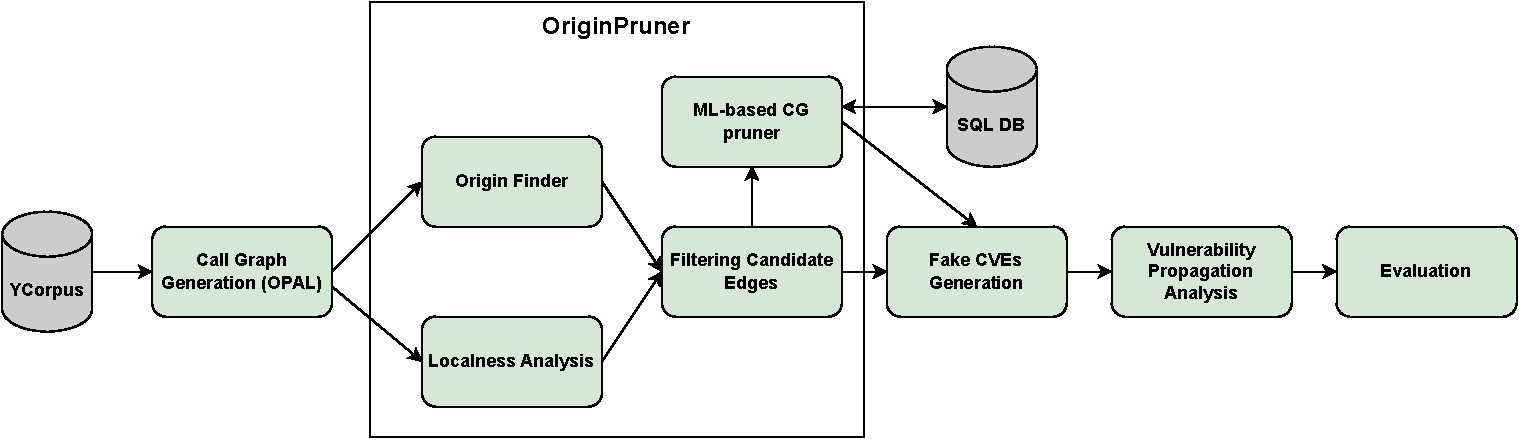
\includegraphics[width=.9\textwidth]{chapters/ch2/figs/overview-cg-pruning.pdf}
    \caption{Overview of our proposed approach}
    \label{ch2:fig:overview}
\end{figure*}

%\subsection{Overview}
Figure~\ref{ch2:fig:overview} shows the overview of our approach. We used Java programs from the YCorpus dataset~\cite{mir2023effect} including their transitive dependencies to feed our pipeline. First, we generate static call graphs as a baseline for our evaluation.
Then, we perform two types of analyses on these call graphs, namely, origin finder and localness analysis. The origin finder identifies places, in which method signatures have been first introduced. The localness analysis then determines how local these methods are, i.e., if the methods rely solely on the Java standard library or use functionalities from methods implemented in the dependencies. Given the results of these two analyses, we identify a set of origin methods that we use as candidates for edge pruning in static CGs.
These candidates get pruned in two different strategies: a simple heuristic exhaustively prunes all calls that are related to these popular origin methods, and a second strategy employs an ML-based CG pruning model to make the pruning decision.
We implement a vulnerability propagation analysis to evaluate the effect of the pruning on the reachability of vulnerabilities.
The following subsections provide more details about the individual steps.

\subsection{Call Graph Generation}\label{ch2:subsec:cg_gen}
To create static call graphs, we employed the OPAL framework~\cite{eichberg2014software, helm2020modular}, an advanced and well-established tool tailored for bytecode analysis. This methodology is based on employing the Class Hierarchy Analysis (CHA) algorithm, renowned for its straightforward yet effective approach to dealing with the complexities inherent in object-oriented programming languages. Specifically, within the OPAL framework, the generation of static call graphs entails a meticulous examination of Java bytecode, aiming to pinpoint potential method invocations. This process culminates in a directed graph, where methods are depicted as nodes, and the possible calls between them are represented as edges. A crucial aspect of this analysis involves scrutinizing not only the application's bytecode but also its transitive dependencies and the Java Runtime Environment (JRE)'s core libraries, particularly the runtime JAR file or \code{rt.jar}. The inclusion of rt.jar is pivotal as it contains the classes necessary to run Java applications, including the standard Java API. By analyzing rt.jar, the framework can construct a more accurate and comprehensive class hierarchy. This hierarchy lays the foundation for resolving virtual method calls, a task achieved by identifying all potential callee methods in light of Java's polymorphism and inheritance mechanisms.
%todo: the following paragraph seems unnecessary
With the consideration of the \code{rt.jar} file, the call graph is enriched with essential runtime context, thereby enhancing the accuracy of identifying and resolving method calls that occur during the actual execution of a Java application. This enriched context is especially beneficial for security vulnerability analysis, as it allows for a more thorough inspection of how an application interacts with the Java standard library, potentially uncovering vulnerabilities that might not be evident through static analysis alone. By integrating the static CGs generated through CHA with insights from Java's runtime environment, we are better positioned to conduct comprehensive security assessments, thereby enhancing the detection and mitigation of security threats.

\subsection{Origin finding}\label{ch2:subsec:origin}
As described in Section~\ref{ch2:sec:motive}, certain methods can cause an "explosion" in the number of edges in call graphs. In this chapter, we define them as "origin methods". They play a pivotal role in understanding and managing the complexity of call graphs in object-oriented programming like Java. These are the methods where a particular method signature is first introduced in a class hierarchy, acting as the root for any subsequent overrides or derivative methods. The concept of origin methods is crucial because it helps identify the source of method signatures that proliferate across subclasses through inheritance and polymorphism. When a method in a superclass is overridden by multiple subclasses, each override is considered a derivative method. This inheritance and overriding mechanism can lead to a significant increase in the number of edges in a call graph, especially for origin methods high up in the type hierarchy with many subclasses. The explosion of edges attributable to these origin methods reflects the potential paths of method invocations, which can be particularly challenging to analyze due to the increased complexity and size of the call graph.

To tackle the challenge posed by origin methods and their derivatives in static analysis, we proposed an algorithm that is designed to identify and assess the impact of these methods on the structure of call graphs. This algorithm, outlined in the provided pseudocode in Algorithm~\ref{ch2:alg:origin}, systematically examines each edge in a call graph to find the origin method responsible for the method invocation represented by the edge. It iterates through the edges of the CG, tracing each target method's type back through its hierarchy until it finds the highest type where the method signature was first declared. By mapping each method to its origin, this approach allows us to investigate the extent to which a single origin method can influence the call graph, quantifying the number of edges it effectively generates. This information is invaluable for optimizing CG analyses, as it highlights the methods that are most influential in the complexity of the graph, guiding efforts to simplify or focus the analysis on the most impactful areas.

The identification of "origin methods" through the aforementioned algorithm enables a systematic way of pruning call graphs, significantly enhancing the efficiency and focus of static analysis. This approach is particularly useful because it allows for the reduction of call graph complexity without substantial loss of essential information. 
%todo: the following sentence doesn't seem right. You prune the unimportant parts of CG based on the origin analysis but here it seems you say the security analysis should focus on origins and derivatives.
For instance, in scenarios where the analysis aims to identify potential security vulnerabilities or performance bottlenecks, focusing on the most impactful parts of the call graph, the origin methods, and their immediate derivatives can yield quicker, more relevant insights. 
Pruning based on origin methods systematically reduces the graph's size, making it more manageable and easier to navigate, while preserving the integrity of the analysis by maintaining the critical paths of method invocations. This methodological pruning, therefore, enhances the practicality of static analysis tools, making them more adaptable to large-scale software projects where unpruned call graphs could become impractical to work with.

\begin{algorithm}
\caption{Finding origin methods of a call graph} \label{ch2:alg:origin}
\begin{algorithmic}[1]
\footnotesize
\Function{findOrigins}{$CG$}
    \State $origins \gets emptyMapOfOrigins()$
    \ForAll {$edge_i \in CG.edges()$}
        \State{$target \gets edge_i.target()$}
        \State{$target_{type} \gets target.type()$}
        \ForAll{$parent_{type} \in target_{type}.parents()$}
            \If{$parent_{type}.isFirstDeclare(target.signature())$} 
                \State{$origins.put(target, parent_{type})$}
            \EndIf 
        \EndFor
    \EndFor
    
    \State \Return $origins$
\EndFunction
\end{algorithmic}
\end{algorithm}

\subsection{Identifying Localness Levels}\label{ch2:subsec:localness}
The concept of localness in relation to the derivatives of an origin method introduces a nuanced framework for analyzing the scope and impact of method invocations within an application. This framework categorizes methods based on the extent of their interactions with other components of the system, ranging from purely internal functionality to interactions that cross package boundaries. To this end, we define four categories of localness:

\begin{itemize}
    \item \emph{Level 0}: A method does not call anything or it only calls Java functionalities.
    \item \emph{Level 1}: A method does call other functionalities than Java but it does not exit its class or its class hierarchy.
    \item \emph{Level 2}: A method calls at least one function from outside of its class hierarchy, but it remains within the same project.
    \item \emph{Level 3}: A method calls at least one function from outside of its class hierarchy and the target of this call is also in another package.
\end{itemize}

By labeling the target methods within a call graph with these localness levels, it helps to better understand an application's architecture and the dependencies between its components. For instance, a derivative method with a localness level of 0 or 1 indicates a high degree of cohesion within the class or class hierarchy, suggesting that the functionality is tightly integrated and likely easier to maintain. On the other hand, a derivative with a localness level of 3 points to a broader scope of interaction, which might be necessary for the application's functionality but also introduces more dependencies,
%todo is it necessary to mention maintenance and testing here? Our goal is something else. Instead, if we talk about vulnerability analysis and the fact that local methods do not end up in a vulnerable dependency that would be more helpful
potentially increasing the complexity of maintenance and testing. Algorithm \ref{ch2:alg:categorize} shows how to find the localness level of target methods in call graphs.

\begin{algorithm}
\caption{Localness algorithm}
\label{ch2:alg:categorize}
\begin{algorithmic}[1]
\footnotesize
\Function{Categorize}{$method, CG$}
    \State $label \gets 0$
    \If{isDefinedInJava(method)}
        \State{\Return{$label$}}
    \EndIf
    \ForAll{$ edge_i \in CG.outgoingEdgesOf(method)$}
        \State{$ target_i \gets edge_i.target()$}
        \If{$!isDefinedInJava(target_i) $}
            \If{$ label<2 \And inSameHierarchy(method, target_i)$}
                \State{$label \gets 1$}
            \Else
                \If{$areInSameProject(method, target_i)$}
                    \State{$label \gets 2$}
                \Else
                    \State{$label \gets 3$}
                    \State \textbf{break}
                \EndIf
            \EndIf
        \EndIf
    \EndFor
    \State{\Return{$label$}}
\EndFunction
\end{algorithmic}
\end{algorithm}

\subsection{Pruning Strategy}
After performing the origin-finding analysis, we have the origin methods and their derivatives for Java programs. These methods are frequently overridden or extended across different classes and packages within programs in the dataset. By considering Top-$n$ most frequent origin methods, we create an "exclusion list" of $n$ elements. Given this, we prune call graphs edges for which their target type is a derivative of an origin method in the list. Algorithm~\ref{ch2:alg:prune_cg} shows pseudo-code for pruning call graph edges using the described pruning strategy.

\begin{algorithm}[t]
\caption{Pruning call graphs with a pruning strategy} \label{ch2:alg:prune_cg}
\begin{algorithmic}[1]
\footnotesize
\Function{PruneCG}{$CG, exclusionList$}
    \State $pcg \gets new DirectedGraph()$ 
    \ForAll {$callSite \in CG.getCallSites()$}
        \State $source \gets callSite.getSource()$
        \State $target \gets callSite.getTarget()$
        \State $targetType \gets callSite.getTargetType()$
        \State $excludedTypes \gets exclusionList.get(targetType.getSignature())$
        \If {$NotInExcludedTypes(ExcludedTypes, targetType)$}
            \Comment{The ML-based model is queried here for this edge if using the selective approach}
            \State $pcg.addEdge(source, target)$
        \EndIf
    \EndFor
    \State \Return{$pcg$}
\EndFunction

\Function{NotInExcludedTypes}{$exclsuionList, targetType$}
    \ForAll {$type \in excludedTypes$}
        \If {$type.hasChild(targetType)$}
            \State \Return{False}
        \EndIf
    \EndFor
    \State \Return{True}
\EndFunction
\end{algorithmic}
\end{algorithm}

\subsection{Dataset}
For this work, we used the YCorpus dataset, which was created by Mir et al.~\cite{mir2024effectiveness}. It has 23 Java projects with the criteria that each project has higher than 80\% test coverage. Its programs contain the JARs of transitive dependencies plus source code. Despite its small size, YCorpus is suitable for evaluating (ML-based) call-pruning models, as it contains real-world Java projects such as Apache Commons IO, AssertJ, and MyBatis 3, and each project has an average of around 50K lines of code.

\subsection{ML-based call graph pruning}
ML-based call graph pruning aims to prune superfluous or false edges in static call graphs by learning from actual program execution paths, i.e., dynamic call graphs. For this work, specifically, we employ a well-known code language model, CodeBERT~\cite{feng2020codebert}, which leverages semantics embedded within code. We use the ultra-conservative strategy introduced in the work of Mir et al.~\cite{mir2023effect}, known as "paranoid pruning", which particularly uses a weight of 0.95 in the learning process and a confidence level of over 95\%. This method prioritizes the retention of edges, i.e., very cautiously pruning only when there is high confidence, thus minimizing the risk of losing true call graph edges. With the described strategy, CodeBERT not only enhances the precision of call graphs but also maintains high recall, almost identical to that of static call graphs, which is crucial for downstream analyses, such as vulnerability detection at the method level.

We employ the ML-based CG pruner in combination with our proposed approach, which leverages the results of the origin finder and localness analysis to prune edges. Specifically, we query the ML model to decide whether a candidate edge for pruning, i.e., a 
derivative of the origin methods, should be pruned. We expect that this makes our approach more conservative. In the paper, we refer to this combination as \tool{OriginPruner} with Selective, ML-based pruning.

\subsection{Generating Artificial Vulnerabilities}
To study the effect of our proposed call graph pruning on vulnerability propagation, we follow the methodology of previous work and create artificial CVEs to make the evaluation more scalable~\cite{mir2023effect}. We first separate application nodes from those of dependencies in the whole-program static call graph. This distinction is crucial since the aim is to inject vulnerabilities exclusively into the dependency nodes. We randomly mark 100 of these dependency nodes to be associated with one of the artificial vulnerabilities. The selection should be random to ensure that the simulated vulnerabilities are spread unpredictably across the dependencies, mirroring the nature of real-world vulnerabilities.

\subsection{Vulnerability Propagation Analysis}\label{ch2:subsec:vpa}
To find whether vulnerable nodes/methods in static call graphs are reachable from the main application's methods, we perform an inverse Breadth-First Search (BFS) from nodes identified as vulnerable in the project's dependencies. This analysis has two main advantages. First, it is much faster than performing BFS from application nodes to vulnerable nodes. Because we already know the vulnerable nodes in the call graph and hence we initiate the search from these nodes rather than from all applications nodes. Second, we can pinpoint the sequences of calls that might expose the application to risks emanating from its dependencies. This is crucial for understanding the impact of vulnerabilities in third-party libraries and enabling developers to prioritize and remediate threats more effectively.

\subsection{Implementation}
We implemented most of the components in our proposed approach in Java 11 such as CG generation, origin finding, localness categorization, vulnerability analysis, and artificial CVEs generation. We used Apache Kafka to stream data into our end-to-end pipeline. We employed the JGraphT framework~\cite{jgrapht} to work with graphs and implement vulnerability propagation analysis. Also, we implemented an ML-based CG pruner, a fine-tuned CodeBERT, as an inference service in Python 3.10 using PyTorch 2.2~\cite{pt2,paszke2019pytorch} and Ray Serve~\cite{moritz2018ray}. We used the PostgreSQL database to cache the predictions of the inference service. This is helpful to speed up the ML-based CG pruning process when we consider different sizes of filters in our experiments.

We conducted all the experiments in this chapter on a workstation machine with Ubuntu 22.04 LTS, 2xAMD EPYC 7H12 64-core processor, and 512 GB of RAM. The ML-based CG pruner model inference was done on an RTX 3080 10 GB.

\section{Results}
\subsection{\textbf{RQ1}: Which origin methods impact CG sizes the most?}
We study the origin methods in call graphs as they can provide insights to better understand the complexity of Java applications. Fundamentally, origin methods introduce a method signature subsequently overridden by derivative methods across various types. In other words, the proliferation of derivative methods from a single origin can dramatically increase the complexity of call graphs, which map the interactions and dependencies between different parts of a software system. This complexity is not merely a research problem but also has practical implications for software maintenance, optimization, and vulnerability analysis. By studying the impact of origin methods on the expansion of call graphs, we can identify patterns and anomalies that help us to form a set of heuristics or rules for pruning call graph edges.

\paragraph{Methodology}
To find origin methods in the YCorpus dataset, we first generate static call graphs using OPAL, which is explained in Section~\ref{ch2:subsec:cg_gen}. By iterating through the edges of the generated static CGs, we follow the origin-finding procedure to find the origin of target nodes. We aggregate each project's discovered origin methods to report the Top-10 origin methods in the dataset. In addition, we report the number of unique derivatives for the Top-10 origin methods.

\paragraph{Results}
Table~\ref{ch2:tab:origin_freq} shows the Top-10 most frequent origin methods for YCorpus. \code{Iterator.next()} is the most common origin method with over 15M frequency, which is used to iterate over elements in data structures like \code{Set}, \code{List}, etc. Considering this, our intuition in Section~\ref{ch2:sec:motive} is backed up, providing that methods like \code{toString()} or \code{next()} are very frequent in static call graphs. Moreover, it can be observed that \code{XWrapperBase.toString()} is the 8th most common origin method, which is part of Java Runtime Environment (JRE) and is used for building graphical user interfaces, particularly for X11 windowing systems. As described in Section~\ref{ch2:subsec:cg_gen}, we included JRE libraries when building static call graphs.

Also, Table~\ref{ch2:tab:origin_der} shows the number of unique derivatives for the Top-10 frequent origin methods. Interestingly, \code{Iterator.next()} does not have the most unique derivates given that it is the most common origin method in the YCorpus dataset. In fact, \code{PrivilegedAction.run()} has the most unique derivatives among other origin methods. Overriding this method allows developers to encapsulate security-sensitive operations in a single, reusable component. This can make the code more readable and maintainable, as the security-related code is localized and not scattered throughout the application. Overall, considering the most frequent origin methods and their derivatives, our observation here hints at the fact that these methods can potentially be a candidate for pruning edges in static call graphs. We should also point out that we only reported the Top-10 most common origin methods due to the limited space in the paper. Readers can refer to our replication package for the extensive list.

\begin{table}[!t]
\centering
\caption{Top 10 most common origin methods in YCorpus}
\label{ch2:tab:origin_freq}
\begin{threeparttable}
\begin{tabular}{@{}lr@{}}
\toprule
Method\tnote{a} & Frequency \\
\midrule
% YCorpus
/j.u/Iterator.next()/j.l/Object & 15,795,483 \\
/j.u/Iterator.hasNext()/j.l/BooleanType & 13,691,858 \\
/j.l/Iterable.iterator()/j.u/Iterator & 5,243,680 \\
/j.u/Collection.size()/j.l/IntegerType & 2,317,670 \\
/j.u/Map.get(/j.l/Object)/j.l/Object & 2,274,769 \\
/j.u/Map.put(/j.l/Object,/j.l/Object)/j.l/Object & 1,364,892 \\
/j.u/List.get(/j.l/IntegerType)/j.l/Object & 1,211,656 \\
/s.a.X11/XWrapperBase.toString()/j.l/String & 869,519 \\
/j.u/Collection.contains(/j.l/Object)/j.l/BooleanType & 693,782 \\
/j.u/Enumeration.nextElement()/j.l/Object & 693,372 \\
% /j.u/Enumeration.hasMoreElements()/j.l/BooleanType & 676,170 \\
\bottomrule
\end{tabular}
\begin{tablenotes}
\item[a] For brevity, package names are abbreviated with their first letter. 
\end{tablenotes}
\end{threeparttable}
\end{table}

\begin{table}
\centering
\caption{No. of unique derivatives for the most common origin methods}
\label{ch2:tab:origin_der}
\begin{tabular}{@{}lr@{}}
\toprule
Origin methods & \#Derivatives \\
\midrule
% YCorpus
/j.s/PrivilegedAction.run()/j.l/Object & 18,465 \\
/j.u/ListResourceBundle.getContents()/j.l/Object[][] & 7,576 \\
/j.i/Closeable.close()/j.l/VoidType & 5,945 \\
/j.u/Iterator.next()/j.l/Object & 5,370 \\
/j.l/Iterable.iterator()/j.u/Iterator & 4,842 \\
/j.u/Iterator.hasNext()/j.l/BooleanType & 4,692 \\
/j.u/Collection.size()/j.l/IntegerType & 4,644 \\
/j.u/Iterator.remove()/j.l/VoidType & 4,282 \\
/j.s/PrivilegedExceptionAction.run()/j.l/Object & 3,987 \\
/j.u.f/Function.apply(/j.l/Object)/j.l/Object & 3,691 \\
\bottomrule
\end{tabular}
\end{table}

\subsection{\textbf{RQ2}: How local are the derivatives of the most common origin methods?}
We investigate the localness of origin methods as it can provide additional valuable insight for pruning call graphs to reduce their size and complexity. By categorizing origin methods and their derivatives based on their scope of interaction, we can pinpoint critical junctures where vulnerabilities are likely to propagate or unnecessary paths could be eliminated through a systematic pruning of call graphs.

\paragraph{Methodology}
Given the generated CGs for YCorpus from RQ1, we iterate over the nodes to determine how local they are by following the algorithm for the localness analysis, explained in Section~\ref{ch2:subsec:localness}. Next, we label the derivatives of the origin methods, found in RQ1, from Level 0 to Level 3. We aggregate the number of each level for all the derivatives of the Top-10 origin methods and report the relative frequency of the four labels for the Top-10 origin methods.

\paragraph{Results}
Figure~\ref{ch2:fig:localness} shows the relative frequency of localness levels for the derivatives of the Top-10 origin methods. First, we observe that 72\% of derivatives of the most common origin method \code{Iterator.next()} has Level 0 localness. This means that they do not call any other methods or may call only internal JRE functions. In other words, the derivatives of the method \code{Iterator.next()} are quite "local", in the sense that they can be removed from call graphs without potentially losing crucial paths or information. Overall, it can be seen that most of the methods that override one of the Top-10 origin methods are quite local. They call either no other methods or call method(s) from their inherited class hierarchy. Of these 10 origin methods, interestingly, only \code{Collection.contains(Object)} has around 63\% of derivatives that call method(s) outside its class hierarchy or program's dependencies. One more observation is all the derivatives of the origin method \code{XWrapperBase.toString()} have a localness of Level 0. This is expected as this method is part of the JRE library and does not use any external functionalities. Given the results of this RQ, we are now more confident in using a pruning strategy based on the common origin methods as their derivatives are mostly Level 0 or 1 in terms of localness.

\begin{figure}
    \centering
    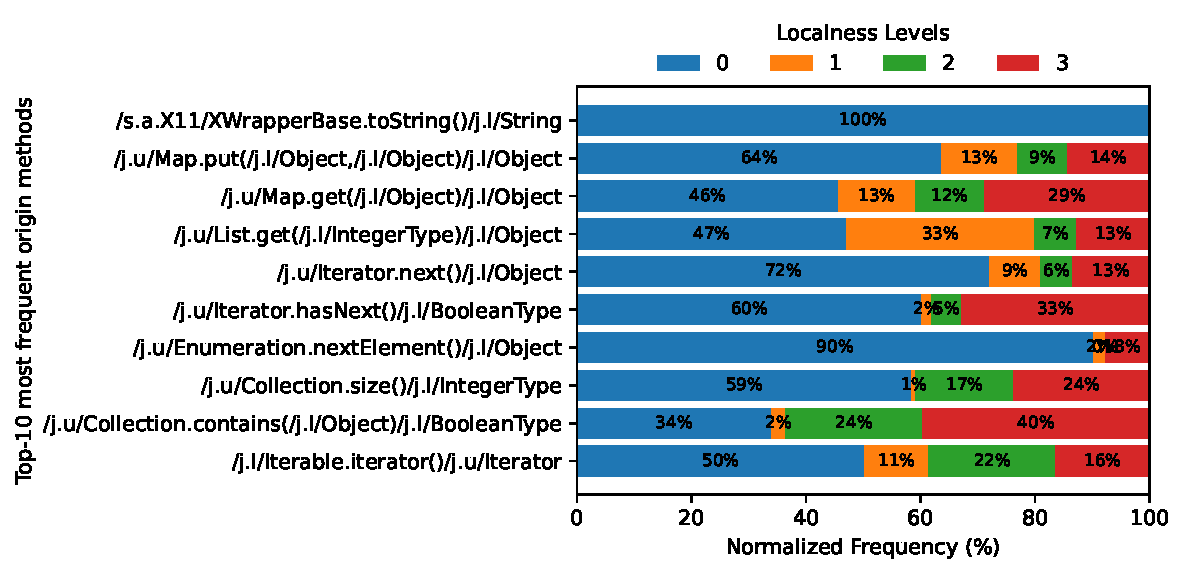
\includegraphics[width=\columnwidth]{chapters/ch2/figs/localness_normalized.pdf}
    \caption{Relative frequency of localness levels for the derivatives of the top 10 origin methods}
    \label{ch2:fig:localness}
\end{figure}

\subsection{\textbf{RQ3}: What are the effects of \tool{OriginPruner} on the size and usefulness of CGs?}
In the previous two RQs, we studied the Top-10 most common origin methods in call graphs and how local their derivatives are. Using the gained insights and findings, we prune edges in call graphs to study the effect of pruning on the size and complexity of call graphs. Also, we use the vulnerability propagation analysis as a case study to investigate the effectiveness of our proposed pruning technique for security applications where soundness is essential. In other words, if one vulnerable method is missed in the analysis due to pruning, it can be costly for developers or users by allowing attackers to exploit the vulnerable method. 

\paragraph{Methodology}
First, we prune edges call graphs by following our filtering strategy, which is an exclusion list of Top-1000 frequent origin methods. Specifically, we consider a filter of different sizes from the set $\{1,2,3,5,10,25,50,100,1000\}$ to prune edges. Basically, for each program in YCorpus, we end up with nine different pruned call graphs. Given 203 pruned CGs, we report the average and standard deviation for nodes, edges, and relative size reduction for every nine different filters, compared to the baseline, which is OPAL's static CGs. In addition, we evaluate our proposed approach in combination with an ML-based CG pruning technique, called \tool{OriginPruner} with Selective, ML-based Pruning. This approach gives edges to derivatives of the origin methods to the ML model which makes the final decision for pruning.

Second, we perform a vulnerability propagation analysis (described in Section~\ref{ch2:subsec:vpa}) for OPAL's static CG and all the pruned CGs from the previous step, given the artificial CVEs. We report the average number of vulnerable paths, reachable vulnerable nodes, and analysis time for OPAL's static cg as a baseline and every nine different filters or an exclusion list. We also repeated this experiment for  \tool{OriginPruner} with Selective, ML-based pruning. To accurately measure analysis, we consider JVM's Just-in-Time compilation by warming up the analysis program, running it three times, and reporting the average analysis time across runs. 

\paragraph{Results}
Table~\ref{ch2:tab:cg_size} shows the effect of pruning call graph size.
We compare the baseline results of an OPAL call graph with different configurations of \OP{N}, which prunes calls to all methods that are related to the Top-N origin methods, either \emph{exhaustively} or \emph{selectively} using an ML-based pruning classifier.
OPAL's static CGs are shown as a baseline at the top of the table. On average, across all programs in YCorpus, there are around 186K and 4.9M nodes and edges, respectively.
Considering exhaustive pruning, just pruning the Top-1 origin method \code{Iterator.next()} already reduces the size of call graphs from 4.9M to 4.22M on average, a reduction in size by 14\%. Notably, pruning the Top-10 origin methods reduces the CG size by 37\% to 3M edges on average.
This implies that, on average, more than one-third of edges are a call to a method that overrides one of those Top-10 most common origin methods reported in Table~\ref{ch2:tab:origin_freq}.
From Top-10 to Top-1000, we still observe a steady decrease in the size of call graphs to the point where Top-1000 reduces the number of edges by more than half on average, i.e., 58\%.

Compared to exhaustive pruning, selective pruning uses an ML-based classifier to make individual pruning decisions for each edge.
This approach also consistently reduces the size of call graphs, even though it prunes fewer edges. For instance, selectively pruning the Top-10 origin methods has almost the same effect on the CG size as exhaustive pruning of the Top-5 origin methods.
%This is sensible as the ML-based CG pruner that is based on CodeBERT uses a very conservative strategy to prune edges.
It is interesting to see that the ML-based CG pruner seems to implicitly learn the concept of origin methods from its training data: the underlying CodeBERT model is usually very conservative in its pruning decisions, yet it learns that a less aggressive pruning is required for the origin methods.

Table~\ref{ch2:tab:vuln_analysis_results} shows the effect of call graph pruning on the vulnerability propagation analysis. Starting with OPAL as a baseline, we observe that, on average, there are around 18K reachable paths and 76\% of 100 artificial CVEs are reachable from application nodes.
The artificial CVEs are randomly distributed among CG nodes, which means that they are also not necessarily reachable in the unpruned static call graphs.
When pruning the Top-1 origin methods, \tool{OriginPruner} improves the analysis time by around 19\% while preserving the same vulnerable node reachability through vulnerable paths as the unpruned CG (i.e., 76\%).
This trend continues when more is pruned.
By considering the derivatives of Top-10 most common origin methods for pruning, we observe a small 2\% decrease in the average number of reachable vulnerable nodes while the analysis time can be reduced from 72s to 49s (33\% faster).
Using \tool{OriginPruner}, it is, therefore, possible to select a trade-off between CG accuracy and size by selecting the number of origin methods to prune. Accepting a small decrease in the soundness of the vulnerability analysis can result in a significant lowering of the computational time.
We also see that there is a sweet spot.
Pruning Top-100+ origin methods substantially reduce the CG sizes, but the effects on reachability become larger with a 10+\% decrease in reachable vulnerable nodes. This makes these configurations impractical for vulnerability analysis as it can cause developers to miss the presence of vulnerabilities in their application or its dependencies.
With the selection, it is possible to obtain the same number of reachable vulnerable nodes as OPAL while using a Top-3 filter for pruning. Overall, the results of the selective approach show that the ML-based CG pruner makes our proposed approach slightly more conservative by pruning fewer edges. However, the practicality of the selective approach is still a question given its additional computational overhead.

\begin{table*}
\centering
\caption{The effect of pruning on the size of call graphs and vulnerability propagation}
\label{ch2:tab:cg_size}
\label{ch2:tab:vuln_analysis_results}
\resizebox{\columnwidth}{!}{\begin{tabular}{@{}lccccrr@{}}
\toprule
&&&& \multicolumn{2}{c}{{\bf Reachable ...}} & \\
\cmidrule{5-6}
\textbf{Approach} & \textbf{\#CG Nodes} & \textbf{\#CG Edges} & \textbf{Reduction (\%)} & {\# Paths} & {Nodes (\%)} & \textbf{Analysis Time (s)} \\
\midrule
% YCorpus
OPAL & 186k $\pm$ 27K & 4.9M $\pm$ 1.5M & 0.0 & 18.8K $\pm$ 42.8K & 0.76 $\pm$ 0.17 & 72.94 $\pm$ 25.47 \\
\midrule
\multicolumn{7}{c}{\tool{OriginPruner} with Exhaustive Pruning} \\
\midrule
\OP{1} & 186K $\pm$ 27K & 4.2M $\pm$ 1.3M &  0.14 $\pm$ 0.01 & 18.7K $\pm$ 42.3K & 0.76 $\pm$ 0.17 & 61.22 $\pm$ 18.18 \\
\OP{2} & 186K $\pm$ 27K & 3.6M $\pm$ 1.1M &  0.26 $\pm$ 0.02 & 18.6K $\pm$ 41.8K & 0.75 $\pm$ 0.17 & 57.55 $\pm$ 15.84 \\
\OP{3} & 186K $\pm$ 27K & 3.4M $\pm$ 1.0M &  0.29 $\pm$ 0.03 & 18.5K $\pm$ 41.8K & 0.75 $\pm$ 0.17 & 55.71 $\pm$ 15.83 \\
\OP{5} & 186K $\pm$ 27K & 3.3M $\pm$ 0.9M &  0.33 $\pm$ 0.04 & 18.5K $\pm$ 41.8K & 0.75 $\pm$ 0.17 & 53.49 $\pm$ 15.27 \\
\OP{10} & 186K $\pm$ 27K & 3.0M $\pm$ 0.9M &  0.37 $\pm$ 0.04 & 18.2K $\pm$ 41.6K & 0.74 $\pm$ 0.17 & 49.59 $\pm$ 12.87 \\
\OP{25} & 186K $\pm$ 27K & 2.8M $\pm$ 0.7M &  0.43 $\pm$ 0.05 & 18.1K $\pm$ 41.6K & 0.73 $\pm$ 0.16 & 47.76 $\pm$ 12.23 \\
\OP{50} & 185K $\pm$ 27K & 2.6M $\pm$ 0.7M &  0.47 $\pm$ 0.05 & 17.7K $\pm$ 40.5K & 0.72 $\pm$ 0.16 & 43.83 $\pm$ 10.41 \\
\OP{100} & 185K $\pm$ 27K & 2.4M $\pm$ 0.6M &  0.50 $\pm$ 0.05 & 15.9K $\pm$ 37.2K & 0.65 $\pm$ 0.15 & 38.82 $\pm$ 9.15 \\
\OP{1000} & 180K $\pm$ 27K & 2.0M $\pm$ 0.5M &  0.58 $\pm$ 0.05 & 13.0K $\pm$ 30.6K & 0.55 $\pm$ 0.13 & 29.76 $\pm$ 6.90 \\
\midrule \multicolumn{7}{c}{\tool{OriginPruner} with Selective, ML-based Pruning} \\ \midrule
\OP{1} & 186K $\pm$ 27K & 4.3M $\pm$ 1.4M &  0.13 $\pm$ 0.01 & 18.7K $\pm$ 42.3K & 0.76 $\pm$ 0.17 & 57.12 $\pm$ 16.67 \\
\OP{2} & 186K $\pm$ 27K & 3.7M $\pm$ 1.2M &  0.25 $\pm$ 0.01 & 18.6K $\pm$ 41,8K & 0.76 $\pm$ 0.17 & 54.53 $\pm$ 16.57 \\
\OP{3} & 186K $\pm$ 27K & 3.6M $\pm$ 1.1M &  0.27 $\pm$ 0.02 & 18.6K $\pm$ 41.8K & 0.76 $\pm$ 0.17 & 54.22 $\pm$ 15.11 \\
\OP{5} & 186K $\pm$ 27K & 3.4M $\pm$ 1.1M &  0.31 $\pm$ 0.02 & 18.6K $\pm$ 41.8K & 0.75 $\pm$ 0.17 & 51.23 $\pm$ 14.06 \\
\OP{10} & 186K $\pm$ 27K & 3.2M $\pm$ 1.1M &  0.34 $\pm$ 0.03 & 18.4K $\pm$ 41.7K & 0.75 $\pm$ 0.17 & 50.11 $\pm$ 14.12 \\
\OP{25} & 186K $\pm$ 27K & 3.0M $\pm$ 1.0M &  0.40 $\pm$ 0.03 & 18.3K $\pm$ 41.6K & 0.74 $\pm$ 0.17 & 48.35 $\pm$ 13.84 \\
\OP{50} & 185K $\pm$ 27K & 2.8M $\pm$ 0.9M &  0.44 $\pm$ 0.03 & 18.0K $\pm$ 40.6K & 0.73 $\pm$ 0.17 & 45.21 $\pm$ 12.65 \\
\OP{100} & 185K $\pm$ 27K & 2.6M $\pm$ 0.9M &  0.47 $\pm$ 0.03 & 16.5K $\pm$ 37.7K & 0.67 $\pm$ 0.16 & 41.55 $\pm$ 15.25 \\
\OP{1000} & 181K $\pm$ 27K & 2.2M $\pm$ 0.8M &  0.54 $\pm$ 0.03 & 13.9K $\pm$ 32.0K & 0.58 $\pm$ 0.14 & 33.16 $\pm$ 12.23 \\
\bottomrule
\end{tabular}}
\end{table*}

\subsection{\textbf{RQ4}: What is the computational overhead of \tool{OriginPruner}?}
The previous RQ has shown that \tool{OriginPruner} can leverage origin methods to guide the CG pruning, which can greatly reduce the size of call graphs with minimal loss in the accuracy of the analysis.
While this speeds up the graph search, these benefits must need to be computed first as call-graph pruning is a post-processing step that adds additional overhead to the call-graph generation process itself.
Therefore, we want to investigate the additional computational cost of \tool{OriginPruner} compared to basic CG generation.

\paragraph{Methodology}
First, we report the average time of call graph generation using the OPAL framework for all the programs in YCorpus. Then, we report the average pruning time of \tool{OriginPruner} for processing the Top1-1000 origin methods.
Note that we do not report the computational cost of the origin finder and localness analysis as they only need to be executed once for a dataset, similar to training an ML-based CG pruner.
Lastly, we report the average time for \tool{OriginPruner} with Selective, ML-based pruning which involves querying a CodeBERT-based model for pruning edges found by our approach.

\begin{table}
\centering
\caption{Run-time of CG generation and pruning}
\label{ch2:tab:cg_pruning_time}
\begin{threeparttable}
    \begin{tabular}{@{}lrr@{}}
\toprule
& \multicolumn{2}{c}{{\bf Pruning Time [s]}} \\
\cmidrule{2-3}
\textbf{Approach} & Exhaustive & Selective \\
\midrule
% YCorpus
Top-1 & 10.6 $\pm$ 3.1 & 726.9 $\pm$ 935.5 \\
Top-2 & 10.1 $\pm$ 3.0 & 705.1 $\pm$ 897.3 \\
Top-3 & 9.8 $\pm$ 2.9 & 694.4 $\pm$ 844.9 \\
Top-5 & 9.5 $\pm$ 2.8 & 611.4 $\pm$ 766.6 \\
Top-10 & 9.3 $\pm$ 2.7 & 545.7 $\pm$ 711.5 \\
Top-25 & 9.1 $\pm$ 2.6 & 521.8 $\pm$ 716.5 \\
Top-50 & 8.9 $\pm$ 2.6 & 481.8 $\pm$ 687.6 \\
Top-100 & 8.8 $\pm$ 2.5 & 439.2 $\pm$ 655.8 \\
Top-1000 & 8.8 $\pm$ 2.6 & 436.4 $\pm$ 639.0 \\
\bottomrule
\end{tabular}
\begin{tablenotes}
    \item \emph{Note:} All approaches require the same CG
generation (30.58s $\pm$ 5.06s) and Origin 
and localness analysis (99.96s $\pm$ 26.36s).
\end{tablenotes}
\end{threeparttable}
\end{table}

\paragraph{Results}
Table~\ref{ch2:tab:cg_pruning_time} shows the computational time of call graph generation and the computation time of \tool{OriginPruner}, both in the mutually exclusive, our proposed CG pruning approach, and the selective approach. The average time for CG generation using OPAL is around 30.5s for all programs in the dataset.
%Our CG generation program uses OPAL, which makes heavy use of CPU threads.
Also, the average time of the origin finder and localness analysis is about 100s. This is a one-time cost, meaning that it is similar to training an ML model, which needs to be done once for a dataset. We observe that exhaustive pruning only adds $\sim$9-10s ($\sim$33\%) overhead to the CG generation. For instance, to prune the Top-10 origin methods, the CPU time is around 9.2 seconds on average.
Such a small overhead can usually be justified by further time savings that a reduced CG size will introduce in other downstream analyses and a smaller memory footprint.

We also see that selective pruning is much more computationally expensive.
This is expected as the CodeBERT-based CG pruner model is queried for all the edges identified by \tool{OriginPruner}.
Even though we have provided caching mechanisms to speed up the model predictions, it becomes clear that the ML model does not scale well with relatively large CGs.

\section{Discussion}
In this section, we discuss the implications of the obtained results and directions for future research.

\paragraph{Promising Results}
Overall, our empirical results have shown that using an origin analysis to identify the locations in the call graph that are the main culprits for large CG sizes allows to better guide the pruning, so it only has marginal effects on analysis results.
It also seems feasible to make CG pruning part of the CG generation process. As shown in RQ4, CG pruning can be considered as a post-processing step, which adds a small overhead to CG generation, and it can even be configured to prune more or fewer origin methods, or disable the pruning altogether.
It also becomes clear that CG pruning can benefit from using truly semantic features over purely structural features even though it requires domain knowledge to tap this potential.
Future work should investigate whether other statically available facts, e.g., the distance of packages, or the existence of specific types in a class context, could be use to improve the exhaustive pruning heuristic.

\paragraph{Localness Levels}
In the RQ2, we have validated our intuition that most of the common origin methods are indeed very local to justify the exhaustive pruning.
However, the extracted localness level could also be used as a feature that can inform the pruning decision.
Maybe instead of just pruning all the Top-N origin methods, also the typical localness of subtypes for each of the Top-N origin methods should be taken into consideration and \tool{OriginPruner} should only prune such methods from the Top-N that have a very big fraction of level 0 methods.
Future work could further differentiate our localness levels in the pruning or could devise new levels or an alternate definition of localness that might be better suited for the task.

\paragraph{Limited ML Performance}
CLMs have achieved a big success in software engineering tasks like code generation, thanks to their billion-parameter-scale size~\cite{hou2024large}.
For the CG pruning task, however, it looks like are currently not yet able to outperform simple heuristics.
It is interesting to see that an ML approach would pick up a strategy for pruning origin methods that is similar to our heuristic solution and, therefore, results in a similar performance.
It does so at a massive computational cost though, which is a strong limitation.
We think that future work is necessary in two dimensions to make ML-based pruning relevant.
First, it does not seem to be sufficient to train models with basic structural features or plain source code, as the semantic features are hard to pick up during model training.
Future work needs to investigate better feature engineering or code representation to make it possible to leverage semantic features that usually require a static analysis for extraction.
Second, it is necessary to improve the scalability of ML-based pruners to make them feasible in practice.
The most promising direction is to avoid treating the pruning as a post-processing step and instead make it an integral part of a hybrid CG generator.
Note though that this optimization is also available for heuristic approaches, which makes it a particularly interesting direction to explore.

\section{Threats to Validity}
The empirical results of our work are subject to several potential threats to validity.
We will introduce these threats and our mitigation strategies.

\paragraph{Correctness}
%Concerning the internal threats to validity,
Our codebase is small and only has around 4K LoC (Java/Python).
The authors have reviewed the algorithms multiple times to prevent bugs.
Also, the CG generation and pruning have been integrated into the FASTEN project and have been used and tested by other users.

\paragraph{Representativeness}
Our choice of ML model could negatively affect selective pruning.
To mitigate this problem, we have re-used a fine-tuned CodeBERT model that has been shown to be effective for CG pruning before~\cite{mir2023effect}.

For vulnerability propagation analysis, we followed the methodology of the previous work and randomly injected artificial CVEs to call graph nodes to assess the effectiveness of \tool{OriginPruner}~\cite{mir2024effectiveness}.
While we have not tested the evaluation with actual CVEs, we do not see any reason to doubt the representative of the artificial CVEs.
However, future work should investigate this assumption.

\paragraph{Dataset}
We used an existing dataset of 23 Maven libraries, YCorpus.
We believe that our findings also hold in larger datasets.
Furthermore, the reported numbers for origin methods will only increase in our favor for larger projects, as more subtypes exist, which emphasizes the problem even more.

\section{Summary}
In this chapter, we presented \tool{OriginPruner}, a novel approach to call graph pruning, based on the origin methods and their locality to address the limitations in ML-based call graph pruning techniques, which are lack of generalization beyond training set and high inference cost. Our proposed approach leverages the insights from the origin methods, specifically, methods that introduce a signature in a class hierarchy and are frequently overridden, and their locality to prune unnecessary edges in call graphs efficiently. This approach significantly reduces the call graph size and complexity, making downstream analyses more practical for large-scale software projects. Based on the YCorpus dataset, our empirical findings reveal that specific origin methods, such as \code{Iterator.next()}, play a pivotal role in call graph complexity by being frequently overridden across different classes. We found that these methods and their derivatives have predominantly localness of Level 0 or 1, providing a solid basis for pruning without sacrificing the soundness required for tasks like vulnerability analysis. Moreover, the obtained results show that our proposed call graph pruning approach could reduce call graph size by up to 58\%, significantly improving analysis speed (up to 2.4x times) with no or minimal impact on the accuracy of downstream applications like vulnerability propagation analysis. Additionally, our approach was shown to be computationally more efficient than existing ML-based approaches, highlighting its practicality for real-world applications.
\chapter{On the Effect of Transitivity and Granularity on Vulnerability Propagation in the Maven Ecosystem}
\label{ch:effect_trans_gran}

\blfootnote{This chapter is based on the paper, Mir, A. M., Keshani, M., \& Proksch, S. (2023, March). On the Effect of Transitivity and Granularity on Vulnerability Propagation in the Maven Ecosystem. In 2023 IEEE International Conference on Software Analysis, Evolution and Reengineering (SANER'23) (pp. 201-211).~\cite{mir2023effect}.
}

\begin{abstract}
Reusing software libraries is a pillar of modern software engineering.
In 2022, the average Java application depends on 40 third-party libraries.
Relying on such libraries exposes a project to potential vulnerabilities and may put an application and its users at risk.
Unfortunately, research on software ecosystems has shown that the number of projects that are affected by such vulnerabilities is rising.
Previous investigations usually reason about dependencies on the dependency level, but we believe that this highly inflates the actual number of affected projects.
In this work, we study the effect of transitivity and granularity on vulnerability propagation in the Maven ecosystem.
In our research methodology, we gather a large dataset of 3M recent Maven packages.
We obtain the full transitive set of dependencies for this dataset, construct whole-program call graphs, and perform reachability analysis.
This approach allows us to identify Maven packages that are actually affected by using vulnerable dependencies. 
%
Our empirical results show that: (1) about 1/3 of packages in our dataset are identified as vulnerable if and only if all the transitive dependencies are considered. (2) less than 1\% of packages have a reachable call path to vulnerable code in their dependencies, which is far lower than that of a naive dependency-based analysis. (3) limiting the depth of the resolved dependency tree might be a useful technique to reduce computation time for expensive fine-grained (vulnerability) analysis.
We discuss the implications of our work and provide actionable insights for researchers and practitioners.
\end{abstract}

\newpage

\section{Introduction}
Software reuse is one of the best practices of modern software development~\cite{krueger1992software}.
Developers can easily access reusable libraries through the online open-source repositories of popular package management systems such as \tool{Maven}, \tool{NPM}, or \tool{PyPi}.
\tool{Snyk} reports that a prolific number of libraries is used in projects (40 for the average Java project) and that security vulnerabilities have steadily increased over the past few years in software ecosystems such as \tool{Maven} and \tool{NPM}~\cite{snyk21}.
While reusing libraries can substantially reduce development efforts, research has shown that it may pose a security threat~\cite{pham2010detection} and that many applications rely on libraries that may contain known security vulnerabilities~\cite{cadariu2015tracking}.
Lauinger et al.~\cite{lauinger2018thou} found that 37\% of websites in top Alexa domains have at least one vulnerable JavaScript library.
Once fixed, developers need to update their dependencies to use the new version, however, researchers have found that developers often keep outdated dependencies, making their applications vulnerable to attacks and exploits~\cite{kula2018developers}.
A lack of awareness regarding available updates, added integration efforts, and possible compatibility issues might represent factors that lead to this phenomenon.

Timing is crucial.
The Heartbleed vulnerability, a security bug in the OpenSSL library that was introduced in 2012, remained unnoticed until April 2014~\cite{durumeric2014matter}.
An Apache Log4j vulnerability was discovered end of 2021 that affected around 35K Java projects, which propagated to around 8\% of the complete Maven ecosystem~\cite{log4jvul}. 
These examples show that it is crucial to release fixes timely to not give attackers a chance to develop exploits.
We also need to gain a better understanding of how fast vulnerabilities are discovered, how they affect an ecosystem, and how long it takes until a fix is available.

In recent years, a number of studies have investigated the impact of security vulnerabilities and their propagation in the software ecosystems~\cite{decan2018impact,alfadel2021empirical,zimmermann2019small,liu2022demystifying}.
%They studied the number of projects affected by vulnerable dependencies/libraries, how long it takes to fix vulnerabilities, and how vulnerabilities propagate to the client/root applications.
The reasoning of these studies is limited to package-level analysis: they consider a project vulnerable if any (transitive) dependency contains a known vulnerability.
However, a package-level analysis cannot detect whether a client application actually uses the vulnerable piece of code, which can cause false results.
Recent works~\cite{zapata2018towards, nielsen2021modular} have overcome this limitation by performing fine-grained analysis of dependency relations in call graphs, which, as a result, increases the precision of vulnerability detection.
However, due to the computational cost of such analysis, these papers have only considered a limited number of projects.

In this chapter, we want to investigate both dimensions at once to understand how vulnerabilities propagate to projects in the Maven ecosystem.
There is a trade-off to be made between the extent of the ecosystem coverage and the precision of the analysis, so we will investigate the effect of two opposing forces:
\emph{transitivity} (direct vs. transitive dependencies) will substantially increase the search space, while a lower \emph{granularity} (package-level vs. method-level) has the chance to improve precision.
We will answer the following research questions for the \tool{Maven} ecosystem:

\begin{description}
\item[RQ1] How are security vulnerabilities distributed in Maven?
\item[RQ2] How does vulnerability propagation differ for package-level and method-level analyses?
\item[RQ3] How do vulnerabilities propagate to root packages?
\item[RQ4] Is it necessary to consider all transitive dependencies?
\end{description}

By answering the formulated research questions, we aim to provide new insights on the potential impact of software vulnerabilities in the Maven ecosystem.
Different from similar studies on the NPM and PyPi ecosystems \cite{alfadel2021empirical, decan2018impact, liu2022demystifying}, our research methodology for RQ2-4 is based on both \textit{coarse} and \textit{fine-grained} analysis. Specifically, from the transitivity perspective, we will investigate how vulnerabilities propagate to Maven projects by going from direct dependencies to transitive ones.
Additionally, we will investigate the difference between coarse-grained analysis (i.e., package-level) and find-grained analysis (i.e., method level) in vulnerability propagation.
To answer the above RQs, we have gathered a large dataset of 3M Maven projects and 1.3K security reports.

Our main empirical findings shows that, (1) transitivity has a substantial impact on the vulnerabilities propagation in Maven.
Of 1.1M vulnerable projects, only 31\% have known vulnerabilities in their \textit{direct} dependencies.
(2) The level of granularity is prominent when studying vulnerability propagation in the ecosystem.
Only 1.2\% of 1.1M transitively affected projects are \textit{actually} using vulnerable code in their dependencies.
(3) Among popular Maven projects, a vulnerability may impose higher security risk to other dependent projects if call-graph based analysis is considered.
(4) Limiting the maximum considered depth of transitive dependencies can be useful to reduce the cost of computationally-expensive, fine-grained analyses.
A slight decrease in the recall of an analysis can be traded off for a reduced computation time.

\smallskip
\noindent
Overall, this paper presents the following main contributions:
\begin{itemize}
\item We compile a public dataset for Maven that allows to study vulnerability propagation in Maven.% A  replication package with the dataset is publicly available on Zenodo
\footnote{https://doi.org/10.5281/zenodo.7540492}
\item We combine insights from previous works and closely investigate 1) a substantial part of the Maven ecosystem 2)~using method-level analysis.
\item We propose a differentiated view on transitivity that considers the distance of dependencies to an application. 
\end{itemize}

The rest of the chapter is organized as follows. Section \ref{ch3:sec:related-work} presents related work. Section \ref{ch3:sec:terms} defines the terminologies used across the paper. We present our approach to answer the formulated research questions in Section \ref{ch3:sec:approach}. Section \ref{ch3:sec:empirical-results} presents obtained empirical results. We discuss the implications of the obtained results in Section \ref{ch3:sec:discussion}. Possible threats to the validity of our results are explained in Section~\ref{ch3:sec:threats}. Finally, we conclude our work in Section\ref{ch3:sec:conclusion}.

\newpage

\section{Related Work}\label{ch3:sec:related-work}
% Package dependency networks / Ecosystem Analysis
\paragraph{Software Ecosystem Analysis}
Different characteristics of software ecosystems have been studied over the past decade. In 2016, Wittern et al.~\cite{wittern2016look} studied the evolution of the NPM ecosystem from two perspectives: (1) the growth and development activities (2) the popularity of packages. They found that package dependencies have increased by 57.9\% from 2011 to 2015.
Kikas et al.~\cite{kikas2017structure} proposed a network-based approach for studying the ecosystems of JavaScript, Ruby, and Rust. Their study shows that the growth of dependency networks for JavaScript and Ruby. Also, the removal of a single package can affect more than 30\% of projects in the ecosystem.
Decan et al.~\cite{decan2019empirical} conducted an empirical analysis of the similarities and differences between the evolution of seven different software ecosystems. Their finding shows that the package dependency network grows over time, both in size and number of updates. Also, a small number of packages account for most of the package updates.
Wang et al.~\cite{wang2020empirical} conducted an empirical study on the usages, updates, and risks of third-party libraries in the Java ecosystem. The study found that 60.0\% libraries have at most 2\% of their APIs called across projects.
Chowdhury et al.~\cite{chowdhury2021untriviality} conducted an empirical study to understand the triviality of trivial JavaScript packages. By considering the project and ecosystem usage, they found that removing one trivial package can affect up to 29\% of the entire NPM ecosystem.

Different from the aforementioned work, our work provides a new perspective on vulnerability propagation in Maven by considering the effect of both transitivity and granularity.

\begin{figure}
	\begin{center}
		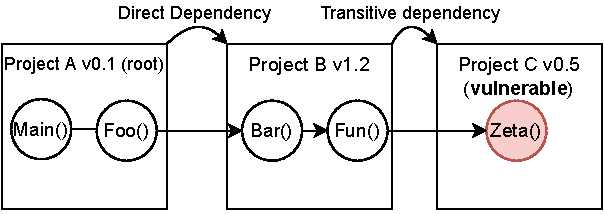
\includegraphics[width=.8\linewidth]{chapters/ch3/figs/paper-toy-example.pdf}
	\end{center} \caption{A toy example that shows a root project is transitively affected by a vulnerable dependency}
	\label{ch3:fig:toy_example}
\end{figure}


% Impact of security vulnerabilities on software ecosystems
\paragraph{Impact of vulnerabilities on software ecosystems}
In recent years, researchers have been studied the potential impact of security vulnerabilities in evolving software ecosystems. One of the earliest works is the master thesis of Hejderup~\cite{hejderup2015dependencies}. By considering 19 NPM packages, he studied how many dependent packages are infected by a vulnerability and how long it takes to release a fix after the publication of a security bug. 
Decan et al.~\cite{decan2018impact} studied the impact of security vulnerabilities on the NPM dependency network. Their study shows that approximately 15\% of vulnerabilities are considered high risk as they are fixed after their publication date.
Zimmermann et al.~\cite{zimmermann2019small} studied security threats in the NPM ecosystem. They found that a small number of JavaScript packages could impact a large portion of the NPM ecosystem. This implies that compromised maintainer accounts could be used to inject malicious code into the majority of the NPM packages.
Pashchenko et al.~\cite{pashchenko2020qualitative} performed a qualitative study to understand the role of security concerns on developers' decision-making for updating dependencies. The study found that developers update vulnerable dependencies if they are severe and the adoption of their fix does not require substantial efforts.
Inspired by the work of Decan et al.~\cite{decan2018impact}, Alfadel et al.~\cite{alfadel2021empirical} conducted an empirical analysis of security vulnerabilities in the PyPi ecosystem. Their findings show that PyPi vulnerabilities are discovered after 3 years and 50\% of vulnerabilities are patched after their public announcement.
Recently, Liu et al.~\cite{liu2022demystifying} studied vulnerability propagation and its evolution in the NPM ecosystem by building a complete dependency knowledge graph. Among their findings, they found that 30\% of package versions are affected by neglecting vulnerabilities in direct dependencies.

Considering the mentioned empirical studies on the impact of security vulnerabilities, their research methodology is based on dependency/package-level analysis, which highly over-estimates the number of packages using vulnerable dependencies. In contrast, we analyze projects in a lower granularity, i.e., call graph level in addition to the package level.

\begin{figure*}
    \centering
    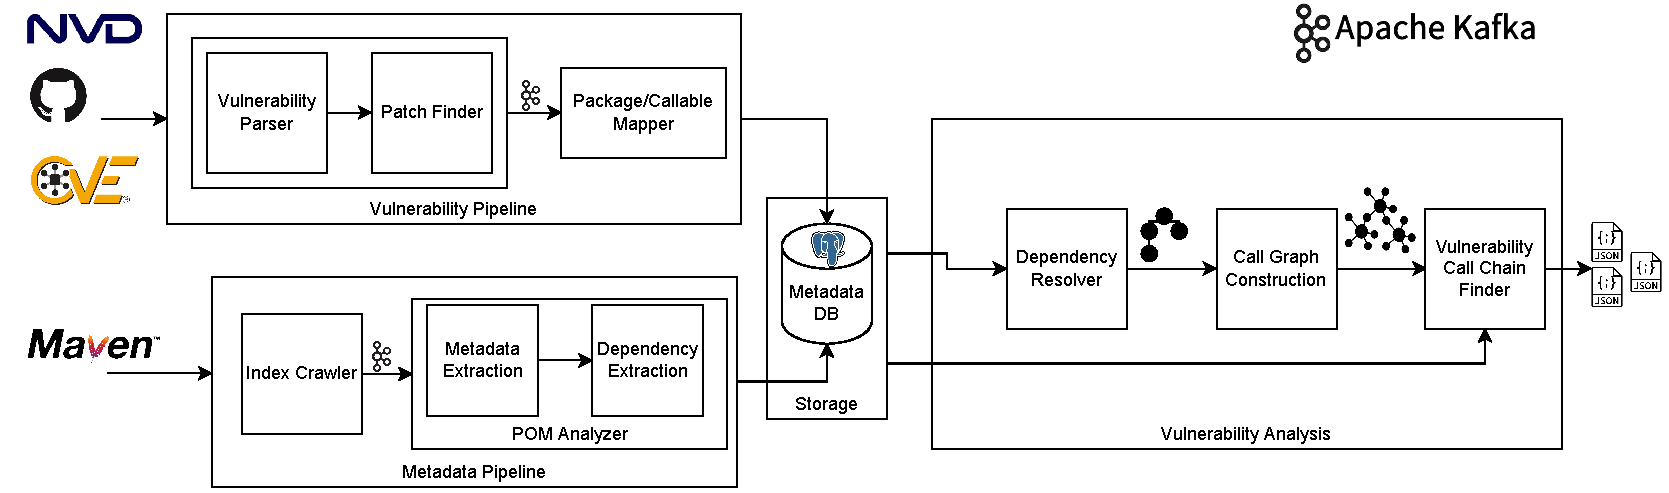
\includegraphics[width=.9\linewidth]{chapters/ch3/figs/vuln-paper-approach.pdf}
    \caption{Overview of our data processing pipeline}
    \label{ch3:fig:dp_pipeline}
\end{figure*}

\section{Terminology}\label{ch3:sec:terms}
In this section, using Figure~\ref{ch3:fig:toy_example}, we define the terminologies that we use throughout the paper.

\begin{enumerate}
\itemsep0em
    \item A \textit{project} is a reusable software component, e.g., \code{junit}. We use Maven projects/packages interchangeably in the text.
    \item A \textit{(versioned) package} is a unique release of a project, for example, \code{junit-4.12}.
    \item A \textit{dependency} is a relation to a package whose functionalities are re-used to develop new software. Dependencies can be direct or transitive, e.g., the relation \texttt{A} $\rightarrow$ \texttt{B} is direct, while the relation \texttt{A} $\rightarrow$ \texttt{C} is transitive (through \texttt{B}).
    \item A \textit{root package} is the root of the dependency tree (e.g., an application) and (transitively) depends on other packages.
    \item A \textit{vulnerability} is a defect of software that can be exploited by attackers, e.g., to gain unauthorized system access~\cite{dowd2006art}.
    \item A \textit{call graph} is a directed control-flow graph that represents the calling relationship between methods/callables in a package. For instance, in Figure \ref{ch3:fig:toy_example}, \texttt{Bar()}, defined in Package \texttt{B}, is a callable.
    \item A \textit{vulnerable call chain} is a sequence of function calls that ends in a vulnerable callable. In Figure~\ref{ch3:fig:toy_example}, the call chain \texttt{A.Main()} $\rightarrow$ \texttt{A.Foo()} $\dots \rightarrow$ \texttt{C.Zeta()} is one such example. Also, in this example, \texttt{A.Main()} $\rightarrow$ \texttt{A.Foo()} is an \emph{internal} call as both callables are defined in Package \texttt{A}, whereas \texttt{A.Foo()} $\rightarrow$ \texttt{B.Bar()} is an \emph{external} call as \texttt{B} is a dependency of \texttt{A}.
    \item A \textit{patch} is a set of code changes that fixes a vulnerability or bug in software.
    \item A \textit{patch link} is a URL or reference that points to the location where a patch can be found, typically in a version control system.
    \item A \textit{patch commit} is a specific version control commit that contains the implementation of a patch.
\end{enumerate}

\section{Approach}\label{ch3:sec:approach}
This section introduces our approach and the experimental methodology.
The overview of our data processing pipeline is shown in Figure~\ref{ch3:fig:dp_pipeline}.

\subsection{Vulnerability pipeline}
\paragraph{Vulnerability parser}
In order to create a knowledge base of vulnerability data, we gather information from various public sources (see Table~\ref{ch3:tab:vuln_sources} for details).
Each data source represents vulnerabilities in its own format and may not have complete information about a vulnerability.
Therefore, we have created a single vulnerability format that aggregates common metadata for further analysis.
The various fields of our vulnerability format are described in Table~\ref{ch3:tab:vuln_object}.
Our vulnerability knowledge base contains 1,306 security reports.% with patch information.

\begin{table}
    \centering
    \caption{List of sources for gathering vulnerability data}
    \label{ch3:tab:vuln_sources}
  \begin{tabular}{@{}lll@{}} 
				\toprule
				\textbf{Source} & \textbf{License} & \textbf{Updates} \\
    \midrule
				 National Vuln. Database (NVD)  & Public Domain  & 2 hours  \\
				GitHub Advisories  & Public Domain  & Daily  \\
				project-kb (by SAP)  & Apache License 2.0  & n/a  \\
				oss-fuzz-vulns (by Google) & CC-BY-4.0 & Daily \\
				% \hline
				% victims-cve-db  & CC BY-SA 4.0  & n/a  \\
				% \hline
				% cvedb (by fabric8-analytics)  & n/a  & n/a  \\
				\bottomrule
		\end{tabular}
%
\end{table}

\begin{table}
    \centering
    \caption{Description of our common vulnerability format}
	\label{ch3:tab:vuln_object}
 	\begin{tabular}{@{}lp{10cm}@{}} 
				\toprule
				\textbf{JSON Field} & \textbf{Description}  \\
				\midrule
				ID  & A unique id (E.g. CVE-2018-9159)   \\
				Purls & Universal URLs that represent vulnerable packages~\cite{purl} \\
				CPE & A structured naming scheme that represents information technology systems, software, and packages~\cite{cpe}  \\
				CVSS score & A numeric value for showing the severity of software vulnerabilities from 0.0 to 10.0~\cite{cvss} \\
				CWE &  A list of software weakness types~\cite{cwe} \\
				Severity level &  Qualitative severity rating scale based on CVSS scores~\cite{cvss} \\
				Published date & The date that a vulnerability is publicly announced \\
				Last modified date & The date that a vulnerability's metadata is updated \\
				Description &  An English description of  what software systems are affected by a vulnerability \\
				References & Extra web links that provide more information about a vulnerability \\
				Patch & Links to patch information and commits \\
				Exploits & Links to how to exploit a vulnerability \\
    \bottomrule
		\end{tabular}
\end{table}

\paragraph{Patch finder}
Patch information is not always available in the references of vulnerabilities by security advisories.
Therefore, it requires manual effort to tag a reference as a patch link. Also, to find vulnerable callables/methods, we do need patch commits that show modified methods after fixing a vulnerability.

We have devised a patch-finding procedure to automate the gathering of patch commits by analyzing vulnerability references. 
%The logic of the devised procedure is shown in Figure \ref{fig:patch_finder}. 
We perform the following steps to find patch commits from references.
%, one of the below steps depending on the type of the given reference:

\begin{itemize}
	\item For GitHub, GitLab or BitBucket references, if a reference points to a commit, we directly parse the commit. In the case of pull requests, we look for the merging commit and parse it. For issues, we look for linked pull requests or commits that mention them.
	\item In references to issue trackers (Bugzilla and Jira), we look for attachments or references in the comments of an issue.
	\item If a reference points directly to a Git commit, SVN or Mercurial revisions, we parse the linked code.
\end{itemize}

After parsing a patch commit, we compute the diff of modified files in the commit. Then we create pairs of filenames and their modified line numbers. This enables us to locate modified callables in the patch commit.

\subsection{Package/callable mapper}
\paragraph{Determine vulnerable package versions}\label{subsec:det-pkg-vuln}
Considering the package-level analysis of vulnerabilities, we first identify the releases of a project that is affected by a vulnerability.
To do so, we extract and analyze vulnerability constraints in security reports.
Of all the considered vulnerability sources in Table~\ref{ch3:tab:vuln_sources}, we only use the GitHub Advisory database\footnote{https://github.com/github/advisory-database} to extract vulnerability constraints as these get reviewed by an internal security team before publication.

To explain the analysis of vulnerability constraints, consider the vulnerability constraint \texttt{$>$1.0,$<$2.0} which shows that every version between 1.0 and 2.0 is vulnerable. To compute affected releases of a project, we perform a similar approach to the previous studies~\cite{decan2018impact}, which is described as follows.
Let us denote a project and its versions/releases by $P$ and the set $V$, respectively. To find the vulnerable versions of $P$, denoted by $V_{n}$, affected by the vulnerability $V$, The package mapper (See Figure \ref{ch3:fig:dp_pipeline}) automatically performs the following steps:
\begin{enumerate}
    \item Compute the set $V$ by scraping available releases on Maven Central at the time of the request.
    \item To obtain the set $V_{n}$:
    \begin{enumerate}[noitemsep]
        \item Analyze every vulnerability constraint defined in $V$ and find affected versions if they exist in $V$,
        \item Add all affected versions to $V_{n}$, i.e., $V_{n} \subset V$.
    \end{enumerate}
\end{enumerate}
 
 To obtain dependents that are affected by the vulnerable project $P$, we simply check if dependents rely on one of the affected versions in $V_{n}$.

 \paragraph{Determine vulnerable callables}
Given a vulnerability with patch information and an affected versioned packages, to identify vulnerable callables, the callable mapper automatically annotates the nodes of its call graphs with vulnerability data as follows:
\begin{enumerate}
\itemsep0em
\item Identify the last vulnerable version $P_{lv}$ and the first patched version $P_{fp}$.
\item For both $P_{lv}$ and $P_{fp}$, find files that are modified in the patch commit.
\item Locate callables whose start and end lines include the modified lines in the patched file(s) in $P_{fp}$.
\item For located callables, propagate the vulnerability to all the affected versions for which we can find the same callables. 
\end{enumerate}

\subsection{Metadata pipeline}
\paragraph{Maven index crawler}\label{ch3:subsec:dataset}
For our study, we gather versioned packages from Maven Central, which is one of the most popular and widely used repositories of Java artifacts.
We consider packages that were released between Sep. 2021 and Sep. 2022.
The resulting dataset consists of about 3M unique versioned packages of about 200K projects.
In Maven, versioned packages are differentiated by a unique Maven coordinate that consists of ids for group, artifact, and version (i.e., \texttt{g:a:1.2.3}).

\paragraph{POM Analyzer}
Maven projects are described in a central configuration file, the \code{pom.xml}~\cite{mvnpom}.
We parse these files using the same utils that are built into Maven and extract metadata information such as release date, Maven coordinate, repository/sources URL, and the list of dependencies defined in the POM file.
%These information are then stored in the metadata database, which is described in subsection \ref{subsec:storage}.

\subsection{Storage}\label{ch3:subsec:storage}
The results of both vulnerability and metadata pipelines are stored in a relational SQL database. The database schema has two SQL tables for storing metadata and dependencies of versioned packages. For storing vulnerability data, there is a SQL table to store vulnerability IDs and their corresponding statement in a JSON field. Due to the space constraint, readers can refer to our replication package for more information on the database schema.

\subsection{Analyzer pipeline}
\paragraph{Dependency resolution}\label{ch3:subsec:dep-res}
To assess how a vulnerability in a Maven package affects other projects, it is necessary to reconstruct the dependency set of a versioned package.
We resolve all versioned packages that are included in our dataset using \tool{Shrinkwrap},%
\footnote{https://github.com/shrinkwrap/resolver}
a \tool{Java} library for \tool{Maven} operations.
This downloads both the \code{pom.xml} files and the .jar files of all relevant packages into the local \code{.m2} folder.
\tool{Shrinkwrap} can resolve a complete dependency set for a given coordinate.
By statically analyzing the pom files, we can reconstruct dependency trees from this dependency set, which allows us to limit the resolution and, for example, to only include dependencies up to a certain depth.

\paragraph{Call-graph construction}\label{ch3:subsec:cg-gen}
To study the effect of granularity on vulnerability propagation we perform callable-level analysis on call graphs.
We generate whole-program static call graphs for a given Maven package using \tool{OPAL}~\cite{eichberg2014software, reif2016call, opalp}, a state-of-the-art static analysis framework for Java programs.
We configure \tool{OPAL} to use a \emph{Class Hierarchy Analysis}~(CHA) for the call graph construction~\cite{grove1997call, reif2016call}, which scales well for performing a large-scale study.
We also configured \tool{OPAL} to run with an \emph{open-package assumption}~(OPA), which will treat all non-private methods as entrypoints for the analysis.
This makes conservative worst-case assumptions and produces sound call graphs~\cite{reif2016call}, which is useful for security analysis such as our vulnerable call chain analysis.

\paragraph{Identification of vulnerable call chains}
To determine whether any method of a versioned package calls vulnerable code from one of its transitive dependencies, we need to find at least one reachable path from the method to another vulnerable method. To achieve this, we perform a Breadth-First Search (BFS) on the whole-program call graph of the versioned package plus its transitive dependencies. While traversing the graph, we compute the shortest path from the versioned package's nodes to the vulnerable node(s). Finally, we end up with a list of vulnerable call chains and their corresponding vulnerabilities.

\subsection{Implementation details \& experimental setup}
Our whole data processing pipeline (Figure \ref{ch3:fig:dp_pipeline}) is written in Java.
The pipeline has extensible components that communicate with each other either via Apache Kafka messages or through a Postgres database.
%To interact with the database, we employed the JOOQ library.
We used JGraphT for graph traversal and operations, which provides fast and memory-efficient data structures.
We ran our experiments on a Linux server (Ubuntu 18.04) with two AMD EPYC 64-Core CPUs and 512 GB of RAM. We used Docker and Kubernetes to have multiple instances of our vulnerability analyzer application to perform fine-grained analysis at a large scale. Using the above Linux machine, it took about 2 months to analyze the whole dataset with 3M versioned Maven packages.

\newpage
\section{Empirical Results}\label{ch3:sec:empirical-results}
In this section, we present the results of our empirical study. For each RQ, we describe a motivation, the methodology used to answer the research question, and discuss the obtained results of our analysis.

% TODO: Summarize the findings of the RQ1
\subsection{\textbf{RQ1}: How are security vulnerabilities distributed in the Maven ecosystem?}

%\paragraph{Motivation}
Previous work has shown a steady increase of projects/packages in the NPM and PyPi ecosystems~\cite{decan2018impact,alfadel2021empirical}. At the same time, security vulnerabilities have become more prevalent over the past decade. As expected, an increase in the infection of projects by vulnerabilities was observed~\cite{alfadel2021empirical}. This also creates an opportunity for attackers to craft exploits. Hence, in this RQ, we are motivated to study the distribution of security vulnerabilities in our dataset from three angles: (1) the evolution of discovered vulnerabilities over time (2) how many versioned packages are affected by vulnerabilities; and (3) what are the most commonly identified types of vulnerabilities in Maven.

The results of RQ1 do not present an extensive analysis of Maven vulnerabilities.
Instead, we follow the example of previous empirical studies~\cite{decan2018impact,alfadel2021empirical} and present useful statistics from our vulnerability dataset that can inform future research.

\paragraph{Methodology}
To answer the RQ1, we follow the methodology of Alfadel et al.~\cite{alfadel2021empirical} by performing three analyses as follows. In the first analysis, we group the discovered security vulnerabilities for the Maven projects by the time they were reported. Then, we show how vulnerabilities and affected Maven projects evolve per year. Additionally, we group newly discovered vulnerabilities per severity level. This helps to quantify the threat levels in the ecosystem.

In the second analysis, given that a vulnerability can potentially affect many versioned packages, we show how vulnerable Maven versioned packages are distributed. To do so, we consider the version constraint in our dataset to identify the list of affected versions by a vulnerability.

In the third analysis, we group the most commonly identified vulnerability types in the Maven ecosystem. In our dataset, each vulnerability is associated with a \emph{Common Weakness Enumeration} (CWE), a category of software weaknesses. Finally, we count the frequency of vulnerability types to show the most common vulnerabilities in the Maven ecosystem. Similar to the first analysis, we break the analysis by severity levels to show the distribution of threat levels for each vulnerability type. 

\paragraph{Findings}
From Figure \ref{ch3:fig:vuln_affected_pkgs}, it can be seen that both vulnerabilities and affected projects have steadily increased in the Maven ecosystem. For instance, in 2014, 15 Maven projects were affected by vulnerabilities. In 2018, 223 Maven projects were affected, an increase of almost 15 times.

Figure \ref{ch3:fig:vuln_sev} shows the vulnerability introduction by severity level. Overall, we observe that vulnerabilities with critical and high severity levels have increased significantly over the past couple of years. Considering vulnerabilities with high severity, in 2017, 64 vulnerabilities were discovered, this number doubled in 2021, i.e., 128 vulnerabilities. This suggests that attackers may have a higher chance to craft an exploit and damage the affected software systems.

From Figure \ref{ch3:fig:dist_no_vers}, it can be observed that Maven projects release often with a median of 81 unique versions.
The median Maven project also has 26 vulnerable versions, which shows that 32\% of all projects are affected considering available versions at the time of vulnerability discovery.

Our dataset contains 114 distinct software weaknesses (CWEs). Table \ref{ch3:tab:vuln_cwe_dist} shows the top 5 common software weaknesses in the Maven projects. Overall, these 5 software weaknesses account for 37\% of all the discovered vulnerabilities.
The most common vulnerability type is the \emph{deserialization of untrusted data} (CWE-502), most of which are of critical or high severity levels. This indicates a major threat to the affected Maven projects by CWE-502.

\begin{figure}
    \centering
    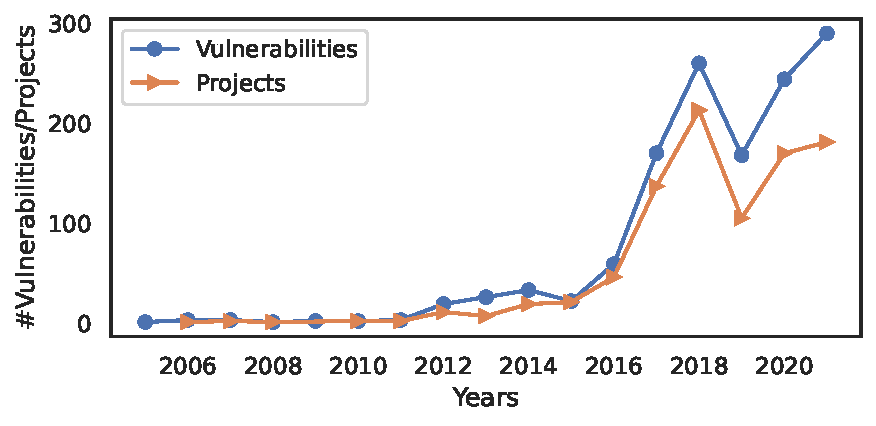
\includegraphics[width=1\linewidth]{chapters/ch3/figs/vuln_affected_pkg.pdf}
    \vspace{-18pt}
    \caption{Vulnerability Introduction Into Maven by Year}
    \label{ch3:fig:vuln_affected_pkgs}
%
    \vspace{9pt}
%
    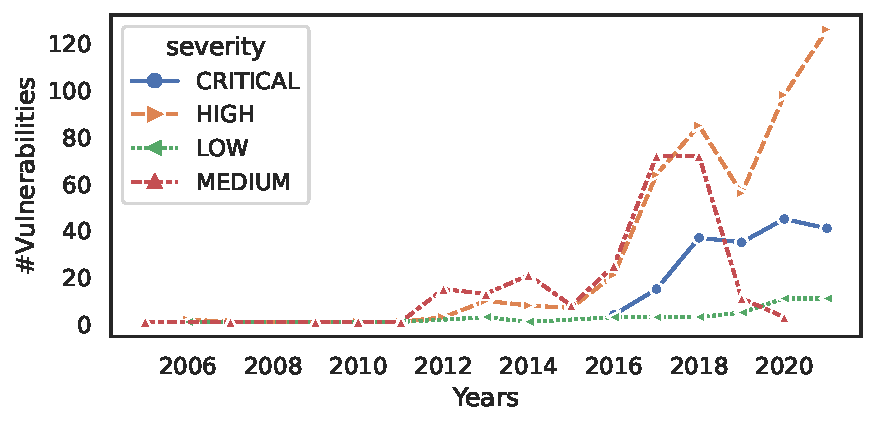
\includegraphics[width=1\linewidth]{chapters/ch3/figs/vuln_severity.pdf}
    \vspace{-18pt}
    \caption{Vulnerability Introduction by Year and Severity}
    \label{ch3:fig:vuln_sev}
% %
%     \vspace{9pt}
% %
\end{figure}
\begin{figure}
	\begin{subfigure}{0.31\columnwidth}
			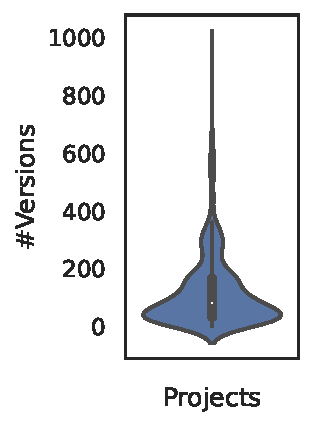
\includegraphics[width=\textwidth]{chapters/ch3/figs/no_pkg_vers.pdf}
		    \caption{Total Projects}
		    \label{ch3:fig:dist_no_vers}
	\end{subfigure}
\hfill
\begin{subfigure}{0.31\columnwidth}
	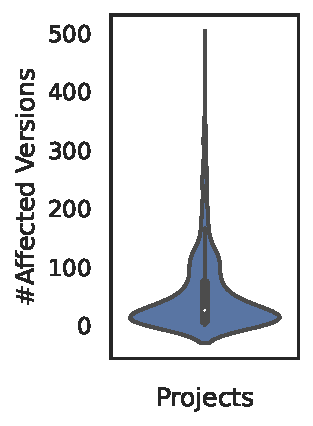
\includegraphics[width=\textwidth]{chapters/ch3/figs/no_affected_vers.pdf}
    \caption{Vulnerable}
    \label{ch3:fig:dist_no_affected_vers}
\end{subfigure}
\hfill
\begin{subfigure}{0.31\columnwidth}
	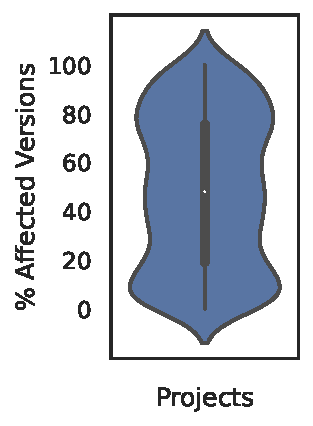
\includegraphics[width=\textwidth]{chapters/ch3/figs/no_affected_vers_in_pkgs.pdf}
	\caption{Vulnerable (\%)}
	\label{ch3:fig:dist_per_affec_vers}
\end{subfigure}
\caption{Vulnerability distribution among projects in the dataset}
\label{fig:dist_vuln_pkgs}
\end{figure}

\begin{table*}
    \centering
    \caption{Top 5 most commonly found vulnerability types in Maven}
    \label{ch3:tab:vuln_cwe_dist}
    \resizebox{\columnwidth}{!}{\begin{tabular}{@{}lrrrrrr@{}}
    \toprule
        && \multicolumn{5}{c}{{\bf Frequency by Severity}} \\
        \cmidrule{3-7}
    {\bf Vulnerability type (CWE)} & {\bf Freq.} &  Critical & High & Moderate & Medium & Low \\
    \midrule
    Deserialization of Untrusted Data (CWE-502) & 166 & 52 &85 &17& 12 & 0 \\
    Cross-site Scripting (CWE-79) & 108 & 0 & 2 &72 & 27 & 7 \\
    Improper Input Validation (CWE-20) & 88 & 6 & 47 & 15 & 20 & 0 \\
    Improper Restriction of XML External Entity Reference (CWE-611)& 78 & 21 &32 & 10 & 11 & 4 \\
    Path Traversal (CWE-22) & 65 & 4 & 24 &18 & 19 & 0 \\
    \midrule
    Total & 505 & 83 & 190 & 132 & 89 & 11 \\
    \bottomrule
\end{tabular}}
\end{table*}

\paragraph{Comparison to the NPM and PyPi ecosystems} Similar to the existing studies on these two ecosystems~\cite{alfadel2021empirical,decan2018impact}, we also observe that security vulnerabilities have increased over time. However, Maven packages have substantially more releases, on median, 81 releases whereas PyPi, on the median, has 29 releases. Also, as expected, Maven packages have more vulnerable versions, i.e., 26, on the median, compared to 18, on the median, in PyPi.

\subsection{\textbf{RQ2}: How do vulnerabilities propagate to Maven projects considering dependency- and callable-level analyses?}

%\paragraph{Motivation}
In the RQ2, we are interested in studying the effect of \textit{transitivity} and \textit{granularity} on the propagation of security vulnerabilities to Maven projects. This is different from prior similar studies~\cite{zimmermann2019small, liu2022demystifying}, which considered a project as vulnerable if one of its dependencies contain a vulnerability. This overestimates the number of affected projects and hence it may introduce false positives. Moreover, as shown in a recent study~\cite{ponta2020detection}, a project is not affected if it does not call vulnerable code in its dependencies. Specifically, from the transitivity perspective, we want to find out how many versioned packages are \textit{potentially} affected by a known vulnerability in their direct or transitive dependencies. From the granularity perspective, we want to know how many versioned packages are \textit{actually} affected by calling vulnerable code.

\paragraph{Methodology}
To answer RQ2, we perform our experiment on our Maven dataset using four distinct analysis settings:

\begin{description}
%
\item[$D_p(max)$:]  A package-level analysis that includes all transitive dependencies.
%It computes how many versioned Maven projects are  \textit{transitively} affected by using vulnerable dependencies, considering the whole dependency tree.
%    To do this, first, we need to obtain the transitive dependency set of all the versioned packages of our dataset, which is described in subsection \ref{subsec:dep-res}.
%
\item[$D_p(1)$:]
A package-level analysis on only direct dependencies.
%It is similar to $D_p(max)$, but only considers the set of all directly dependencies.
%
\item[$D_m(max)$:]
A callable-level analysis that includes all transitive dependencies.
It computes how many versioned packages are \textit{actually} affected by calling vulnerable code from their transitive dependencies.
In the whole-program call graph that we create using the OPAL framework, we mark nodes as vulnerable if modified functions in the patch commit match the signature of the node.
If there is at least a path from a node of the root project to a vulnerable node in its transitive dependencies, we consider the versioned project affected by a vulnerability.
%
\item[$D_m(1)$:]
A callable-level analysis that is similar to $D_m(max)$, but which only considers direct dependencies.
%The methodology  with the exception that we only consider direct dependencies when building a whole-program call graph and performing reachability analysis. 
%
\end{description}

The subsequent sections will refer to these four defined settings.

\paragraph{Findings}
Figure~\ref{ch3:fig:vuln_affected_pkgs} shows the number of affected versioned packages considering the four described analyses in the methodology of the RQ2. Notice that the x-axis is scaled using $log_{10}$. Considering the $D_p(max)$ analysis, we observe that about $10^{6}$ versioned packages are affected by a known vulnerability in their transitive dependency set. This amounts to 40\% of versioned packages in our dataset, affected by 517 CVEs. Considering the $D_p(1)$ analysis, however, only 369K package versions are affected by using vulnerable direct dependencies, which is significantly lower than that of the $D_p(max)$ setting. This is expected as the full transitive dependency set is larger than a direct dependency set.

From Figure ~\ref{ch3:fig:vuln_pkgs_analysis_comparison}, we also observe that the callable level analysis, $D_{m}$, detects much lower vulnerable versioned packages compared to the package level analysis, $D_{p}$, i.e., $10^{4.15} \ll 10^{6}$. This is because, for the $D_{m}$ setting, we perform reachability analysis to determine whether the vulnerable method in (transitive) dependencies is used whereas the $D_{p}$ setting is naive as it only checks the presence of a known vulnerability in the (transitive) dependency set. Another intriguing observation is that the set $|D_{m}(1)|=10^{3.88}$ contains more than half of the vulnerable versioned packages in the set $|D_{m}(max)|=10^{4.15}$, i.e., $|D_{m}(1) \cap D_{m}(m)|/|D_m(m)|=0.53$.

\begin{figure}[!t]
    \centering
    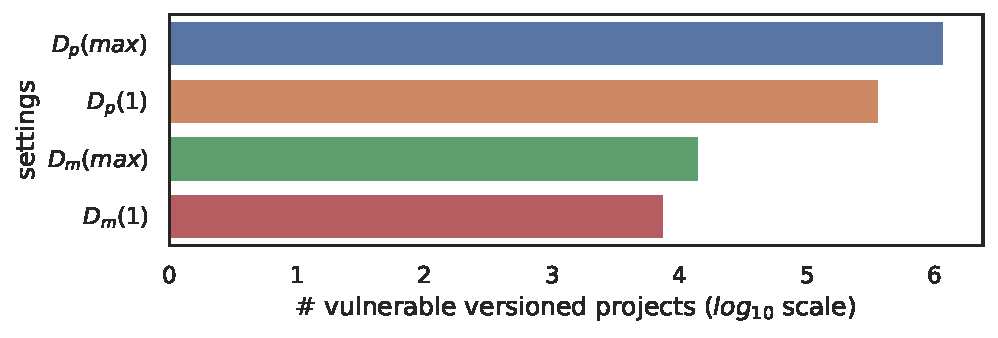
\includegraphics[width=\columnwidth]{chapters/ch3/figs/vuln_pkg_ver_dp_vs_dm.pdf}
    \caption{Number of vulnerable packages with different analysis settings}
    \label{ch3:fig:vuln_pkgs_analysis_comparison}
\end{figure}
% %
% \vspace{\distPlot}
% %

\subsection{\textbf{RQ3}: How does the propagation of security vulnerabilities affect root packages?}

%\paragraph{Motivation}
A security vulnerability in a popular package can propagate to affect many other packages in the package dependency network. This is also confirmed by a recent study~\cite{zimmermann2019small}, showing that a small number of JavaScript packages can affect a large portion of the NPM ecosystem. Therefore, we want to study how the propagation of security vulnerabilities can affect a large portion of packages and versioned packages in the Maven ecosystem. We analyze this research question from two perspectives: (1) how vulnerabilities propagate to root packages by considering transitive dependencies and (2) how vulnerabilities propagate to root packages by considering the usage of vulnerable code in dependencies.

\paragraph{Methodology}
We combine two different strategies to investigate how vulnerabilities propagate to root packages.
First, at the package level, we iterate through the full transitive dependency set of versioned packages, which is already obtained from the RQ2, i.e., the $D_{p}(max)$ setting.
We check if at least one element in the dependency set has a known vulnerability, if yes, we consider the root versioned package as vulnerable.
We list the top 10 frequent vulnerabilities that exist in the dependency trees of all the versioned projects in our dataset.
This approach overestimates the number of affected root packages, but it follows previous work~\cite{liu2022demystifying}.

Second, to analyze vulnerability propagation through vulnerable callables, we use the whole-program call graphs of versioned packages and their transitive dependencies from RQ2, i.e., $D_{m}(max)$, and then we extract known vulnerabilities, CVEs, and their corresponding vulnerable call chains.
Given these, we obtain the number of versioned packages that are actually affected by the top 10 frequent CVEs.

\begin{table*}
    \centering
    \caption{Top-10 CVEs that potentially/actually affect most package versions}
    \label{ch3:tab:top10-cves}
    \begin{threeparttable}
    \resizebox{\columnwidth}{!}{\begin{tabular}{@{}llrrcrr@{}}
\toprule
   & & \multicolumn{2}{c}{{\bf Number of Packages}} && \multicolumn{2}{c}{\bf \%Proportion\tnote{1}} \\
    \cmidrule{3-4}
    \cmidrule{6-7}
    {\bf CVE ID} &                              {\bf Project} & Potentially Affected & Actually affected && $D\_p(max)$ & $D\_m(max)$ \\
\midrule
  CVE-2020-36518 & com.fasterxml.jackson.core:jackson-databind &                                  233,430 &                               1,153 &&                     19.6 &                      8.1 \\
  CVE-2022-24823 &                   io.netty:netty-codec-http &                                  142,177 &                                  90 &&                     11.9 &                      0.6 \\
  CVE-2022-24329 &          org.jetbrains.kotlin:kotlin-stdlib &                                   82,060 &                                  32 &&                      6.9 &                      0.2 \\
  CVE-2021-37137 &                        io.netty:netty-codec &                                   57,535 &                                 525 &&                      4.8 &                      3.7 \\
  CVE-2021-22569 &         com.google.protobuf:protobuf-kotlin &                                   57,095 &                                 390 &&                      4.8 &                      2.7 \\
CVE-2018-1000632 &                                 dom4j:dom4j &                                   47,820 &                               1,438 &&                      4.0 &                     10.1 \\
  CVE-2022-25647 &                   com.google.code.gson:gson &                                   47,372 &                                 171 &&                      4.0 &                      1.2 \\
   CVE-2020-8908 &                      com.google.guava:guava &                                   42,084 &                                  84 &&                      3.5 &                      0.6 \\
  CVE-2022-22965 &          org.springframework:spring-webflux &                                   38,882 &                                 572 &&                      3.3 &                      4.0 \\
  CVE-2018-20200 &                  com.squareup.okhttp:okhttp &                                   38,466 &                                  30 &&                      3.2 &                      0.2 \\
\bottomrule
\end{tabular}}

    \begin{tablenotes}
    \item[1] {\footnotesize
    The percentage of affected packages in the set $D_{p/m}(max)$. \\ See the methodology of the RQ2 for the definition of $D_{p/m}(max)$.}
  \end{tablenotes}
\end{threeparttable}
\end{table*}

\paragraph{Findings}
Table \ref{ch3:tab:top10-cves} shows the top-10 CVEs that affect most versioned packages in the Maven dataset considering both dependency- and callable-level analysis.
It can be observed that the two Maven projects \texttt{jackson-databind} and \texttt{netty-codec-http} potentially affect 375,607 versioned packages in the Maven ecosystem, which is substantially higher than any other CVEs reported in Table \ref{ch3:tab:top10-cves}.
Also, even considering just the top-10 CVEs, together they already affect 786,921 versioned Maven projects, which accounts for 66.1\% of all the identified vulnerable versioned packages in the whole dataset (see $D_p(max)$ in Figure \ref{ch3:fig:vuln_pkgs_analysis_comparison}).

The results of the callable-level analysis paint a different picture.
Only 4,485 versioned Maven packages are actually affected by the top-10 CVEs.
This clearly illustrates that vulnerability analyses that only consider the package level result in a significant overestimation of vulnerable packages in the Maven ecosystem.
A second important observation is that any threat estimation will come to different conclusions, depending on whether a package-level or a callable-level granularity is being considered.
For instance, \texttt{CVE-2022-24823} (second row), accounts for 11.9\% of all potential affections, but only for 0.6\% actually affected elements.
On the other hand, \texttt{CVE-2018-1000632} (sixth row) looks much less problematic on first glance, being responsible for only 4\% of the potential affections.
However, the number of actual affections that we found is even higher than the top-1 vulnerability in the list.
This suggests that $D_p(max)$ and $D_m(max)$ do not necessarily correlate with each other when studying the vulnerability propagation and its impact on other projects.

\subsection{\textbf{RQ4}: Is considering all transitive dependencies necessary?}
The ${D_{m}(max)}$ setting can be deemed as the "best" approach to achieve high recall and precision in the vulnerability analysis. However,
to perform such analysis, one needs to compute a whole-program call graph of a versioned package plus its full transitive dependency set. This can be a very expensive task if done at the ecosystem level, i.e., a large-scale study with millions of versioned packages.
This research question investigates if it is possible to "cut-off" dependencies that are distant in the dependency tree.
Such pruning will reduce the size of the dependency set and has a chance to speed up the fine-grained analysis at the cost of a decrease in the recall of the analysis.
We want to analyze this tradeoff.

\paragraph{Methodology}
We perform two analyses. First, we construct whole-program call graphs for all the elements of $D_{m}(max)$ and perform a reachability analysis at the dependency levels 1 to 5. This analysis produces five sets, i.e., $D_{m}(1), \dots, D_{m}(5)$. All of them are a subset of $D_{m}(max)$ (e.g., $D_{m}(2) \subset D_{m}(max)$).
%
In the second analysis, we find the maximum dependency depth for each versioned package in $D_m(max)$.
With this information, we iterate over the elements of $D_{m}(max)$ and count the number of reachable vulnerabilities at each dependency level until the maximum level is reached. We repeat this process for the other sets.%, i.e., $D_{m}(1), \dots, D_{m}(max)(5)$.

\begin{figure}
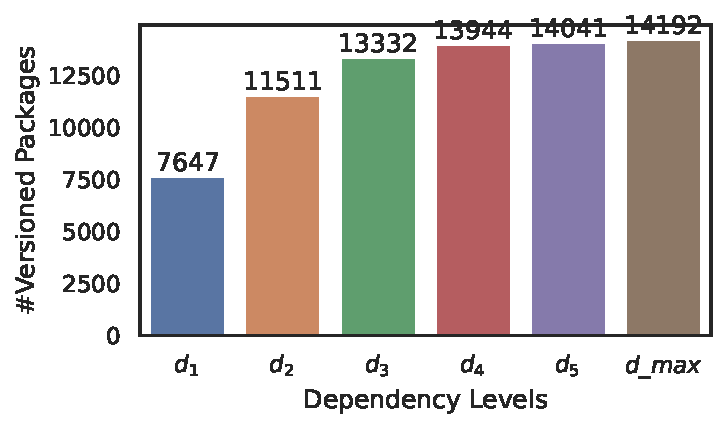
\includegraphics[width=0.8\columnwidth]{chapters/ch3/figs/pkg_num_dep_level.pdf}
    \caption{Number of vulnerable packages on various dependency depths}
    \label{ch3:fig:num_vuln_pkg_d_levels}
\end{figure}

\paragraph{Findings}
Figure~\ref{ch3:fig:num_vuln_pkg_d_levels} shows the number of vulnerable versioned packages while performing callable-level analysis and considering different dependency levels. Using only direct dependencies, i.e., $D_{m}(1)$, 55.8\% of vulnerable versioned packages are detected comparing to $D_m(max)$. This observation is in line with the findings of RQ2 (see Figure~\ref{ch3:fig:vuln_affected_pkgs}).
Every additional layer can identify more vulnerable packages, but dependency level 3 already reaches 94\% coverage.
Cutting off at this level will result in an analysis that will miss some vulnerabilities.
While this might not be acceptable for security-sensitive analyses, other analyses could leverage this finding to potentially save substantial computation time.

\begin{figure}
    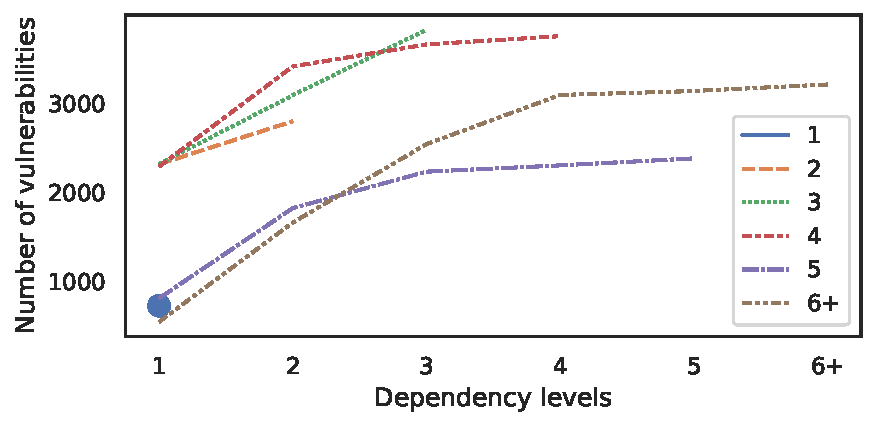
\includegraphics[width=0.8\linewidth]{chapters/ch3/figs/num_vuln_dep_levels.pdf}
    \caption{Number of vulnerabilities on various dependency depths}
    \label{ch3:fig:num_vuln_dep_levels}
\end{figure}

Figure~\ref{ch3:fig:num_vuln_dep_levels} investigates these results with a different visualization.
The different plot lines represent packages with vulnerabilities on the exact dependency level $1,2,..., 6+$.
The y-axis shows how many of the existing vulnerabilities can be found when the dependency tree is cut of at depth $d$.
As expected, vulnerable versioned packages with transitive dependencies tend to be affected by more vulnerabilities than versioned packages with only direct dependencies.
However, we see a common pattern across the different plots: the increase slows and starts to converge at dependency level 3-4.
Programs that have such deep dependency levels also have large dependency set, so for these projects, the potential saving in the analysis effort seems to be particularly beneficial.

To estimate how much computation time can potentially be reduced, we approximate the required computation time with the size of the transitive dependency set.
This is likely a lower bound, as the number of call-graph edges grows much faster than linearly.
Figure~\ref{ch3:fig:num_deps_levels} shows the distribution over the dependency set sizes for all packages in $D_m(max)$, which have a dependency tree with the exact height.
For example, the first box plot in the diagram contains all versioned packages that only have direct dependencies.
The average size of their dependency set is close to 0, whereas packages with 3 dependency levels have a median of 24 dependencies, and 6+ dependency levels even go up to a median of 147 dependencies.
Even if we only assume a linear growth in computation time, filtering the large applications to dependency level 3 would lead to an enormous analysis speed-up of about 6 times.
These large applications are usually also the limiting factor when it comes to computation timeouts or memory consumption of analyses.
    
\section{Discussion}\label{ch3:sec:discussion}
In this section, we discuss actionable results and provide insights from our study.

\paragraph{Granularity Matters}
When studying security vulnerabilities, granularity matters.
As shown in RQ2 and RQ3, dependency-level analysis highly overestimates the number of vulnerable packages in the Maven ecosystem.
A project is not affected if the vulnerable code/callable is never reached. This is also acknowledged in the previous related studies~\cite{decan2018impact,liu2022demystifying}. Also, for the NPM ecosystem, a similar observation was found by saying that dependency-level analysis produces many false positives~\cite{zapata2018towards}. To address this,
the callable-level analysis should be considered as it gives a more precise answer to whether a user's project actually uses the vulnerable code in its dependencies.
The results of our dependency-level analysis look worrying: we found about 175K vulnerable versioned packages in 2021 alone.
The good news is that very few seem to use vulnerable code, so most cases are \emph{actually not affected}.
The looming threat of importing vulnerabilities from open-source ecosystems is in fact much lower than popular believe.
More research is required to study this discrepancy.

\begin{figure}
    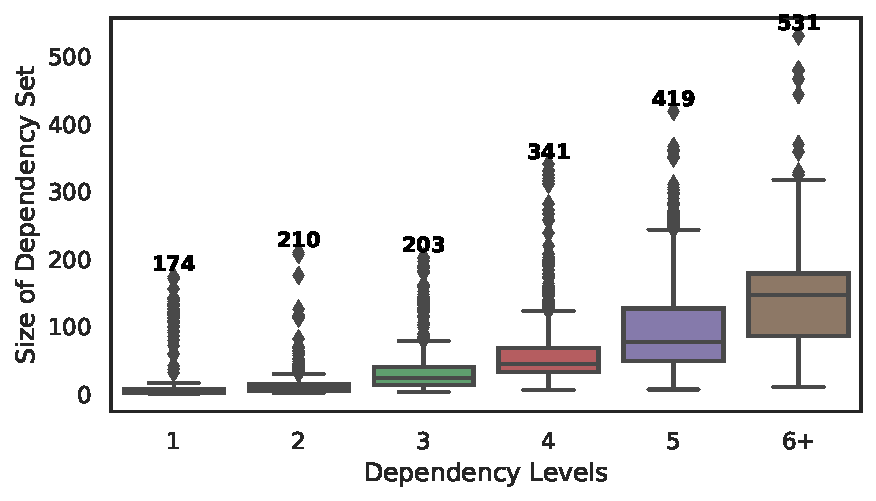
\includegraphics[width=0.8\linewidth]{chapters/ch3/figs/num_deps_levels.pdf}
    \caption{Number of dependencies on various dependency depths}%. The number on top of the box plots show the number of versioned packages at different exact dependency levels.}
    \label{ch3:fig:num_deps_levels}
\end{figure}

\paragraph{Towards Intelligent Software Composition Analysis}
A number of free and commercial software composition analysis (SCA) tools exist that analyze the open-source components of a project for security risks and license compliance. Each of them differs widely in terms of accuracy, the quality of the vulnerability database, and the level of granularity~\cite{imtiaz2021comparative}. For instance, OWASP DC~\cite{owaspdepchk} analyzes dependency files of a project and notifies developers if known vulnerabilities are present in the project's transitive dependencies. However, as mentioned earlier, this level of granularity suffers from imprecision, and it is also not helpful for developers to better assess and mitigate the potential risk of using vulnerable dependencies in their projects. Also, free tools like GitHub's Dependabot perform package-level analysis, though its fine-grained analysis feature is in the beta state for the Python ecosystem as of this writing~\cite{ghd}. Overall, we believe that the next generation of SCA tools should have at least these core features when analyzing vulnerabilities in projects: (1) dependency depth (2) callable-level analysis (3) providing users with a detailed description of what part of their code is affected by vulnerabilities by showing, for example, vulnerable call paths and required actions to mitigate the security risk.

\paragraph{Transitivity Matters}
Transitivity matters when analyzing projects' dependencies for the presence of vulnerabilities.
Considering the results of RQ2 and RQ4, many versioned packages are affected by known vulnerabilities in the \textit{transitive} dependencies no matter the granularity level, i.e., dependency- or callable-level. For developers, this means that updating direct dependencies may not eliminate the potential security threat by a vulnerability. It is suggested that developers use an SCA tool and integrate it into their workflow or continuous integration pipeline, which helps to frequently monitor the transitive dependencies of their projects for the presence of vulnerabilities and update them if needed. For the developers of SCA tools, it is essential to analyze the whole transitive dependency set of projects to improve the reliability of their tools. We believe that SCA tools are not practical or useful if they naively only consider direct dependencies.

\paragraph{Popularity}
Popular vulnerable projects do not necessarily have the largest impact on the ecosystem.
RQ3 shows that a security vulnerability in a popular package can potentially affect many other dependent packages.
This confirms previous results in the NPM ecosystem~\cite{zimmermann2019small}, which stated that several popular JavaScript packages (in)directly affect thousands of other packages.
However, this observation is based on a basic package-level analysis of transitive dependencies, which is not precise enough to show the \emph{true} impact of vulnerabilities in the ecosystem.
The results change, when analyzed on the method-level.
For instance, we found that a vulnerability, \texttt{CVE-2021-37137} in the popular Maven project \texttt{netty-codec-http} potentially affects 142K other packages when analyzed on the package level.
However, through a method-level analysis, we only found 90 versioned packages that were actually affected.
On the other hand, the {\tt CVE-2018-1000632} in the less popular Maven project {\tt dom4j} only affects 47K other packages on the package level, but we found 1,400+ actually affected packages through a method-level analysis.
These results imply that popularity might not be as good an indicator for ecosystem impact as originally thought.
Better strategies to identify the critical packages are required to protect ecosystems as a whole.

\paragraph{Expensive Analyses}
Running ecosystem-wide, fine-grained analyses are expensive.
While fine-grained analysis provides a new perspective in studying a software ecosystem, it can be very computationally expensive to analyze millions of projects.
In this study, we managed to analyze 3 million versioned Maven packages and study the effect of transitivity and granularity on vulnerability propagation in Maven. From our experience, ecosystem-wide fine-grained analysis requires costly, powerful machines and sufficient time to perform. Given the result of the RQ4, one insight that might be useful for future work is to consider a lower dependency level (e.g., 3 or 4) in call graph-based analysis assuming that a slight loss of recall/precision is acceptable. This also may potentially reduce the search space and computation time.

\section{Threats to Validity}\label{ch3:sec:threats}
In this section, we describe possible threats to the validity of the obtained results and findings and how we addressed them.

\paragraph{Dataset}
In this study, we gathered a Maven dataset that consists of 3M versioned packages over a period of one year (from 2021-2022). We chose to gather data for one year mainly for two reasons: (1) In our approach, we generate call graphs for fine-grained analysis, which can be expensive. For us, it is not computationally feasible to perform this step for the whole history of the Maven ecosystem, which has over 9.8M versioned packages~\cite{mvn22} as of this writing. (2) The main goal of this study is to show the effect of transitivity and granularity on vulnerability propagation via fine-grained analysis in Maven. Therefore, following the guidelines for empirical software engineering research~\cite{Felderer2020ContemporaryEM}, we believe that our sample size, 3M versioned packages, is sufficient to achieve the said goal.
With such a large sample size, we are very confident that our findings would also hold for the whole history of the Maven ecosystem.

%Implementation

\paragraph{Vulnerability mapping to package versions}
As described before, we analyze vulnerability constraints in security reports to find the affected versions of a package by a vulnerability. Based on our observation, vulnerability constraints often only specify an upper bound on the range of affected versions.
This may falsely render older releases as vulnerable. No trivial solution can address this limitation.
However, with callable-level analysis, we can check whether the vulnerable method even exists in the previous releases, which can automatically eliminate many incorrect cases.

\paragraph{Call graph analysis}
We configure \tool{OPAL} to use an Open-Package Assumption to identify entrypoints when generating call graphs.
%, as described in subsection~\ref{subsec:cg-gen}.
OPA prioritizes soundness over precision, meaning that call graphs might have spurious edges, which may lead to false positives when finding vulnerable call chains. However, we argue that, for security-focused analysis, false negatives can be more expensive and dangerous. If a method is falsely identified as safe to use, it can potentially harm its users and their organizations~\cite{hagberg2021using}. In contrast, false positives prevent users to use a method and they can also be reviewed manually by security experts if the needed functionality is costly to implement. Moreover, as pointed out by Nielsen et al.~\cite{nielsen2021modular}, for security-focused applications, a few false negatives are likely more desirable than a large number of false positives. 

In addition, our call graph analysis does not consider control flow when assessing the reachability of vulnerable code or methods. This means that a false positive alarm is produced if the required input to trigger the vulnerability is not provided~\cite{kang2022test}. 

\section{Summary}\label{ch3:sec:conclusion}
In this chapter, we have studied the effect of transitivity and granularity on how vulnerabilities propagate to projects via fine-grained analysis in the Maven ecosystem. The methodology of our study is based on resolving transitive dependencies, building whole-program call graphs, and performing reachability analysis, which allows us to study vulnerability propagation at both dependency and callable levels. Among our findings, we found that, for security-focused applications, it is important to consider transitive dependencies regardless of the granularity level to minimize the risk of security threats. Also, with the callable-level analysis, it is possible to provide a lower bound for the analysis of vulnerability propagation in the ecosystem and also overcome the over-approximation issue of the dependency-level analysis. Overall, the implication of our results suggests that call graph-based analysis seems to be a promising direction for future studies on software ecosystems.
\chapter{Type4Py: Practical Deep Similarity Learning-Based Type Inference for Python}
\label{ch:t4py}

\blfootnote{This chapter is based on the paper, Mir, A. M., Latoškinas, E., Proksch, S., \& Gousios, G., Type4py: Practical Deep Similarity Learning-based Type Inference for Python. In Proceedings of the 44th International Conference on Software Engineering (ICSE'22) (pp. 2241-2252).~\cite{mir2022type4py}.
}

\newcommand{\name}{\tool{Type4Py}}
\newcommand{\cmark}{\ding{51}}
\newcommand{\xmark}{\ding{55}}

\begin{abstract}
Dynamic languages, such as Python and Javascript, trade static typing for 
developer flexibility and productivity. Lack of static typing can cause run-time exceptions and is a
major factor for weak IDE support. To alleviate these issues, PEP 484 introduced
optional type annotations for Python. As retrofitting types to existing
codebases is error-prone and laborious, machine learning (ML)-based approaches have been proposed to
enable automatic type inference based on existing, partially annotated
codebases.
However, previous ML-based approaches are trained and evaluated on human-provided type annotations, 
which might not always be sound, and hence this may limit the practicality for real-world usage.
In this chapter, we present \name, a deep similarity learning-based hierarchical neural network model.
It learns to discriminate between similar and dissimilar types in a high-dimensional space, which results in clusters of types.
Likely types for arguments, variables, and return values can then be inferred through the nearest neighbor search.
Unlike previous work, we trained and evaluated our model on a \emph{type-checked} dataset and used mean reciprocal rank (MRR) to reflect the performance perceived by users.
The obtained results show that \name achieves an MRR of 77.1\%, which is a substantial improvement of 8.1\% and 16.7\% over the state-of-the-art approaches \tool{Typilus} and \tool{TypeWriter}, respectively. Finally, to aid developers with retrofitting types, we released a Visual Studio Code extension, which uses \name to provide ML-based type auto-completion for Python.
\end{abstract}

\newpage

\section{Introduction}
Over the past years, \emph{dynamically-typed} programming languages (DPLs) have become extremely popular among software developers.
The IEEE Spectrum ranks Python as the most popular programming language in 2021~\cite{ieeespec2019}.
It is known that \emph{statically-typed} languages are less error-prone~\cite{ray2014large} and that static types improve important quality aspects of software~\cite{gao2017type}, like the maintainability of software systems in terms of understandability, fixing type errors~\cite{hanenberg2014empirical}, and early bug detection~\cite{gao2017type}.
In contrast to that, dynamic languages such as Python and JavaScript allow rapid prototyping which potentially reduces development time~\cite{hanenberg2014empirical, stuchlik2011static}, but the lack of static types in dynamically-typed languages often leads to type errors, unexpected run-time behavior, and suboptimal IDE support.

To mitigate these shortcomings, the Python community introduced \emph{PEP 484}~\cite{van2014pep}, which adds optional static typing to Python 3.5 and newer.
Static type inference methods~\cite{hassan2018maxsmt, furr2009static} can be employed to support adding these annotations, which is otherwise a manual, cumbersome, and error-prone process~\cite{ore2018assessing}.
However, static inference is imprecise~\cite{pavlinovic2019leveraging}, caused by dynamic language features or by the required over-approximation of program behavior~\cite{madsen2015static}.
Moreover, static analysis is usually performed on full programs, including their dependencies, which is slow and resource-intensive.

To address these limitations of static type inference methods, researchers have recently employed \emph{Machine Learning} (ML) techniques for type prediction in dynamic languages~\cite{hellendoorn2018deep, malik2019nl2type, pradel2019typewriter, allamanis2020typilus}.
The experimental results of these studies show that ML-based type prediction approaches are more precise than static type inference methods or they can also work with static methods in a complementary fashion~\cite{pradel2019typewriter, allamanis2020typilus}. Despite the superiority of ML-based type prediction approaches, their type vocabulary is small and fixed-sized (i.e. 1,000 types). This limits their type prediction ability for user-defined and rare types. To solve this issue, Allamanis et al.~\cite{allamanis2020typilus} recently introduced \tool{Typilus} which does not constraint the type vocabulary size and it outperforms the other models with small-sized type vocabulary.

While the ML-based type inference approaches are effective, we believe that there are two main drawbacks in the recent previous work~\cite{pradel2019typewriter, allamanis2020typilus}:
\begin{itemize}
	\item The neural models are trained and evaluated on developer-provided type annotations, which are not always correct~\cite{ore2018assessing, rak2020python}. This might be a (major) threat to the validity of the obtained results. To address this, a type checker should be employed to detect and remove incorrect type annotations from the dataset.
	\item Although the proposed approaches~\cite{pradel2019typewriter, allamanis2020typilus} obtain satisfying performance for Top-10, it is important for an approach to give a correct prediction in Top-1 as developers tend to use the first suggestion by a tool~\cite{parnin2011automated}. Like the API recommendation research~\cite{liu2018effective, he2021pyart}, the Mean Reciprocal Rank (MRR) metric should also be used for evaluation, which \emph{partially} rewards an approach where the correct API is not in the Top-1 suggestion.
\end{itemize}

Motivated by the above discussion, we present \name, a type inference approach based on \emph{deep similarity learning} (DSL).
The proposed approach consists of an effective hierarchical neural network that maps programs into \emph{type clusters} in a high-dimensional feature space.
Similarity learning has, for example, been used in Computer Vision to discriminate human faces for verification~\cite{chopra2005learning}. Similarly, \name learns how to distinguish between different types through a DSL-based hierarchical neural network.
As a result, our proposed approach can not only handle a very large type vocabulary, but also it can be used in practice by developers for retrofitting type annotations.
In comparison with the state-of-the-art approaches, the experimental results show that \name obtains an MRR of 77.1\%,
which is 8.1\% and 16.7\% higher than \tool{Typilus}~\cite{allamanis2020typilus} and \tool{TypeWriter}~\cite{pradel2019typewriter}, respectively.

\smallskip
\noindent
Overall, this paper presents the following main contributions:
\begin{itemize}
	\item \name, a new DSL-based type inference approach.
	\item A \emph{type-checked} dataset with 5.1K Python projects and 1.2M type annotations. Invalid type annotations are removed from both training and evaluation.
%	\item Different from previous work~\cite{pradel2019typewriter, typilus}, we evaluate the type inference neural models with the MRR metric as well, which considers the rank of predicted type annotations.
	\item A Visual Studio Code extension~\cite{vscodet4py}, which provides ML-based type auto-completion for Python.
\end{itemize}

To foster future research, we publicly released the implementation of the \name model and its dataset on Zenodo.\footnote{https://doi.org/10.5281/zenodo.5913787}

The rest of the chapter is organized as follows. Section \ref{ch4:sec:rw} reviews related work on static and ML-based type inference. The proposed approach, \name, is described in Section \ref{ch4:sec:pa}. Section \ref{ch4:sec:data} gives details about the creation of the type-checked dataset for evaluation. The evaluation setup and empirical results are given in Section \ref{ch4:sec:es} and Section \ref{ch4:sec:eval}, respectively. Section \ref{ch4:sec:prac} describes the deployment of \name and its usage in Visual Studio Code. Section \ref{ch4:sec:discuss} discusses the obtained results and gives future directions. Finally, we summarize our work in Section \ref{ch4:sec:sum}.

\newpage

\section{Related Work}\label{ch4:sec:rw}

\begin{table*}[!t]
	\centering
	\caption{Comparison between \name and other learning-based type inference approaches}
	\label{tab:comp-learning-appr}
	\begin{threeparttable}
	\resizebox{\textwidth}{!}{\begin{tabular}{c c c c c c c c c c}
		\toprule
		\multirow{2}{*}{Approach} & \multirow{2}{*}{Size of type vocabulary} & \multirow{2}{*}{ML model} & \multicolumn{3}{c}{Type hints} & &  \multicolumn{3}{c}{Supported Predictions} \\
		\cmidrule{4-6} \cmidrule{8-10}
		& & & Contextual & Natural & Logical & & Argument & Return & Variable \\
		\midrule
		\textbf{\name} & Unlimited & HNN (2x RNNs) & \cmark & \cmark & \xmark & & \cmark & \cmark & \cmark \\
		JSNice \cite{raychev2015predicting} & 10+ & CRFs & \cmark & \cmark & \xmark &&  \cmark & \xmark & \xmark \\
		Xu et al. \cite{xu2016python} & - & PGM & \xmark & \cmark & \cmark & & \xmark & \xmark & \cmark \\
		DeepTyper \cite{hellendoorn2018deep} & 10K+ & biRNN & \cmark & \cmark & \xmark & & \cmark & \cmark & \cmark \\
		NL2Type \cite{malik2019nl2type} & 1K & LSTM & \xmark & \cmark & \xmark &  & \cmark & \cmark & \xmark \\
		TypeWriter \cite{pradel2019typewriter} & 1K & HNN (3x RNNs) & \cmark & \cmark & \xmark & & \cmark & \cmark & \xmark  \\
		LAMBDANET \cite{wei2019lambdanet} & 100\tnote{a} & GNN & \cmark & \cmark & \cmark & & \xmark & \xmark & \cmark \\
		OptTyper \cite{pandi2020opttyper} & 100 & LSTM & \xmark & \cmark & \cmark &  & \cmark & \cmark & \xmark \\
		Typilus \cite{allamanis2020typilus} & Unlimited & GNN & \cmark & \cmark & \xmark  & & \cmark & \cmark & \cmark \\
		TypeBert \cite{jesse2021learning} & 40K & BERT & \cmark & \cmark & \xmark & & \cmark & \cmark & \cmark \\
		\bottomrule
	\end{tabular}}
    \begin{tablenotes}
    	\item[a] {\footnotesize Note that LAMBDANET's pointer network model enables to predict user-defined types \\ outside its fixed-size type vocabulary.}
    \end{tablenotes}
    \end{threeparttable}
\end{table*}

\paragraph{Type checking  and inference for Python}
In 2014, the Python community introduced a type hints proposal \cite{van2014pep} that describes adding optional type annotations to Python programs. A year later, Python 3.5 was released with optional type annotations and the \textit{mypy} type checker \cite{lehtosalo2017mypy}. This has enabled gradual typing of existing Python programs and validating added type annotations. Since the introduction of type hints proposal, other type checkers have been developed such as \textit{PyType} \cite{pytype}, \textit{PyRight} \cite{pyright}, and \textit{Pyre} \cite{pyre}.

A number of research works proposed type inference algorithms for Python \cite{salib2004faster, maia2012static, hassan2018maxsmt}. These are static-based approaches that have a pre-defined set of rules and constraints. As previously mentioned, static type inference methods are often imprecise \cite{pavlinovic2019leveraging}, due to the dynamic nature of Python and the over-approximation of programs' behavior by static analysis \cite{madsen2015static}.

\paragraph{Learning-based type inference} In 2015, Rachev et al.~\cite{raychev2015predicting} proposed JSNice, a probabilistic model that predicts identifier names and type annotations for JavaScript using conditional random fields (CRFs). The central idea of JSNice is to capture relationships between program elements in a dependency network.
However, the main issue with JSNice is that its dependency network cannot consider a wide context within a program or a function.

Xu et al.~\cite{xu2016python} adopt a probabilistic graphical model (PGM) to predict variable types for Python. Their approach extracts several uncertain type hints such as attribute access, variable names, and data flow between variables. Although the probabilistic model of Xu et al.~\cite{xu2016python} outperforms static type inference systems, their proposed system is slow and lacks scalability.

Considering the mentioned issue of JSNice, Hellendoorn et al.~\cite{hellendoorn2018deep} proposed DeepTyper, a sequence-to-sequence neural network model that was trained on an aligned corpus of TypeScript code. The DeepTyper model can predict type annotations across a source code file by considering a much wider context. Yet DeepTyper suffers from inconsistent predictions for the token-level occurrences of the same variable. Malik et al.~\cite{malik2019nl2type} proposed NL2Type, a neural network model that predicts type annotations for JavaScript functions. The basic idea of NL2Type is to leverage the natural language information in the source code such as identifier names and comments. The NL2Type model is shown to outperform both the JSNice and DeepTyper at the task of type annotations prediction~\cite{malik2019nl2type}.

Motivated by the NL2Type model, Pradel et al.~\cite{pradel2019typewriter} proposed the TypeWriter model which infers type annotations for Python. TypeWriter is a deep neural network model that considers both code context and natural language information in the source code. Moreover, TypeWriter validates its neural model's type predictions by employing a combinatorial search strategy and an external type checker. Wei et al.~\cite{wei2019lambdanet} introduced LAMBDANET, a graph neural network-based type inference for TypeScript. Its main idea is to create a type dependency graph that links to-be-typed variables with logical constraints and contextual hints such as variables assignments and names. For type prediction, LAMBDANET employs a pointer-network-like model which enables the prediction of unseen user-defined types. The experimental results of Wei et al.~\cite{wei2019lambdanet} show the superiority of LAMBDANET over DeepTyper.

Given that the natural constraints such as identifiers and comments are an uncertain source of information, Pandi et al.~\cite{pandi2020opttyper} proposed OptTyper which predicts types for the TypeScript language. The central idea of their approach is to extract deterministic information or logical constraints from a type system and combine them with the natural constraints in a single optimization problem. This allows OptTyper to make a type-correct prediction without violating the typing rules of the language. OptTyper has been shown to outperform both LAMBDANET and DeepTyper~\cite{pandi2020opttyper}.

Except for LAMBDANET, all the discussed learning-based type inference methods employ a (small) fixed-size type vocabulary, e.g., 1,000 types. This hinders their ability to infer user-defined and rare types. To address this, Allamanis et al.~\cite{allamanis2020typilus} proposed Typilus, which is a graph neural network (GNN)-based model that integrates information from several sources such as identifiers, syntactic patterns, and data flow to infer type annotations for Python. Typilus is based on metric-based learning and learns to discriminate similar to-be-typed symbols from different ones. However, Typilus requires a sophisticated source code analysis to create its graph representations, i.e. data flow analysis. Very recently, inspired by "Big Data", Jesse et al. ~\cite{jesse2021learning} presented TypeBert, a pre-trained BERT model with simple token-sequence representation. Their empirical results show that TypeBert generally outperforms LAMBDANET. The differences between \name and other learning-based approaches are summarized in Table \ref{tab:comp-learning-appr}.

\newpage
\section{Proposed Approach}\label{ch4:sec:pa}

\begin{figure}[!t]
	\centering
	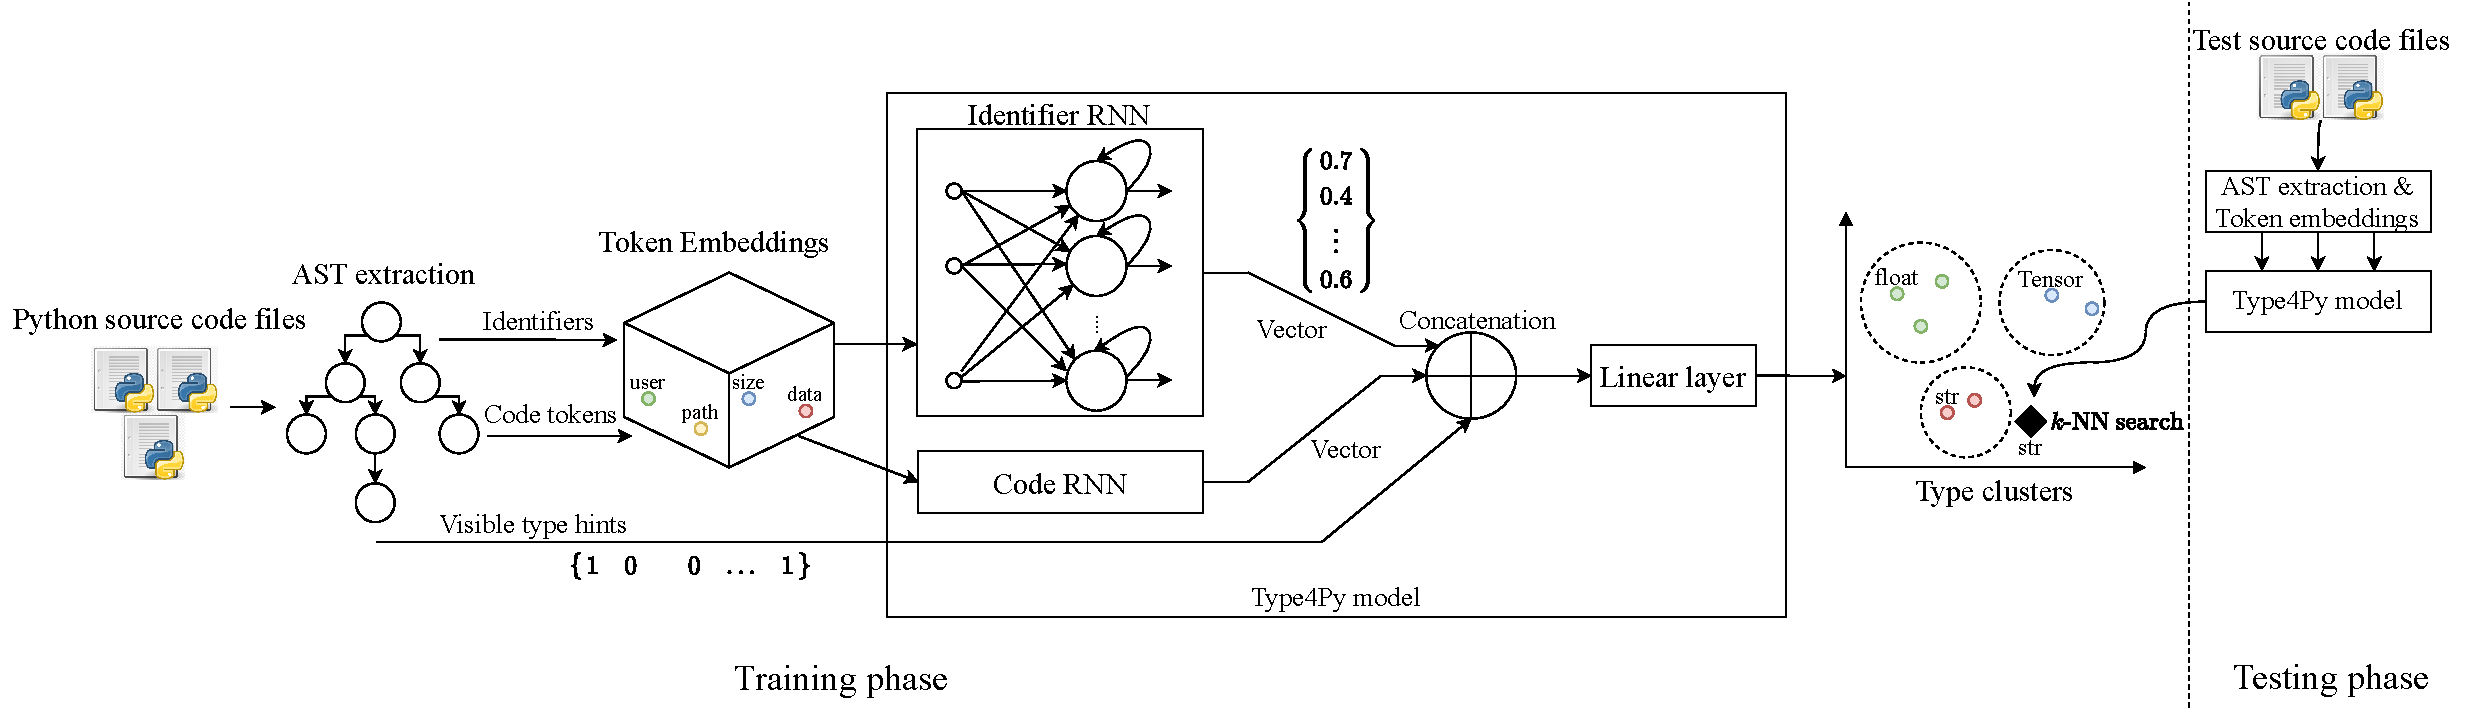
\includegraphics[width=\linewidth]{chapters/ch4/figs/Type4Py-Overview.pdf}
	\caption{Overview of \name approach}
	\label{ch4:fig:overview-approach}
\end{figure}

This section presents the details of \name by going through the different steps of the pipeline that is illustrated in the overview of the proposed approach in Figure~\ref{ch4:fig:overview-approach}.
We first describe how we extract type hints from Python source code and then how we use this information to train the neural model.

\subsection{Type Hints}
We extract the Abstract Syntax Tree (AST) from Python source code files. By traversing the nodes of ASTs, we obtain type hints that are valuable for predicting types of function arguments, variables, and return types. The obtained type hints are based on natural information, code context, and import statements which are described in this section.

\paragraph{Natural Information}
As indicated by the previous work~\cite{hindle2012naturalness, malik2019nl2type}, source code contains useful and informal natural language information that is considered as a source of type hints. In DPLs, developers tend to name variables and functions' arguments after their expected type~\cite{milojkovic2017exploiting}. Based on this intuition, we consider identifier names as the main source of natural information and type hint. Specifically, we extract the name of functions ($N_{f}$) and their arguments ($N_{args}$) as they may provide a hint about the return type of functions and the type of functions' arguments, respectively. We also denote a function's argument as $N_{arg}$ hereafter. For variables, we extract their names as denoted by $N_{v}$.

\paragraph{Code Context}
We extract all uses of an argument in the function body as a type hint.
This means that the complete statement, in which the argument is used, is included as a sequence of tokens. Similarly, we extract all uses of a variable in its current and inner scopes.
Also, all the return statements inside a function are extracted as they may contain a hint about the return type of the function.

\paragraph{Visible type hints (VTH)}
In contrast to previous work that only analyzed the direct imports~\cite{pradel2019typewriter}, we recursively extract all the import statements in a given module and its transitive dependencies.
We build a dependency graph for all imports of user-defined classes, type aliases, and \texttt{NewType} declarations
For example, if module \texttt{A} imports \texttt{B.Type} and \texttt{C.D.E}, the edges (\texttt{A}, \texttt{B.Type}) and (\texttt{A}, \texttt{C.D.E}) will be added to the graph.
We expand wildcard imports like \texttt{from foo import *} and resolve the concrete type references.
We consider the identified types as \emph{visible} and store them with their fully-qualified name to reduce ambiguity. For instance, \texttt{tf.Tensor} and \texttt{torch.Tensor} are different types.
Although the described inspection-based approach is slower than a pure AST-based analysis, our ablation analysis shows that VTHs substantially improve the performance of \name (subsection~\ref{subsec:abalation}).

\subsection{Vector Representation}
In order for a machine learning model to learn from type hints, they are represented as real-valued vectors. The vectors preserve semantic similarities between similar words. To capture those, a word embedding technique is used to map words into a $d$-dimensional vector space, $\mathbb{R}^{d}$. Specifically, we first preprocess extracted identifiers and code contexts by applying common Natural Language Processing (NLP) techniques. This preprocessing step involves tokenization, stop word removal, and lemmatization~\cite{JurafskyNLP}. Afterwards, we employ Word2Vec \cite{mikolov2013distributed} embeddings to train a code embedding $E_{c}: w_{1},\dots,w_{l} \to \mathbb{R}^{l \times d}$ for both code context and identifier tokens, where $w_{i}$ and $l$ denote a single token and the length of a sequence, respectively. In the following, we describe the vector representation of all the three described type hints for both argument types and return types.

\paragraph{Identifiers} Given an argument's type hints, the vector sequence of the argument is represented as follows:
\begin{equation*}
E_{c}(N_{arg}) \, \circ s \, \circ E_{c}(N_{f}) \, \circ E_{c}(N_{args})
\end{equation*}
where $\circ$ concatenates and flattens sequences, and $s$ is a separator\footnote{The separator is a vector of ones with appropriate dimension.}. For a return type, its vector sequence is represented as follows:
\begin{equation*}
E_{c}(N_{f}) \, \circ s \, \circ E_{c}(N_{args})
\end{equation*}
Last, a variable's identifier is embedded as $E_{c}({N_{v}})$.

\paragraph{Code contexts} For function arguments and variables, we concatenate the sequences of their usages into a single sequence. Similarly, for return types, we concatenate all the return statements of a function into a single sequence. To truncate long sequences, we consider a window of $n$ tokens at the center of the sequence (default $n=7$). Similar to identifiers, the function embedding $E_{c}$ is used to convert code contexts sequences into a real-valued vector.

\paragraph{Visible type hints} Given all the source code files, we build a fixed-size vocabulary of visible type hints. The vocabulary covers the majority of all visible type occurrences. Because most imported visible types in Python modules are built-in primitive types such as \texttt{List}, \texttt{Dict}, and their combinations. If a type is out of the visible type vocabulary, it is represented as a special \texttt{other} type. For function arguments, variables, and return types, we create a sparse binary vector of size $T$ whose elements represent a type. An element of the binary vector is set to one if and only if its type is present in the vocabulary. Otherwise, the \texttt{other} type is set to one in the binary vector.

\subsection{Neural Model}
The neural model of our proposed approach employs a hierarchical neural network (HNN), which consists of two recurrent neural networks (RNNs)~\cite{williams1989learning}. HNNs are well-studied and quite effective for text and vision-related tasks~\cite{liu2020hienn, zheng2019hierarchical, du2015hierarchical}. In the case of type prediction, intuitively, HNNs can capture different aspects of identifiers and code context. In the neural architecture (see Fig. \ref{ch4:fig:overview-approach}), the two RNNs are based on long short-term memory (LSTM) units~\cite{hochreiter1997long}. Here, we chose LSTMs units as they are effective for capturing long-range dependencies~\cite{goodfellow2016deep}. Also, LSTM-based neural models have been applied successfully to NLP tasks such as sentiment classification~\cite{rao2018lstm}. Formally, the output $h_{i}^{(t)}$ of the $i$-th LSTM unit at the time step $t$ is defined as follows:
% this comment eliminates extensive whitespace before equation
\begin{equation}
h_{i}^{(t)} = \tanh(s_{i}^{t}) \, \sigma\left( b_{i} +  \sum\limits_{j}{U_{i,j}x_{j}^{(t)} + \sum\limits_{j}{W_{i,j}h_{j}^{(t-1)}}} \right)
\end{equation}

\noindent which has sigmoid function $\sigma$, current input vector $x_{j}$, unit state $s_{i}^{t}$ and has model parameters $W$, $U$, $b$ for its recurrent weights, input weights and biases~\cite{goodfellow2016deep}. The two hierarchical RNNs allow capturing different aspects of input sequences from identifiers and code tokens. The captured information is then summarized into two single vectors, which are obtained from the final hidden state of their corresponding RNN. The two single vectors from RNNs are concatenated with the visible type hints vector and the resulting vector is passed through a fully-connected linear layer.

In previous work~\cite{pradel2019typewriter, malik2019nl2type}, the type prediction task is formulated as a classification problem. As a result, the linear layer of their neural model outputs a vector of size 1,000 with probabilities over predicted types. Therefore, the neural model predicts \textit{unkonwn} if it has not seen a type in the training phase. To address this issue, we formulate the type prediction task as a Deep Similarity Learning problem~\cite{chopra2005learning, liao2017triplet}. By using the DSL formulation, our neural model learns to map argument, variable, return types into real continuous space, called \textit{type clusters} (also known as type space in~\cite{allamanis2020typilus}). In other words, our neural model maps similar types (e.g. \texttt{str}) into its own type cluster, which should be as far as possible from other clusters of types. Unlike the previous work~\cite{pradel2019typewriter, malik2019nl2type}, our proposed model can handle a very large type vocabulary.

To create the described type clusters, we use \textit{Triplet loss}~\cite{cheng2016person} function which is recently used for computer vision tasks such as face recognition~\cite{cheng2016person}. By using the Triplet loss, a neural model learns to discriminate between similar samples and dissimilar samples by mapping samples into their own clusters in the continuous space. In the case of type prediction, the loss function accepts a type $t_{a}$, a type $t_{p}$ same as $t_{a}$, and a type $t_{n}$ which is different than $t_{a}$. Given a positive scalar margin $m$, the Triplet loss function is defined as follows:
% this comment eliminates extensive whitespace before equation
\begin{equation}\label{eq:triplet}
L(t_{a}, t_{p}, t_{n}) = max(0, m + \left\| t_{a} - t_{p} \right\| - \left\| t_{a} - t_{n} \right\|)
\end{equation}

The goal of the objective function $L$ is to make $t_{a}$ examples closer to the similar examples $t_{p}$ than to $t_{n}$ examples. We use the Euclidean metric to measure the distance of $t_{a}$ with $t_{p}$ and $t_{n}$.

At prediction time, we first map a query example $t_{q}$ to the type clusters. The query example $t_{q}$ can be a function's argument, the return type of a function or a variable. Then we find the $k$-nearest neighbor (KNN)~\cite{cover1967nearest} of the query example $t_{q}$. Given the $k$-nearest examples $t_{i}$ with a distance $d_{i}$ from the query example $t_{q}$, the probability of $t_{q}$ having a type $t^{\prime}$ can be obtained as follows:
% this comment eliminates extensive whitespace before equation
\begin{equation}
P(t_{q}: t^{\prime}) = \frac{1}{N} \sum\limits_{i}^{k}{\frac{\mathbb{I}(t_{i} = t^{\prime} )}{(d_{i} + \varepsilon)^{2} }}
\end{equation}

where $\mathbb{I}$ is the indicator function, $N$ is a normalizing constant, and $\varepsilon$ is a small scalar (i.e. $\varepsilon = 10^{-10}$).

\section{Dataset}\label{ch4:sec:data}
For this work, we have created a new version of our ManyTypes4Py dataset~\cite{mt4py2021}, i.e., v0.7. The rest of this section describes the creation of the dataset. To find Python projects with type annotations, on Libraries.io, we searched for projects that depend on the \texttt{mypy} package~\cite{mypy}, i.e., the official and most popular type checker for Python. Intuitively, these projects are more likely to have type annotations. The search resulted in 5.2K Python projects that are available on GitHub. Initially, the dataset has 685K source files and 869K type annotations.

\subsection{Code De-duplication}
On GitHub, Python projects often have file-level duplicates~\cite{lopes2017dejavu} and also code duplication has a negative effect on the performance of ML models when evaluating them on unseen code samples~\cite{allamanis2018adverse}. Therefore, to de-duplicate the dataset, we use our code de-duplication tool, CD4Py~\cite{cd4py}. It uses term frequency-inverse document (TF-IDF) \cite{manning2008introduction} to represent a source code file as a vector in $\mathbb{R}^{n}$ and employs KNN search to find clusters of similar duplicate files. While assuming that the similarity is transitive \cite{allamanis2018adverse}, we keep a file from each cluster and remove all other identified duplicate files from the dataset. Using the described method, we removed around 400K duplicate files from the dataset.

\subsection{Augmentation}
Similar to the work of Allamanis et al.~\cite{allamanis2020typilus}, we have employed a static type inference tool, namely, Pyre~\cite{pyre} v0.9.0 to augment our initial dataset with more type annotations. However, we do note that we could only infer the type of variables using Pyre's \code{query} command. In our experience, the query command could not infer the type of arguments and return types. The command accepts a list of files and returns JSON files containing type information.

Thanks to Pyre's inferred types, the dataset has now 3.3M type annotations in total. To demonstrate the effect of using Pyre on the dataset, Figure \ref{ch4:fig:dataset-type-annot-cove-pyre} shows the percentage of type annotation coverage for source code files with/without using Pyre. After using Pyre, of 288,760 source code files, 65\% of them have more than 40\% type annotation coverage.

\begin{figure}[!t]
	\centering
	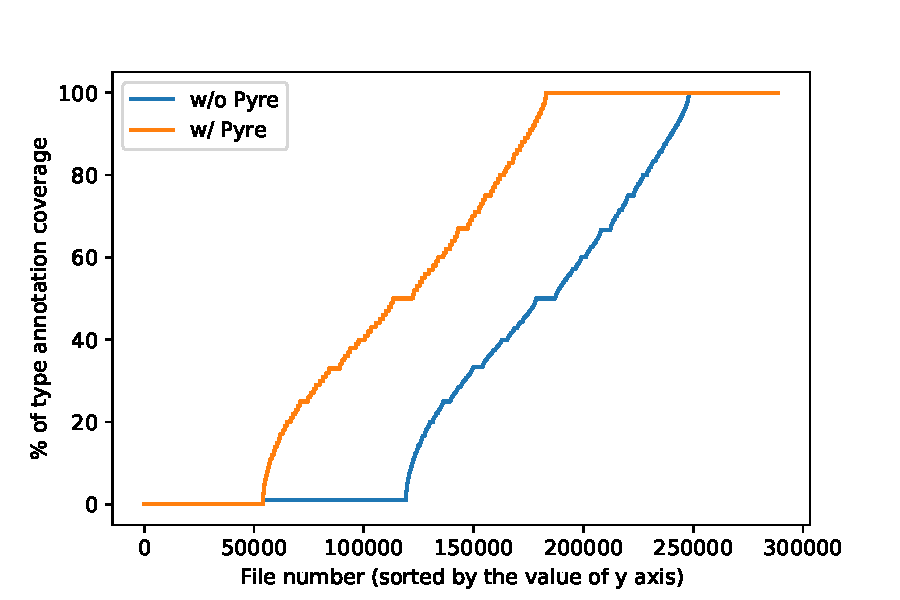
\includegraphics[width=\linewidth]{chapters/ch4/figs/type_cove_f_pyre.pdf}
	\caption{The effect of using Pyre on the type annotation coverage of source code files}
	\label{ch4:fig:dataset-type-annot-cove-pyre}
\end{figure}

\subsection{Type Checking}
Recent studies show that developer-provided types rarely type-check and Python projects may contain type-related defects~\cite{ore2018assessing, rak2020python, khan2021empirical}. Therefore, we believe that it is essential to type-check the dataset to eliminate noisy ground truth (i.e. incorrect type annotations). Not only noisy ground truth can be considered a threat to the validity of results but also it may make the discrimination of types in type clusters more difficult~\cite{garcia2015effect}. To clean the dataset from noisy ground truth, we perform basic analysis as follows:
\begin{itemize}
	\item First, we use mypy to type-check 288,760 source files in the dataset. Of which, 184,752 source files are successfully type-checked.
	\item Considering the remaining 104,008 source files, for further analysis, we ignore source files that cannot be type-checked further by mypy due to syntax error or other fatal exceptions. This amounts to 63,735 source files in the dataset.
	\item Given 40,273 source files with type errors, we remove one type annotation at a time from a file and run mypy. If it type-checks, we include the file. Otherwise, we continue this step up to 10 times. This basic analysis fixes 16,861 source files with type errors, i.e, 42\% of the given set of files.
\end{itemize}

\begin{table}[!t]
	\centering
	\caption{Characteristics of the dataset used for evaluation}
	\label{ch4:tab:dataset}
	\begin{threeparttable}
		\begin{tabular}{@{}ll@{}}
			\toprule
			Metrics\tnote{a,b} & Our dataset \\
			\midrule
			Repositories & 5,092 \\
			Files & 201,613 \\
			Lines of code\tnote{c} & 11.9M \\
			\midrule
			Functions & 882,657 \\
			...with return type annotations & 94,433 (10.7\%) \\
			\midrule
			Arguments & 1,558,566 \\
			...with type annotations & 128,363 (14.5\%) \\
			\midrule
			Variables & 2,135,361 \\
			...with type annotations & 1,023,328 (47.9\%) \\
			\midrule
			Types & 1,246,124 \\
			...unique & 60,333 \\
			\bottomrule
		\end{tabular}
		\begin{tablenotes}[flushleft]
			\item[a] {\footnotesize Metrics are counted after the ASTs extraction phase of our pipeline.}
			%\item[b] {\footnotesize Pyre's inferred types are considered in the metrics as well.}
			\item[c] {\footnotesize Comments and blank lines are ignored when counting lines of code.}
		\end{tablenotes}
	\end{threeparttable}
\end{table}

\begin{table}
	\centering
	\caption{Number of data points for train, validation and test sets}
	\label{ch4:tab:datapoints}
	\begin{tabular}{@{}l l l l@{}}
		\toprule
		%		& \multicolumn{3}{@{}c@{}}{Our dataset} \\
		%		\cmidrule{2-4}
		& Argument type & Return type & Variable type\\
		\midrule
		Training & 90,114  & 37,803 & 426,235 \\
		Validation & 9,387 & 3,932 & 48,518 \\
		Test & 24,121 & 10,444 & 118,319 \\
		\midrule
		Total &  108,888 (16.06\%) & 45,667 (6.74\%) & 523,271 (77.20\%) \\
		\bottomrule
		%		\vspace{6pt}\\
		%		\toprule
		%		& \multicolumn{2}{c}{Typilus' dataset \cite{allamanis2020typilus} } \\
		%		\cmidrule{2-3}
		%		& Argument type & Return type  \\
		%		\midrule
		%		Training & 60,574  & 23,227  \\
		%		Validation & 5,647  & 2,243 \\
		%		Test & 16,964 & 6,349 \\
		%		\midrule
		%		Total & 83,185 (72.3\%) & 31,819 (27.7\%) \\
		%		\bottomrule
	\end{tabular}
\end{table}

\subsection{Dataset Characteristics}
% Similar to \cite{allamanis2020typilus}, we used \texttt{PyType} to infer type annotations for the projects of the Typilus' dataset.
Table \ref{ch4:tab:dataset} shows the characteristics of our dataset after code de-duplication, augmentation, and type-checking. In total, there are more than 882K functions with around 1.5M arguments. Also, the dataset has more than 2.1M variable declarations. Of which, 48\% have type annotations.

Figure \ref{ch4:fig:top_10_types} shows the frequency of top 10 most frequent types in our dataset. It can be observed that types follow a long-tail distribution. Unsurprisingly, the top 10 most frequent types amount to 59\% of types in the dataset. Lastly, we randomly split the dataset by files into three sets: 70\% training data, 10\% validation data, and 20\% test data. Table \ref{ch4:tab:datapoints} shows the number of data points for each of the three sets.

\subsection{Pre-processing}
Similar to the previous work~\cite{pradel2019typewriter, allamanis2020typilus}, before training ML models, we have performed several pre-processing steps:

\begin{itemize}
	\item Trivial functions such as \code{\_\_str\_\_} and \code{\_\_len\_\_} are not included in the dataset. The return type of this kind of functions is straightforward to predict, i.e., \code{\_\_len\_\_} always returns \code{int}, and would blur the results.
	\item We excluded \code{Any} and \code{None} type annotations as it is not helpful to predict these types.
	\item We performed a simple type aliasing resolving to make type annotations of the same kind consistent. For instance, we map \code{[]} to \code{List}, \code{\{\}} to \code{Dict}, and \code{Text} to \code{str}.
	\item We resolved qualified names for type annotations. For example, \code{array} is resolved to \code{numpy.array}. This makes all the occurrences of a type annotation across the dataset consistent.
	\item Same as the work of Allamanis et al.~\cite{allamanis2020typilus}, we rewrote the components of a base type whose nested level is greater than 2 to \code{Any}. For instance, we rewrite \\ \code{List[List[Tuple[int]]]} to \code{List[List[Any]]]}. This removes very rare types or outliers.
\end{itemize}

\begin{figure}[!t]
	\centering
	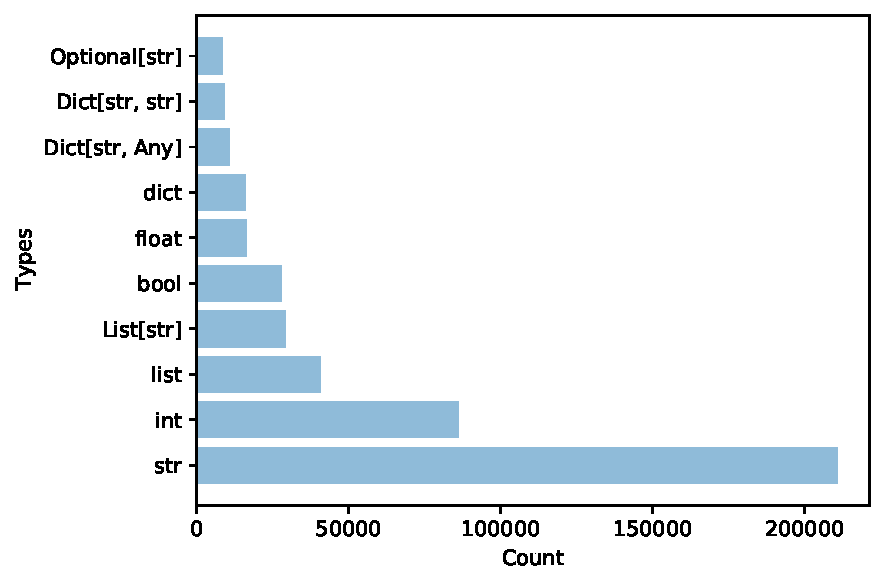
\includegraphics[width=\linewidth]{chapters/ch4/figs/top-10-most-frequent-types.pdf}
	\caption{Top 10 most frequent types (\texttt{Any} and \texttt{None} types are excluded)}
	\label{ch4:fig:top_10_types}
\end{figure}

\section{Evaluation Setup}\label{ch4:sec:es}
In this section, we describe the baseline models, the implementation details and the training of the neural models. Lastly, we explain evaluation metrics to quantitatively measure the performance of ML-based type inference approaches.

\subsection{Baselines}
We compare \name to Typilus~\cite{allamanis2020typilus} and TypeWriter~\cite{pradel2019typewriter}, which are recent state-of-the-art ML-based type inference approaches for Python. Considering Table \ref{tab:comp-learning-appr}, \name has an HNN-based neural model whereas Typilus's neural model is GNN-based. However, Typilus has the same prediction abilities as \name and has no limitation on the size of type vocabulary which makes it an obvious choice for comparison. Compared with \name, TypeWriter has two main differences. First, TypeWriter's type vocabulary is small and pre-defined (i.e. 1,000 types) at training time. Second, TypeWriter cannot predict the type of variables, unlike \name and Typilus.

\subsection{Implementation Details and Environment Setup}
\label{ch4:sub:implementation}
We implemented \name and TypeWriter in Python 3 and its ecosystem. We extract the discussed type hints from ASTs using LibSA4Py~\cite{libsa4py}. The data processing pipeline is parallelized by employing the \textit{joblib} package. We use NLTK \cite{loper2002nltk} for performing standard NLP tasks such as tokenization and stop work removal. To train the Word2Vec model, the \textit{gensim} package is used. For the neural model, we used bidirectional LSTMs \cite{schuster1997bidirectional} in the PyTorch framework \cite{paszke2019pytorch} to implement the two RNNs. Lastly, we used the Annoy\cite{annoy} package to perform a fast and approximate nearest neighbor search. For Typilus, we used its public implementation on GitHub \cite{typilus}.

We performed all the experiments on a Linux operating system (Ubuntu 18.04.5 LTS).
The computer had an AMD Ryzen Threadripper 1920X with 24 threads (@3.5GHz), 64 GB of RAM, and two NVIDIA GeForce RTX 2080 TIs.

\begin{table}[!t]
	\caption{Value of hyperparameters for neural models}
	\label{ch4:tab:hyperp}
	\begin{threeparttable}\begin{tabular}{@{}lrrr@{}}
				\toprule
				Hyperparameter &  \name & TypeWriter & Typilus \\
				\midrule
				Word embedding dimension (i.e. $d$) & 100 & 100 & N/A \\
				Size of visible type hints vocabulary (i.e. $T$) & 1024 & 1024 & N/A \\
				LSTM hidden nodes & 256 & 256 & N/A \\
				GNN hidden nodes & N/A & N/A & 64 \\
				Dimension of linear layer's output & 1536 & 1000 & N/A \\
				Number of LSTM's layers & 1 & 1 & N/A \\
				Learning rate & 0.002 & 0.002 & 0.00025 \\
				Dropout rate & 0.25 & 0.25 & 0.1 \\
				Number of epochs & 25 & 25 & 500\tnote{a} \\
				Batch size & 5864 & 4096 & N/A \\
				Value of $k$ for nearest neighbor search & 10 & N/A & 10 \\
				Tripet loss' margin value (i.e. $m$) & 2.0 & N/A & 2.0 \\
				\midrule
				Model's trainable parameters & 4.6M & 4.7M & 650K \\
				\bottomrule
			\end{tabular}
			\begin{tablenotes}
				\item[a] {\footnotesize The model stopped at epoch 38 due to the early stopping technique.}
			\end{tablenotes}
	\end{threeparttable}
\end{table}

\subsection{Training}
To avoid overfitting the train set, we applied the Dropout regularization \cite{srivastava2014dropout} to the input sequences except for the visible types. Also, we employed the Adam optimizer \cite{kingma2014adam} to minimize the value of the Triplet loss function. For both \name and TypeWriter, we employed the data parallelism feature of PyTorch to distribute training batches between the two GPUs with a total VRAM of 22 GB.  For the \name model, given 554K training samples, a single training epoch takes around 4 minutes. It takes 7 seconds for the TypeWriter model providing that its training set contains 127K training samples\footnote{Note that TypeWriter uses only argument and return samples as it lacks the variable prediction ability.}. Aside from the training sample size, \name is a DSL-based model and hence it has to predict the output of three data points for every single training batch (see Eq. \ref{eq:triplet}). Typilus completes a single training epoch in around 6 minutes\footnote{The public implementation of Typilus does not take advantage of our two GPUs.}. For all the neural models, the validation set is used to find the optimal number of epochs for training. The value of the neural models' hyperparameters is reported in Table \ref{ch4:tab:hyperp}.

\subsection{Evaluation Metrics}
We measure the type prediction performance of an approach by comparing the type prediction $t_{p}$ to the ground truth $t_{g}$ using two criteria originally proposed by Allamanis et al.~\cite{allamanis2020typilus}:

\begin{description}
	%
	\item[Exact Match:] $t_{p}$ and $t_{g}$ are exactly the same type.
	%
	\item[Base Type Match:] ignores all type parameters and only matches the base types.
	%That is, it matches the outermost of a parametric type.
	For example, \code{List[str]} and \code{List[int]} would be considered a match.
	%
\end{description}

In addition to these two criteria, as stated earlier, we opt for the MRR metric~\cite{manning2008introduction}, since the neural models predict a list of types for a given query. The MRR of multiple queries $Q$ is defined as follows:
\begin{equation}
MRR = \frac{1}{|Q|}\sum_{i=1}^{|Q|}{\frac{1}{r_{i}}}
\end{equation}
The MRR metric partially rewards the neural models by giving a score of $\frac{1}{r_{i}}$ to a prediction if the correct type annotation appears in rank $r$. Like Top-1 accuracy, a score of 1 is given to a prediction for which the Top-1 suggested type is correct. Hereafter, we refer to the MRR of the Top-$n$ predictions as MRR@$n$. We evaluate the neural models up to the Top-10 predictions as it is a quite common methodology in the evaluation of ML-based models for code~\cite{ he2021pyart, allamanis2020typilus, pradel2019typewriter}.

Similar to the evaluation methodology of Allamanis et al.~\cite{allamanis2020typilus}, we consider types that we have seen more than 100 times in the train set as \emph{common} or \emph{rare} otherwise. Additionally, we define the set of \emph{ubiquitous} types, i.e., $\{\texttt{str}, \texttt{int}, \texttt{list}, \texttt{bool}, \texttt{float}\}$. These types are among the top 10 frequent types in the dataset (see Fig.~\ref{ch4:fig:top_10_types}) and they are excluded from the set of common types. Furthermore, Unlike \name and Typilus, TypeWriter predicts \code{unknown} if the expected type is not present in its type vocabulary. Thus, to have a valid comparison with the other two approaches, we consider \code{other} predictions by TypeWriter in the calculation of evaluation metrics.

\newpage

\section{Evaluation}
\label{ch4:sec:eval}
% \NewDocumentCommand\RQ{m}{RQ$_{#1}$}

To evaluate and show the effectiveness of \name, we focus on the following research questions.

\begin{description}[noitemsep]
	\item[\RQ{1}] What is the general type prediction performance of \name? 
	%	\item[\RQ{2}] How does \name perform while considering different top-$n$ predictions?
	\item[\RQ{2}] How does \name perform while considering different predictions tasks?
	\item[\RQ{3}] How do each proposed type hint and the size of type vocabulary contribute to the performance of \name?
	%\item[\RQ{4}] How effective is \name in terms of training and inference speed?
	%\item[\RQ{5}] How does \name compare qualitatively to the other approaches?
\end{description}

\begin{table*}[!t]
	\centering
	\caption{Performance evaluation of the neural models considering different top-$n$ predictions}
	\label{ch4:tab:top-n}
	   \begin{threeparttable}
	\resizebox{\textwidth}{!}{\begin{tabular}{@{}l l c c c c c c c c c @{}}
		\toprule
		\multirow{2}{*}{Top-$n$ predictions} &  \multirow{2}{*}{Approach} & \multicolumn{4}{c}{\% Exact Match} & & \multicolumn{3}{c}{\% Base Type Match\tnote{a}} & \\
		\cmidrule{3-6} \cmidrule{8-10}
		& & All & Ubiquitous & Common & Rare & & All & Common & Rare & \\
		\midrule
		\multirow{3}{*}{Top-1}  & \name & \textbf{75.8} & \textbf{100.0} & \textbf{82.3} & 19.2 & & \textbf{80.6} & \textbf{85.2} & 36.0 &  \\
		& Typilus  & 66.1 & 92.5 & 73.4 & \textbf{21.6} & & 74.2 & 81.6 & \textbf{41.7} &  \\
		& TypeWriter & 56.1 & 93.5 & 60.9 & 16.2 & & 58.3 & 64.4 & 19.9 & \\
		& & & & & & & & & & \\
		\multirow{3}{*}{Top-3}  & \name & \textbf{78.1} & \textbf{100.0} & \textbf{87.3} & 23.4 & & \textbf{83.8} & \textbf{90.6} & 43.2 &  \\
		& Typilus & 71.6 & 96.2 & 83.0 & \textbf{26.8} & & 79.8 & 88.7 & \textbf{49.2} &  \\
		& TypeWriter  & 63.7 & 98.8 & 79.2 & 20.8 & & 67.3 & 83.5 & 27.9 & \\
		& & & & & & & & & & \\
		\multirow{2}{*}{Top-5}  & \name & \textbf{78.7} & \textbf{100.0} & \textbf{88.6} & 24.5 & & \textbf{84.7} & \textbf{92.1} & 45.5 & \\
		& Typilus & 72.7 & 96.7 & 85.1 & \textbf{28.2} & & 80.9 & 90.1 & \textbf{51.0} & \\
		& TypeWriter & 65.9 & 99.6 & 84.9 & 23.0 & & 70.4  & 89.1 & 32.1 &  \\
		& & & & & & & & & &  \\
		\multirow{2}{*}{Top-10}  &\name & \textbf{79.2} & \textbf{100.0} & 89.7 & 25.2 & & \textbf{85.4} & \textbf{93.3} & 46.9 &   \\
		& Typilus  & 73.3 & 97.04 & 86.4 & \textbf{28.9} & & 81.5 & 90.9 & \textbf{51.9} &  \\
		& TypeWriter & 68.2 & 99.9 & \textbf{90.8} & 25.5 & & 73.2 & 93.8 & 36.5 &  \\
		\midrule
		\multirow{3}{*}{MRR@10} & \name & \textbf{77.1} & \textbf{100.0} & \textbf{85.1} & 21.4 & & \textbf{74.1} & \textbf{79.9} & 29.4 &  \\
		& Typilus  & 69.0 & 94.4 & 78.5 & \textbf{24.4} & & 67.4 & 75.8 & \textbf{32.8} & \\
		& TypeWriter & 60.4 & 96.1 & 71.3 & 19.1 & & 56.5 & 68.0 & 19.7 & \\
		\bottomrule
	\end{tabular}}
	\begin{tablenotes}
		\item[a] {\footnotesize Ubiquitous types are not a base type match. However, they are considered in the All column.}
	\end{tablenotes}
\end{threeparttable}
\end{table*}

\subsection{Type Prediction Performance (\textbf{RQ}$_{1}$)}
\label{ch4:sub:quanti-eval}
In this subsection, we compare our proposed approach, \name, with the selected baseline models in terms of overall type prediction performance.

\paragraph{Method}
The models get trained on the training set and the test set is used to measure the type prediction performance.
We evaluate the neural models by considering different top-$n$ predictions, i.e., $n=\{1,3,5,10\}$.
Also, for this RQ, we consider all the supported inference tasks by the models, i.e., arguments, return types, and variables.

\paragraph{Results}
Table \ref{ch4:tab:top-n} shows the overall performance of the neural models while considering different top-$n$ predictions. Given the Top-10 prediction, \name outperforms both Typilus and TypeWriter based on both the exact and base type match criteria (all). Specifically, considering the exact match criteria (all types), \name performs better than Typilus and TypeWriter at the Top-10 prediction by a margin of 5.9\% and 11\%, respectively. Moreover, it can be seen that the \name's performance drop is less significant compared to the other two models when decreasing the value of $n$ from Top-10 to Top-1. For instance, by considering Top-1 rather than Top-10 and the exact match criteria (all), the performance of \name, Typilus, and TypeWriter drop by 3.4\%, 7.2\%, 12.1\%, respectively. Concerning the prediction of rare types, Typilus slightly performs better than \name, which can be attributed to the use of an enhanced triplet loss function. It is also worth mentioning that \name achieves a 100\% exact match for the ubiquitous types at Top-1, which is remarkable.

\begin{figure}[!t]
	\centering
	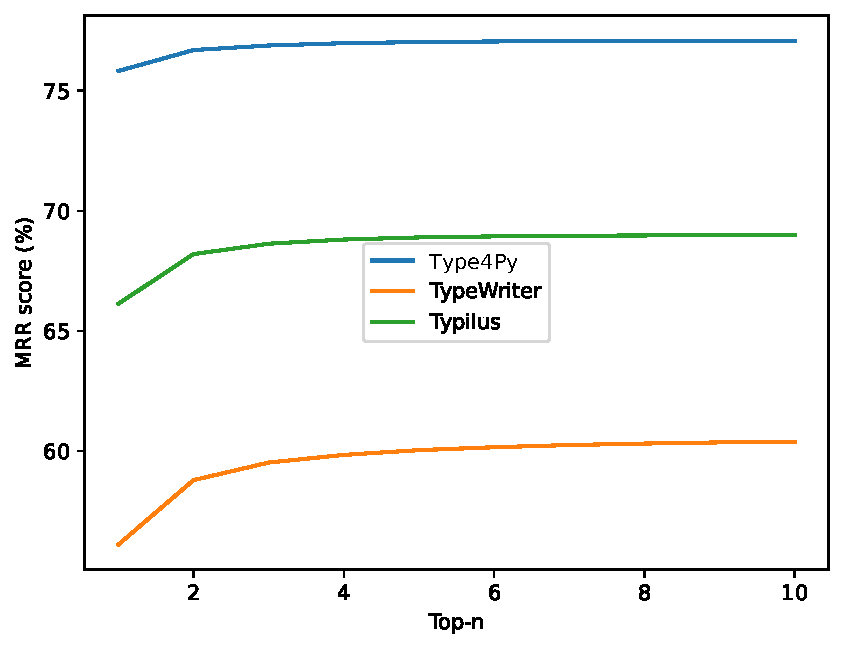
\includegraphics[width=0.75\linewidth]{chapters/ch4/figs/top-n-MRR.pdf}
	\caption{The MRR score of the models considering different top-$n$ predictions}
	\label{ch4:fig:top-n-MRR}
\end{figure}

As stated earlier, developers are more likely to use the first suggestion by a tool~\cite{parnin2011automated}. Therefore, we evaluated the neural models by the MRR@10 metric at the bottom of Table \ref{ch4:tab:top-n}. Ideally, the difference between the MRR@10 metric and the Top-1 prediction should be zero. However, this is very challenging as the neural models are not 100\% confident in their first suggestion for all test samples. Given the results of MRR@10, we observe that \name outperforms both Typilus and TypeWriter by a margin of 8.1\% and 16.7\%, respectively. In addition, we investigated the MRR score of the neural models while considering different values of Top-$n$, which is shown in Figure \ref{ch4:fig:top-n-MRR}. As can be seen, \name has a substantially higher score than the other models across all values of $n$. Moreover, the MRR score of all the three neural models almost converges to a fixed value after MRR@3. Given the findings of the RQ1, we use MRR@10 and the Top-1 prediction for the rest of the evaluation as we believe this better shows the practicality of the neural models for assisting developers.

\begin{table*}[!t]
	\centering
	\caption{Performance evaluation of the neural models considering different tasks}
	\label{ch4:tab:different-tasks}
	\begin{threeparttable}
		\resizebox{\textwidth}{!}{\begin{tabular}{@{}l l l c c c c c c c c c @{}}
			\toprule
			\multirow{2}{*}{Metric} & \multirow{2}{*}{Task} &  \multirow{2}{*}{Approach} & \multicolumn{4}{c}{\% Exact Match} & & \multicolumn{3}{c}{\% Base Type Match}& \\
			\cmidrule{4-7} \cmidrule{9-11}
			& & & All & Ubiquitous & Common & Rare & & All & Common & Rare & \\
			\midrule
			\multirow{10}{*}{Top-1 prediction} & \multirow{3}{*}{Argument} & \name & \textbf{61.9} & \textbf{100.0} & \textbf{64.5} & 17.4 & & \textbf{63.9} & \textbf{69.3} & 20.1 & \\
			& & Typilus  & 53.8 & 83.3 & 46.6 & \textbf{23.7} & & 57.0 & 52.5 & \textbf{29.6} & \\
			& & TypeWriter & 58.4 & 93.6 & 61.3 & 19.6 & & 60.1 & 64.4 & 22.1 & \\
			& & & & & & & & & & & \\
			& \multirow{3}{*}{Return}  & \name & \textbf{56.4} & \textbf{100.0} & 59.3 & \textbf{14.4} & & \textbf{60.3} & \textbf{65.4} & 20.9 & \\
			& & Typilus  & 42.5 & 84.0 & 41.6 & 12.3 & & 49.9 & 49.5 & \textbf{24.8} & \\
			& & TypeWriter  & 50.7 & 93.3 & \textbf{59.9} & 9.2 & & 54.1 & 64.4 & 15.0 & \\
			& & & & & & & & & & & \\
			& \multirow{2}{*}{Variable\tnote{a}}  & \name & \textbf{80.4} & \textbf{100.0} & \textbf{86.8} & 20.7 & & \textbf{85.9} & \textbf{89.1} & 44.6 & \\
			& & Typilus & 71.4 & 95.1 & 80.5 & \textbf{22.5} & & 80.7 & \textbf{89.1} & \textbf{48.6} & \\
			& & & & & & & & & & & \\
			\multirow{10}{*}{MRR@10} & \multirow{3}{*}{Argument} & \name & \textbf{64.2} & \textbf{100.0} & 69.5 & 20.7 & & \textbf{59.9} & 62.2 & 20.6 &  \\
			& & Typilus  & 58.7 & 87.9 & 55.4 & \textbf{27.5} & & 56.0 & 52.2 & \textbf{28.1} & \\
			& & TypeWriter & 63.3 & 96.2 & \textbf{72.4} & 23.0 & & 59.6 & \textbf{69.3} & 22.7 & \\
			& & & & & & & & & & &  \\
			& \multirow{3}{*}{Return}  & \name & \textbf{57.9} & \textbf{100.0} & 63.3 & \textbf{16.1} & & \textbf{52.9} & 55.8 & 18.5 & \\
			& & Typilus  & 46.0 & 86.9 & 49.8 & 14.3 & & 44.9 & 46.6 & \textbf{21.4} & \\
			& & TypeWriter  & 54.2 & 95.9 & \textbf{68.9} & 10.9 & & 49.9 & \textbf{65.1} & 14.2 & \\
			& & & & & & & & & & & \\
			& \multirow{2}{*}{Variable\tnote{a}}  & \name & \textbf{81.4} & \textbf{100.0} & \textbf{89.1} & 22.7 & & \textbf{79.1} & \textbf{85.0} & 34.1 & \\
			& & Typilus & 73.7 & 96.3 & 84.7 & \textbf{25.1} & & 72.4 & 82.7 & \textbf{36.1} & \\
			\bottomrule
		\end{tabular}}
		\begin{tablenotes}
			\item[a] {\footnotesize Note that TypeWriter cannot predict the type of variables.}
		\end{tablenotes}
	\end{threeparttable}
\end{table*}

\subsection{Different Prediction Tasks (\textbf{RQ}$_{2}$)}
Here, we compare \name with other baselines while considering different prediction tasks, i.e., arguments, return types, and variables.

\paragraph{Method}
Similar to the \RQ{1}, the models are trained and tested on the entire training and test sets, respectively.
However, we consider each prediction task separately while evaluating the models at Top-1 and MRR@10.

\paragraph{Results}
Table \ref{ch4:tab:different-tasks} shows the type prediction performance of the approaches for the three considered prediction tasks. In general, considering the exact match criteria (all), \name outperforms both Typilus and TypeWriter in all prediction tasks at both Top-1 and MRR@10. For instance, considering the return task and Top-1, \name obtains 56.4\% exact matches (all), which is 13.9\% and 5.7\% higher than that of Typilus and TypeWriter, respectively. Also, for the same task, the \name's MRR@10 is 11.9\% and 3.7\% higher compared to Typilus and TypeWriter, respectively. However, concerning the prediction of common types and MRR@10, TypeWriter performs better than both \name and Typilus at the argument and return tasks. This might be due to the fact that TypeWriter predicts from the set of 1,000 types, which apparently makes it better at the prediction of common types. Moreover, both \name and Typilus have a much larger type vocabulary and hence they need more training samples to generalize better providing that both argument and return types together amount to 22.8\% of all the data points in the dataset (see Table~\ref{ch4:tab:datapoints}). Lastly, in comparison with Typilus, \name obtains 7.7\% and 6.7\% higher MRR@10 score for the exact and base type match criteria (all), respectively.

\begin{table*}[!t]
	\centering
	\caption{Performance evaluation of \name with different configurations}
	\label{ch4:tab:models-different-configs}
	\resizebox{\textwidth}{!}{\begin{tabular}{@{}l l c c c c c c c c c @{}}
		\toprule
		\multirow{2}{*}{Metric} & \multirow{2}{*}{Approach} & \multicolumn{4}{c}{\% Exact Match} & & \multicolumn{3}{c}{\% Base Type Match\tnote{a}} & \\
		\cmidrule{3-6} \cmidrule{8-10}
		& & All & Ubiquitous & Common & Rare & & All & Common & Rare & \\
		\midrule
		\multirow{5}{*}{Top-1 prediction} & \name & \textbf{75.8} & \textbf{100.0} & 82.3 & \textbf{19.2} & & \textbf{80.6} & 85.2 & \textbf{36.0} & \\		
		& \name (w/o identifiers) & 72.7 & \textbf{100.0} & 71.8 & 17.4 & & 76.5 & 73.9 & 30.9 & \\
		& \name (w/o code context) & 67.9 & \textbf{100.0} & 59.2  & 11.4 & & 70.6 & 63.3 & 17.9 & \\
		& \name (w/o visible type hints)  & 65.4  & 86.2  & 71.9 & 15.8 & & 70.0 & 74.9 & 31.5 & \\
		& \name (w/ top 1,000 types)  & 74.5  & \textbf{100.0}  & \textbf{83.3} & 12.9 & & 79.1 & \textbf{86.3} & 28.5 & \\
		& & & & & & & & & & \\
		\multirow{5}{*}{MRR@10} & \name & \textbf{77.1} & \textbf{100.0} & 85.1  & \textbf{21.4} & & \textbf{74.1} & 79.9 & \textbf{29.4} & \\		
		& \name (w/o identifiers) & 73.8 & \textbf{100.0} & 74.6 & 19.2 & & 69.3 & 66.6 & 25.1 & \\
		& \name (w/o code context) & 69.7 & \textbf{100.0} & 63.9  & 13.6 & & 63.8 & 55.4 & 17.7 & \\
		& \name (w/o visible type hints) & 68.6  & 89.3 & 76.2 & 18.2 & & 65.8 & 70.1 & 26.2 & \\
		& \name (w/ top 1,000 types)  & 75.6  & \textbf{100.0}  & \textbf{86.2} & 14.2 & & 72.4 & \textbf{81.7} & 22.8 & \\
		\bottomrule
	\end{tabular}}
\end{table*}

\subsection{Ablation Analysis (\textbf{RQ}$_{3}$)}
\label{subsec:abalation}
Here, we investigate how each proposed type hint and the size of type vocabulary contribute to the overall performance of \name.

\paragraph{Method}
For ablation analysis, we trained and evaluated \name with 5 different configurations, i.e., (1) complete model (2) w/o identifiers (3) w/o code context (4) w/o visible type hints (5) w/ a vocabulary of top 1,000 types. Similar to the previous RQs, we measure the performance of \name with the described configurations at Top-1 and MRR@10.

\paragraph{Results}
Table \ref{ch4:tab:models-different-configs} presents the performance of \name with the five described configurations. It can be observed that all three type hints contribute significantly to the performance of \name. Code context has the most impact on the model's performance compared to the other two type hints. For instance, when ignoring code context, the model's exact match score for common types drops significantly by 23.1\%. After code context, visible type hints have a large impact on the performance of the model. By ignoring VTH, the model's exact match for ubiquitous types reduces from 100\% to 86.2\%. Although the Identifiers type hint contributes substantially to the prediction of common types, it has a less significant impact on the overall performance of \name compared to code context and VTH. In summary, we conclude that code context and VTH are the strongest type hints for our type prediction model.

By limiting the type vocabulary of \name to the top 1,000 types, similar to TypeWriter, we observe that the model's performance for common types is slightly improved while its performance for rare types is reduced significantly, i.e., 7.2\% considering MRR@10. This is expected as the model's type vocabulary is much smaller compared to the complete model's.

\begin{figure*}[!t]
	\centering
	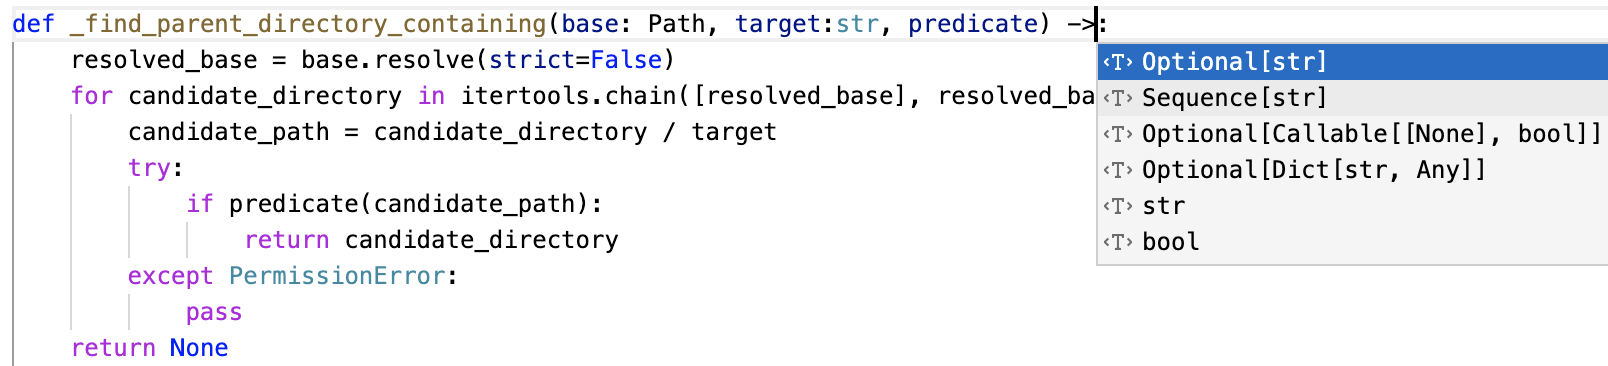
\includegraphics[width=\textwidth]{chapters/ch4/figs/VSC-IDE-pred.png}
	\caption{A type auto-completion example from VSC. The code has not been seen during training. The expected return type is \code{Optional[str]}.}
	\label{ch4:fig:VSC-IDE}
\end{figure*}

\section{Type4Py in Practice}\label{ch4:sec:prac}
To make the \name model practical, we developed an end-to-end solution including a web server and a Visual Studio Code (VSC) extension. We deployed this as an openly accessible web service that serves requests from the VSC extension. In this section, we describe the deployment components of \name.

\subsection{Deployment}
To deploy the pre-trained \name model for production, we convert the \name's PyTorch model to an ONNX model \cite{onnxruntime} which enables querying the model on both GPUs and CPUs with faster inference speed. Thanks to Annoy \cite{annoy}, a fast and memory-efficient KNN search is performed to suggest type annotations from type clusters.

\subsection{Web Server}
We have implemented a small Flask application to handle concurrent type prediction requests from users with Nginx as a proxy. This enables us to have quite a number of asynchronous workers that have an instance of \name’s ONNX model plus Type Clusters each. Specifically, the web application receives a Python source file via a POST request, queries an instance of the model, and finally it gives the file's predicted type annotations as a JSON response.

% TODO: Update No. of installation for the extension
\subsection{Visual Studio Code Extension}
As stated earlier, retrofitting type annotations is a daunting task for developers. To assist developers with this task, we have released a Visual Studio Code extension for \name~\cite{vscodet4py}, which uses the web server's API to provide ML-based type auto-completion for Python code. Figure \ref{ch4:fig:VSC-IDE} shows an example of a type recommendation from the VSC IDE. As of this writing, the extension has 909 installs on the Visual Studio Marketplace. Based on the user's consent, the VSC extension gathers telemetry data for research purposes. Specifically, accepted types, their rank in the list of suggestions, type slot kind, identifiers' name, and identifiers' line number are captured from the VSC environment and sent to our web server. In addition, rejected type predictions are captured when a type auto-completion window is closed without accepting a type.

By analyzing the gathered telemetry data from Jul. '21 to Aug. '21 and excluding the author(s), of 26 type auto-completion queries, 19 type annotations were accepted by the extension's users. Moreover, the average of accepted type annotations per developer is 69.6\%. Given that the gathered telemetry data is pretty small, we cannot draw a conclusion regarding the performance of \name in practice. However, our telemetry infrastructure and concerted efforts to broaden the user base will enable us to improve \name in the future.

\section{Discussion and Future Work}\label{ch4:sec:discuss}
Based on the formulated RQs and their evaluation in Section \ref{ch4:sec:eval}, we provide the following remarks:
\begin{itemize}
	%\setlength\itemsep{-0.2em}
	\item We used Pyre~\cite{pyre}, a static type inference tool, to augment our dataset with more type annotations. However, this can be considered as a \emph{weakly} supervision learning problem~\cite{zhou2018brief}, meaning that inferred types by the static tool might be noisy or imprecise despite the pre-processing steps. To eliminate this threat, we employed a static type checker, mypy, to remove source files with type errors from our dataset. Future work can devise a guided-search analysis to fix type errors in source files, which may improve the fix rate.
	
	\item It would be ideal for ML-based models to give a correct prediction in their first few suggestions, preferably Top-1, as developers tend to use the first suggestion by a tool~\cite{parnin2011automated}. Therefore, different from previous work on ML-based type prediction~\cite{pradel2019typewriter, allamanis2020typilus}, we use the MRR metric in our evaluation. We believe that the MRR metric better demonstrates the potential and usefulness of ML models to be used by developers in practice. Overall, considering the MRR metric, \name significantly outperforms the state-the-art ML-based type prediction models, namely, Typilus and TypeWriter.
	
	\item Considering the overall type prediction performance (\RQ{1}), both \name and Typilus generally perform better than TypeWriter. 
	This could be attributed to the fact that the two models map types into a
	high-dimensional space (i.e. type clusters). Hence this not only enables a much
	larger type vocabulary but also significantly improves their overall performance, especially the prediction
	of rare types.
	
	\item Given the results of \RQ{1} and \RQ{2}, our HNN-based neural model, \name, has empirically shown to be more effective than the GNN-based model of Typilus. We attribute this to the inherent bottleneck of GNNs which is over-squashing information into a fixed-size vector \cite{alon2020bottleneck} and thus they fail to capture long-range interaction. However, our HNN-based model concatenates learned features into a high-dimensional vector and hence it preserves information and its long-range dependencies.
	
	\item According to the results of ablation analysis (\RQ{3}), the three
	proposed type hints, i.e., identifiers, code context, and VTHs are
	all effective and positively contribute to the performance of \name. This result does not come
	at the expense of generalizability; our visible type analysis is not more
	sophisticated than what an IDE like PyCharm or VSCode do to determine
	available types for, e.g., auto-completion purposes.
	
	%	\item As indicated in the qualitative evaluation (\RQ{5}), the HNN-based model
	%    of \name has a better discriminative ability than the GNN-based model of Typilus, which results in a substantially higher type prediction performance. We attribute this to the inherent bottleneck of GNNs which is over-squashing information into a fixed-size vector \cite{alon2020bottleneck} and thus they fail to capture long-range interaction. However, our HNN-based model concatenates learned features into a high-dimensional vector and hence it preserves information and its long-range dependencies.
	
	\item Both \name and Typilus cannot make a correct prediction for types beyond their
	pre-defined (albeit very large) type clusters. For example, they currently cannot
	synthesize types, meaning that they will never suggest a type such as
	\texttt{Optional[Dict[str, int]]} if it does not exist in their type clusters.
	To address this, future research can explore pointer networks~\cite{vinyals2015pointer} or a GNN model that captures type system rules.
	
	\item We believe that \name's VSC extension is one step forward towards improving developers' productivity by using machine-aided code tools. 
	In this case, the VSC extension aids Python developers to retrofit types for their existing codebases. After gathering sufficiently large telemetry data from the usage of \name, we will study how to improve \name's ranking and quality of predictions for, ultimately, a better user experience.
\end{itemize}

\section{Summary}\label{ch4:sec:sum}
In this chapter, we present \name, a DSL-based hierarchical neural network type inference model for Python. It considers identifiers, code context, and visible type hints as features for learning to predict types. Specifically, the neural model learns to efficiently map types of the same kind into their own clusters in a high-dimensional space, and given type clusters, the $k$-nearest neighbor search is performed to infer the type of arguments, variables, and functions' return types. We used a type-checked dataset with sound type annotations to train and evaluate the ML-based type inference models. Overall, the results of our quantitative evaluation show that the \name model outperforms other state-of-the-art approaches. Most notably, considering the MRR@10 score, our proposed approach achieves a significantly higher score than that of Typilus and TypeWriter's by a margin of 8.1\% and 16.7\%, respectively. This indicates that our approach gives a more relevant prediction in its first suggestion, i.e., Top-1. Finally, we have deployed \name in an end-to-end fashion to provide ML-based type auto-completion in the VSC IDE and aid developers in retrofitting type annotations for their existing codebases.

\chapter{Conclusion}
\label{conclusion}
In the final chapter, we summarize this thesis's contributions, discuss the implications of the obtained results, and state possible research directions for future work.

\section{Revisiting Research Questions}
In this section, we reflect on the high-level research questions defined in the introduction and discuss the implications of the obtained results for the RQs.

\begin{description}
    \item[\RQ{1}] How effective is call graph pruning for security-focused applications?
\end{description}

The implications of both machine learning-based and non-learning-based call graph pruning techniques offer distinctive advantages and disadvantages, particularly in the context of security-focused applications. Each approach addresses different aspects of the requirements for practical static analysis, providing a multi-faceted perspective on enhancing the reliability and efficiency of security tools.

Machine learning-based call graph pruning, as demonstrated in Chapter~\ref{ch:effect_ml_cg_pruning}, can significantly improve the precision of static call graphs by approximately 25\%. This is a crucial refinement for reducing false positives and enhancing the reliability of downstream analyses. However, this method also introduces a trade-off with reduced recall or soundness, potentially leading to the omission of critical vulnerabilities due to pruned legitimate edges. Therefore, while ML-based pruning shows promise for speeding up security analyses through enhanced precision, it necessitates careful calibration of the balance between precision and recall, using the proposed conservative strategies, to avoid compromising soundness in vulnerability detection.

Conversely, the non-learning-based approach, exemplified by the \tool{OriginPruner} technique (presented in Chapter~\ref{ch:origin_pruner}), leverages domain knowledge and the origin methods to guide pruning decisions. This technique significantly reduces the size of call graphs without the need for extensive training data and at lower computational costs than ML-based methods. By focusing on the origin methods within the class hierarchy and localness analysis, \tool{OriginPruner} maintains the integrity of security analyses and ensures that no crucial edges are mistakenly omitted. This approach is particularly beneficial for security applications requiring rapid and accurate assessments, as it simplifies the call graphs while maintaining soundness, i.e., preserving the essential paths for vulnerability analysis.

The contrasting approaches highlight a different perspective to call graph pruning: the balance between using advanced machine learning techniques that require significant computational resources and training versus employing static, domain-knowledge-based methods that are less resource-intensive but might offer less flexibility in handling dynamic and complex software behaviors. Future research and practical applications in security-focused software analysis will likely benefit from a hybrid approach that combines the precision enhancement of ML-based pruning with the efficiency and reliability of non-learning-based methods. This combined approach could mitigate the limitations of each method and harness its strengths to improve the scalability and accuracy of security tools in real-world scenarios.

\begin{description}
\item[\RQ{2}] How does the call graph-based approach aid in reducing false positives in the vulnerability propagation analysis?
\end{description}

In Chapter~\ref{ch:effect_trans_gran}, we examined the effectiveness of a call graph-based approach in reducing false positives during vulnerability propagation analysis in software ecosystems, specifically within the Maven ecosystem. The study leverages empirical methods to demonstrate how incorporating a fine-grained analysis using call graphs significantly enhances the accuracy of identifying genuinely vulnerable packages by distinguishing between direct and transitive dependencies at different levels of granularity.

One key implication of the results is the substantial reduction in false positives when call graph-based analysis is applied. Traditional methods that evaluate vulnerability based on package dependencies alone tend to overestimate the security risks by marking the whole application with a vulnerable dependency as at risk. However, the findings show that only a few packages have executable paths that reach the vulnerable code within their dependencies. This distinction is critical because it implies that many software systems may not be as vulnerable as previously thought due to the lack of invocation of the insecure code. Thus, the call graph approach not only refines the accuracy of vulnerability assessments but also prioritizes allocating resources to mitigate critical security threats.

Moreover, the findings highlight the impact of granularity in the analysis of vulnerability propagation. By examining vulnerabilities at both the package and method levels, the study provides insights into how different levels of analysis can lead to vastly different results in the context of security risk assessment. For instance, while a package-level analysis identifies many potentially vulnerable packages, a method-level analysis using call graphs often reveals a much smaller subset where the vulnerable code is actively executed. This granular approach helps focus efforts on genuinely critical issues that require immediate attention, thus optimizing the effectiveness of security measures.

Another crucial aspect discussed in Chapter~\ref{ch:effect_trans_gran} is the concept of dependency depth. The study explores how limiting the depth of analysis to direct dependencies only (ignoring deeper transitive dependencies) can significantly reduce the computational burden of the analysis while still capturing a majority of the vulnerabilities that would actually impact the security of the application. This approach suggests a strategic compromise between depth of analysis and resource usage, which is particularly valuable for large-scale systems where extensive dependency chains are common.

In summary, Chapter~\ref{ch:effect_trans_gran} provides compelling evidence that call graph-based analysis is a more precise tool for vulnerability propagation analysis in software ecosystems. This method improves the accuracy of identifying vulnerable packages and helps efficiently prioritize security efforts. The insights from this study could guide future research and practices in software security, particularly in enhancing the tools and methodologies for vulnerability analysis in increasingly complex software environments.

\begin{description}
\item[\RQ{3}] How effective is machine learning in inferring type annotations for Python?
\end{description}

The results presented in Chapter~\ref{ch:t4py} highlight significant advancements in machine learning-based type inference for Python, showing a notable increase in Mean Reciprocal Rank over previous models like Typilus~\cite{allamanis2020typilus} and TypeWriter~\cite{pradel2019typewriter}. This improvement underscores the effectiveness of \tool{Type4Py}'s deep similarity learning approach, which better discriminates between similar and dissimilar types, thus enhancing the accuracy of type predictions. Using a type-checked dataset further adds to the robustness of the model, ensuring that the training and evaluation are based on sound type annotations, which mitigates the risk of learning from potentially incorrect data.

Given that \tool{Type4Py} achieves a higher MRR, particularly in its Top-1 suggestions, this suggests a significant step forward in practical usability. Developers are more likely to adopt a tool that consistently provides accurate suggestions at the top of its output list, as this reduces the effort required to select the correct type annotation manually. This feature directly translates into increased productivity and reduces the potential for errors in code, especially in dynamically typed languages like Python, where such errors are common.

Moreover, software maintainability can be significantly improved through accurate type inference. Type annotations make the code more understandable and easier to navigate, especially for new developers joining a project or revisiting old codebases. The ability of \tool{Type4Py} to retrofit accurate types into existing, untyped, or partially typed codebases can transform legacy Python code into more maintainable and modern code practices, aligning with Python's gradual typing philosophy introduced by PEP 484.

The ability of \tool{Type4Py} to provide highly accurate type suggestions indirectly affects developer productivity. Since the tool can reliably suggest the correct type annotation on the first try, developers spend less time typing and more time on actual problem-solving. This reduction in cognitive load can lead to faster development cycles, quicker feature rollouts, and more time allocated to optimizing code and implementing robust features. Furthermore, integrating such a tool within IDEs, as demonstrated by the Visual Studio Code extension, brings these benefits directly into the developer's environment, offering immediate and accessible benefits to their workflow.

Applying machine learning models like \tool{Type4Py} to infer type information pushes the boundary of what is possible with advanced programming practices in dynamically typed languages. It potentially opens the door to more sophisticated static analysis tools that were traditionally more effective in statically typed languages. For instance, more accurate type inference can enhance refactoring tools, code completion features, and sophisticated code analysis tools that can perform more in-depth checks and optimizations based on predicted types.

\section{Discussion}
In this section, based on the work presented in this thesis, we discuss 
the implications of the obtained results and research directions for future work.

\paragraph{Gathering high-quality data to train ML models is expensive} In Chapter~\ref{ch:effect_ml_cg_pruning} and Chapter~\ref{ch:t4py}, we applied deep learning techniques to tackle call graph pruning and type inference tasks, respectively. Our proposed model, \tool{Type4Py} outperformed state-of-the-art approaches at the time, namely, \tool{Typilus}~\cite{allamanis2020typilus} and \tool{TypeWriter}~\cite{pradel2019typewriter}. Despite the promising results, the proposed techniques must be trained or fine-tuned for the task at hand. Also, preparing ground truth is a daunting task per se, i.e., finding Python projects with sound type annotations or Java projects with high test coverage to build dynamic call graphs. Another alternative is to use heuristics and domain knowledge to solve the task, as shown in Chapter~\ref{ch:origin_pruner}. Very recently, (large) code language models have shown commendable performance in software engineering tasks due to their emergent capabilities, i.e., in-context learning~\cite{zheng2023survey}. Given this, using code language models might be a viable direction for future research in software analysis. Recent code language models, such as Codestral~\cite{codestral}, alleviate the need for data thanks to their zero-shot or few-short learning capabilities.

% \paragraph{Call graph pruning with the real-world vulnerabilities at the ecosystem level.} In Chapter~\ref{ch:effect_ml_cg_pruning} and Chapter~\ref{ch:origin_pruner}, we used artificial vulnerabilities to assess the effectiveness of (ML-based) call graph pruning techniques for the vulnerability analysis. To extend the obtained results in those two chapters, future work should investigate the efficacy of CG pruning techniques with real-world vulnerabilities at the ecosystem scale. Specifically, one can add a call graph pruner to our pipeline in Chapter~\ref{ch:effect_trans_gran} and then study its effect on the vulnerability propagation in the Maven ecosystem.

\paragraph{ML-based developer tools may not generalize beyond training data} In this thesis, we evaluated the trained or fine-tuned ML models on a set of unseen samples, namely, the test set, which is relatively small compared to the myriad of open-source software projects on the internet. Although their performance on the test sets was impressive, it is still unclear how an ML-based developer tool, \tool{Type4Py} would perform in real-world scenarios when used on different projects outside the ManyTypes4Py dataset. As described in Chapter~\ref{ch:t4py}, we gathered telemetry data when \tool{Type4Py} was used by developers in the Visual Studio Code extension. Similar to the studies done to evaluate code completion models in IDEs~\cite{izadi2024language, hellendoorn2019code}, future work can study to what extent developers accept the inferred type annotations by \tool{Type4Py} in the IDE. This also gives further insights into the real-world performance of \tool{Type4Py} and cases where it fails to infer a correct type annotation. Also, we generally recommend assessing the real-world performance of ML models trained for code-related tasks, as the ultimate goal is to boost developers' productivity by using these models.

\paragraph{A need for standard and systematic evaluation of ML-based developer tools} In addition to the real-world evaluation of the ML-based developers' tools, a micro-benchmark is needed to be developed that covers different language features. This is essential for assessing the performance of type inference and call graph pruning tools because it provides a controlled environment to measure and compare their effectiveness, providing modern applications that often leverage diverse language features~\cite{peng2021empirical}. In other words, micro-benchmarks can isolate specific language features, allowing for precise evaluation of how well these tools handle various constructs such as generics, lambdas, and reflection. This granularity helps identify inaccuracies in these tools, enabling researchers or practitioners to improve these tools systematically for better accuracy and completeness. Prasad et al.~\cite{venkatesh2023typeevalpy} proposed a micro-benchmark containing 845 test cases across 18 categories for the type inference task. A similar micro-benchmark should also be created to assess the effectiveness of call graph pruning techniques. For instance, one can start assessing the effect of CG pruning against the test suites proposed for CG soundness, known as the Judge benchmark~\cite{reif2019judge}.

\paragraph{Combination of machine learning and static analysis is promising} In this thesis, we showed that machine learning techniques can effectively be applied to tackle software analysis problems such as type inference and call graph pruning. However, recent work~\cite{peng2022static} has shown that a hybrid approach, i.e., the combination of machine learning and static analysis, is promising for inferring type annotation. Similarly, future work can investigate the efficacy of a hybrid call graph pruning approach, i.e., the combination of ML-based call graph pruners with \tool{OriginPruner}. Specifically, one can study how to use an ML-based CG pruner with \tool{OriginPruner} interchangeably or in combination to prune a CG edge.

\paragraph{Adoption of machine learning-based features into software analysis tools} In Chapter~\ref{ch:effect_ml_cg_pruning}, our empirical findings indicate that machine learning-based call graph pruning is an effective strategy for enhancing the precision of call graphs while maintaining their soundness, particularly in security-focused applications. However, similar to the previous work~\cite{le2022autopruner, utture2022striking}, our approach treats pruning as a subsequent step to constructing the call graph, which introduces a minor computational overhead. An alternative approach could involve embedding the ML-based pruning functionality directly within existing static analysis frameworks such as WALA~\cite{fink2012wala} and OPAL~\cite{eichberg2014software}. This feature enables users to prune edges or methods selectively during the call graph construction phase. This integration has the potential to yield more precise and compact call graphs and speed up the construction process. Aside from the pruning feature, one can achieve more accurate method resolution and variable interaction analysis by embedding a type inference component into the call graph construction tool for dynamic languages (e.g., Python). This, in turn, enhances the precision and soundness of the call graphs, making them more useful for tasks such as static code analysis, security vulnerability detection, and program understanding.

\paragraph{ML-based type inference for dynamic languages is still an open problem} 
In 2022, we published the \tool{Type4Py} technique, an ML-based type inference tool for Python. Following this, several research works have extended Type4Py or proposed other techniques to improve type inference for Python and other dynamic programming languages. These newer techniques include, but are not limited to, OppropBERT~\cite{jha2022oppropbert}, HiTyper~\cite{peng2022static}, TypeT5~\cite{wei2022typet5}, DiverseTyper~\cite{jesse2022learning}, Stir~\cite{peng2023statistical}, DeMinify~\cite{li2023deminify}, Tipical~\cite{elkobi2023tipical}, TypeGen~\cite{peng2023generative}, DeepInfer~\cite{zhao2023deepinfer}, PyAnalyzer~\cite{jin2024pyanalyzer}, and LExecutor~\cite{souza2023lexecutor}. Additionally, Type4Py was utilized as a type inference tool to address other intriguing research problems, such as docstring generation for Python~\cite{venkatkrishna2023docgen}, unit test generation~\cite{lukasczyk2022pynguin}, the development of fuzzing techniques~\cite{li2023pyrtfuzz}, and the study of dynamic typing-related practices in Python~\cite{chen2024risky}. Future work should look into local (small) large language models for type inference with retrieval augmented generation (RAG), which can be used inside IDEs. RAG might potentially help with user-defined type annotations in the project, which the LLM has not seen before.

\paragraph{Software ecosystem-level analysis is insightful but expensive to perform} We introduced the FASTEN project in Chapter~\ref{ch:intro}, which influenced how developers manage their projects' dependencies and assess the impact of security vulnerabilities on their projects. In short, In this thesis, we proposed a conservative ML-based call graph pruner and a non-learning-based approach (\tool{OriginPruner}). Since FASTEN operates at the ecosystem level, i.e., millions of projects and more than 10TB of data, these two CG pruning approaches can be a valuable extension to the FASTEN pipeline to make call graphs smaller and speed up vulnerability analysis. Also, this thesis investigated the vulnerability propagation in the Maven ecosystem from the perspective of transitivity and granularity. The obtained results in Chapter~\ref{ch:effect_trans_gran} empirically show the advantage of a fine-grained approach (i.e., call graph-level analysis) to the over-inflated dependency-level approach when analyzing security vulnerabilities in programs. In other words, we showed that FASTEN could be pretty helpful for developers in better assessing the risk of vulnerabilities found in their programs or dependencies used.  

\section{Summary}
% \subsection{Thesis contributions}
In this thesis, we showed that machine learning is promising for solving software analysis tasks like type inference and call graph pruning. Also, we investigated the effectiveness of dependency- and call graph-level vulnerability assessments in the Maven ecosystem. More specifically, this thesis makes the following contributions:

\begin{itemize}
    \item In this thesis, we introduced NYXCorpus, a benchmark dataset for evaluating machine learning-based call graph pruning techniques. By addressing limitations of the previous work, like imbalanced training data and reduced recall, we could implement conservative pruning strategies that improved the precision of call graphs while maintaining practicality for security applications. Our work also demonstrates that pruned call graphs retain high quality, comparable to context-sensitive analyses (1-CFA), but are produced faster and with smaller sizes (69\%), making downstream applications, i.e., vulnerability propagation, faster (up to 3.5 times).

    \item Given that ML models need high-quality data and have lofty inference cost, we developed \tool{OriginPruner}, a novel method leveraging method origin and localness analysis to prune false edges in static call graphs effectively. This approach not only reduces the size of the graphs but does so without compromising the soundness necessary for critical security applications, such as vulnerability propagation analysis. Our results confirm the effectiveness of incorporating domain-specific knowledge into pruning strategies, improving the precision of static program analysis with little computational overhead.

    \item Dependency-level analysis highly inflates the actual number of affected projects by security vulnerabilities. Motivated by this, this thesis investigated the impact of transitivity and granularity on vulnerability propagation through an empirical study in the Maven ecosystem. By shifting from dependency-level to method-level analysis, we provided a more accurate assessment of vulnerabilities, challenging the conventional overestimation of security risks in the previous work. Specifically, we found that less than 1\% of the packages have a reachable call path to vulnerable code in their dependencies. This fine-grained approach suggests a potential for significantly more efficient and accurate vulnerability assessments, which assists software developers in taking required actions to mitigate the vulnerability. 

    \item Retrofitting type annotations to existing codebases can be error-prone and laborious. To alleviate this, we proposed \tool{Type4Py}, a state-of-the-art ML-based type inference technique for Python, a dynamically typed language. By employing a deep similarity learning model, \tool{Type4Py} effectively distinguishes between type annotations in high-dimensional space, significantly improving the inference accuracy compared to the previous work. \tool{Type4Py} achieves an MRR of 77.1\%, which is a significant improvement of 8.1\% and 16.7\% over the state-of-the-art approaches Typilus and TypeWriter, respectively. Alongside its integration into a Visual Studio Code extension, \tool{Type4Py} aids developers by retrofitting type annotations into existing Python codebases, enhancing both productivity and code quality.
\end{itemize}

In conclusion, our research lays the foundation for a new era in software analysis, where machine learning and domain-specific knowledge converge to revolutionize how we develop and maintain software. Our novel and promising approaches not only push the boundaries of what is possible in software analysis but also pave the way for developing more accurate, scalable, and practical tools that will shape the future of software development. We hope this thesis's results inspire other researchers to explore ML-assisted software analysis and investigate how to seamlessly integrate it into developers' workflows, ultimately aiding them at various stages of the software development lifecycle.

%% Use letters for the chapter numbers of the appendices.
%\appendix

%\include{appendix-a/appendix-a}

%% Turn off thumb indices for unnumbered chapters.
\thumbfalse

\chapter*{Bibliography}
\addcontentsline{toc}{chapter}{Bibliography}
\setheader{Bibliography}

% URLs in this thesis have been archived on Archive.org. Their link target in digital editions refers
% to this timestamped version.

\bibliographystyle{unsrt}
% argument is your BibTeX string definitions and bibliography database(s)
\bibliography{dissertation}

%% \chapter*{Glossary}
% \glsaddall
% \printglossary[type=\acronymtype,title={Glossary}]
% \addcontentsline{toc}{chapter}{Glossary}
% \setheader{Glossary}

\chapter*{Curriculum Vit\ae}
\addcontentsline{toc}{chapter}{Curriculum Vit\ae}
\setheader{Curriculum Vit\ae}

%% Print the full name of the author.
\makeatletter
\authors{\@firstname\ {\titleshape\@lastname}}
\makeatother

\noindent
\begin{longtable}{p{.225\textwidth} p{.70\textwidth}}
    1993/04/07 & Date of birth in Tehran, Iran
\end{longtable}

\section*{Education}
\begin{longtable}{p{.225\textwidth} p{.70\textwidth}}
    10/2019-06/2024 & Ph.D. Student, Software Engineering Research Group (SERG), \\
     & Delft University of Technology, The Netherlands, \\
     & Thesis: Machine Learning-assisted Software Analysis, A \\
     & Supervisors: Dr. Sebastian Proksch (2021-2024) \\
     &  \hspace*{5.1em} Dr. Georgios Gousios (2019-2020) \\
     & Promotor: Prof. Dr. Arie van Deursen \\
     & \\

     01/2016-01/2019 & M.Sc., Computer Engineering (Artificial Intelligence), \\
     & Azad University (North Tehran Branch), Tehran, Iran, \\
     & Thesis: Robust Twin Support Vector Machine for Noisy Data, 4/4 \\
     & Supervisor: Dr. Jalal A. Nasiri \\
     & \\

     10/2011-07/2015 & B.Sc., Computer, University of Tehran, Tehran, Iran \\
     & Thesis: Applications of the Python Programming Language for Climatology, 3.95/4\\
     & \\
     07/2010-07/2011 & Pre-university Diploma, Alavi, Tehran, Iran \\
     10/2007-06/2010 & High School Diploma, Andisheh, Tehran, Iran \\    
\end{longtable}

\section*{Experience}
\begin{longtable}{p{.225\textwidth} p{.70\textwidth}}
    10/2019-09/2022 & Research Software Engineer, the FASTEN Project, \\
    & Delft University of Technology, The Netherlands \\
    & \\
    07/2017-09/2019 &  Research Assistant, Machine Learning and Text Mining Lab \\
    & Iranian Research Institute for Information Science (IranDoc), Tehran, Iran \\
\end{longtable}

\newpage
\section*{Academic Service}
\begin{longtable}{p{.225\textwidth} p{.70\textwidth}}
    Chair & Social Media and Publicity Co-chair MSR 2024 \\
    & \\
    PC Member &  ASE, Industry Track, 2024 \\
    & ICSE 2024, Artifact Evaluation \\
    & NLBSE 2024 \\
    & MSR 2023 (Junior PC) \\
    & \\

    Reviewer & ICLR 2023 \\
             & JSS 2023 \\
             & TOSEM 2023 \\
             & Expert Systems with Applications, 2021\\
             & FSE 2021, Artifact Evaluation (external) \\
             & \\
    
    Council Member & PhD council of the Institute for Programming \\
                  &  Research and Algorithmics (IPA), 2021-2024 \\
                  & \\

    Student Volunteer & ICSE 2024 \\
    & \\

    Virtualization (Live Stream) & ICSE 2020 \\
    & \\
    Co-supervision & Lang Feng's Master Thesis "Static Analysis Complements Machine Learning: A Type Inference Use Case", 2022-2023 \\
    & Jonathan Katzy's Master Thesis "Utilizing Lingual Structures to Enhance Transformer Performance in Source Code Completions", 2021-2022 \\
    & Bachelor end project of a group of three students studying the combination of static analysis with deep learning to improve type inference for Python, 2022 \\
    & \\
    Teaching Assistant & Release Engineering for Machine Learning, Dr. S. Proksch \& Dr. L. Cruz, 2022 \\
    & Machine Learning for Software Engineering, Dr. Georgios Gousios, 2020 \\ 
\end{longtable}


\chapter*{List of Publications}
\addcontentsline{toc}{chapter}{List of Publications}
\setheader{List of Publications}
\label{publications}

%% We use the 'etaremune' environment (the reverse of 'enumerate') to get a
%% numbered list of publications in reverse chronological order. If the list of
%% authors is long, it might be useful to emphasize your own name with \textbf.
\begin{etaremune}{\small
\item[\faFileTextO~~1.] \textbf{Amir M. Mir}, Mehdi Keshani, and Sebastian Proksch. On the Effectiveness of Machine Learning-based Call Graph Pruning: An Empirical Study. In IEEE/ACM 21st International Conference on Mining
Software Repositories (MSR'24), April 2024

\item[\faFileTextO~~2.] \textbf{Amir M. Mir}, Mehdi Keshani, and Sebastian Proksch. On the Effect of Transitivity and Granularity on Vulnerability Propagation in the Maven Ecosystem. In Proceedings of the 30th IEEE International
Conference on Software Analysis, Evolution and Reengineering (SANER'23), March 2023

\item[\faFileTextO~~3.] \textbf{Amir M. Mir}, Evaldas Latoskinas, Sebastian Proksch, and Georgios Gousios. Type4Py: Practical Deep Similarity Learning-based Type Inference for Python. In Proceedings of the 44th International Conference on
Software Engineering (ICSE'22), pages 2241–2252, May 2022

\item[\faFileTextO~~4.] \textbf{Amir M. Mir}, Evaldas Latoskinas, and Georgios Gousios. ManyTypes4Py: A Benchmark Python Dataset for
Machine Learning-Based Type Inference. In IEEE/ACM 18th International Conference on Mining Software Repositories (MSR'21), pages 585–589, May 2021

\item[5.] Venkatesh, A. P. S., Sabu, S., Wang, J., \textbf{Mir, A. M.}, Li, L., \& Bodden, E. TypeEvalPy: A Micro-benchmarking Framework for Python Type Inference Tools. Tool Demonstration, In Proceedings of 46th International Conference on Software Engineering (ICSE'24), April 2024

\item[6.] Venkatesh, A. P. S., Sabu, S., \textbf{Mir, A. M.}, Reis, S., \& Bodden, E. (2024). The Emergence of Large Language Models in Static Analysis: A First Look through Micro-Benchmarks. First special event of AI Foundation Models and Software Engineering (FORGE'24), April 2024
}
\end{etaremune}

\vspace{0.5cm}
\noindent
\faFileTextO~~Included in this thesis.\\
% \faTrophy~~Won a best paper, tool demonstration, or proposal award.

%%%%%%%%%%%%%%%%%%%%%%%%%%%%%%%%%%%%%%%%%%%%%%%%%%%%%%%%%%%%%%%%%%%%%%
%%%%%%%
%
% IPA Dissertation Series.
%
% (c) Jan Joris Vereijken <janjoris@acm.org>
%
% Time-stamp: <Mon Oct 13 13:32:28 MET DST 1997, snd.2941
%janjoris@wsinfm14>
%
%
% Modified by Pedro R. D'Argenio <dargenio@cs.utwente.nl>
%         and Judi Romijn <judi@cs.kun.nl>
%
% Time-stamp: <Wed Sep  1 13:09:47 MET DST 1999>
%
% Package 'multicol' required.
%


\newcommand*{\promitem}[4]{\noindent \textbf{#1}. \emph{#2}. #3.~\mbox{#4}\medskip}

\clearpage \pagestyle{empty}

%\footnotesize
\setlength{\columnsep}{2em}
\begin{multicols}{2}
        [\subsection*{Titles in the IPA Dissertation Series since 2022}]




%\promitem{J.O. Blanco}
%         {The State Operator in Process Algebra}
%         {Faculty of Mathematics and Computing Science, TUE}
%        {1996-01}

%\promitem{A.M. Geerling}
%         {Transformational Development of Data-Parallel Algorithms}
%         {Faculty of Mathematics and Computer Science, KUN}
%         {1996-02}

%\promitem{P.M. Achten}
%         {Interactive Functional Programs: Models, Methods, and
%          Implementation}
%         {Faculty of Mathematics and Computer Science, KUN}
%         {1996-03}

%\promitem{M.G.A. Verhoeven}
%         {Parallel Local Search}
%         {Faculty of Mathematics and Computing Science, TUE}
%         {1996-04}

%\promitem{M.H.G.K. Kesseler}
%         {The Implementation of Functional Languages on Parallel
%          Machines with Distrib.\ Memory}
%         {Faculty of Mathematics and Computer Science, KUN}
%         {1996-05}

%\promitem{D. Alstein}
%         {Distributed Algorithms for Hard Real-Time Systems}
%         {Faculty of Mathematics and Computing Science, TUE}
%         {1996-06}

%\promitem{J.H. Hoepman}
%         {Communication, Synchronization, and Fault-Tolerance}
%         {Faculty of Mathematics and Computer Science, UvA}
%         {1996-07}

%\promitem{H. Doornbos}
%         {Reductivity Arguments and Program Construction}
%         {Faculty of Mathematics and Computing Science, TUE}
%         {1996-08}

%\promitem{D. Turi}
%         {Functorial Operational Semantics and its Denotational Dual}
%         {Faculty of Mathematics and Computer Science, VUA}
%         {1996-09}

%\promitem{A.M.G. Peeters}
%         {Single-Rail Handshake Circuits}
%         {Faculty of Mathematics and Computing Science, TUE}
%         {1996-10}

%\promitem{N.W.A. Arends}
%         {A Systems Engineering Specification Formalism}
%         {Faculty of Mechanical Engineering, TUE}
%         {1996-11}

%\promitem{P. Severi de Santiago}
%         {Normalisation in Lambda Calculus and its Relation to Type
%          Inference}
%         {Faculty of Mathematics and Computing Science, TUE}
%         {1996-12}

%\promitem{D.R. Dams}
%         {Abstract Interpretation and Partition Refinement for Model
%          Checking}
%         {Faculty of Mathematics and Computing Science, TUE}
%         {1996-13}

%\promitem{M.M. Bonsangue}
%         {Topological Dualities in Semantics}
%         {Faculty of Mathematics and Computer Science, VUA}
%         {1996-14}

%\promitem{B.L.E. de Fluiter}
%         {Algorithms for Graphs of Small Treewidth}
%         {Faculty of Mathematics and Computer Science, UU}
%         {1997-01}

%\promitem{W.T.M. Kars}
%         {Process-algebraic Transformations in Context}
%         {Faculty of Computer Science, UT}
%         {1997-02}

%\promitem{P.F. Hoogendijk}
%         {A Generic Theory of Data Types}
%         {Faculty of Mathematics and Computing Science, TUE}
%         {1997-03}

%\promitem{T.D.L. Laan}
%         {The Evolution of Type Theory in Logic and Mathematics}
%         {Faculty of Mathematics and Computing Science, TUE}
%         {1997-04}

%\promitem{C.J. Bloo}
%         {Preservation of Termination for Explicit Substitution}
%         {Faculty of Mathematics and Computing Science, TUE}
%        {1997-05}

%\promitem{J.J. Vereijken}
%         {Discrete-Time Process Algebra}
%         {Faculty of Mathematics and Computing Science, TUE}
%         {1997-06}

%\promitem{F.A.M. van den Beuken}
%         {A Functional Approach to Syntax and Typing}
%         {Faculty of Mathematics and Informatics, KUN}
%         {1997-07}

%\promitem{A.W. Heerink}
%         {Ins and Outs in Refusal Testing}
%         {Faculty of Computer Science, UT}
%         {1998-01}

%\promitem{G. Naumoski and W. Alberts}
%         {A Discrete-Event Simulator for Systems Engineering}
%         {Faculty of Mechanical Engineering, TUE}
%         {1998-02}

%\promitem{J. Verriet}
%         {Scheduling with Communication for Multiprocessor
%          Computation}
%         {Faculty of Mathematics and Computer Science, UU}
%         {1998-03}

%\promitem{J.S.H. van Gageldonk}
%         {An Asynchronous Low-Power 80C51 Microcontroller}
%         {Faculty of Mathematics and Computing Science, TUE}
%         {1998-04}

%\promitem{A.A. Basten}
%         {In Terms of Nets: System Design with Petri Nets and Process
%          Algebra}
%         {Faculty of Mathematics and Computing Science, TUE}
%         {1998-05}

%\promitem{E. Voermans}
%         {Inductive Datatypes with Laws and Subtyping -- A Relational
%          Model}
%         {Faculty of Mathematics and Computing Science, TUE}
%         {1999-01}

%\promitem{H. ter Doest}
%         {Towards Probabilistic Unification-based Parsing}
%         {Faculty of Computer Science, UT}
%         {1999-02}

%\promitem{J.P.L. Segers}
%         {Algorithms for the Simulation of Surface Processes}
%         {Faculty of Mathematics and Computing Science, TUE}
%         {1999-03}

%\promitem{C.H.M. van Kemenade}
%         {Recombinative Evolutionary Search}
%         {Faculty of Mathematics and Natural Sciences, UL}
%         {1999-04}

%\promitem{E.I. Barakova}
%         {Learning Reliability: a Study on Indecisiveness in Sample
%          Selection}
%         {Faculty of Mathematics and Natural Sciences, RUG}
%         {1999-05}

%\promitem{M.P. Bodlaender}
%         {Scheduler Optimization in Real-Time Distributed Databases}
%         {Faculty of Mathematics and Computing Science, TUE}
%         {1999-06}

%\promitem{M.A. Reniers}
%         {Message Sequence Chart: Syntax and Semantics}
%         {Faculty of Mathematics and Computing Science, TUE}
%         {1999-07}

%\promitem{J.P. Warners}
%         {Nonlinear approaches to satisfiability problems}
%         {Faculty of Mathematics and Computing Science, TUE}
%         {1999-08}

%\promitem{J.M.T. Romijn}
%         {Analysing Industrial Protocols with Formal Methods}
%         {Faculty of Computer Science, UT}
%         {1999-09}

%\promitem{P.R. D'Argenio}
%         {Algebras and Automata for Timed and Stochastic Systems}
%         {Faculty of Computer Science, UT}
%         {1999-10}

%\promitem{G. F\'abi\'an}
%         {A Language and Simulator for Hybrid Systems}
%         {Faculty of Mechanical Engineering, TUE}
%         {1999-11}

%\promitem{J. Zwanenburg}
%         {Object-Oriented Concepts and Proof Rules}
%         {Faculty of Mathematics and Computing Science, TUE}
%         {1999-12}

%\promitem{R.S. Venema}
%         {Aspects of an Integrated Neural Prediction System}
%         {Faculty of Mathematics and Natural Sciences, RUG}
%         {1999-13}

%\promitem{J. Saraiva}
%         {A Purely Functional Implementation of Attribute Grammars}
%         {Faculty of Mathematics and Computer Science, UU}
%         {1999-14}

%\promitem{R. Schiefer}
%         {Viper, A Visualisation Tool for Parallel Program
%          Construction}
%         {Faculty of Mathematics and Computing Science, TUE}
%         {1999-15}

%\promitem{K.M.M. de Leeuw}
%         {Cryptology and Statecraft in the Dutch Republic}
%         {Faculty of Mathematics and Computer Science, UvA}
%         {2000-01}

%\promitem{T.E.J. Vos}
%         {UNITY in Diversity. A stratified approach to the
%          verification of distributed algorithms}
%         {Faculty of Mathematics and Computer Science, UU}
%         {2000-02}

%\promitem{W. Mallon}
%         {Theories and Tools for the Design of Delay-Insensitive
%          Communicating Processes}
%         {Faculty of Mathematics and Natural Sciences, RUG}
%         {2000-03}

%\promitem{W.O.D. Griffioen}
%         {Studies in Computer Aided Verification of Protocols}
%         {Faculty of Science, KUN}
%         {2000-04}

%\promitem{P.H.F.M. Verhoeven}
%         {The Design of the MathSpad Editor}
%         {Faculty of Mathematics and Computing Science, TUE}
%         {2000-05}

%\promitem{J. Fey}
%         {Design of a Fruit Juice Blending and Packaging Plant}
%         {Faculty of Mechanical Engineering, TUE}
%         {2000-06}

%\promitem{M. Franssen}
%         {Cocktail: A Tool for Deriving Correct Programs}
%         {Faculty of Mathematics and Computing Science, TUE}
%         {2000-07}

%\promitem{P.A. Olivier}
%         {A Framework for Debugging Heterogeneous Applications}
%         {Faculty of Natural Sciences, Mathematics and Computer
%          Science, UvA}
%         {2000-08}

%\promitem{E. Saaman}
%        {Another Formal Specification Language}
%         {Faculty of Mathematics and Natural Sciences, RUG}
%         {2000-10}

%\promitem{M. Jelasity}
%         {The Shape of Evolutionary Search Discovering and
%          Representing Search Space Structure}
%         {Faculty of Mathematics and Natural Sciences, UL}
%         {2001-01}

%\promitem{R. Ahn}
%         {Agents, Objects and Events a computational approach to knowledge, observation and
%          communication}
%         {Faculty of Mathematics and Computing Science, TU/e}
%         {2001-02}%

%\promitem{M. Huisman}
%         {Reasoning about Java programs in higher order logic using PVS
%          and Isabelle}
%         {Faculty of Science, KUN}
%         {2001-03}

%\promitem{I.M.M.J. Reymen}
%         {Improving Design Processes through Structured Reflection}
%         {Faculty of Mathematics and Computing Science, TU/e}
%         {2001-04}

%\promitem{S.C.C. Blom}
%         {Term Graph Rewriting: syntax and semantics}
%         {Faculty of Sciences, Division of Mathematics and Computer Science,
%          VUA}
%         {2001-05}

%\promitem{R. van Liere}
%         {Studies in Interactive Visualization}
%         {Faculty of Natural Sciences, Mathematics and Computer
%          Science, UvA}
%         {2001-06}

%\promitem{A.G. Engels}
%         {Languages for Analysis and Testing of Event Sequences}
%         {Faculty of Mathematics and Computing Science, TU/e}
%         {2001-07}

%\promitem{J. Hage}
%         {Structural Aspects of Switching Classes}
%         {Faculty of Mathematics and Natural Sciences, UL}
%         {2001-08}

%\promitem{M.H. Lamers}
%         {Neural Networks for Analysis of Data in Environmental
%          Epidemiology: A Case-study into Acute Effects of Air Pollution Episodes}
%         {Faculty of Mathematics and Natural Sciences, UL}
%         {2001-09}

%\promitem{T.C. Ruys}
%         {Towards Effective Model Checking}
%         {Faculty of Computer Science, UT}
%         {2001-10}

%\promitem{D. Chkliaev}
%         {Mechanical verification of concurrency control and recovery protocols}
%         {Faculty of Mathematics and Computing Science, TU/e}
%         {2001-11}

%\promitem{M.D. Oostdijk}
%         {Generation and presentation of formal mathematical documents}
%         {Faculty of Mathematics and Computing Science, TU/e}
%         {2001-12}

%\promitem{A.T. Hofkamp}
%         {Reactive machine control: A simulation approach using $\chi$}
%         {Faculty of Mechanical Engineering, TU/e}
%         {2001-13}

%\promitem{D. Bo\v{s}na\v{c}ki}
%         {Enhancing state space reduction techniques for model checking}
%         {Faculty of Mathematics and Computing Science, TU/e}
%         {2001-14}
%
%\promitem{M.C. van Wezel}
%         {Neural Networks for Intelligent Data Analysis: theoretical and
%         experimental aspects}
%         {Faculty of Mathematics and Natural Sciences, UL}
%         {2002-01}
%
%\promitem{V. Bos and J.J.T. Kleijn}
%         {Formal Specification and Analysis of Industrial Systems}
%         {Faculty of Mathematics and Computer Science and Faculty of Mechanical Engineering, TU/e}
%         {2002-02}
%
%\promitem{T. Kuipers}
%         {Techniques for Understanding Legacy Software Systems}
%         {Faculty of Natural Sciences, Mathematics and Computer
%          Science, UvA}
%         {2002-03}
%
%\promitem{S.P. Luttik}
%         {Choice Quantification in Process Algebra}
%         {Faculty of Natural Sciences, Mathematics, and Computer Science, UvA}
%         {2002-04}
%
%\promitem{R.J. Willemen}
%         {School Timetable Construction: Algorithms and Complexity}
%         {Faculty of Mathematics and Computer Science, TU/e}
%         {2002-05}
%
%\promitem{M.I.A. Stoelinga}
%         {Alea Jacta Est: Verification of Probabilistic, Real-time and Parametric Systems}
%         {Faculty of Science, Mathematics and Computer Science, KUN}
%         {2002-06}
%
%\promitem{N. van Vugt}
%         {Models of Molecular Computing}
%         {Faculty of Mathematics and Natural Sciences, UL}
%         {2002-07}
%
%\promitem{A. Fehnker}
%         {Citius, Vilius, Melius: Guiding and Cost-Optimality in Model Checking of Timed and Hybrid Systems}
%         {Faculty of Science, Mathematics and Computer Science, KUN}
%         {2002-08}
%
%\promitem{R. van Stee}
%         {On-line Scheduling and Bin Packing}
%         {Faculty of Mathematics and Natural Sciences, UL}
%         {2002-09}
%
%\promitem{D. Tauritz}
%         {Adaptive Information Filtering: Concepts and Algorithms}
%         {Faculty of Mathematics and Natural Sciences, UL}
%         {2002-10}
%
%\promitem{M.B. van der Zwaag}
%         {Models and Logics for Process Algebra}
%         {Faculty of Natural Sciences, Mathematics, and Computer
%          Science, UvA}
%         {2002-11}
%
%\promitem{J.I. den Hartog}
%         {Probabilistic Extensions of Semantical Models}
%         {Faculty of Sciences, Division of Mathematics and Computer Science, VUA}
%         {2002-12}
%
%\promitem{L. Moonen}
%         {Exploring Software Systems}
%         {Faculty of Natural Sciences, Mathematics, and Computer
%          Science, UvA}
%         {2002-13}
%
%\promitem{J.I. van Hemert}
%         {Applying Evolutionary Computation to Constraint Satisfaction and
%          Data Mining}
%         {Faculty of Mathematics and Natural Sciences, UL}
%         {2002-14}
%
%\promitem{S. Andova}
%         {Probabilistic Process Algebra}
%         {Faculty of Mathematics and Computer Science, TU/e}
%         {2002-15}
%
%\promitem{Y.S. Usenko}
%         {Linearization in $\mu$CRL}
%         {Faculty of Mathematics and Computer Science, TU/e}
%         {2002-16}
%
%\promitem{J.J.D. Aerts}
%         {Random Redundant Storage for Video on Demand}
%         {Faculty of Mathematics and Computer Science, TU/e}
%         {2003-01}
%
%\promitem{M. de Jonge}
%         {To Reuse or To Be Reused: Techniques for component composition and construction}
%         {Faculty of Natural Sciences, Mathematics, and Computer
%          Science, UvA}
%         {2003-02}
%
%\promitem{J.M.W. Visser}
%         {Generic Traversal over Typed Source Code Representations}
%         {Faculty of Natural Sciences, Mathematics, and Computer
%          Science, UvA}
%         {2003-03}
%
%\promitem{S.M. Bohte}
%         {Spiking Neural Networks}
%         {Faculty of Mathematics and Natural Sciences, UL}
%         {2003-04}
%
%\promitem{T.A.C. Willemse}
%         {Semantics and Verification in Process Algebras with Data and Timing}
%         {Faculty of Mathematics and Computer Science, TU/e}
%         {2003-05}
%
%\promitem{S.V. Nedea}
%         {Analysis and Simulations of Catalytic Reactions}
%         {Faculty of Mathematics and Computer Science, TU/e}
%         {2003-06}
%
%\promitem{M.E.M. Lijding}
%         {Real-time Scheduling of Tertiary Storage}
%         {Faculty of Electrical Engineering, Mathematics \& Computer Science, UT}
%         {2003-07}
%
%\promitem{H.P. Benz}
%         {Casual Multimedia Process Annotation -- CoMPAs}
%         {Faculty of Electrical Engineering, Mathematics \& Computer Science, UT}
%         {2003-08}
%
%\promitem{D. Distefano}
%         {On Modelchecking the Dynamics of Object-based Software: a Foundational
%          Approach}
%         {Faculty of Electrical Engineering, Mathematics \& Computer Science, UT}
%         {2003-09}
%
%\promitem{M.H. ter Beek}
%         {Team Automata -- A Formal Approach to the Modeling of Collaboration Between System Components}
%         {Faculty of Mathematics and Natural Sciences, UL}
%         {2003-10}
%
%\promitem{D.J.P. Leijen}
%         {The $\lambda$ Abroad -- A Functional Approach to Software Components}
%         {Faculty of Mathematics and Computer Science, UU}
%         {2003-11}
%
%\promitem{W.P.A.J. Michiels}
%         {Performance Ratios for the Differencing Method}
%         {Faculty of Mathematics and Computer Science, TU/e}
%         {2004-01}
%
%\promitem{G.I. Jojgov}
%         {Incomplete Proofs and Terms and Their Use in Interactive Theorem Proving}
%         {Faculty of Mathematics and Computer Science, TU/e}
%         {2004-02}
%
%\promitem{P. Frisco}
%         {Theory of Molecular Computing -- Splicing and Membrane systems}
%         {Faculty of Mathematics and Natural Sciences, UL}
%         {2004-03}
%
%\promitem{S. Maneth}
%         {Models of Tree Translation}
%         {Faculty of Mathematics and Natural Sciences, UL}
%         {2004-04}
%
%\promitem{Y. Qian}
%         {Data Synchronization and Browsing for Home Environments}
%         {Faculty of Mathematics and Computer Science and Faculty of Industrial Design, TU/e}
%         {2004-05}
%
%\promitem{F. Bartels}
%         {On Generalised Coinduction and Probabilistic Specification Formats}
%         {Faculty of Sciences, Division of Mathematics and Computer Science, VUA}
%         {2004-06}
%
%\promitem{L. Cruz-Filipe}
%         {Constructive Real Analysis: a Type-Theoretical Formalization and Applications}
%         {Faculty of Science, Mathematics and Computer Science, KUN}
%         {2004-07}
%
%\promitem{E.H. Gerding}
%         {Autonomous Agents in Bargaining Games: An Evolutionary Investigation of Fundamentals, Strategies, and Business Applications}
%         {Faculty of Technology Management, TU/e}
%         {2004-08}
%
%\promitem{N. Goga}
%         {Control and Selection Techniques for the Automated Testing of Reactive Systems}
%         {Faculty of Mathematics and Computer Science, TU/e}
%         {2004-09}
%
%\promitem{M. Niqui}
%         {Formalising Exact Arithmetic: Representations, Algorithms and Proofs}
%         {Faculty of Science, Mathematics and Computer Science, RU}
%         {2004-10}
%
%\promitem{A. L\"{o}h}
%         {Exploring Generic Haskell}
%         {Faculty of Mathematics and Computer Science, UU}
%         {2004-11}
%
%\promitem{I.C.M. Flinsenberg}
%         {Route Planning Algorithms for Car Navigation}
%         {Faculty of Mathematics and Computer Science, TU/e}
%         {2004-12}
%
%\promitem{R.J. Bril}
%         {Real-time Scheduling for Media Processing Using Conditionally Guaranteed Budgets}
%         {Faculty of Mathematics and Computer Science, TU/e}
%         {2004-13}
%
%\promitem{J. Pang}
%         {Formal Verification of Distributed Systems}
%         {Faculty of Sciences, Division of Mathematics and Computer Science, VUA}
%         {2004-14}
%
%\promitem{F. Alkemade}
%         {Evolutionary Agent-Based Economics}
%         {Faculty of Technology Management, TU/e}
%         {2004-15}
%
%\promitem{E.O. Dijk}
%         {Indoor Ultrasonic Position Estimation Using a Single Base Station}
%         {Faculty of Mathematics and Computer Science, TU/e}
%         {2004-16}
%
%
%\promitem{S.M. Orzan}
%         {On Distributed Verification and Verified Distribution}
%         {Faculty of Sciences, Division of Mathematics and Computer Science, VUA}
%         {2004-17}
%
%\promitem{M.M. Schrage}
%         {Proxima - A Presentation-oriented Editor for Structured Documents}
%         {Faculty of Mathematics and Computer Science, UU}
%         {2004-18}
%
%\promitem{E. Eskenazi and A. Fyukov}
%         {Quantitative Prediction of Quality Attributes for Component-Based Software Architectures}
%         {Faculty of Mathematics and Computer Science, TU/e}
%         {2004-19}
%
%\promitem{P.J.L. Cuijpers}
%         {Hybrid Process Algebra}
%         {Faculty of Mathematics and Computer Science, TU/e}
%         {2004-20}
%
%\promitem{N.J.M. van den Nieuwelaar}
%         {Supervisory Machine Control by Predictive-Reactive Scheduling}
%         {Faculty of Mechanical Engineering, TU/e}
%         {2004-21}
%
%\promitem{E. \'{A}brah\'{a}m}
%         {An Assertional Proof System for Multithreaded Java -Theory and Tool Support- }
%         {Faculty of Mathematics and Natural Sciences, UL}
%         {2005-01}
%
%\promitem{R. Ruimerman}
%         {Modeling and Remodeling in Bone Tissue}
%         {Faculty of Biomedical Engineering, TU/e}
%         {2005-02}
%
%\promitem{C.N. Chong}
%         {Experiments in Rights Control - Expression and Enforcement}
%         {Faculty of Electrical Engineering, Mathematics \& Computer Science, UT}
%         {2005-03}
%
%\promitem{H. Gao}
%         {Design and Verification of Lock-free Parallel Algorithms}
%         {Faculty of Mathematics and Computing Sciences, RUG}
%         {2005-04}
%
%\promitem{H.M.A. van Beek}
%         {Specification and Analysis of Internet Applications}
%         {Faculty of Mathematics and Computer Science, TU/e}
%         {2005-05}
%
%\promitem{M.T. Ionita}
%         {Scenario-Based System Architecting - A Systematic Approach to Developing Future-Proof System Architectures}
%         {Faculty of Mathematics and Computing Sciences, TU/e}
%         {2005-06}
%
%\promitem{G. Lenzini}
%         {Integration of Analysis Techniques in Security and Fault-Tolerance}
%         {Faculty of Electrical Engineering, Mathematics \& Computer Science, UT}
%         {2005-07}
%
%\promitem{I. Kurtev}
%         {Adaptability of Model Transformations}
%         {Faculty of Electrical Engineering, Mathematics \& Computer Science, UT}
%         {2005-08}
%
%\promitem{T. Wolle}
%         {Computational Aspects of Treewidth - Lower Bounds and Network Reliability}
%         {Faculty of Science, UU}
%         {2005-09}
%
%\promitem{O. Tveretina}
%         {Decision Procedures for Equality Logic with Uninterpreted Functions}
%         {Faculty of Mathematics and Computer Science, TU/e}
%         {2005-10}
%
%\promitem{A.M.L. Liekens}
%         {Evolution of Finite Populations in Dynamic Environments}
%         {Faculty of Biomedical Engineering, TU/e}
%         {2005-11}
%
%\promitem{J. Eggermont}
%         {Data Mining using Genetic Programming: Classification and Symbolic Regression}
%         {Faculty of Mathematics and Natural Sciences, UL}
%         {2005-12}
%
%\promitem{B.J. Heeren}
%         {Top Quality Type Error Messages}
%         {Faculty of Science, UU}
%         {2005-13}
%
%\promitem{G.F. Frehse}
%         {Compositional Verification of Hybrid Systems using Simulation Relations}
%         {Faculty of Science, Mathematics and Computer Science, RU}
%         {2005-14}
%
%\promitem{M.R. Mousavi}
%         {Structuring Structural Operational Semantics}
%         {Faculty of Mathematics and Computer Science, TU/e}
%         {2005-15}
%
%\promitem{A. Sokolova}
%         {Coalgebraic Analysis of Probabilistic Systems}
%         {Faculty of Mathematics and Computer Science, TU/e}
%         {2005-16}
%
%\promitem{T. Gelsema}
%         {Effective Models for the Structure of pi-Calculus Processes with Replication}
%         {Faculty of Mathematics and Natural Sciences, UL}
%         {2005-17}
%
%\promitem{P. Zoeteweij}
%         {Composing Constraint Solvers}
%         {Faculty of Natural Sciences, Mathematics, and Computer Science, UvA}
%         {2005-18}
%
%\promitem{J.J. Vinju}
%         {Analysis and Transformation of Source Code by Parsing and Rewriting}
%         {Faculty of Natural Sciences, Mathematics, and Computer Science, UvA}
%         {2005-19}
%
%\promitem{M.Valero Espada}
%         {Modal Abstraction and Replication of Processes with Data}
%         {Faculty of Sciences, Division of Mathematics and Computer Science, VUA}
%         {2005-20}
%
%\promitem{A. Dijkstra}
%         {Stepping through Haskell}
%         {Faculty of Science, UU}
%         {2005-21}
%
%\promitem{Y.W. Law}
%         {Key management and link-layer security of wireless sensor networks: energy-efficient attack and defense}
%         {Faculty of Electrical Engineering, Mathematics \& Computer Science, UT}
%         {2005-22}
%
%\promitem{E. Dolstra}
%         {The Purely Functional Software Deployment Model}
%         {Faculty of Science, UU}
%         {2006-01}
%
%\promitem{R.J. Corin}
%         {Analysis Models for Security Protocols}
%         {Faculty of Electrical Engineering, Mathematics \& Computer Science, UT}
%         {2006-02}
%
%\promitem{P.R.A. Verbaan}
%         {The Computational Complexity of Evolving Systems}
%         {Faculty of Science, UU}
%         {2006-03}
%
%\promitem{K.L. Man and R.R.H. Schiffelers}
%         {Formal Specification and Analysis of Hybrid Systems}
%         {Faculty of Mathematics and Computer Science and Faculty of Mechanical Engineering, TU/e}
%         {2006-04}
%
%\promitem{M. Kyas}
%         {Verifying OCL Specifications of UML Models: Tool Support and Compositionality}
%         {Faculty of Mathematics and Natural Sciences, UL}
%         {2006-05}
%
%\promitem{M. Hendriks}
%         {Model Checking Timed Automata - Techniques and Applications}
%         {Faculty of Science, Mathematics and Computer Science, RU}
%         {2006-06}
%
%\promitem{J. Ketema}
%         {B\"ohm-Like Trees for Rewriting}
%         {Faculty of Sciences, VUA}
%         {2006-07}
%
%\promitem{C.-B. Breunesse}
%         {On JML: topics in tool-assisted verification of JML programs}
%         {Faculty of Science, Mathematics and Computer Science, RU}
%         {2006-08}
%
%\promitem{B. Markvoort}
%         {Towards Hybrid Molecular Simulations}
%         {Faculty of Biomedical Engineering, TU/e}
%         {2006-09}
%
%\promitem{S.G.R. Nijssen}
%         {Mining Structured Data}
%         {Faculty of Mathematics and Natural Sciences, UL}
%         {2006-10}
%
%\promitem{G. Russello}
%         {Separation and Adaptation of Concerns in a Shared Data Space}
%         {Faculty of Mathematics and Computer Science, TU/e}
%         {2006-11}
%
%\promitem{L. Cheung}
%         {Reconciling Nondeterministic and Probabilistic Choices}
%         {Faculty of Science, Mathematics and Computer Science, RU}
%         {2006-12}
%
%\promitem{B. Badban}
%         {Verification techniques for Extensions of Equality Logic}
%         {Faculty of Sciences, Division of Mathematics and Computer Science, VUA}
%         {2006-13}
%
%\promitem{A.J. Mooij}
%         {Constructive formal methods and protocol standardization}
%         {Faculty of Mathematics and Computer Science, TU/e}
%         {2006-14}
%
%\promitem{T. Krilavicius}
%         {Hybrid Techniques for Hybrid Systems}
%         {Faculty of Electrical Engineering, Mathematics \& Computer Science, UT}
%         {2006-15}
%
%\promitem{M.E. Warnier}
%         {Language Based Security for Java and JML}
%         {Faculty of Science, Mathematics and Computer Science, RU}
%         {2006-16}
%
%\promitem{V. Sundramoorthy}
%         {At Home In Service Discovery}
%         {Faculty of Electrical Engineering, Mathematics \& Computer Science, UT}
%         {2006-17}
%
%\promitem{B. Gebremichael}
%         {Expressivity of Timed Automata Models}
%         {Faculty of Science, Mathematics and Computer Science, RU}
%         {2006-18}
%
%\promitem{L.C.M. van Gool}
%         {Formalising Interface Specifications}
%         {Faculty of Mathematics and Computer Science, TU/e}
%         {2006-19}
%
%\promitem{C.J.F. Cremers}
%         {Scyther - Semantics and Verification of Security Protocols}
%         {Faculty of Mathematics and Computer Science, TU/e}
%         {2006-20}
%
%\promitem{J.V. Guillen Scholten}
%         {Mobile Channels for Exogenous Coordination of Distributed Systems: Semantics, Implementation and Composition}
%         {Faculty of Mathematics and Natural Sciences, UL}
%         {2006-21}
%
%\promitem{H.A. de Jong}
%         {Flexible Heterogeneous Software Systems}
%         {Faculty of Natural Sciences, Mathematics, and Computer Science, UvA}
%         {2007-01}
%
%\promitem{N.K. Kavaldjiev}
%         {A run-time reconfigurable Network-on-Chip for streaming DSP applications}
%         {Faculty of Electrical Engineering, Mathematics \& Computer Science, UT}
%         {2007-02}
%
%
%\promitem{M. van Veelen}
%         {Considerations on Modeling for Early Detection of Abnormalities in Locally Autonomous Distributed Systems}
%         {Faculty of Mathematics and Computing Sciences, RUG}
%         {2007-03}
%
%\promitem{T.D. Vu}
%         {Semantics and Applications of Process and Program Algebra}
%         {Faculty of Natural Sciences, Mathematics, and Computer Science, UvA}
%         {2007-04}
%
%\promitem{L. Brand\'an Briones}
%         {Theories for Model-based Testing: Real-time and Coverage}
%         {Faculty of Electrical Engineering, Mathematics \& Computer Science, UT}
%         {2007-05}
%
%\promitem{I. Loeb}
%         {Natural Deduction: Sharing by Presentation}
%         {Faculty of Science, Mathematics and Computer Science, RU}
%         {2007-06}
%
%\promitem{M.W.A. Streppel}
%         {Multifunctional Geometric Data Structures}
%         {Faculty of Mathematics and Computer Science, TU/e}
%         {2007-07}
%
%\promitem{N. Tr\v{c}ka}
%         {Silent Steps in Transition Systems and Markov Chains}
%         {Faculty of Mathematics and Computer Science, TU/e}
%         {2007-08}
%
%\promitem{R. Brinkman}
%         {Searching in encrypted data}
%         {Faculty of Electrical Engineering, Mathematics \& Computer Science, UT}
%         {2007-09}
%
%\promitem{A. van Weelden}
%         {Putting types to good use}
%         {Faculty of Science, Mathematics and Computer Science, RU}
%         {2007-10}
%
%\promitem{J.A.R. Noppen}
%         {Imperfect Information in Software Development Processes}
%         {Faculty of Electrical Engineering, Mathematics \& Computer Science, UT}
%         {2007-11}
%
%\promitem{R. Boumen}
%         {Integration and Test plans for Complex Manufacturing Systems}
%         {Faculty of Mechanical Engineering, TU/e}
%         {2007-12}
%
%\promitem{A.J. Wijs}
%         {What to do Next?: Analysing and Optimising System Behaviour in Time}
%         {Faculty of Sciences, Division of Mathematics and Computer Science, VUA}
%         {2007-13}
%
%\promitem{C.F.J. Lange}
%         {Assessing and Improving the Quality of Modeling: A Series of Empirical Studies about the UML}
%         {Faculty of Mathematics and Computer Science, TU/e}
%         {2007-14}
%
%
%\promitem{T. van der Storm}
%         {Component-based Configuration, Integration and Delivery}
%         {Faculty of Natural Sciences, Mathematics, and Computer Science,UvA}
%         {2007-15}
%
%
%\promitem{B.S. Graaf}
%         {Model-Driven Evolution of Software Architectures}
%         {Faculty of Electrical Engineering, Mathematics, and Computer Science, TUD}
%         {2007-16}
%
%\promitem{A.H.J. Mathijssen}
%         {Logical Calculi for Reasoning with Binding}
%         {Faculty of Mathematics and Computer Science, TU/e}
%         {2007-17}
%
%\promitem{D. Jarnikov}
%         {QoS framework for Video Streaming in Home Networks}
%         {Faculty of Mathematics and Computer Science, TU/e}
%         {2007-18}
%
%\promitem{M. A. Abam}
%         {New Data Structures and Algorithms for Mobile Data}
%         {Faculty of Mathematics and Computer Science, TU/e}
%         {2007-19}
%
%
%\promitem{W. Pieters}
%         {La Volont\'{e} Machinale: Understanding the Electronic Voting Controversy}
%         {Faculty of Science, Mathematics and Computer Science, RU}
%         {2008-01}
%
%\promitem{A.L. de Groot}
%         {Practical Automaton Proofs in PVS}
%         {Faculty of Science, Mathematics and Computer Science, RU}
%         {2008-02}
%
%\promitem{M. Bruntink}
%         {Renovation of Idiomatic Crosscutting Concerns in Embedded Systems}
%         {Faculty of Electrical Engineering, Mathematics, and Computer Science, TUD}
%         {2008-03}
%
%\promitem{A.M. Marin}
%         {An Integrated System to Manage Crosscutting Concerns in Source Code}
%         {Faculty of Electrical Engineering, Mathematics, and Computer Science, TUD}
%         {2008-04}
%
%\promitem{N.C.W.M. Braspenning}
%         {Model-based Integration and Testing of High-tech Multi-disciplinary Systems}
%         {Faculty of Mechanical Engineering, TU/e}
%         {2008-05}
%
%\promitem{M. Bravenboer}
%         {Exercises in Free Syntax: Syntax Definition, Parsing, and Assimilation of Language Conglomerates}
%         {Faculty of Science, UU}
%         {2008-06}
%
%\promitem{M. Torabi Dashti}
%         {Keeping Fairness Alive: Design and Formal Verification of Optimistic Fair Exchange Protocols}
%         {Faculty of Sciences, Division of Mathematics and Computer Science, VUA}
%         {2008-07}
%
%\promitem{I.S.M. de Jong}
%         {Integration and Test Strategies for Complex Manufacturing Machines}
%         {Faculty of Mechanical Engineering, TU/e}
%         {2008-08}
%
%\promitem{I. Hasuo}
%         {Tracing Anonymity with Coalgebras}
%         {Faculty of Science, Mathematics and Computer Science, RU}
%         {2008-09}
%
%\promitem{L.G.W.A. Cleophas}
%         {Tree Algorithms: Two Taxonomies and a Toolkit}
%         {Faculty of Mathematics and Computer Science, TU/e}
%         {2008-10}
%
%\promitem{I.S. Zapreev}
%         {Model Checking Markov Chains: Techniques and Tools}
%         {Faculty of Electrical Engineering, Mathematics \& Computer Science, UT}
%         {2008-11}
%
%\promitem{M. Farshi}
%         {A Theoretical and Experimental Study of Geometric Networks}
%     {Faculty of Mathematics and Computer Science, TU/e}
%         {2008-12}
%
%\promitem{G. Gulesir}
%         {Evolvable Behavior Specifications Using Context-Sensitive Wildcards}
%         {Faculty of Electrical Engineering, Mathematics \& Computer Science, UT}
%         {2008-13}
%
%\promitem{F.D. Garcia}
%         {Formal and Computational Cryptography: Protocols, Hashes and Commitments}
%     {Faculty of Science, Mathematics and Computer Science, RU}
%         {2008-14}
%
%\promitem{P. E. A. D\"{u}rr}
%         {Resource-based Verification for Robust Composition of Aspects}
%         {Faculty of Electrical Engineering, Mathematics \& Computer Science, UT}
%         {2008-15}
%
%\promitem{E.M. Bortnik}
%         {Formal Methods in Support of SMC Design}
%         {Faculty of Mechanical Engineering, TU/e}
%         {2008-16}
%
%\promitem{R.H. Mak}
%         {Design and Performance Analysis of Data-Independent Stream Processing       Systems}
%         {Faculty of Mathematics and Computer Science, TU/e}
%         {2008-17}
%
%\promitem{M. van der Horst}
%         {Scalable Block Processing Algorithms}
%         {Faculty of Mathematics and Computer Science, TU/e}
%         {2008-18}
%
%\promitem{C.M. Gray}
%         {Algorithms for Fat Objects: Decompositions and Applications}
%         {Faculty of Mathematics and Computer Science, TU/e}
%         {2008-19}
%
%\promitem{J.R. Calam\'{e}}
%         {Testing Reactive Systems with Data - Enumerative Methods and Constraint Solving}
%         {Faculty of Electrical Engineering, Mathematics \& Computer Science, UT}
%         {2008-20}
%
%\promitem{E. Mumford}
%         {Drawing Graphs for Cartographic Applications}
%         {Faculty of Mathematics and Computer Science, TU/e}
%         {2008-21}
%
%\promitem{E.H. de Graaf}
%         {Mining Semi-structured Data, Theoretical and Experimental Aspects of Pattern Evaluation}
%         {Faculty of Mathematics and Natural Sciences, UL}
%         {2008-22}
%
%\promitem{R. Brijder}
%         {Models of Natural Computation: Gene Assembly and Membrane Systems}
%         {Faculty of Mathematics and Natural Sciences, UL}
%         {2008-23}
%
%\promitem{A. Koprowski}
%         {Termination of Rewriting and Its Certification}
%         {Faculty of Mathematics and Computer Science, TU/e}
%         {2008-24}
%
%\promitem{U. Khadim}
%         {Process Algebras for Hybrid Systems: Comparison and Development}
%         {Faculty of Mathematics and Computer Science, TU/e}
%         {2008-25}
%
%\promitem{J. Markovski}
%         {Real and Stochastic Time in Process Algebras for Performance Evaluation}
%         {Faculty of Mathematics and Computer Science, TU/e}
%         {2008-26}
%
%
%\promitem{H. Kastenberg}
%         {Graph-Based Software Specification and Verification}
%         {Faculty of Electrical Engineering, Mathematics \& Computer Science, UT}
%         {2008-27}
%
%\promitem{I.R. Buhan}
%         {Cryptographic Keys from Noisy Data Theory and Applications}
%         {Faculty of Electrical Engineering, Mathematics \& Computer Science, UT}
%         {2008-28}
%
%\promitem{R.S. Marin-Perianu}
%         {Wireless Sensor Networks in Motion: Clustering Algorithms for Service Discovery and Provisioning}
%         {Faculty of Electrical Engineering, Mathematics \& Computer Science, UT}
%         {2008-29}
%
%
%\promitem{M.H.G. Verhoef}
%         {Modeling and Validating Distributed Embedded Real-Time Control Systems}
%         {Faculty of Science, Mathematics and Computer Science, RU}
%         {2009-01}
%
%\promitem{M. de Mol}
%         {Reasoning about Functional Programs: Sparkle, a proof assistant for Clean}
%         {Faculty of Science, Mathematics and Computer Science, RU}
%         {2009-02}
%
%\promitem{M. Lormans}
%         {Managing Requirements Evolution}
%         {Faculty of Electrical Engineering, Mathematics, and Computer Science, TUD}
%         {2009-03}
%
%\promitem{M.P.W.J. van Osch}
%         {Automated Model-based Testing of Hybrid Systems}
%         {Faculty of Mathematics and Computer Science, TU/e}
%         {2009-04}
%
%\promitem{H. Sozer}
%         {Architecting Fault-Tolerant Software Systems}
%         {Faculty of Electrical Engineering, Mathematics \& Computer Science, UT}
%         {2009-05}
%
%\promitem{M.J. van Weerdenburg}
%         {Efficient Rewriting Techniques}
%         {Faculty of Mathematics and Computer Science, TU/e}
%         {2009-06}
%
%\promitem{H.H. Hansen}
%         {Coalgebraic Modelling: Applications in Automata Theory and Modal Logic}
%         {Faculty of Sciences, Division of Mathematics and Computer Science, VUA}
%         {2009-07}
%
%\promitem{A. Mesbah}
%         {Analysis and Testing of Ajax-based Single-page Web Applications}
%         {Faculty of Electrical Engineering, Mathematics, and Computer Science, TUD}
%         {2009-08}
%
%\promitem{A.L. Rodriguez Yakushev}
%         {Towards Getting Generic Programming Ready for Prime Time}
%         {Faculty of Science, UU}
%         {2009-9}
%
%\promitem{K.R. Olmos Joffr\'e}
%         {Strategies for Context Sensitive Program Transformation}
%         {Faculty of Science, UU}
%         {2009-10}
%
%\promitem{J.A.G.M. van den Berg}
%         {Reasoning about Java programs in PVS using JML}
%         {Faculty of Science, Mathematics and Computer Science, RU}
%         {2009-11}
%
%\promitem{M.G. Khatib}
%         {MEMS-Based Storage Devices. Integration in Energy-Constrained Mobile Systems}
%         {Faculty of Electrical Engineering, Mathematics \& Computer Science, UT}
%         {2009-12}
%
%\promitem{S.G.M. Cornelissen}
%         {Evaluating Dynamic Analysis Techniques for Program Comprehension}
%         {Faculty of Electrical Engineering, Mathematics, and Computer Science, TUD}
%         {2009-13}
%
%\promitem{D. Bolzoni}
%         {Revisiting Anomaly-based Network Intrusion Detection Systems}
%         {Faculty of Electrical Engineering, Mathematics \& Computer Science, UT}
%         {2009-14}
%
%\promitem{H.L. Jonker}
%         {Security Matters: Privacy in Voting and Fairness in Digital Exchange}
%         {Faculty of Mathematics and Computer Science, TU/e}
%         {2009-15}
%
%\promitem{M.R. Czenko}
%         {TuLiP - Reshaping Trust Management}
%         {Faculty of Electrical Engineering, Mathematics \& Computer Science, UT}
%         {2009-16}
%
%\promitem{T. Chen}
%         {Clocks, Dice and Processes}
%         {Faculty of Sciences, Division of Mathematics and Computer Science, VUA}
%         {2009-17}
%
%\promitem{C. Kaliszyk}
%         {Correctness and Availability:
% Building Computer Algebra on top of Proof Assistants and making Proof
%Assistants available over the Web}
%         {Faculty of Science, Mathematics and Computer Science, RU}
%         {2009-18}
%
%\promitem{R.S.S. O'Connor}
%         {Incompleteness \& Completeness: Formalizing Logic and Analysis in Type Theory}
%         {Faculty of Science, Mathematics and Computer Science, RU}
%         {2009-19}
%
%\promitem{B. Ploeger}
%         {Improved Verification Methods for Concurrent Systems}
%         {Faculty of Mathematics and Computer Science, TU/e}
%         {2009-20}
%
%\promitem{T. Han}
%         {Diagnosis, Synthesis and Analysis of Probabilistic Models}
%         {Faculty of Electrical Engineering, Mathematics \& Computer Science, UT}
%         {2009-21}
%
%\promitem{R. Li}
%         {Mixed-Integer Evolution Strategies for Parameter Optimization and Their Applications to Medical Image Analysis}
%         {Faculty of Mathematics and Natural Sciences, UL}
%         {2009-22}
%
%\promitem{J.H.P. Kwisthout}
%         {The Computational Complexity of Probabilistic Networks}
%         {Faculty of Science, UU}
%         {2009-23}
%
%\promitem{T.K. Cocx}
%         {Algorithmic Tools for Data-Oriented Law Enforcement}
%         {Faculty of Mathematics and Natural Sciences, UL}
%         {2009-24}
%
%\promitem{A.I. Baars}
%         {Embedded Compilers}
%         {Faculty of Science, UU}
%         {2009-25}
%
%\promitem{M.A.C. Dekker}
%         {Flexible Access Control for Dynamic Collaborative Environments}
%         {Faculty of Electrical Engineering, Mathematics \& Computer Science, UT}
%         {2009-26}
%
%\promitem{J.F.J. Laros}
%         {Metrics and Visualisation for Crime Analysis and Genomics}
%         {Faculty of Mathematics and Natural Sciences, UL}
%         {2009-27}
%
%\promitem{C.J. Boogerd}
%         {Focusing Automatic Code Inspections}
%         {Faculty of Electrical Engineering, Mathematics, and Computer Science, TUD}
%         {2010-01}
%
%\promitem{M.R. Neuh\"au{\ss}er}
%         {Model Checking Nondeterministic and Randomly Timed Systems}
%         {Faculty of Electrical Engineering, Mathematics \& Computer Science, UT}
%         {2010-02}
%
%\promitem{J. Endrullis}
%         {Termination and Productivity}
%         {Faculty of Sciences, Division of Mathematics and Computer Science, VUA}
%         {2010-03}
%
%\promitem{T. Staijen}
%         {Graph-Based Specification and Verification for Aspect-Oriented Languages}
%         {Faculty of Electrical Engineering, Mathematics \& Computer Science, UT}
%         {2010-04}
%
%\promitem{Y.  Wang}
%         {Epistemic Modelling and Protocol Dynamics}
%         {Faculty of Science, UvA}
%         {2010-05}
%
%\promitem{J.K.  Berendsen}
%         {Abstraction, Prices and Probability in Model Checking Timed Automata}
%         {Faculty of Science, Mathematics and Computer Science, RU}
%         {2010-06}
%
%\promitem{A. Nugroho}
%         {The Effects of UML Modeling on the Quality of Software}
%         {Faculty of Mathematics and Natural Sciences, UL}
%         {2010-07}
%
%\promitem{A. Silva}
%         {Kleene Coalgebra}
%         {Faculty of Science, Mathematics and Computer Science, RU}
%         {2010-08}
%
%\promitem{J.S. de Bruin}
%         {Service-Oriented Discovery of Knowledge - Foundations, Implementations and Applications}
%         {Faculty of Mathematics and Natural Sciences, UL}
%         {2010-09}
%
%\promitem{D. Costa}
%         {Formal Models for Component Connectors}
%         {Faculty of Sciences, Division of Mathematics and Computer Science, VUA}
%         {2010-10}
%
%\promitem{M.M. Jaghoori}
%         {Time at Your Service: Schedulability Analysis of Real-Time and Distributed Services}
%         {Faculty of Mathematics and Natural Sciences, UL}
%         {2010-11}
%
%\promitem{R. Bakhshi}
%         {Gossiping Models: Formal Analysis of Epidemic Protocols}
%         {Faculty of Sciences, Department of Computer Science, VUA}
%         {2011-01}
%
%\promitem{B.J. Arnoldus}
%         {An Illumination of the Template Enigma: Software Code Generation with Templates}
%         {Faculty of Mathematics and Computer Science, TU/e}
%         {2011-02}
%
%\promitem{E. Zambon}
%         {Towards Optimal IT Availability Planning: Methods and Tools}
%         {Faculty of Electrical Engineering, Mathematics \& Computer Science, UT}
%         {2011-03}
%
%\promitem{L. Astefanoaei}
%         {An Executable Theory of Multi-Agent Systems Refinement}
%         {Faculty of Mathematics and Natural Sciences, UL}
%         {2011-04}
%
%\promitem{J. Proen{\c c}a}
%         {Synchronous coordination of distributed components}
%         {Faculty of Mathematics and Natural Sciences, UL}
%         {2011-05}
%
%\promitem{A. Moral\i}
%         {IT Architecture-Based Confidentiality Risk Assessment in Networks of Organizations}
%         {Faculty of Electrical Engineering, Mathematics \& Computer Science, UT}
%         {2011-06}
%
%\promitem{M. van der Bijl}
%         {On changing models in Model-Based Testing}
%         {Faculty of Electrical Engineering, Mathematics \& Computer Science, UT}
%         {2011-07}
%
%\promitem{C. Krause}
%         {Reconfigurable Component Connectors}
%         {Faculty of Mathematics and Natural Sciences, UL}
%         {2011-08}
%
%\promitem{M.E. Andr\'es}
%         {Quantitative Analysis of Information Leakage in Probabilistic and Nondeterministic Systems}
%         {Faculty of Science, Mathematics and Computer Science, RU}
%         {2011-09}
%
%\promitem{M. Atif}
%         {Formal Modeling and Verification of Distributed Failure Detectors}
%         {Faculty of Mathematics and Computer Science, TU/e}
%         {2011-10}
%
%\promitem{P.J.A. van Tilburg}
%         {From Computability to Executability -- A process-theoretic view on automata theory}
%         {Faculty of Mathematics and Computer Science, TU/e}
%         {2011-11}
%         
%\promitem{Z. Protic}
%         {Configuration management for models: Generic methods for model comparison and model co-evolution}
%         {Faculty of Mathematics and Computer Science, TU/e}
%         {2011-12}
% 
%\promitem{S. Georgievska}
%         {Probability and Hiding in Concurrent Processes}
%         {Faculty of Mathematics and Computer Science, TU/e}
%         {2011-13}
%
%\promitem{S. Malakuti}
%         {Event Composition Model: Achieving Naturalness in Runtime Enforcement}
%         {Faculty of Electrical Engineering, Mathematics \& Computer Science, UT}
%         {2011-14}
%
%\promitem{M. Raffelsieper}
%         {Cell Libraries and Verification}
%         {Faculty of Mathematics and Computer Science, TU/e}
%         {2011-15}
%
%\promitem{C.P. Tsirogiannis}
%         {Analysis of Flow and Visibility on Triangulated Terrains}
%         {Faculty of Mathematics and Computer Science, TU/e}
%         {2011-16}
%
%\promitem{Y.-J. Moon}
%         {Stochastic Models for Quality of Service of Component Connectors}
%         {Faculty of Mathematics and Natural Sciences, UL}
%         {2011-17}
%
%\promitem{R. Middelkoop}
%         {Capturing and Exploiting Abstract Views of States in OO Verification}
%         {Faculty of Mathematics and Computer Science, TU/e}
%         {2011-18}
%
%\promitem{M.F. van Amstel}
%         {Assessing and Improving the Quality of Model Transformations}
%         {Faculty of Mathematics and Computer Science, TU/e}
%         {2011-19}
%
%\promitem{A.N. Tamalet}
%         {Towards Correct Programs in Practice}
%         {Faculty of Science, Mathematics and Computer Science, RU}
%         {2011-20}
%
%\promitem{H.J.S. Basten}
%         {Ambiguity Detection for Programming Language Grammars}
%         {Faculty of Science, UvA}
%         {2011-21}
%
%\promitem{M. Izadi}
%         {Model Checking of Component Connectors}
%         {Faculty of Mathematics and Natural Sciences, UL}
%         {2011-22}
%
%\promitem{L.C.L. Kats}
%         {Building Blocks for Language Workbenches}
%         {Faculty of Electrical Engineering, Mathematics, and Computer Science, TUD}
%         {2011-23}
%
%\promitem{S. Kemper}
%         {Modelling and Analysis of Real-Time Coordination Patterns}
%         {Faculty of Mathematics and Natural Sciences, UL}
%         {2011-24}
%
%\promitem{J. Wang}
%         {Spiking Neural P Systems}
%         {Faculty of Mathematics and Natural Sciences, UL}
%         {2011-25}
%
%\promitem{A. Khosravi}
%         {Optimal Geometric Data Structures}
%         {Faculty of Mathematics and Computer Science, TU/e}
%         {2012-01}
%         
%\promitem{A. Middelkoop}
%         {Inference of Program Properties with Attribute Grammars, Revisited}
%         {Faculty of Science, UU}
%         {2012-02}
%
%\promitem{Z. Hemel}
%         {Methods and Techniques for the Design and Implementation of Domain-Specific Languages}
%         {Faculty of Electrical Engineering, Mathematics, and Computer Science, TUD}
%         {2012-03}
%
%\promitem{T. Dimkov}
%         {Alignment of Organizational Security Policies: Theory and Practice}
%         {Faculty of Electrical Engineering, Mathematics \& Computer Science, UT}
%         {2012-04}
%
%\promitem{S. Sedghi}
%         {Towards Provably Secure Efficiently Searchable Encryption} 
%         {Faculty of Electrical Engineering, Mathematics \& Computer Science, UT}
%         {2012-05}
%
%\promitem{F. Heidarian Dehkordi}
%         {Studies on Verification of Wireless Sensor Networks and Abstraction Learning for System Inference}
%         {Faculty of Science, Mathematics and Computer Science, RU}
%         {2012-06}
%
%\promitem{K. Verbeek}
%         {Algorithms for Cartographic Visualization}
%         {Faculty of Mathematics and Computer Science, TU/e}
%         {2012-07}
%
%\promitem{D.E. Nadales Agut}
%         {A Compositional Interchange Format for Hybrid Systems: Design and
%Implementation}
%         {Faculty of Mechanical Engineering, TU/e}
%         {2012-08}
%
%\promitem{H. Rahmani}
%         {Analysis of Protein-Protein Interaction Networks by Means of Annotated Graph Mining Algorithms}
%         {Faculty of Mathematics and Natural Sciences, UL}
%         {2012-09}
%
%\promitem{S.D. Vermolen}
%         {Software Language Evolution}
%         {Faculty of Electrical Engineering, Mathematics, and Computer Science, TUD}
%         {2012-10}
%
%\promitem{L.J.P. Engelen}
%         {From Napkin Sketches to Reliable Software}
%         {Faculty of Mathematics and Computer Science, TU/e}
%         {2012-11}
%
%\promitem{F.P.M. Stappers}
%         {Bridging Formal Models -- An Engineering Perspective}
%         {Faculty of Mathematics and Computer Science, TU/e}
%         {2012-12}
%
%\promitem{W. Heijstek}
%         {Software Architecture Design in Global and Model-Centric Software Development}
%         {Faculty of Mathematics and Natural Sciences, UL}
%         {2012-13}
%
%\promitem{C. Kop}
%         {Higher Order Termination}
%         {Faculty of Sciences, Department of Computer Science, VUA}
%         {2012-14}
%
%\promitem{A. Osaiweran}
%         {Formal Development of Control Software in the Medical
%Systems Domain}
%         {Faculty of Mathematics and Computer Science, TU/e}
%         {2012-15}
%
%\promitem{W. Kuijper}
%         {Compositional Synthesis of Safety Controllers}
%         {Faculty of Electrical Engineering, Mathematics \& Computer Science, UT}
%         {2012-16}
%
%\promitem{H. Beohar}
%         {Refinement of Communication and States in Models of Embedded Systems}
%         {Faculty of Mathematics and Computer Science, TU/e}
%         {2013-01}
%
%\promitem{G. Igna}
%         {Performance Analysis of Real-Time Task Systems using Timed Automata}
%         {Faculty of Science, Mathematics and Computer Science, RU}
%         {2013-02}
%
%\promitem{E. Zambon}
%         {Abstract Graph Transformation -- Theory and Practice}
%         {Faculty of Electrical Engineering, Mathematics \& Computer Science, UT}
%         {2013-03}
%
%\promitem{B. Lijnse}
%         {TOP to the Rescue -- Task-Oriented Programming for Incident Response Applications}
%         {Faculty of Science, Mathematics and Computer Science, RU}
%         {2013-04}
%
%\promitem{G.T. de Koning Gans}
%         {Outsmarting Smart Cards}
%         {Faculty of Science, Mathematics and Computer Science, RU}
%         {2013-05}
%
%\promitem{M.S. Greiler}
%         {Test Suite Comprehension for Modular and Dynamic Systems}
%         {Faculty of Electrical Engineering, Mathematics, and Computer Science, TUD}
%         {2013-06}
%
%\promitem{L.E. Mamane}
%         {Interactive mathematical documents: creation and presentation}
%         {Faculty of Science, Mathematics and Computer Science, RU}
%         {2013-07}
%
%\promitem{M.M.H.P. van den Heuvel}
%         {Composition and synchronization of real-time components upon one processor}
%         {Faculty of Mathematics and Computer Science, TU/e}
%         {2013-08}
%
%\promitem{J. Businge}
%         {Co-evolution of the Eclipse Framework and its Third-party Plug-ins}
%         {Faculty of Mathematics and Computer Science, TU/e}
%         {2013-09}
%
%\promitem{S. van der Burg}
%         {A Reference Architecture for Distributed Software Deployment}
%         {Faculty of Electrical Engineering, Mathematics, and Computer Science, TUD}
%         {2013-10}
%
%\promitem{J.J.A. Keiren}
%         {Advanced Reduction Techniques for Model Checking}
%         {Faculty of Mathematics and Computer Science, TU/e}
%         {2013-11}
%
%\promitem{D.H.P. Gerrits}
%         {Pushing and Pulling: Computing push plans for disk-shaped robots, and dynamic labelings for moving points}
%         {Faculty of Mathematics and Computer Science, TU/e}
%         {2013-12}
%
%\promitem{M. Timmer}
%         {Efficient Modelling, Generation and Analysis of Markov Automata}
%         {Faculty of Electrical Engineering, Mathematics \& Computer Science, UT}
%         {2013-13}
% 
%\promitem{M.J.M. Roeloffzen}
%         {Kinetic Data Structures in the Black-Box Model}
%         {Faculty of Mathematics and Computer Science, TU/e}
%         {2013-14}
%
%\promitem{L. Lensink}
%         {Applying Formal Methods in Software Development}
%         {Faculty of Science, Mathematics and Computer Science, RU}
%         {2013-15}
%
%\promitem{C. Tankink}
%         {Documentation and Formal Mathematics --- Web Technology meets Proof Assistants}
%         {Faculty of Science, Mathematics and Computer Science, RU}
%         {2013-16}
%
%\promitem{C. de Gouw}
%         {Combining Monitoring with Run-time Assertion Checking}
%         {Faculty of Mathematics and Natural Sciences, UL}
%         {2013-17}
%
%\promitem{J. van den Bos}
%         {Gathering Evidence: Model-Driven Software Engineering in Automated Digital Forensics}
%         {Faculty of Science, UvA}
%         {2014-01}
%
%\promitem{D. Hadziosmanovic}
%         {The Process Matters: Cyber Security in Industrial Control Systems}
%         {Faculty of Electrical Engineering, Mathematics \& Computer Science, UT}
%         {2014-02}
%
%\promitem{A.J.P. Jeckmans}
%         {Cryptographically-Enhanced Privacy for Recommender Systems}
%         {Faculty of Electrical Engineering, Mathematics \& Computer Science, UT}
%         {2014-03}
%
%\promitem{C.-P. Bezemer}
%         {Performance Optimization of Multi-Tenant Software Systems}
%         {Faculty of Electrical Engineering, Mathematics, and Computer Science, TUD}
%         {2014-04}
%
%\promitem{T.M. Ngo}
%         {Qualitative and Quantitative Information Flow Analysis for Multi-threaded Programs}
%         {Faculty of Electrical Engineering, Mathematics \& Computer Science, UT}
%         {2014-05}
%
%\promitem{A.W. Laarman}
%         {Scalable Multi-Core Model Checking}
%         {Faculty of Electrical Engineering, Mathematics \& Computer Science, UT}
%         {2014-06}
%
%\promitem{J. Winter}
%         {Coalgebraic Characterizations of Automata-Theoretic Classes}
%         {Faculty of Science, Mathematics and Computer Science, RU}
%         {2014-07}
%
%
%\promitem{W. Meulemans}
%         {Similarity Measures and Algorithms for Cartographic Schematization}
%         {Faculty of Mathematics and Computer Science, TU/e}
%         {2014-08}
%
%\promitem{A.F.E. Belinfante}
%         {JTorX: Exploring Model-Based Testing}
%         {Faculty of Electrical Engineering, Mathematics \& Computer Science, UT}
%         {2014-09}
%
%\promitem{A.P. van der Meer}
%         {Domain Specific Languages and their Type Systems}
%         {Faculty of Mathematics and Computer Science, TU/e}
%         {2014-10}
%
%\promitem{B.N. Vasilescu}
%         {Social Aspects of Collaboration in Online Software Communities}
%         {Faculty of Mathematics and Computer Science, TU/e}
%         {2014-11}
%
%\promitem{F.D. Aarts}
%         {Tomte: Bridging the Gap between Active Learning and Real-World Systems}
%         {Faculty of Science, Mathematics and Computer Science, RU}
%         {2014-12}
%
%\promitem{N. Noroozi}
%         {Improving Input-Output Conformance Testing Theories}
%         {Faculty of Mathematics and Computer Science, TU/e}
%         {2014-13}
%
%\promitem{M. Helvensteijn}
%         {Abstract Delta Modeling: Software Product Lines and Beyond}
%         {Faculty of Mathematics and Natural Sciences, UL}
%         {2014-14}
%
%\promitem{P. Vullers}
%         {Efficient Implementations of Attribute-based Credentials on Smart Cards}
%         {Faculty of Science, Mathematics and Computer Science, RU}
%         {2014-15}
%
%\promitem{F.W. Takes}
%         {Algorithms for Analyzing and Mining Real-World Graphs}
%         {Faculty of Mathematics and Natural Sciences, UL}
%         {2014-16}
%
%\promitem{M.P. Schraagen}
%         {Aspects of Record Linkage}
%         {Faculty of Mathematics and Natural Sciences, UL}
%         {2014-17}
%
%
%
%\promitem{G. Alp\'ar}
%         {Attribute-Based Identity Management: Bridging the Cryptographic Design of ABCs with the Real World}
%         {Faculty of Science, Mathematics and Computer Science, RU}
%         {2015-01}
%
%\promitem{A.J. van der Ploeg}
%         {Efficient Abstractions for Visualization and Interaction}
%         {Faculty of Science, UvA}
%         {2015-02}
%
%\promitem{R.J.M. Theunissen}
%         {Supervisory Control in Health Care Systems}
%         {Faculty of Mechanical Engineering, TU/e}
%         {2015-03}
%
%\promitem{T.V. Bui}
%         {A Software Architecture for Body Area Sensor Networks: Flexibility and Trustworthiness}
%         {Faculty of Mathematics and Computer Science, TU/e}
%         {2015-04}
%
%\promitem{A. Guzzi}
%         {Supporting Developers' Teamwork from within the IDE}
%         {Faculty of Electrical Engineering, Mathematics, and Computer Science, TUD}
%         {2015-05}
%
%\promitem{T. Espinha}
%         {Web Service Growing Pains: Understanding Services and Their Clients}
%         {Faculty of Electrical Engineering, Mathematics, and Computer Science, TUD}
%         {2015-06}
%
%\promitem{S. Dietzel}
%         {Resilient In-network Aggregation for Vehicular Networks}
%         {Faculty of Electrical Engineering, Mathematics \& Computer Science, UT}
%         {2015-07}
%
%\promitem{E. Costante}
%         {Privacy throughout the Data Cycle}
%         {Faculty of Mathematics and Computer Science, TU/e}
%         {2015-08}
%
%\promitem{S. Cranen}
%         {Getting the point --- Obtaining and understanding fixpoints in model checking}
%         {Faculty of Mathematics and Computer Science, TU/e}
%         {2015-09}
%
%
%\promitem{R. Verdult}
%         {The (in)security of proprietary cryptography}
%         {Faculty of Science, Mathematics and Computer Science, RU}
%         {2015-10}
%
%\promitem{J.E.J. de Ruiter}
%         {Lessons learned in the analysis of the EMV and TLS security protocols}
%         {Faculty of Science, Mathematics and Computer Science, RU}
%         {2015-11}
%
%\promitem{Y. Dajsuren}
%         {On the Design of an Architecture Framework and Quality Evaluation for Automotive Software Systems}
%         {Faculty of Mathematics and Computer Science, TU/e}
%         {2015-12}
%
%\promitem{J. Bransen}
%         {On the Incremental Evaluation of Higher-Order Attribute Grammars}
%         {Faculty of Science, UU}
%         {2015-13}
%
%\promitem{S. Picek}
%         {Applications of Evolutionary Computation to Cryptology}
%         {Faculty of Science, Mathematics and Computer Science, RU}
%         {2015-14}
%
%\promitem{C. Chen}
%         {Automated Fault Localization for Service-Oriented Software Systems}
%         {Faculty of Electrical Engineering, Mathematics, and Computer Science, TUD}
%         {2015-15}
%
%\promitem{S. te Brinke}
%         {Developing Energy-Aware Software}
%         {Faculty of Electrical Engineering, Mathematics \& Computer Science, UT}
%         {2015-16}
%
%\promitem{R.W.J. Kersten}
%         {Software Analysis Methods for Resource-Sensitive Systems}
%         {Faculty of Science, Mathematics and Computer Science, RU}
%         {2015-17}
%
%\promitem{J.C. Rot}
%         {Enhanced coinduction}
%         {Faculty of Mathematics and Natural Sciences, UL}
%         {2015-18}
%
%\promitem{M. Stolikj}
%         {Building Blocks for the Internet of Things}
%         {Faculty of Mathematics and Computer Science, TU/e}
%         {2015-19}
%
%\promitem{D. Gebler}
%         {Robust SOS Specifications of Probabilistic Processes}
%         {Faculty of Sciences, Department of Computer Science, VUA}
%         {2015-20}
%
%\promitem{M. Zaharieva-Stojanovski}
%         {Closer to Reliable Software: Verifying functional behaviour of concurrent programs}
%         {Faculty of Electrical Engineering, Mathematics \& Computer Science, UT}
%         {2015-21}
%
%\promitem{R.J. Krebbers}
%         {The C standard formalized in Coq}
%         {Faculty of Science, Mathematics and Computer Science, RU}
%         {2015-22}
%
%\promitem{R. van Vliet}
%         {DNA Expressions -- A Formal Notation for DNA}
%         {Faculty of Mathematics and Natural Sciences, UL}
%         {2015-23}

%\promitem{S.-S.T.Q. Jongmans}
%         {Automata-Theoretic Protocol Programming}
%         {Faculty of Mathematics and Natural Sciences, UL}
%         {2016-01}
%
%\promitem{S.J.C. Joosten}
%         {Verification of Interconnects}
%         {Faculty of Mathematics and Computer Science, TU/e}
%         {2016-02}
%
%\promitem{M.W. Gazda}
%         {Fixpoint Logic, Games, and Relations of Consequence}
%         {Faculty of Mathematics and Computer Science, TU/e}
%         {2016-03}
%
%\promitem{S. Keshishzadeh}
%         {Formal Analysis and Verification of Embedded Systems for Healthcare}
%         {Faculty of Mathematics and Computer Science, TU/e}
%         {2016-04}
%
%\promitem{P.M. Heck}
%         {Quality of Just-in-Time Requirements: Just-Enough and Just-in-Time}
%         {Faculty of Electrical Engineering, Mathematics, and Computer Science, TUD}
%         {2016-05}
%
%\promitem{Y. Luo}
%         {From Conceptual Models to Safety Assurance -- Applying Model-Based Techniques to Support Safety Assurance}
%         {Faculty of Mathematics and Computer Science, TU/e}
%         {2016-06}
%
%\promitem{B. Ege}
%         {Physical Security Analysis of Embedded Devices}
%         {Faculty of Science, Mathematics and Computer Science, RU}
%         {2016-07}
%
%\promitem{A.I. van Goethem}
%         {Algorithms for Curved Schematization}
%         {Faculty of Mathematics and Computer Science, TU/e}
%         {2016-08}
%
%\promitem{T. van Dijk}
%         {Sylvan: Multi-core Decision Diagrams}
%         {Faculty of Electrical Engineering, Mathematics \& Computer Science, UT}
%         {2016-09}
%
%\promitem{I. David}
%         {Run-time resource management for component-based systems}
%         {Faculty of Mathematics and Computer Science, TU/e}
%         {2016-10}
%
%\promitem{A.C. van Hulst}
%         {Control Synthesis using Modal Logic and Partial Bisimilarity -- A Treatise Supported by Computer Verified Proofs}
%         {Faculty of Mechanical Engineering, TU/e}
%         {2016-11}
%
%\promitem{A. Zawedde}
%         {Modeling the Dynamics of Requirements Process Improvement}
%         {Faculty of Mathematics and Computer Science, TU/e}
%         {2016-12}
%
%\promitem{F.M.J. van den Broek}
%         {Mobile Communication Security}
%         {Faculty of Science, Mathematics and Computer Science, RU}
%         {2016-13}
%
%\promitem{J.N. van Rijn}
%         {Massively Collaborative Machine Learning}
%         {Faculty of Mathematics and Natural Sciences, UL}
%         {2016-14}
%
%\promitem{M.J. Steindorfer}
%         {Efficient Immutable Collections}
%         {Faculty of Science, UvA}
%         {2017-01}
%
%\promitem{W. Ahmad}
%         {Green Computing: Efficient Energy Management of Multiprocessor Streaming Applications via Model Checking}
%         {Faculty of Electrical Engineering, Mathematics \& Computer Science, UT}
%         {2017-02}
%
%\promitem{D. Guck}
%         {Reliable Systems -- Fault tree analysis via Markov reward automata}
%         {Faculty of Electrical Engineering, Mathematics \& Computer Science, UT}
%         {2017-03}
%
%\promitem{H.L. Salunkhe}
%         {Modeling and Buffer Analysis of Real-time Streaming Radio Applications Scheduled on Heterogeneous Multiprocessors}
%         {Faculty of Mathematics and Computer Science, TU/e}
%         {2017-04}
%
%\promitem{A. Krasnova}
%         {Smart invaders of private matters: Privacy of communication on the Internet and in the Internet of Things (IoT)}
%         {Faculty of Science, Mathematics and Computer Science, RU}
%         {2017-05}
%
%\promitem{A.D. Mehrabi}
%         {Data Structures for Analyzing Geometric Data}
%         {Faculty of Mathematics and Computer Science, TU/e}
%         {2017-06}
%
%\promitem{D. Landman}
%         {Reverse Engineering Source Code: Empirical Studies of Limitations and Opportunities}
%         {Faculty of Science, UvA}
%         {2017-07}
%
%\promitem{W. Lueks}
%         {Security and Privacy via Cryptography -- Having your cake and eating it too}
%         {Faculty of Science, Mathematics and Computer Science, RU}
%         {2017-08}
%
%\promitem{A.M. \c{S}ut\^{i}i}
%         {Modularity and Reuse of Domain-Specific Languages: an exploration with MetaMod}
%         {Faculty of Mathematics and Computer Science, TU/e}
%         {2017-09}
%
%\promitem{U. Tikhonova}
%         {Engineering the Dynamic Semantics of Domain Specific Languages}
%         {Faculty of Mathematics and Computer Science, TU/e}
%         {2017-10}
%
%\promitem{Q.W. Bouts}
%         {Geographic Graph Construction and Visualization}
%         {Faculty of Mathematics and Computer Science, TU/e}
%         {2017-11}
%
%\promitem{A. Amighi}
%         {Specification and Verification of Synchronisation Classes in Java: A Practical Approach}
%         {Faculty of Electrical Engineering, Mathematics \& Computer Science, UT}
%         {2018-01}
%
%\promitem{S. Darabi}
%         {Verification of Program Parallelization}
%         {Faculty of Electrical Engineering, Mathematics \& Computer Science, UT}
%         {2018-02}
%
%\promitem{J.R. Salamanca Tellez}
%         {Coequations and Eilenberg-type Correspondences}
%         {Faculty of Science, Mathematics and Computer Science, RU}
%         {2018-03}
%
%\promitem{P. Fiter\u{a}u-Bro\c{s}tean}
%         {Active Model Learning for the Analysis of Network Protocols}
%         {Faculty of Science, Mathematics and Computer Science, RU}
%         {2018-04}
%
%\promitem{D. Zhang}
%         {From Concurrent State Machines to Reliable Multi-threaded Java Code}
%         {Faculty of Mathematics and Computer Science, TU/e}
%         {2018-05}
%
%\promitem{H. Basold}
%         {Mixed Inductive-Coinductive Reasoning Types, Programs and Logic}
%         {Faculty of Science, Mathematics and Computer Science, RU}
%         {2018-06}
%
%\promitem{A. Lele}
%         {Response Modeling: Model Refinements for Timing Analysis of Runtime Scheduling in Real-time Streaming Systems}
%         {Faculty of Mathematics and Computer Science, TU/e}
%         {2018-07}
%
%\promitem{N. Bezirgiannis}
%         {Abstract Behavioral Specification: unifying modeling and programming}
%         {Faculty of Mathematics and Natural Sciences, UL}
%         {2018-08}
%         
%\promitem{M.P. Konzack}
%         {Trajectory Analysis: Bridging Algorithms and Visualization}
%         {Faculty of Mathematics and Computer Science, TU/e}
%         {2018-09}
%
%\promitem{E.J.J. Ruijters}
%         {Zen and the art of railway maintenance: Analysis and optimization of maintenance via fault trees and statistical model checking}
%         {Faculty of Electrical Engineering, Mathematics \& Computer Science, UT}
%         {2018-10}
%
%\promitem{F. Yang}
%         {A Theory of Executability: with a Focus on the Expressivity of Process Calculi}
%         {Faculty of Mathematics and Computer Science, TU/e}
%         {2018-11}
%
%\promitem{L. Swartjes}
%         {Model-based design of baggage handling systems}
%         {Faculty of Mechanical Engineering, TU/e}
%         {2018-12}
%		 
%\promitem{T.A.E. Ophelders}
%         {Continuous Similarity Measures for Curves and Surfaces}
%         {Faculty of Mathematics and Computer Science, TU/e}
%         {2018-13}
%		 
%\promitem{M. Talebi}
%         {Scalable Performance Analysis of Wireless Sensor Network}
%         {Faculty of Mathematics and Computer Science, TU/e}
%         {2018-14}
%
%\promitem{R. Kumar}
%         {Truth or Dare: Quantitative security analysis using attack trees}
%         {Faculty of Electrical Engineering, Mathematics \& Computer Science, UT}
%         {2018-15}
%
%\promitem{M.M. Beller}
%         {An Empirical Evaluation of Feedback-Driven Software Development}
%         {Faculty of Electrical Engineering, Mathematics, and Computer Science, TUD}
%         {2018-16}
%		 
%\promitem{M. Mehr}
%         {Faster Algorithms for Geometric Clustering and Competitive Facility-Location Problems}
%         {Faculty of Mathematics and Computer Science, TU/e}
%         {2018-17}
%		 
%\promitem{M. Alizadeh}
%         {Auditing of User Behavior: Identification, Analysis and Understanding of Deviations}
%         {Faculty of Mathematics and Computer Science, TU/e}
%         {2018-18}
%
%\promitem{P.A. Inostroza Valdera}
%         {Structuring Languages as Object-Oriented Libraries}
%         {Faculty of Science, UvA}
%         {2018-19}
%
%\promitem{M. Gerhold}
%         {Choice and Chance - Model-Based Testing of Stochastic Behaviour}
%         {Faculty of Electrical Engineering, Mathematics \& Computer Science, UT}
%         {2018-20}
%
%\promitem{A. Serrano Mena}
%         {Type Error Customization for Embedded Domain-Specific Languages}
%         {Faculty of Science, UU}
%         {2018-21}
%
%\promitem{S.M.J. de Putter}
%         {Verification of Concurrent Systems in a Model-Driven Engineering Workflow}
%         {Faculty of Mathematics and Computer Science, TU/e}
%         {2019-01}
%
%\promitem{S.M. Thaler}
%         {Automation for Information Security using Machine Learning}
%         {Faculty of Mathematics and Computer Science, TU/e}
%         {2019-02}
%
%\promitem{\"{O}. Babur}
%         {Model Analytics and Management}
%         {Faculty of Mathematics and Computer Science, TU/e}
%         {2019-03}
%
%\promitem{A. Afroozeh and A. Izmaylova}
%         {Practical General Top-down Parsers}
%         {Faculty of Science, UvA}
%         {2019-04}
%
%\promitem{S. Kisfaludi-Bak}
%         {ETH-Tight Algorithms for Geometric Network Problems}
%         {Faculty of Mathematics and Computer Science, TU/e}
%         {2019-05}
%
%\promitem{J. Moerman}
%         {Nominal Techniques and Black Box Testing for Automata Learning}
%         {Faculty of Science, Mathematics and Computer Science, RU}
%         {2019-06}
%
%\promitem{V. Bloemen}
%         {Strong Connectivity and Shortest Paths for Checking Models}
%         {Faculty of Electrical Engineering, Mathematics \& Computer Science, UT}
%         {2019-07}
%
%\promitem{T.H.A. Castermans}
%         {Algorithms for Visualization in Digital Humanities}
%         {Faculty of Mathematics and Computer Science, TU/e}
%         {2019-08}
%
%\promitem{W.M. Sonke}
%         {Algorithms for River Network Analysis}
%         {Faculty of Mathematics and Computer Science, TU/e}
%         {2019-09}
%
%\promitem{J.J.G. Meijer}
%         {Efficient Learning and Analysis of System Behavior}
%         {Faculty of Electrical Engineering, Mathematics \& Computer Science, UT}
%         {2019-10}
%
%\promitem{P.R. Griffioen}
%         {A Unit-Aware Matrix Language and its Application in Control and Auditing}
%         {Faculty of Science, UvA}
%         {2019-11}
%		 
%\promitem{A.A. Sawant}
%         {The impact of API evolution on API consumers and how this can be affected by API producers and language
%designers}
%         {Faculty of Electrical Engineering, Mathematics, and Computer Science, TUD}
%         {2019-12}
%
%\promitem{W.H.M. Oortwijn}
%         {Deductive Techniques for Model-Based Concurrency Verification}
%         {Faculty of Electrical Engineering, Mathematics \& Computer Science, UT}
%         {2019-13}
%
%\promitem{M.A. Cano Grijalba}
%         {Session-Based Concurrency: Between Operational and Declarative Views}
%         {Faculty of Science and Engineering, RUG}
%         {2020-01}
%
%\promitem{T.C. N\"{a}gele}
%         {CoHLA: Rapid Co-simulation Construction}
%         {Faculty of Science, Mathematics and Computer Science, RU}
%         {2020-02}
%
%\promitem{R.A. van Rozen}
%         {Languages of Games and Play: Automating Game Design \& Enabling Live Programming}
%         {Faculty of Science, UvA}
%         {2020-03}
%
%\promitem{B. Changizi}
%         {Constraint-Based Analysis of Business Process Models}
%         {Faculty of Mathematics and Natural Sciences, UL}
%         {2020-04}
%		 
%\promitem{N. Naus}
%         {Assisting End Users in Workflow Systems}
%         {Faculty of Science, UU}
%         {2020-05}
%		 
%\promitem{J.J.H.M. Wulms}
%         {Stability of Geometric Algorithms}
%         {Faculty of Mathematics and Computer Science, TU/e}
%         {2020-06}
%
%\promitem{T.S. Neele}
%         {Reductions for Parity Games and Model Checking}
%         {Faculty of Mathematics and Computer Science, TU/e}
%         {2020-07}
%
%\promitem{P. van den Bos}
%         {Coverage and Games in Model-Based Testing}
%         {Faculty of Science, RU}
%         {2020-08}
%
%\promitem{M.F.M. Sondag}
%         {Algorithms for Coherent Rectangular Visualizations}
%         {Faculty of Mathematics and Computer Science, TU/e}
%         {2020-09}
%
%\promitem{D. Frumin}
%         {Concurrent Separation Logics for Safety, Refinement, and
%Security}
%         {Faculty of Science, Mathematics and Computer Science, RU}
%		 {2021-01}
%
%\promitem{A. Bentkamp}
%         {Superposition for Higher-Order Logic}
%         {Faculty of Sciences, Department of Computer Science, VU}
%         {2021-02}
%
%\promitem{P. Derakhshanfar}
%         {Carving Information Sources to Drive Search-based Crash Reproduction and Test Case Generation}
%         {Faculty of Electrical Engineering, Mathematics, and Computer Science, TUD}
%         {2021-03}
%
%\promitem{K. Aslam}
%         {Deriving Behavioral Specifications of Industrial Software Components}
%         {Faculty of Mathematics and Computer Science, TU/e}
%         {2021-04}
%
%\promitem{W. Silva Torres}
%         {Supporting Multi-Domain Model Management}
%         {Faculty of Mathematics and Computer Science, TU/e}
%         {2021-05}

\promitem{A. Fedotov}
         {Verification Techniques for xMAS}
         {Faculty of Mathematics and Computer Science, TU/e}
         {2022-01}

\promitem{M.O. Mahmoud}
         {GPU Enabled Automated Reasoning}
         {Faculty of Mathematics and Computer Science, TU/e}
         {2022-02}

\promitem{M. Safari}
         {Correct Optimized GPU Programs}
         {Faculty of Electrical Engineering, Mathematics \& Computer Science, UT}
         {2022-03}

\promitem{M. Verano Merino}
         {Engineering Language-Parametric End-User Programming Environments for DSLs}
         {Faculty of Mathematics and Computer Science, TU/e}
         {2022-04}

\promitem{G.F.C. Dupont}
         {Network Security Monitoring in Environments where Digital and Physical Safety are Critical}
         {Faculty of Mathematics and Computer Science, TU/e}
         {2022-05}
		 
\promitem{T.M. Soethout}
         {Banking on Domain Knowledge for Faster Transactions}
         {Faculty of Mathematics and Computer Science, TU/e}
         {2022-06}
		
\promitem{P. Vukmirovi\'{c}}
         {Implementation of Higher-Order Superposition}
         {Faculty of Sciences, Department of Computer Science, VU}
         {2022-07}

\promitem{J. Wagemaker}
         {Extensions of (Concurrent) Kleene Algebra}
         {Faculty of Science, Mathematics and Computer Science, RU}
		 {2022-08}
		 
\promitem{R. Janssen}
         {Refinement and Partiality for Model-Based Testing}
         {Faculty of Science, Mathematics and Computer Science, RU}
		 {2022-09}

\promitem{M. Laveaux}
         {Accelerated Verification of Concurrent Systems}
         {Faculty of Mathematics and Computer Science, TU/e}
         {2022-10}
		 
\promitem{S. Kochanthara}
         {A Changing Landscape: On Safety \& Open Source in Automated and Connected Driving}
         {Faculty of Mathematics and Computer Science, TU/e}
         {2023-01}
		 
\promitem{L.M. Ochoa Venegas}
         {Break the Code? Breaking Changes and Their Impact on Software Evolution}
         {Faculty of Mathematics and Computer Science, TU/e}
         {2023-02}

\promitem{N. Yang}
         {Logs and models in engineering complex embedded production software systems}
         {Faculty of Mathematics and Computer Science, TU/e}
         {2023-03}
		 
\promitem{J. Cao}
         {An Independent Timing Analysis for Credit-Based Shaping in Ethernet TSN}
         {Faculty of Mathematics and Computer Science, TU/e}
         {2023-04}

\promitem{K. Dokter}
         {Scheduled Protocol Programming}
         {Faculty of Mathematics and Natural Sciences, UL}
         {2023-05}

\promitem{J. Smits}
         {Strategic Language Workbench Improvements}
         {Faculty of Electrical Engineering, Mathematics, and Computer Science, TUD}
         {2023-06}

\promitem{A. Arslanagi\'{c}}
         {Minimal Structures for Program Analysis and Verification}
         {Faculty of Science and Engineering, RUG}
         {2023-07}

\promitem{M.S. Bouwman}
         {Supporting Railway Standardisation with Formal Verification}
         {Faculty of Mathematics and Computer Science, TU/e}
         {2023-08}

\promitem{S.A.M. Lathouwers}
         {Exploring Annotations for Deductive Verification}
         {Faculty of Electrical Engineering, Mathematics \& Computer Science, UT}
         {2023-09}
		 
\promitem{J.H. Stoel}
         {Solving the Bank, Lightweight Specification and Verification Techniques for Enterprise Software}
         {Faculty of Mathematics and Computer Science, TU/e}
         {2023-10}

\promitem{D.M. Groenewegen}
         {WebDSL: Linguistic Abstractions for Web Programming}
         {Faculty of Electrical Engineering, Mathematics, and Computer Science, TUD}
         {2023-11}

\promitem{D.R. do Vale}
         {On Semantical Methods for Higher-Order Complexity Analysis}
         {Faculty of Science, Mathematics and Computer Science, RU}
         {2024-01}

\promitem{M.J.G. Olsthoorn}
         {More Effective Test Case Generation with Multiple Tribes of AI}
         {Faculty of Electrical Engineering, Mathematics, and Computer Science, TUD}
         {2024-02}

\promitem{B. van den Heuvel}
         {Correctly Communicating Software: Distributed, Asynchronous, and Beyond}
         {Faculty of Science and Engineering, RUG}
         {2024-03}
         
\promitem{H.A. Hiep}
         {New Foundations for Separation Logic}
         {Faculty of Mathematics and Natural Sciences, UL}
         {2024-04}
         
\promitem{C.E. Brandt}
         {Test Amplification For and With Developers}
         {Faculty of Electrical Engineering, Mathematics, and Computer Science, TUD}
         {2024-05}
         
\promitem{J.I. Hejderup}
         {Fine-Grained Analysis of Software Supply Chains}
         {Faculty of Electrical Engineering, Mathematics, and Computer Science, TUD}
         {2024-06}

\promitem{J. Jacobs}
         {Guarantees by construction}
         {Faculty of Science, Mathematics and Computer Science, RU}
         {2024-07}

\promitem{O. Bunte}
         {Cracking OIL: A Formal Perspective on an Industrial DSL for Modelling Control Software}
         {Faculty of Mathematics and Computer Science, TU/e}
         {2024-08}
         
\promitem{R.J.A. Erkens}
         {Automaton-based Techniques for Optimized Term Rewriting}
         {Faculty of Mathematics and Computer Science, TU/e}
         {2024-09}
         
\promitem{J.J.M. Martens}
         {The Complexity of Bisimilarity by Partition Refinement}
         {Faculty of Mathematics and Computer Science, TU/e}
         {2024-10}

\promitem{L.J. Edixhoven}
         {Expressive Specification and Verification of Choreographies}
         {Faculty of Science, OU}
         {2024-11}

\promitem{J.W.N. Paulus}
         {On the Expressivity of Typed Concurrent Calculi}
         {Faculty of Science and Engineering, RUG}
         {2024-12}

\promitem{J. Denkers}
         {Domain-Specific Languages for Digital Printing Systems}
         {Faculty of Electrical Engineering, Mathematics, and Computer Science, TUD}
         {2024-13}
         
\promitem{L.H. Applis}
         {Tool-Driven Quality Assurance for Functional Programming and Machine Learning}
         {Faculty of Electrical Engineering, Mathematics, and Computer Science, TUD}
         {2024-14}
         
\promitem{P. Karkhanis}
         {Driving the Future: Facilitating C-ITS Service Deployment for Connected and Smart Roadways}
         {Faculty of Mathematics and Computer Science, TU/e}
         {2024-15}

\promitem{N.W. Cassee}
         {Sentiment in Software Engineering}
         {Faculty of Mathematics and Computer Science, TU/e}
         {2024-16}
         
\promitem{H. van Antwerpen}
         {Declarative Name Binding for Type System Specifications}
         {Faculty of Electrical Engineering, Mathematics, and Computer Science, TUD}
         {2025-01}
         
\promitem{I.N. Mulder}
         {Proof Automation for Fine-Grained Concurrent Separation Logic}
         {Faculty of Science, Mathematics and Computer Science, RU}
         {2025-02}

\promitem{T.S. Badings}
         {Robust Verification of Stochastic Systems: Guarantees in the Presence of Uncertainty}
         {Faculty of Science, Mathematics and Computer Science, RU}
         {2025-03}

\promitem{A.M. Mir}
         {Machine Learning-assisted Software Analysis}
         {Faculty of Electrical Engineering, Mathematics, and Computer Science, TUD}
         {2025-04}

\end{multicols}
% Back cover

\includepdf{cover/cover-back.pdf}

\end{document}

